\documentclass[12pt,a4paper]{article}

% ==========================
% Encoding & basic setup
% ==========================
\usepackage[utf8]{inputenc}
\usepackage[T1]{fontenc}
\usepackage{lmodern}
\usepackage{emptypage}

% ==========================
% Page setup and spacing
% ==========================
\usepackage[margin=1in]{geometry}
\usepackage{setspace}
\onehalfspacing

% ==========================
% Maths packages
% ==========================
\usepackage{amsmath}
\usepackage{amssymb}
\usepackage{amsthm}
\usepackage{mathtools}
\usepackage{bm}
\usepackage{bbm}
\usepackage{physics}

% ==========================
% Figures, tables, and floats
% ==========================
\usepackage{graphicx}
\graphicspath{{figures/}}
\usepackage{float}
\usepackage{booktabs}
\usepackage{multirow}
\usepackage{caption}
\usepackage{subcaption}
\usepackage{tikz}
\usepackage{placeins}
\usetikzlibrary{positioning,arrows.meta, matrix}

% ==========================
% Algorithms and code listings
% ==========================
\usepackage{algorithm}
\usepackage{algpseudocode}
\usepackage{listings}
\usepackage{xcolor}

\lstset{
    basicstyle=\ttfamily\small,
    keywordstyle=\color{blue},
    commentstyle=\color{gray},
    stringstyle=\color{green!60!black},
    breaklines=true,
    frame=single
}

% ==========================
% Bibliography, links, cross-refs
% ==========================
\usepackage[numbers,sort&compress]{natbib}
\usepackage[hidelinks]{hyperref}
\usepackage{cleveref}

% ==========================
% Theorem environments
% ==========================
\theoremstyle{definition}
\newtheorem{definition}{Definition}[section]

\theoremstyle{plain}
\newtheorem{theorem}{Theorem}[section]
\newtheorem{proposition}{Proposition}[section]
\newtheorem{hypothesis}{Hypothesis}

\theoremstyle{remark}
\newtheorem{remark}{Remark}[section]

\theoremstyle{plain}
\newtheorem{observation}{Observation}[section]

% (centralfinding boxed environment removed; the synthesis paragraph in
% Section 6.3.6 now plays the role formerly held by the boxed block.)


% ==========================
% Title info (for internal use)
% ==========================
\newcommand{\ThesisTitle}{Deep Hedging under Rough Volatility:\\
Robustness to Model Misspecification}
\newcommand{\ThesisAuthor}{Nikita Degtiarenko}
\newcommand{\ThesisDegree}{MMath Double Project}
\newcommand{\ThesisSchool}{School of Mathematics}
\newcommand{\ThesisUniversity}{The University of Manchester}
\newcommand{\ThesisSupervisor}{Dr. Huy Chau}
\newcommand{\ThesisDate}{November 2025}

\begin{document}

% ==========================
% UoM Title Page
% ==========================
\begin{titlepage}
    \thispagestyle{empty}
    \begin{center}
        {\Large \ThesisUniversity}\\[0.5cm]
        {\large \ThesisSchool}\\[2cm]

        {\large \ThesisDegree}\\[1cm]

        {\LARGE\bfseries \ThesisTitle}\\[2cm]

        \begin{tabular}{rl}
            \textbf{Author:}     & \ThesisAuthor \\[0.3cm]
            \textbf{Supervisor:} & \ThesisSupervisor \\
        \end{tabular}

        \vfill

        A dissertation submitted in partial fulfilment of\\
        the requirements for the degree of\\[0.3cm]
        \textit{Master of Mathematics}\\[0.8cm]

        {\ThesisDate}
    \end{center}
\end{titlepage}

\clearpage

% ==========================
% Acknowledgements (Page 2)
% ==========================
\thispagestyle{empty}
\section*{Acknowledgements}
\addcontentsline{toc}{section}{Acknowledgements}
\newpage

\clearpage
\thispagestyle{empty}

\section*{Abstract}
\addcontentsline{toc}{section}{Abstract}

This dissertation examines how well hedging European options works when real market dynamics show rough volatility and the hedger uses models that are not fully accurate.
We use a discrete-time market that includes transaction costs and trading limits, and we assess hedging performance using convex risk measures and criteria that focus on extreme outcomes.
The data is generated using the rough Bergomi model, which reflects the short-term roughness in volatility seen in real markets. For comparison, we use classical delta hedging based on traditional diffusion models, specifically Black-Scholes and Heston.

At the same time, we apply deep hedging, where trading strategies use neural networks trained to minimise risk measures like entropic risk and expected shortfall.
Using a consistent setup with the same trading grid, costs, and information, we run numerical experiments to separate different sources of model risk, such as structural errors, parameter changes, discretisation effects, and path dependence.
The results show that delta hedges based on diffusion models are highly sensitive to rough volatility, especially with respect to tail risk. Also, transaction costs can cancel out the advantages of rebalancing more often. Deep hedging creates strategies that handle extreme outcomes better and are more robust to model errors, while still being practical to compute in rough-volatility situations that are not Markovian.

In summary, this dissertation shows that learning-based risk-minimising hedging is a practical and well-supported alternative to classical delta hedging when markets have rough dynamics. It also gives a clear way to measure model risk in incomplete markets.

\newpage

\vfill

% ==========================
% Table of Contents
% ==========================
\tableofcontents

% ==========================
% Main Content
% ==========================
\newpage
\section{Introduction}

The classical option pricing framework from Black and Scholes \cite{BlackScholes1973} states that the fair value of a European option is the minimal capital required to replicate its payoff in a frictionless, complete market. This pricing–hedging link is central to mathematical finance and motivates literature on arbitrage pricing, risk-neutral valuation, and optimal hedging. However, the underlying assumptions are major simplifications that often lead to inaccuracies in real markets.

A key practical challenge is model uncertainty. Any hedging strategy must select a model for asset dynamics, calibrate its parameters, and compute hedges using imperfect information. Even with precise calibration, the chosen model may deviate from true dynamics, introducing model risk and persistent biases. Understanding the impact of model misspecification remains an open issue in risk management theory \cite{ElKaroui1998Robustness}.

Empirical evidence shows that volatility exhibits irregular behaviour, with rough short-term movements and long-range dependence, in contrast to classical diffusive models. These findings \cite{GatheralRough} have inspired rough volatility models, such as the rough Bergomi model \cite{BayerFriz2016}, which accurately reproduce implied-volatility surfaces and volatility smile dynamics.

Rough volatility casts doubt on the effectiveness of classical hedging. Delta hedging via smooth diffusions (Black–Scholes or Heston) misses high-frequency variation, causing persistent replication errors under rough volatility. Non-Markovian structure further complicates computations, precludes closed-form Greeks, and destabilises hedging.

Deep hedging has emerged as a natural methodology for hedging in markets with non-standard frictions and dynamics. In the context of rough volatility, a common informal argument is that the deep hedger's flexibility allows it to exploit the path-dependent, non-Markovian structure of rough paths that analytical delta rules cannot see. We take this argument as a hypothesis to test rather than a premise to build on: Section~\ref{sec:numerical_experiments} addresses the question of whether, and by what mechanism, deep hedging outperforms analytical delta hedging under rough Bergomi dynamics.

Despite the foundational work of Horvath, Teichmann, and Zuri\v{c}~\cite{Horvath2021DeepRough} on deep hedging under rough volatility, a systematic comparison along all four model-risk axes (structural, parametric, discretisation-and-cost, and path-dependence) using a fully differentiable simulator that enables gradient-based robustness analysis, has, to our knowledge, not been conducted. Rough volatility presents major challenges. Delta hedging becomes more sensitive to errors. Deep hedging must learn from computationally demanding simulations of non-Markovian dynamics.

The aim of this dissertation is to conduct a systematic quantitative comparison of delta hedging and deep hedging in a setting where the true price dynamics follow a rough stochastic volatility model while the assumed model used by the hedger is potentially misspecified. Using a controlled simulation environment, we examine the effects of model-specification errors, rebalancing frequency, and different risk measures on realised profit-and-loss (P\&L) distributions. Particular attention is paid to the robustness of strategies with respect to discrepancies between the true and the assumed volatility structures.

The main contributions of this work are:
\begin{itemize}
    \item construction of a consistent simulation framework for rough-volatility models;
    \item quantitative assessment of the sensitivity of delta hedging to model misspecification;
    \item evaluation of the effectiveness of deep hedging when trained on data generated under rough volatility;
    \item a factorial decomposition of the deep hedging advantage that quantifies the relative contribution of the risk objective, architectural flexibility, stochastic-volatility level, the Hurst parameter, and their interaction;
    \item a differentiable PyTorch implementation of the rough Bergomi Bennedsen--Lunde--Pakkanen hybrid scheme that supports gradient-based robustness analysis of tail-risk functionals with respect to simulator parameters.
\end{itemize}

Four experimental results converge on an unexpected conclusion, which constitutes the principal finding of this dissertation. The advantage of deep hedging over Black--Scholes delta under rough Bergomi is real and quantitatively robust, amounting to approximately a $10.2\%$ reduction in $\mathrm{ES}_{0.95}$ at the baseline calibration\footnote{Measured on a frozen rough Bergomi test set of $N_{\mathrm{test}} = 50{,}000$ paths at the dissertation calibration ($H=0.07$, $\eta=1.9$, $\rho=-0.7$, $\xi_0 = 0.235^2$, $S_0 = K = 100$, $T=1$, $n=100$ rebalancing steps), with master seed $2024$. The transfer-learning variant of Section~\ref{sec:numerical_experiments} achieves a smaller $3.4\%$ reduction starting from a Geometric-Brownian-motion-pretrained hedger; the distinction is discussed in Section~\ref{sec:discussion}.}, but its mechanism is not what the prevailing intuition suggests. Quantitative decomposition, path-feature ablation at full training budget, parameter-perturbation analysis via a differentiable rough Bergomi simulator, and transfer learning from Gaussian Brownian motion all independently point to the same explanation: the advantage is driven by the tail-aware objective function and by the flexibility of the residual feedforward architecture, not by the exploitation of rough path structure. In particular, a deep hedger pretrained exclusively on Gaussian paths (with no exposure to rough dynamics whatsoever) already outperforms Black--Scholes delta on rough Bergomi test sets. All four hypotheses are supported in their stated forms; the two that concern what is \emph{not} the source of the advantage (flat-feature sufficiency and parameter-perturbation preservation) are themselves positive findings about the actual mechanism of deep hedging under rough volatility.

The dissertation is structured as follows. Section~\ref{sec:math_background} presents the theoretical background on discrete-time markets, convex risk measures, and neural networks. Section~\ref{sec:rough_volatility} introduces rough volatility models and their consequences for hedging. Section~\ref{sec:hedging_frameworks} describes the hedging strategies and the comparison protocol. Section~\ref{sec:simulation_framework} outlines the simulation methodology. Section~\ref{sec:numerical_experiments} presents the numerical experiments and the sensitivity analysis organised around the four model-risk axes. Section~\ref{sec:discussion} discusses methodological implications, connections to prior work, limitations, and practical consequences. Section~\ref{sec:conclusion} concludes.

\newpage
\section{Mathematical Background}
\label{sec:math_background}

\subsection{Setting: Discrete--Time Market Model}
\label{subsec:discrete_time_setting}

In this subsection, we present the discrete-time financial framework used in this dissertation.
We use the approach from \cite{Buehler2019DeepHedging}, where trading happens at a finite number of times, information is described by a general filtration, and trading strategies can face frictions and constraints.
This discrete and flexible structure is important for modeling realistic hedging problems. It allows for transaction costs, market incompleteness, liquidity limits, and data-driven strategies, all of which are common in practice and central to deep hedging.
Unlike continuous-time idealized models, this approach does not depend on replication arguments or the existence of an equivalent martingale measure. This makes it well-suited for learning-based hedging methods and for volatility models exhibiting irregular behaviour, which will be introduced in Chapter~3.

\begin{definition}[Discrete--time market model]
\label{def:discrete_time_market}
A \emph{discrete--time financial market} consists of the following objects:
\begin{enumerate}
    \item A probability space $(\Omega,\mathcal F,\mathbb P)$. In the numerical experiments of Section~\ref{sec:numerical_experiments}, expectations under $\mathbb{P}$ are approximated by Monte Carlo averages over a finite sample $\{\omega^{(1)},\dots,\omega^{(N)}\}$ drawn i.i.d.\ under $\mathbb{P}$; the finite-scenario structure should therefore be understood as the empirical counterpart of the underlying probabilistic model used for simulation, not as a modelling restriction on $\Omega$ itself.
    \item A finite trading horizon $[0,T]$ with deterministic trading dates
    \[
        0 = t_0 < t_1 < \dots < t_n = T.
    \]
    \item An $\mathbb R^r$--valued information process $I=(I_k)_{k=0,\dots,n}$ and the filtration
    \[
        \mathcal F_k := \sigma(I_0,\dots,I_k), \qquad k=0,\dots,n,
    \]
    representing the information available up to time $t_k$. The components of $I_k$ may include current and historical prices of tradable instruments, indicators of market liquidity, trading signals, internal risk, and various market statistics.

    \item A $d$--dimensional price process 
    \[
        S_k = (S^1_k,\dots,S^d_k)\in\mathbb R^d, \qquad k=0,\dots,n,
    \]
    which is adapted to $(\mathcal F_k)_{k=0,\dots,n}$ and describes the mid-prices of the traded instruments.
\end{enumerate}
\end{definition}

\begin{definition}[Trading strategy and admissible strategies]
\label{def:trading_strategy}
A \emph{trading strategy} is a predictable process
\[
    \delta = (\delta_k)_{k=0,\dots,n-1}, \qquad \delta_k \in \mathbb R^d,
\]
where $\delta^i_k$ denotes the number of units of asset $i$ held over the interval $[t_k,t_{k+1})$. 
Predictability means that $\delta_k$ is $\mathcal F_{k}$- or $\mathcal F_{k-1}$-measurable, depending on the chosen convention.

Transaction costs are described by functions
\[
    c_k : \mathbb R^d \to [0,\infty), \qquad k=0,\dots,n,
\]
where $c_k(u)$ denotes the cost of executing a trade of size $u \in \mathbb{R}^d$ at time $t_k$, with $c_k(0)=0$. We use the symbol $u$ for the trade-size argument to avoid notational clash with $n$, which throughout this dissertation denotes the number of trading dates.
For a given strategy $\delta$ we set $\delta_{-1}=\delta_n=0$, write $\Delta \delta_k := \delta_k - \delta_{k-1}$ for the trade executed at time $t_k$, and define the total transaction cost
\[
    C_T(\delta) := \sum_{k=0}^{n-1} c_k(\Delta \delta_k),
\]
i.e.\ the cost function $c_k$ applied to the trade size at each rebalancing date.

Trading constraints (for instance position limits or short-selling restrictions) are encoded by sets $H_k\subset\mathbb R^d$ of admissible holdings at time $t_k$. 
An admissible strategy is a predictable process $\delta$ such that $\delta_k\in H_k$ for all $k=0,\dots,n-1$. 
The set of all admissible strategies is denoted by $\mathcal H$.
\end{definition}

\begin{definition}[Terminal profit-and-loss]
\label{def:terminal_PL}
Let $Z$ be an $\mathcal F_n$-measurable random variable representing the discounted payoff of a contingent claim at maturity $T=t_n$. 
We interpret a short position in the claim as a liability $Z>0$ at maturity.
Given initial capital $p_0\in\mathbb R$ and an admissible strategy $\delta\in\mathcal H$, the (discounted) terminal profit-and-loss of the hedged position is defined by
\begin{equation}
\label{eq:terminal_PL_compact}
    \mathrm{PL}_T(Z,p_0,\delta)
    :=
    -\,Z + p_0 
    + \sum_{k=0}^{n-1} \delta_k \cdot (S_{k+1} - S_k)
    - C_T(\delta),
\end{equation}
where $C_T(\delta)=\sum_{k=0}^{n-1} c_k(\delta_k-\delta_{k-1})$ is the cumulative transaction cost associated with the strategy $\delta$.\footnote{Following the convention of B\"uhler et al.\ (2019), closing costs at maturity are absorbed into the terminal payoff's liquidation value: the summation runs from $k=0$ to $k=n-1$, matching the implementation in \texttt{compute\_transaction\_costs} and the standard deep-hedging literature.}
In the deep hedging framework \cite{Buehler2019DeepHedging} the cost functions $c_k$ are non-negative, adapted, upper semicontinuous and normalised by $c_k(0)=0$, and they can encode a variety of market frictions. 
Important examples include:
\begin{itemize}
    \item \emph{Proportional transaction costs:} for given coefficients $c_k^i>0$,
    \[
        c_k(u) := \sum_{i=1}^d c_k^i\, S_k^i\, |u^i|, \qquad u=(u^1,\dots,u^d)\in\mathbb R^d,
    \]
    which corresponds to a bid--ask spread proportional to the traded notional in each instrument.
    \item \emph{Fixed transaction costs per trade:} for $c_k^i>0$ and a threshold $\varepsilon>0$,
    \[
        c_k(u) := \sum_{i=1}^d c_k^i\, \mathbbm 1_{\{|u^i|\ge \varepsilon\}},
    \]
    so that each trade in instrument $i$ exceeding a minimal size $\varepsilon$ incurs a fixed fee.
    \item \emph{Cross-asset costs driven by Delta and Vega exposure:} assume $S_k^1$ is the spot of the underlying and that instruments $i=2,\dots,d$ are options written on this asset.
    Let $\Delta_k^i$ and $V_k^i$ denote, respectively, the Delta and Vega of option $i$ at time $t_k$ (for instance under a Black--Scholes model), and let $\gamma_k,\nu_k>0$ parameterise the cost level.
    A simple cross-surface proportional cost model is then
    \[
        c_k(u)
        := \gamma_k\, S_k^1 \Bigl| 1 + \sum_{i=2}^d \Delta_k^i u^i \Bigr|
         \;+\; \nu_k \Bigl| \sum_{i=2}^d V_k^i u^i \Bigr|,
    \]
    which penalises large aggregate Delta and Vega traded across the whole option surface.
\end{itemize}
\end{definition}

\begin{remark}
\label{rem:incomplete_market}
Usually, the market described in Definitions~\ref{def:discrete_time_market} to \ref{def:terminal_PL} is incomplete.
This means that, even if there are no transaction costs, there might not be a self-financing strategy $\delta\in\mathcal H$ and an initial capital $p_0$ such that
\[
-\,Z + p_0 + \sum_{k=0}^{n-1}\delta_k\cdot(S_{k+1}-S_k)=0
\quad\text{a.s.}
\]
for a given claim $Z=g(S_T)$.
One reason is that the set of traded instruments $S$ might not cover all the sources of randomness that affect $Z$. In other words, the possible terminal gains from trading in $S$ may be too limited to match any payoff.
Another reason is that the trader only has access to the information in the filtration $(\mathcal F_k)$. This means the trader may not be able to base decisions on hidden risk factors that influence the payoff distribution.
When there are transaction costs and constraints, the market moves even further away from the replication model. The mapping $\delta\mapsto (\delta\cdot S)_T - C_T(\delta)$ is usually nonlinear, and the set of possible terminal wealths is not a linear subspace.
Also, if the true dynamics show rough volatility, the volatility driver is usually non-Markovian and cannot be described by a finite-dimensional state. This adds more unhedgeable risk.
Because of these reasons, and following the deep hedging approach \cite{Buehler2019DeepHedging} and its rough-volatility extension \cite{Horvath2021DeepRough}, we set up hedging as the minimisation of a suitable risk functional of $\mathrm{PL}_T(Z,p_0,\delta)$ over $\delta\in\mathcal H$, instead of aiming for exact replication.


\end{remark}

\subsection{Convex and Coherent Risk Measures}
\label{subsec:convex_risk_measures}

In a complete market with continuous-time trading, no transaction costs, and no constraints, any liability can be matched exactly by a unique self-financing strategy and a fair price. However, in our discrete-time setting with frictions and trading limits, this replication is not possible. As a result, an agent must decide when a hedged position is acceptable and how much starting capital is needed to achieve it. In this dissertation, we use convex risk measures to define acceptability and the related minimal prices \cite{Xu2006,Ilhan2009,KloeppelSchweizer2007,FoellmerSchied2016}. We now briefly review their definitions.

\begin{definition}[Convex risk measure]
\label{def:convex_risk_measure}
Let $\mathcal X$ be a linear space of real-valued random variables on $(\Omega,\mathcal F,\mathbb P)$, representing terminal positions (profits and losses). 
A functional $\rho:\mathcal X\to\mathbb R$ is called a \emph{convex risk measure} if it satisfies:
\begin{enumerate}
    \item \emph{Monotonicity:} if $X_1,X_2\in\mathcal X$ with $X_1\ge X_2$ almost surely, then
    \[
        \rho(X_1)\le \rho(X_2).
    \]
    A better position needs no more capital than a worse one.
    \item \emph{Convexity:} for all $X_1,X_2\in\mathcal X$ and $\alpha\in[0,1]$,
    \[
        \rho(\alpha X_1 + (1-\alpha)X_2)
        \le
        \alpha\,\rho(X_1) + (1-\alpha)\,\rho(X_2).
    \]
    Diversification does not increase risk.
    \item \emph{Cash-invariance:} for all $X\in\mathcal X$ and $c\in\mathbb R$,
    \[
        \rho(X + c) = \rho(X) - c.
    \]
    Adding sure cash $c$ reduces the capital requirement by $c$.
\end{enumerate}
We call $\rho$ \emph{normalised} if $\rho(0)=0$.
\end{definition}

\begin{remark}[Acceptance set and capital requirement]
\label{rem:acceptance_set}
Given a convex risk measure $\rho$, the associated \emph{acceptance set} is
\[
    \mathcal A := \{ X\in\mathcal X : \rho(X)\le 0\}.
\]
By cash-invariance, $\rho(X)$ is the minimal capital $c\in\mathbb R$ such that $X+c$ is acceptable, i.e.\ $X+c\in\mathcal A$. 
Indeed, $\rho(X+c)\le 0$ if and only if $c\ge \rho(X)$, and $\rho(X+\rho(X))=0$.
\end{remark}

\begin{definition}[Hedging via convex risk measures]
\label{def:pricing_functional_pi}
Let $\rho$ be a convex risk measure on $\mathcal X$. 
For a terminal position $X\in\mathcal X$ we define the \emph{risk-based value functional}
\begin{equation}
\label{eq:pi_def}
    \pi(X) 
    := \inf_{\delta\in\mathcal H} 
    \rho\!\left(X + \sum_{k=0}^{n-1} \delta_k\cdot(S_{k+1}-S_k) - C_T(\delta)\right).
\end{equation}
Here $\mathcal H$ denotes the set of admissible trading strategies from Definition~\ref{def:trading_strategy}. 
An optimal hedging strategy for $X$ is any minimiser $\delta^\ast\in\mathcal H$ of \eqref{eq:pi_def}.
\end{definition}

\begin{proposition}
\label{prop:pi_convex_risk_measure}
Let $\rho$ be a convex risk measure on $\mathcal X$, and let $\pi$ be defined by \eqref{eq:pi_def}. 
Then $\pi$ is monotone and cash-invariant. 
If in addition $\mathcal H$ and the cost functional $C_T$ are convex, then $\pi$ is a convex risk measure on $\mathcal X$.
\end{proposition}

\begin{proof}
Monotonicity follows from the monotonicity of $\rho$: if $X_1\ge X_2$ a.s., then for any $\delta\in\mathcal H$,
\[
\rho\!\left(X_1 + \sum_{k} \delta_k\cdot\Delta S_k - C_T(\delta)\right)
\;\ge\;
\rho\!\left(X_2 + \sum_{k} \delta_k\cdot\Delta S_k - C_T(\delta)\right),
\]
and taking the infimum over $\delta$ preserves the inequality, hence $\pi(X_1)\ge \pi(X_2)$.  
Cash-invariance is inherited directly from $\rho$, since for any $c\in\mathbb R$,
\[
\pi(X+c)
= \inf_{\delta\in\mathcal H} \rho\!\left(X + c + \sum_{k} \delta_k\cdot\Delta S_k - C_T(\delta)\right)
= \inf_{\delta\in\mathcal H} \bigl(\rho(\cdot) - c\bigr)
= \pi(X) - c.
\]
Assume now that $\mathcal H$ and $C_T$ are convex. For $X_1,X_2\in\mathcal X$, $\alpha\in[0,1]$ and $\delta^{(1)},\delta^{(2)}\in\mathcal H$, convexity of $\mathcal H$ and $C_T$ implies $\delta^\alpha := \alpha\delta^{(1)} + (1-\alpha)\delta^{(2)}\in\mathcal H$ and
\[
C_T(\delta^\alpha)\le \alpha C_T(\delta^{(1)}) + (1-\alpha)C_T(\delta^{(2)}).
\]
Applying convexity and monotonicity of $\rho$ yields
\[
\rho\!\left(\alpha X_1 + (1-\alpha)X_2 + \sum_k \delta^\alpha_k\cdot\Delta S_k - C_T(\delta^\alpha)\right)
\le \alpha\,\rho(\cdot;X_1,\delta^{(1)}) + (1-\alpha)\,\rho(\cdot;X_2,\delta^{(2)}),
\]
and taking the infimum over $\delta^{(1)},\delta^{(2)}$ shows
\[
\pi(\alpha X_1 + (1-\alpha)X_2)
\le \alpha\,\pi(X_1) + (1-\alpha)\,\pi(X_2).
\]
Thus $\pi$ is convex, and the proof is complete.
\end{proof}

\begin{remark}[Interpretation of $\pi$ and indifference pricing]
\label{rem:indifference_price}
For a position $X$, the quantity $\pi(X)$ can be interpreted as the minimal capital requirement after optimally hedging $X$ under the risk measure $\rho$ \cite{Buehler2019DeepHedging}. 
In particular, letting $Z$ denote a discounted liability at maturity and considering the position $X=-Z$, the \emph{(buyer’s) indifference price} of $Z$ is
\[
    p(Z) := \pi(-Z) - \pi(0),
\]
that is, the amount of cash which makes the agent indifferent between taking the short position $-Z$ and having no liability. 
In frictionless complete markets this indifference price coincides with the replication cost, when the latter exists.
\end{remark}

\begin{definition}[Optimised certainty equivalents]
\label{def:OCE}
Let $\ell:\mathbb R\to\mathbb R$ be a loss function which is convex, non-decreasing and continuous. 
The associated \emph{optimised certainty equivalent} (OCE) risk measure is defined by
\begin{equation}
\label{eq:OCE_def}
    \rho(X)
    :=
    \inf_{w\in\mathbb R}
    \Bigl\{\,w + \mathbb E\bigl[\ell(-X - w)\bigr]\Bigr\},
    \qquad X\in\mathcal X.
\end{equation}
\end{definition}

\begin{remark}[Entropic risk and expected shortfall]
\label{rem:entropic_es}
Two particular choices of the loss function $\ell$ in \eqref{eq:OCE_def} play a central role in applications:

\begin{enumerate}
    \item \textbf{Entropic loss.}  
    For a fixed $\lambda>0$ define
    \[
        \ell_{\mathrm{ent}}(x)
        :=
        \exp(\lambda x)\;-\;\frac{1+\log(\lambda)}{\lambda}.
    \]
    Substituting this into \eqref{eq:OCE_def}, optimising over $w$ and simplifying yields the convex risk measure
    \[
        \rho_{\mathrm{ent}}(X)
        =
        \frac{1}{\lambda}\log \mathbb E\!\left[\exp(-\lambda X)\right],
    \]
    which is known as the \emph{entropic risk measure}.  
    It is closely related to exponential utility and utility–indifference pricing.

    \item \textbf{Expected shortfall (AVaR).}  
    For $\alpha\in(0,1)$ set
    \[
        \ell_{\mathrm{ES}}(x)
        :=
        \frac{1}{1-\alpha}\,\max(x,0).
    \]
    Then \eqref{eq:OCE_def} reduces to
    \[
        \rho_{\mathrm{ES},\alpha}(X)
        =
        \inf_{w\in\mathbb R}
        \left\{
            w + \frac{1}{1-\alpha}\,
            \mathbb E\bigl[(-X-w)_{+}\bigr]
        \right\},
    \]
    which is the standard \emph{expected shortfall} (or average value at risk).
\end{enumerate}

These preference specifications are common in recent research on hedging with frictions. Utility-based or risk-measure based approaches naturally include transaction costs and market imperfections \cite{DavisPanasZariphopoulou1993} and \cite{WhalleyWilmott2002}.

Both $\rho_{\mathrm{ent}}$ and $\rho_{\mathrm{ES},\alpha}$ will be used later as objective functions when training neural-network hedging strategies.
\end{remark}

\begin{remark}
\label{rem:link_entropic}
The following result clarifies the connection between utility--indifference pricing under exponential utility and the entropic risk measure \cite{Buehler2019DeepHedging}.
\end{remark}

\begin{proposition}
\label{prop:utility_indifference_equals_entropic}
Let $q(Z)$ be the solution of the utility indifference pricing problem
\[
    \sup_{\delta\in\mathcal H}
        \mathbb E\!\left[ U\!\left(q(Z) - Z + (\delta\cdot S)_T - C_T(\delta)\right) \right]
    \;=\;
    \sup_{\delta\in\mathcal H}
        \mathbb E\!\left[ U\!\left((\delta\cdot S)_T - C_T(\delta)\right) \right],
\]
where $U(x)=-\exp(-\lambda x)$ is the exponential utility with risk aversion $\lambda>0$, and let
$\pi$ be the pricing functional defined in~\eqref{eq:pi_def}.
Then the utility indifference price coincides with the entropic risk--based price, i.e.
\[
    q(Z) = p(Z) := \pi(-Z)-\pi(0).
\]
\end{proposition}

\begin{proof}
For $\delta\in\mathcal H$ write
\[
L^\delta := (\delta\cdot S)_T - C_T(\delta)
\]
for the terminal gain from trading only.  
With a short position in $Z$ and initial cash $q$, the terminal wealth is
$q - Z + L^\delta$, and the utility indifference price $q(Z)$ is defined by
\[
\sup_{\delta\in\mathcal H} \mathbb E\bigl[U(q(Z) - Z + L^\delta)\bigr]
=
\sup_{\delta\in\mathcal H} \mathbb E\bigl[U(L^\delta)\bigr].
\]
For exponential utility $U(x) = -\exp(-\lambda x)$ with $\lambda>0$, this is equivalent to
\[
\inf_{\delta\in\mathcal H} 
\mathbb E\bigl[\exp\bigl(-\lambda(q(Z) - Z + L^\delta)\bigr)\bigr]
=
\inf_{\delta\in\mathcal H} 
\mathbb E\bigl[\exp(-\lambda L^\delta)\bigr],
\]
that is,
\[
e^{-\lambda q(Z)} 
\inf_{\delta\in\mathcal H} 
\mathbb E\bigl[\exp\bigl(-\lambda(-Z + L^\delta)\bigr)\bigr]
=
\inf_{\delta\in\mathcal H} 
\mathbb E\bigl[\exp(-\lambda L^\delta)\bigr].
\]
Hence
\begin{equation}
\label{eq:q_entropic_form}
q(Z)
=
\frac{1}{\lambda}
\log
\frac{
\inf_{\delta\in\mathcal H} 
\mathbb E\bigl[\exp\bigl(-\lambda(-Z + L^\delta)\bigr)\bigr]
}{
\inf_{\delta\in\mathcal H} 
\mathbb E\bigl[\exp(-\lambda L^\delta)\bigr]
}.
\end{equation}

Now choose the entropic risk measure
\[
\rho(X) := \frac{1}{\lambda}\log \mathbb E\bigl[\exp(-\lambda X)\bigr],
\]
and let $\pi$ be the corresponding pricing functional from \eqref{eq:pi_def}. 
Then
\[
\pi(-Z)
= \inf_{\delta\in\mathcal H} \rho(-Z + L^\delta)
= \frac{1}{\lambda}
    \log\!\Bigl(
        \inf_{\delta\in\mathcal H} 
        \mathbb E\bigl[\exp\bigl(-\lambda(-Z + L^\delta)\bigr)\bigr]
      \Bigr),
\]
and similarly
\[
\pi(0)
= \frac{1}{\lambda}
    \log\!\Bigl(
        \inf_{\delta\in\mathcal H} 
        \mathbb E\bigl[\exp(-\lambda L^\delta)\bigr]
      \Bigr).
\]
Therefore
\[
p(Z)
:= \pi(-Z) - \pi(0)
=
\frac{1}{\lambda}
\log
\frac{
\inf_{\delta\in\mathcal H} 
\mathbb E\bigl[\exp\bigl(-\lambda(-Z + L^\delta)\bigr)\bigr]
}{
\inf_{\delta\in\mathcal H} 
\mathbb E\bigl[\exp(-\lambda L^\delta)\bigr]
},
\]
which coincides with \eqref{eq:q_entropic_form}. 
Thus $p(Z)=q(Z)$, as claimed.
\end{proof}

\subsection{Neural Networks and Universal Approximation}
\label{subsec:neural_networks}

In this part, we introduce the neural network framework that we will use later to develop data-driven hedging strategies. 
Following the approach of \cite{Buehler2019DeepHedging}, neural networks are important because they offer a flexible set of parametric functions that can approximate many different decision rules. 
Before discussing how neural networks are used in hedging, we will briefly review what feedforward neural networks are and summarize their main properties for approximation.

The main idea, first introduced in the deep hedging framework \cite{Buehler2019DeepHedging} is to use neural networks to approximate optimal trading strategies instead of focusing only on specific parametric models. 
Both theory and practice support this choice. The Universal Approximation Theorem \cite{Hornik1991} shows that neural networks can closely approximate measurable functions. 
In practice, neural network strategies can be trained efficiently and can include frictions, constraints, and market features that are difficult to model analytically \cite{Horvath2021DeepRough}. This is particularly relevant for markets with highly irregular volatility behaviour, such as the rough volatility models introduced later in Chapter~3 \cite{GatheralRough,BayerFriz2016}.

Therefore, neural networks serve as both a universal function class and a practical tool for approximating optimal hedging rules under convex risk measures \cite{FoellmerSchied2016}. 
Next, we review the formal definition of a feedforward neural network and its ability to approximate functions.


\subsubsection{Basic Structure}
\begin{definition}[Feedforward neural network]
\label{def:ffnn}
Let $L\in\mathbb N$ with $L\ge 2$ and let $N_0,\dots,N_L\in\mathbb N$ denote the layer sizes. 
Let $\sigma:\mathbb R\to\mathbb R$ be a fixed \emph{activation function}, applied componentwise to vectors. 
For each $\ell=1,\dots,L$ let
\[
    W_\ell : \mathbb R^{N_{\ell-1}} \to \mathbb R^{N_\ell}
\]
be an affine map of the form
\[
    W_\ell(x) := A^{(\ell)} x + b^{(\ell)},
    \qquad
    A^{(\ell)} \in \mathbb R^{N_\ell\times N_{\ell-1}},\ 
    b^{(\ell)} \in \mathbb R^{N_\ell}.
\]
Define for $\ell=1,\dots,L-1$ the transformations
\[
    F_\ell := \sigma \circ W_\ell : \mathbb R^{N_{\ell-1}} \to \mathbb R^{N_\ell},
\]
where $\sigma$ acts componentwise, and set
\[
    F(x) := W_L \circ F_{L-1} \circ \dots \circ F_1(x),
    \qquad x\in\mathbb R^{N_0}.
\]
The map $F:\mathbb R^{N_0}\to\mathbb R^{N_L}$ is called a (feedforward) \emph{neural network} with depth $L$, input dimension $N_0$ and output dimension $N_L$. 
The entries of the matrices $A^{(\ell)}$ and vectors $b^{(\ell)}$ are referred to as the \emph{weights} and \emph{biases} of the network, and the total number of non-zero weights is the sum of non-zero entries across all $A^{(\ell)}$ and $b^{(\ell)}$.
\end{definition}

\begin{figure}[h!]
\centering
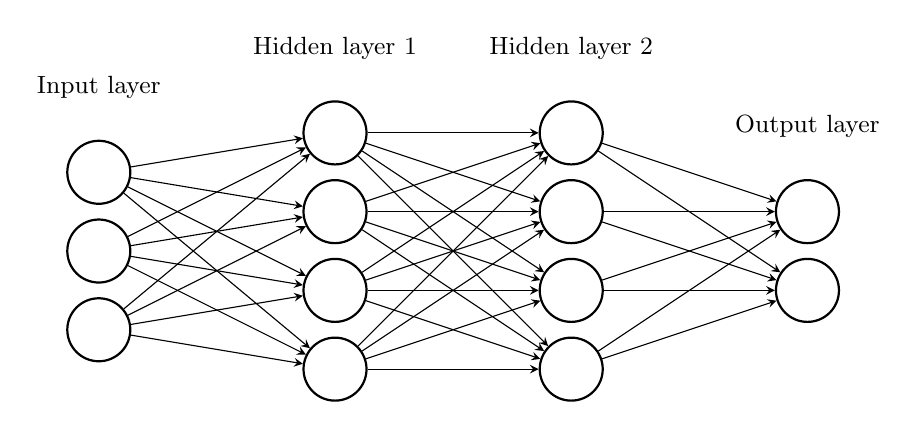
\begin{tikzpicture}[
    neuron/.style={circle, draw, thick, minimum size=8mm},
    layerlabel/.style={font=\small},
    >=stealth
]

% ----- Input layer -----
\foreach \i in {1,...,3}{
    \node[neuron] (I\i) at (0,2-\i) {};
}
\node[layerlabel, above=4mm of I1] {Input layer};

% ----- Hidden layer 1 -----
\foreach \i in {1,...,4}{
    \node[neuron] (H1\i) at (3,2.5-\i) {};
}
\node[layerlabel, above=4mm of H11] {Hidden layer 1};

% ----- Hidden layer 2 -----
\foreach \i in {1,...,4}{
    \node[neuron] (H2\i) at (6,2.5-\i) {};
}
\node[layerlabel, above=4mm of H21] {Hidden layer 2};

% ----- Output layer -----
\foreach \i in {1,...,2}{
    \node[neuron] (O\i) at (9,1.5-\i) {};
}
\node[layerlabel, above=4mm of O1] {Output layer};

% ----- Connections -----
\foreach \i in {1,...,3}{
    \foreach \j in {1,...,4}{
        \draw[->, thin] (I\i) -- (H1\j);
    }
}

\foreach \i in {1,...,4}{
    \foreach \j in {1,...,4}{
        \draw[->, thin] (H1\i) -- (H2\j);
    }
}

\foreach \i in {1,...,4}{
    \foreach \j in {1,...,2}{
        \draw[->, thin] (H2\i) -- (O\j);
    }
}

\end{tikzpicture}

\caption{An example of a feedforward neural network for the following architecture:
$L = 4$, $N_0 = 3$, $N_1 = N_2 = 4$, and $N_3 = 2$.}
\label{fig:ffnn_tikz}
\end{figure}

\begin{definition}[Class of neural networks with fixed activation]
\label{def:NN_class}
Fix an activation function $\sigma$ and an architecture $(L,N_0,\dots,N_L)$ as in Definition~\ref{def:ffnn}. 
For each $M\in\mathbb N$ let $\Theta_M\subset\mathbb R^{q(M)}$ be a parameter set, where $q(M)\in\mathbb N$ denotes the number of free weights and biases. 
We denote by
\[
    \mathcal{NN}^{\sigma}_{M,N_0,N_L}
    :=
    \bigl\{ F^\theta : \mathbb R^{N_0}\to\mathbb R^{N_L} \,\big|\, \theta\in\Theta_M \bigr\}
\]
the corresponding \emph{class of neural networks} from Definition~\ref{def:ffnn} with activation $\sigma$ and architecture $(L,N_0,\dots,N_L)$, parametrised by $\theta\in\Theta_M$. 
The sequence $\{\mathcal{NN}^\sigma_{M,N_0,N_L}\}_{M\in\mathbb N}$ is interpreted as an increasing family of models of growing complexity.
\end{definition}

\subsubsection{Activation Functions}

Neural networks rely on nonlinear transformations to approximate complex functions \cite{HighamHigham2019DeepLearning}. 
Without nonlinearity, a feedforward network composed only of affine mappings would reduce to a single affine transformation and therefore lack expressive power \cite{Hornik1991}. 
Activation functions introduce this essential nonlinearity, enabling neural networks to approximate highly irregular functions, capture nonlinear dependencies in data, and satisfy the conditions required for universal approximation \cite{Hornik1991,HighamHigham2019DeepLearning}. 
Important properties include measurability, non‐constancy, and, in certain formulations of universal approximation theorems, boundedness or continuity \cite{Hornik1991, HighamHigham2019DeepLearning}.


\begin{definition}[Activation function]
\label{def:activation_function}
An \emph{activation function} is a measurable function $\sigma:\mathbb{R}\to\mathbb{R}$ applied componentwise to vectors. 
Given an affine transformation $W(x)=Ax+b$, a neuron produces the output $\sigma(W(x))$, and a layer of neurons applies $\sigma$ to each coordinate of $W(x)$ independently.
\end{definition}

\paragraph{Examples.}

\begin{figure}[h!]
\centering

% ReLU
\begin{tikzpicture}[scale=0.8]
  \draw[->] (-3,0) -- (3.2,0) node[right] {$x$};
  \draw[->] (0,-0.5) -- (0,3) node[above] {ReLU$(x)$};
  \draw[thick] (-3,0) -- (0,0);
  \draw[thick] (0,0) -- (3,3);
\end{tikzpicture}
\hspace{1.5cm}
% tanh
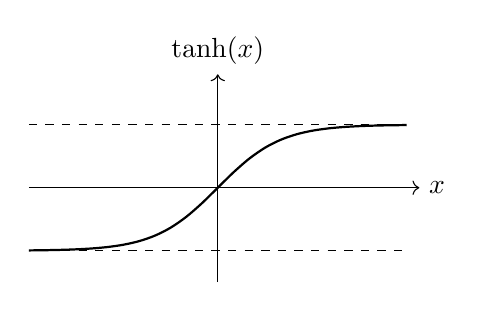
\begin{tikzpicture}[scale=0.8]
  \draw[->] (-3,0) -- (3.2,0) node[right] {$x$};
  \draw[->] (0,-1.5) -- (0,1.8) node[above] {$\tanh(x)$};
  \draw[dashed] (-3,1) -- (3,1);
  \draw[dashed] (-3,-1) -- (3,-1);
  \draw[thick, domain=-3:3, smooth] plot (\x,{tanh(\x)});
\end{tikzpicture}

\vspace{8mm}

% sigmoid
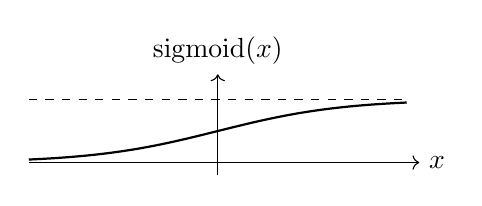
\begin{tikzpicture}[scale=0.8]
  \draw[->] (-3,0) -- (3.2,0) node[right] {$x$};
  \draw[->] (0,-0.2) -- (0,1.4) node[above] {$\mathrm{sigmoid}(x)$};
  \draw[dashed] (-3,1) -- (3,1);
  \draw[thick, domain=-3:3, smooth] plot (\x,{1/(1+exp(-\x))});
\end{tikzpicture}

\caption{Common activation functions: ReLU, $\tanh$, and the logistic sigmoid.}
\label{fig:activations}
\end{figure}

The ReLU function $\sigma(x)=\max\{0,x\}$ is popular in deep learning because it is simple, fast to compute, and helps reduce vanishing-gradient problems.
The hyperbolic tangent $\tanh(x)$ and the logistic sigmoid function $\sigma(x)=1/(1+e^{-x})$ are smooth alternatives that map real numbers to bounded intervals. These functions were more common in earlier neural network designs.

\paragraph{Universal approximation conditions.}
The Universal Approximation Theorem usually needs the activation function to be non-constant \cite{Hornik1991}. Depending on the version, it may also need to be continuous and either bounded or meet some mild regularity conditions \cite{Hornik1991,HighamHigham2019DeepLearning}.
With these assumptions, the set of functions created by feedforward neural networks is dense in certain function spaces, like $L^p$ spaces or the space of continuous functions on compact sets \cite{Hornik1991}.
This means neural networks can closely approximate many measurable functions \cite{Hornik1991,HighamHigham2019DeepLearning}. This ability makes them useful as flexible parametric models for trading strategies \cite{Buehler2019DeepHedging}.

\begin{remark}[Modern activation functions]\label{rem:modern_activations}
Modern deep-learning architectures often use ReLU variants like leaky ReLU, ELU, or GELU. These functions help improve gradient flow and make training in deep networks more stable.
These functions were first introduced to improve performance in practice. However, they also meet the basic measurability and nonlinearity requirements needed for universal approximation, so they fit well into the theoretical framework of this dissertation.
\end{remark}

\subsubsection{Universal Approximation Theorem}
Neural networks are powerful in mathematics because they can create many types of nonlinear functions that approximate a wide variety of relationships.
The Universal Approximation Theorem explains this power by showing that sufficiently large feedforward neural networks can closely approximate measurable or continuous functions.
This result provides the theoretical foundation for employing neural networks as flexible parametric representations of trading strategies \cite{Buehler2019DeepHedging,Horvath2021DeepRough,HighamHigham2019DeepLearning}.

\begin{theorem}[Universal approximation \cite{Hornik1991}]
\label{thm:universal_approx_new}
Suppose that the activation function $\sigma:\mathbb{R}\to\mathbb{R}$ is bounded and non-constant.  
Then the following properties hold:

\begin{enumerate}
    \item For any finite measure $\mu$ on $(\mathbb{R}^{d_0},\mathcal{B}(\mathbb{R}^{d_0}))$ and any $1 \le p < \infty$, the class of neural networks
    \[
        \mathcal{NN}^{\sigma}_{\infty,d_0,d_1}
    \]
    is dense in $L^p(\mathbb{R}^{d_0},\mu)$.

    \item If, in addition, $\sigma$ is continuous, then  
    \[
        \mathcal{NN}^{\sigma}_{\infty,d_0,d_1}
    \]
    is dense in $C(\mathbb{R}^{d_0})$ for the topology of uniform convergence on compact sets.
\end{enumerate}
\end{theorem}

\begin{proof}
See Appendix~\ref{app:proofs}, Proof of Theorem~\ref{thm:universal_approx_new}.
\end{proof}

\begin{remark}[Meaning of ``dense in $L^p$'' and ``uniform on compacts'']\label{rem:density}
A class of functions $\mathcal{F}$ is \emph{dense in $L^p(\mu)$} if for every $f\in L^p(\mu)$ and every $\varepsilon>0$ there exists $g\in\mathcal{F}$ such that $\|f-g\|_{L^p(\mu)}<\varepsilon$. 
Similarly, density in $C(K)$ with uniform convergence on compact sets means that for every continuous $f$ on a compact set $K$ and every $\varepsilon>0$, there is a neural network $g$ with $\sup_{x\in K}|f(x)-g(x)|<\varepsilon$. 
These notions ensure that neural networks can approximate target functions as closely as desired.
\end{remark}

\begin{remark}[Nested families of neural networks]
\label{rem:nested_families_NN}
For computational purposes it is convenient to restrict the class 
$\mathcal{NN}^{\sigma}_{\infty,d_0,d_1}$  
to an increasing sequence of finite-dimensional subclasses
\[
    \{\mathcal{NN}^{\sigma}_{M,d_0,d_1}\}_{M\in\mathbb{N}},
\]
where each network class is parametrised by a vector 
$\theta \in \Theta_{M,d_0,d_1} \subset \mathbb{R}^{k(M)}$ for some $k(M)\in\mathbb{N}$.  
These subclasses satisfy:

\begin{enumerate}
    \item $\mathcal{NN}^{\sigma}_{M,d_0,d_1} \subset \mathcal{NN}^{\sigma}_{M+1,d_0,d_1}$ for all $M\in\mathbb{N}$,
    \item $\displaystyle \bigcup_{M\in\mathbb{N}} \mathcal{NN}^{\sigma}_{M,d_0,d_1} 
    = \mathcal{NN}^{\sigma}_{\infty,d_0,d_1}$,
    \item for every $M\in\mathbb{N}$,
    \[
        \mathcal{NN}^{\sigma}_{M,d_0,d_1}
        =
        \{ F^\theta : \theta \in \Theta_{M,d_0,d_1} \}.
    \]
\end{enumerate}

These properties ensure that increasing the network size enlarges the representational capacity while preserving the density guaranteed by Theorem~\ref{thm:universal_approx_new}.
\end{remark}

\paragraph{Deep vs.\ wide networks.}
The Universal Approximation Theorem applies to networks with a single hidden layer, but such networks may require an extremely large number of neurons to achieve good approximation accuracy \cite{Hornik1991}. 
Networks with more hidden layers can often represent complex functions using far fewer parameters and can generalize better \cite{HighamHigham2019DeepLearning}. 
This balance between depth and width is key in modern deep learning. Depth provides the network with structure, while width increases its ability to express diverse functions \cite{HighamHigham2019DeepLearning}.

\begin{remark}[Practical relevance in mathematical finance]\label{rem:practical_nn_finance}
From a hedging perspective, the theorem demonstrates that neural networks can approximate optimal trading strategies, which are often complex, nonlinear, and path-dependent \cite{Buehler2019DeepHedging,Horvath2021DeepRough,HighamHigham2019DeepLearning}. 
This result provides justification for employing neural networks in frameworks such as deep hedging, where trading strategies are represented as parametric functions that learn nonlinear relationships between market data and portfolio adjustments \cite{Buehler2019DeepHedging}. 
The theorem therefore supports the conclusion that, with adequate training and model capacity, neural networks can approximate near-optimal hedging rules under a range of risk criteria \cite{Buehler2019DeepHedging,HighamHigham2019DeepLearning}.
\end{remark}

\subsubsection{Stochastic Gradient Descent and Backpropagation}

Once a parametric class of neural-network trading strategies and an objective functional are set \cite{Buehler2019DeepHedging}. 
In our framework this objective is induced by a convex risk measure, such as an OCE/AVaR-type criterion, because convexity yields a coherent notion of preference, preserves diversification effects, and leads to stable optimisation problems that are well aligned with risk management practice \cite{FoellmerSchied2016,Buehler2019DeepHedging}. 
However, the numerical training procedure described below does not need the objective to be convex in the network parameters. Neural-network training is naturally non-convex, and stochastic gradient methods are used on the resulting non-convex empirical objective as usual \cite{HighamHigham2019DeepLearning,KingmaBa2015Adam}.
The hedging problem then turns into numerically minimizing an empirical loss function \cite{HighamHigham2019DeepLearning}.
This section describes the optimization tools used to train these models.
In practice, stochastic gradient methods are used to train neural networks \cite{HighamHigham2019DeepLearning,KingmaBa2015Adam}.
These methods allow efficient handling of large sets of simulations and help the model learn complex, nonlinear trading rules \cite{Buehler2019DeepHedging,Horvath2021DeepRough}.

\begin{definition}[Empirical risk]
\label{def:empirical_risk}
Given $N$ simulated paths and a loss function $\ell$, the \emph{empirical risk} of a neural-network–parametrised strategy $\theta$ is defined by
\[
\widehat{\rho}_{N}(\theta)
    :=
    \inf_{w\in\mathbb{R}}
    \left\{
        w + \frac{1}{N}\sum_{i=1}^{N}
        \ell\!\left(X^{(i)}(\theta) - w\right)
    \right\},
\]
where $X^{(i)}(\theta)$ is the terminal P\&L of the strategy on the $i$th simulated price path.
Training the network consists in finding $\theta$ that minimises $\widehat{\rho}_{N}(\theta)$.
\end{definition}

\paragraph{Mini-batch stochastic gradient descent: intuition.}
Calculating the gradient of $\widehat{\rho}_N(\theta)$ with all $N$ samples can be costly, especially if $N$ is large or the network is deep.
Mini-batch stochastic gradient descent (SGD) estimates the full gradient by using a small random set of samples. This lets the model update its parameters more often and speeds up training.
\begin{figure}[h!]
\centering
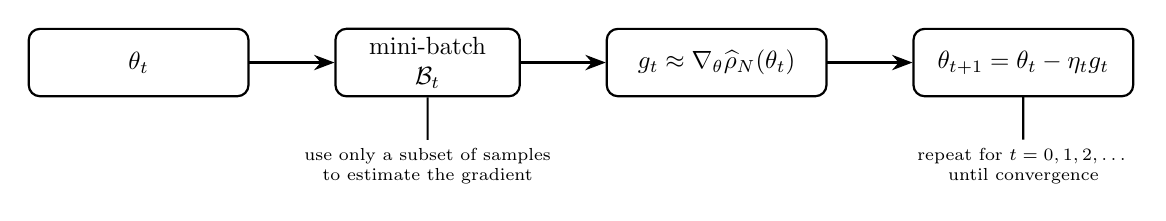
\begin{tikzpicture}[
    scale=0.9,
    every node/.style={transform shape},
    box/.style={draw, thick, rounded corners, minimum width=3.1cm, minimum height=0.95cm, align=center},
    small/.style={draw, thick, rounded corners, minimum width=2.6cm, minimum height=0.85cm, align=center},
    arr/.style={-{Stealth[length=2.6mm]}, thick},
    node distance=1.2cm
]

\node[box] (theta) {$\theta_t$};
\node[small, right=of theta] (batch) {mini-batch\\$\mathcal{B}_t$};
\node[box, right=of batch] (grad) {$g_t \approx \nabla_\theta \widehat{\rho}_N(\theta_t)$};
\node[box, right=of grad] (update) {$\theta_{t+1}=\theta_t-\eta_t g_t$};

\draw[arr] (theta) -- (batch);
\draw[arr] (batch) -- (grad);
\draw[arr] (grad) -- (update);

\node[below=6mm of batch, font=\scriptsize, align=center] (note1)
{use only a subset of samples\\to estimate the gradient};
\draw[-, thick] (batch.south) -- (note1.north);

\node[below=6mm of update, font=\scriptsize, align=center] (note2)
{repeat for $t=0,1,2,\dots$\\until convergence};
\draw[-, thick] (update.south) -- (note2.north);

\end{tikzpicture}
\caption{One iteration of mini-batch stochastic gradient descent. The gradient is estimated on a randomly sampled mini-batch and used to update the parameter vector.}
\label{fig:sgd_step}
\end{figure}


\paragraph{Mini-batch SGD: formal description.}
Let $\mathcal{B}_t\subset\{1,\dots,N\}$ be a randomly selected mini-batch at iteration $t$. 
The stochastic gradient descent update takes the form
\[
\theta_{t+1}
    =
    \theta_t 
    - \eta_t\,
    \nabla_{\theta}
    \left[
        \frac{1}{|\mathcal{B}_t|}
        \sum_{i\in\mathcal{B}_t}
        \ell\!\left(X^{(i)}(\theta_t)\right)
    \right],
\]
where $\eta_t>0$ is the learning rate. 
The mini-batch gradient is an unbiased estimator of the full gradient, and its variance helps the optimisation escape shallow local minima or flat regions.
\begin{figure}[h!]
\centering
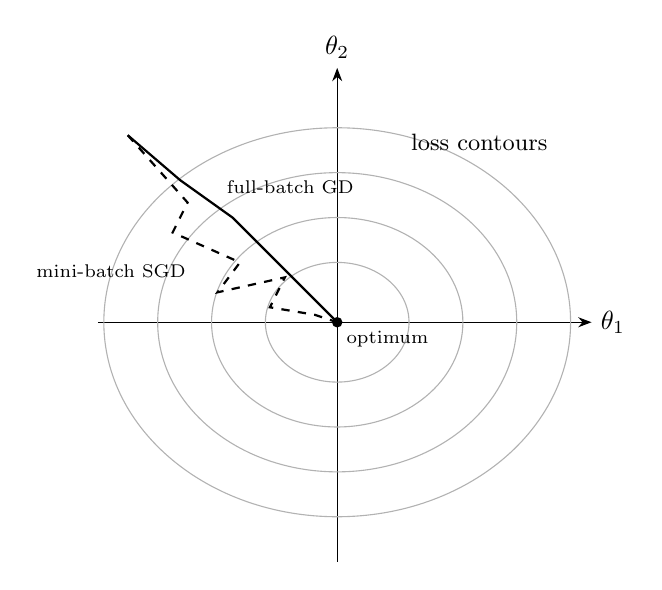
\begin{tikzpicture}[
    scale=0.95,
    every node/.style={transform shape},
    >=Stealth
]

\draw[->] (-3.2,0) -- (3.4,0) node[right] {$\theta_1$};
\draw[->] (0,-3.2) -- (0,3.4) node[above] {$\theta_2$};

\foreach \r in {0.8,1.4,2.0,2.6}{
    \draw[gray!60] (0,0) ellipse ({1.2*\r} and {\r});
}

\node at (1.9,2.4) {\small loss contours};

\draw[thick]
(-2.8,2.5)
-- (-2.1,1.9)
-- (-1.4,1.4)
-- (-0.9,0.9)
-- (-0.5,0.5)
-- (-0.2,0.2)
-- (0,0);

\node[above right] at (-1.6,1.6) {\scriptsize full-batch GD};

\draw[thick,dashed]
(-2.8,2.5)
-- (-2.0,1.6)
-- (-2.2,1.2)
-- (-1.3,0.8)
-- (-1.6,0.4)
-- (-0.7,0.6)
-- (-0.9,0.2)
-- (-0.3,0.1)
-- (0,0);

\node[below left] at (-1.9,0.9) {\scriptsize mini-batch SGD};

\fill (0,0) circle (2pt);
\node[below right] at (0,0) {\scriptsize optimum};

\end{tikzpicture}
\caption{Comparison of full-batch gradient descent and mini-batch stochastic gradient descent. 
Full-batch updates follow a smooth trajectory, while mini-batch updates exhibit stochastic fluctuations due to gradient noise.}
\label{fig:gd_vs_sgd}
\end{figure}
\FloatBarrier

\paragraph{Backpropagation.}
The gradient $\nabla_{\theta}\ell(X^{(i)}(\theta))$ is computed using \emph{backpropagation}, an algorithm based on repeated applications of the chain rule. 
Given the forward computation through layers
\[
h^{(\ell)}=\sigma\!\left(A^{(\ell)}h^{(\ell-1)} + b^{(\ell)}\right),
\]
the algorithm propagates derivatives backward from the output to earlier layers:
\[
\frac{\partial \ell}{\partial A^{(\ell)}}
    =
    \left(\frac{\partial \ell}{\partial h^{(\ell)}} 
    \odot \sigma'\!\left(A^{(\ell)}h^{(\ell-1)} + b^{(\ell)}\right)\right)
    \left(h^{(\ell-1)}\right)^{\!\top},
\]
and similarly for $\partial \ell/\partial b^{(\ell)}$. 
This yields all parameter gradients needed for SGD updates.
\begin{figure}[h!]
\centering
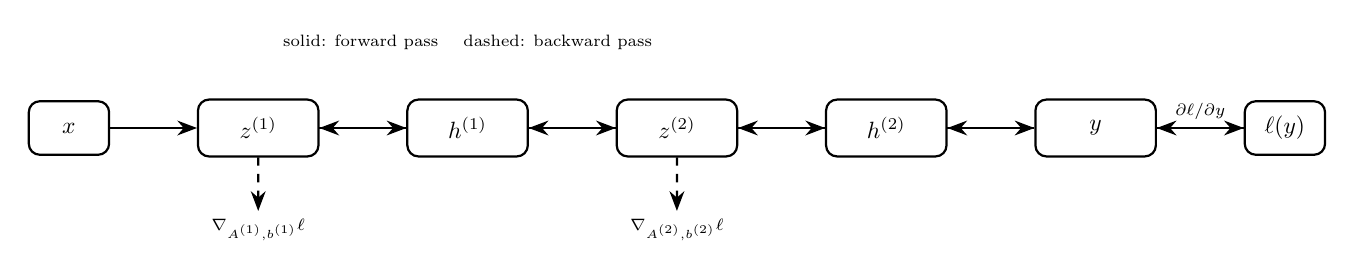
\begin{tikzpicture}[
    scale=0.85,
    every node/.style={transform shape},
    box/.style={draw, thick, rounded corners, minimum width=1.8cm, minimum height=0.85cm, align=center},
    smallbox/.style={draw, thick, rounded corners, minimum width=1.2cm, minimum height=0.8cm, align=center},
    fwd/.style={-{Stealth[length=2.5mm]}, thick},
    bwd/.style={-{Stealth[length=2.5mm]}, thick, dashed},
    node distance=1.3cm
]

\node[smallbox] (x) {$x$};
\node[box, right=of x] (z1) {$z^{(1)}$};
\node[box, right=of z1] (h1) {$h^{(1)}$};
\node[box, right=of h1] (z2) {$z^{(2)}$};
\node[box, right=of z2] (h2) {$h^{(2)}$};
\node[box, right=of h2] (y) {$y$};
\node[smallbox, right=of y] (loss) {$\ell(y)$};

\draw[fwd] (x) -- (z1);
\draw[fwd] (z1) -- (h1);
\draw[fwd] (h1) -- (z2);
\draw[fwd] (z2) -- (h2);
\draw[fwd] (h2) -- (y);
\draw[fwd] (y) -- (loss);

\draw[bwd] (loss) -- node[above, font=\scriptsize] {$\partial\ell/\partial y$} (y);
\draw[bwd] (y) -- (h2);
\draw[bwd] (h2) -- (z2);
\draw[bwd] (z2) -- (h1);
\draw[bwd] (h1) -- (z1);

\node[below=0.8cm of z1, font=\scriptsize] (grad1) {$\nabla_{A^{(1)},b^{(1)}}\ell$};
\node[below=0.8cm of z2, font=\scriptsize] (grad2) {$\nabla_{A^{(2)},b^{(2)}}\ell$};

\draw[bwd] (z1.south) -- (grad1.north);
\draw[bwd] (z2.south) -- (grad2.north);

\node[above=6mm of h1, font=\scriptsize] {solid: forward pass \quad dashed: backward pass};

\end{tikzpicture}

\caption{Forward and backward passes in a feedforward neural network. The forward pass computes layer outputs, while the backward pass propagates derivatives by the chain rule to obtain gradients with respect to network parameters.}
\label{fig:backprop_flow}
\end{figure}
\FloatBarrier

\paragraph{Adam: an adaptive optimisation method.}
Although SGD is simple, its performance is sensitive to the learning rate.  
Adam (\cite{KingmaBa2015Adam}) addresses this by maintaining exponential moving averages of the gradient and its squared value:
\[
m_{t} = \beta_1 m_{t-1} + (1-\beta_1)\, g_t,
\qquad
v_{t} = \beta_2 v_{t-1} + (1-\beta_2)\, g_t^{2},
\]
where $g_t$ is the mini-batch gradient. 
The update takes the form
\[
\theta_{t+1}
=
\theta_t 
- \eta \frac{m_t/(1-\beta_1^{t})}{\sqrt{v_t/(1-\beta_2^{t})}+\varepsilon}.
\]
Adam adapts the step size for each parameter individually and typically converges more robustly than vanilla SGD.
\begin{figure}[h!]
\centering
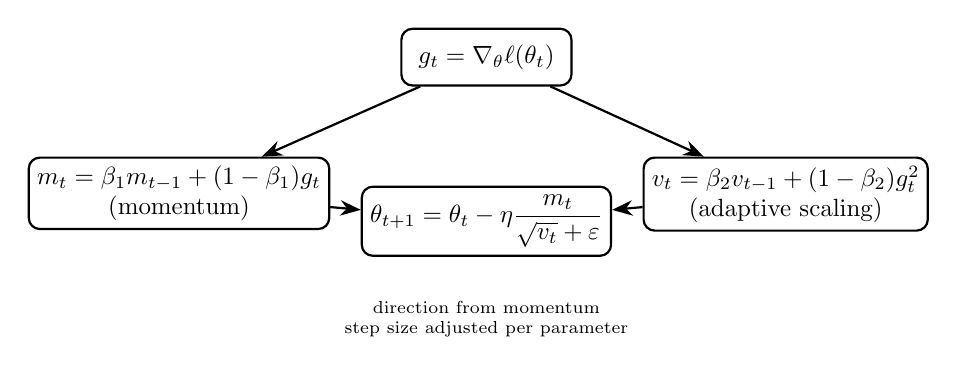
\begin{tikzpicture}[
    scale=0.9,
    every node/.style={transform shape},
    box/.style={draw, thick, rounded corners, minimum width=3.2cm, minimum height=0.9cm, align=center},
    small/.style={draw, thick, rounded corners, minimum width=2.4cm, minimum height=0.8cm, align=center},
    arr/.style={-{Stealth[length=2.6mm]}, thick},
    node distance=1.4cm
]

\node[small] (grad) {$g_t = \nabla_\theta \ell(\theta_t)$};

\node[box, below left=of grad] (m)
{$m_t = \beta_1 m_{t-1} + (1-\beta_1) g_t$\\(momentum)};

\node[box, below right=of grad] (v)
{$v_t = \beta_2 v_{t-1} + (1-\beta_2) g_t^2$\\(adaptive scaling)};

\node[box, below=1.4cm of grad] (update)
{$\displaystyle
\theta_{t+1}
=
\theta_t
-
\eta
\frac{m_t}{\sqrt{v_t}+\varepsilon}
$};

\draw[arr] (grad) -- (m);
\draw[arr] (grad) -- (v);
\draw[arr] (m) -- (update);
\draw[arr] (v) -- (update);

\node[below=5mm of update, font=\scriptsize, align=center]
{direction from momentum \\ step size adjusted per parameter};

\end{tikzpicture}
\caption{Illustration of the Adam optimiser combining momentum and adaptive learning rates. 
The first moment estimate smooths the gradient direction, while the second moment rescales updates to stabilise training.}
\label{fig:adam_optimizer}
\end{figure}
\FloatBarrier

\begin{remark}[Automatic differentiation in PyTorch]\label{rem:auto_diff}
In real-world applications, people rarely implement the backpropagation algorithm manually.
Modern machine learning frameworks such as PyTorch and TensorFlow automatically compute gradients using reverse-mode \emph{automatic differentiation}. This method efficiently computes $\nabla_{\theta}\widehat{\rho}_N(\theta)$ regardless of the network's depth.
As a result, using gradients to train hedging strategies is both practical and scalable.
\end{remark}

\subsubsection{Neural Networks as Parametrised Hedging Strategies}
The universal approximation property of neural networks supports their use as flexible models to represent trading strategies \cite{Hornik1991,HighamHigham2019DeepLearning}. 
In discrete-time hedging, strategies depend on available information. Neural networks provide a practical way to approximate these strategies without strict assumptions about their form \cite{Buehler2019DeepHedging,Horvath2021DeepRough}. 
This section explains how to build trading strategies using neural networks and shows how these strategies create finite-dimensional versions of the possible strategy space \cite{Buehler2019DeepHedging}.

\begin{definition}[Neural-network trading strategies]
\label{def:NN_trading_strategies_new}
Let $\mathcal{H}$ denote the \emph{set of admissible trading strategies}, and let 
$I_k$ represents the information available at time $t_k$.  
For a fixed $M \in \mathbb{N}$ we define the \emph{family of neural-network trading strategies} by
\[
\mathcal{H}_M
=
\left\{
    (\delta_k)_{k=0,\dots,n-1} \in \mathcal{H}
    :
    \delta_k = F_k(I_0,\dots,I_k,\delta_{k-1}),\;
    F_k \in \mathcal{NN}^{\sigma}_{M,\,r(k+1)+d,\,d}
\right\}
\]
\[
=
\left\{
    (\delta_k)_{k=0,\dots,n-1} \in \mathcal{H}
    :
    \delta_k = F_k^{\theta_k}(I_0,\dots,I_k,\delta_{k-1}),\;
    \theta_k \in \Theta_{M,\,r(k+1)+d,\,d}
\right\},
\]
with the convention $\delta_{-1}=0$.
Thus, each position update $\delta_k$ is produced by a neural network that maps the available information and the previous portfolio position into new holdings in the $d$ traded instruments.
\end{definition}
\begin{remark}\label{rem:nn_tractability}
The optimisation problem becomes tractable once the infinite-dimensional space $\mathcal{H}$ is replaced by the finite-dimensional subset $\mathcal{H}_M$. 
With the representation
\[
\mathcal{H}_M
=
\left\{
(\delta_k)_{k=0,\dots,n-1} \in \mathcal{H}
:\,
\delta_k = F_k^{\theta_k}(I_0,\dots,I_k,\delta_{k-1}),\;
\theta_k \in \Theta_{M,r(k+1)+d,d}
\right\},
\]
the optimal hedging problem reduces to minimising the risk functional over the parameter set $\Theta_M = \prod_{k=0}^{n-1} \Theta_{M,r(k+1)+d,d}$. 
Thus, the infinite-dimensional optimisation over trading strategies is replaced by a finite-dimensional optimisation over neural-network parameters.
\end{remark}

\begin{remark}\label{rem:no_markov_required}
Note that no Markovian assumption on the price process is required. 
In particular, $S$ need not be an $(\mathcal{F},\mathbb{P})$-Markov process, and the payoff $X$ may depend on $S_T$ only through an arbitrary Borel payoff function $g:\mathbb{R}^{d}\to\mathbb{R}$.  
This allows the optimal strategy to be written as
\[
\delta_k = f_k(I_k,\delta_{k-1})
\]
for some measurable functions $f_k : \mathbb{R}^{r+d} \to \mathbb{R}^{d}$, which neural networks can approximate arbitrarily well.
\end{remark}

\begin{remark}[Interpretation of parametrised strategies]\label{rem:parametrised_strategies}
The map $\delta_k = F^{\theta_k}_k(I_0,\dots,I_k,\delta_{k-1})$ describes a trading rule that depends on the entire history of observed information as well as the previous portfolio position. 
Representing this rule by a neural network allows the hedger to learn complex, highly nonlinear mappings that may not admit closed-form expressions. 
This flexibility is essential when optimal hedging decisions depend on features such as implied volatility, rough volatility effects, transaction costs, or higher-order path characteristics.
\end{remark}

\paragraph{Density of neural-network strategies.}
The Universal Approximation Theorem implies that, as $M$ increases, the families $\mathcal{H}_M$ approximate $\mathcal{H}$ in a suitable sense. 
In particular, optimal strategies that depend measurably on observed information can be approximated arbitrarily well by neural networks.

\begin{proposition}[Consistency of neural-network hedging strategies]
\label{prop:NN_consistency}
Let $\pi(X)$ denote the minimal risk-based price defined over all admissible strategies, and let $\pi^{M}(X)$ be its neural-network approximation. 
Then
\[
    \lim_{M \to \infty} \pi^{M}(X) = \pi(X).
\]
\end{proposition}

\begin{proof}
See Appendix~\ref{app:proofs}, Proof of Proposition~\ref{prop:NN_consistency}.
\end{proof}

\begin{remark}[Practical relevance]\label{rem:nn_practical_relevance}
This framework justifies neural networks as powerful approximators of optimal hedging rules, especially when the true optimal strategy exhibits nonlinear or path-dependent behaviour. 
It bridges the gap between theoretical hedging frameworks and practical algorithms capable of operating in markets with frictions, rough volatility, and incomplete information.
\end{remark}

\subsubsection{Numerical Approximation of Optimal Hedging Strategies}

The previous subsections introduced the risk-based pricing functional, the class of admissible trading strategies, and their neural-network parametrisation. 
In this subsection we combine these ingredients and describe how the minimal risk-based price is approximated numerically.
The approach follows the deep hedging framework of \cite{Buehler2019DeepHedging} and its extension to rough-volatility markets in \cite{Horvath2021DeepRough}.

\begin{figure}[!ht]
\centering
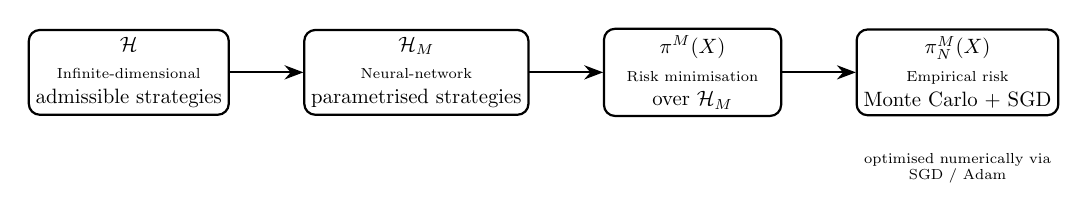
\begin{tikzpicture}[
    scale=0.75,
    every node/.style={transform shape},
    box/.style={draw, thick, rounded corners, minimum width=3.0cm, minimum height=0.95cm, align=center},
    arr/.style={-{Stealth[length=2.4mm]}, thick},
    node distance=1.25cm
]

\node[box] (H)
{$\mathcal H$\\[0.5mm]
\scriptsize Infinite-dimensional\\admissible strategies};

\node[box, right=of H] (HM)
{$\mathcal H_M$\\[0.5mm]
\scriptsize Neural-network\\parametrised strategies};

\node[box, right=of HM] (piM)
{$\pi^M(X)$\\[0.5mm]
\scriptsize Risk minimisation\\over $\mathcal H_M$};

\node[box, right=of piM] (piMN)
{$\pi^M_N(X)$\\[0.5mm]
\scriptsize Empirical risk\\Monte Carlo + SGD};

\draw[arr] (H) -- (HM);
\draw[arr] (HM) -- (piM);
\draw[arr] (piM) -- (piMN);

\node[below=5mm of piMN, font=\scriptsize, align=center]
{optimised numerically via\\SGD / Adam};

\end{tikzpicture}
\caption{From the infinite-dimensional hedging problem to its numerical approximation.}
\label{fig:nn_pipeline}
\end{figure}

\FloatBarrier

Recall from Section~\ref{subsec:convex_risk_measures} that the minimal risk-based price of a liability $X$ is given by
\begin{equation}
\pi(X)
:=
\inf_{\delta\in\mathcal H}
\rho\bigl(-X + (\delta\cdot S)_T - C_T(\delta)\bigr),
\label{eq:pi_again}
\end{equation}
where $\rho$ is a convex risk measure and $\mathcal H$ is the set of admissible strategies.
Replacing $\mathcal H$ by the neural-network class $\mathcal H_M$ from Definition~\ref{def:NN_trading_strategies_new} yields the finite-dimensional approximation
\begin{equation}
\pi^{M}(X)
:=
\inf_{\delta\in\mathcal H_M}
\rho\bigl(-X + (\delta\cdot S)_T - C_T(\delta)\bigr).
\label{eq:piM_NN_def}
\end{equation}
Proposition~\ref{prop:NN_consistency} shows that $\pi^{M}(X)\to\pi(X)$ as $M\to\infty$, so the approximation error from restricting to neural-network strategies can be made arbitrarily small.

\paragraph{Empirical approximation.}
In practice the risk functional $\rho$ cannot be evaluated analytically and is approximated by Monte Carlo simulation.
Let $(\Omega^{(i)})_{i=1,\dots,N}$ be i.i.d.\ samples of all relevant risk factors (price paths, volatility drivers, etc.), and denote by $X^{(i)}(\theta)$ the terminal P\&L on path $\Omega^{(i)}$ when trading with parameter vector $\theta\in\Theta_M$.
Using the OCE representation~\eqref{eq:OCE_def}, we define the empirical risk from Definition~\ref{def:empirical_risk} and set
\begin{equation}
\pi^{M}_N(X)
:=
\inf_{\theta\in\Theta_M}
\widehat{\rho}_N(\theta),
\label{eq:piMN_def}
\end{equation}
which approximates $\pi^{M}(X)$ by replacing expectations with sample averages.
Optimising~\eqref{eq:piMN_def} is carried out using stochastic gradient methods as described in Section 2.3.4.

\begin{proposition}[Consistency of empirical risk minimisation]
\label{prop:empirical_consistency}
Fix $M\in\mathbb N$ and assume that the loss function $\ell$ in~\eqref{eq:OCE_def} has at most polynomial growth and that
\[
\mathbb{E}\bigl[\ell\bigl(|X(\theta)|\bigr)\bigr] < \infty
\qquad\text{for all }\theta\in\Theta_M.
\]
Then, for any liability $X$,
\[
\pi^{M}_N(X) \xrightarrow[N\to\infty]{\text{a.s.}} \pi^{M}(X).
\]
\end{proposition}

\begin{proof}
See Appendix~\ref{app:proofs}, Proof of Proposition~\ref{prop:empirical_consistency}.
\end{proof}
\FloatBarrier
\begin{figure}[!ht]
\centering
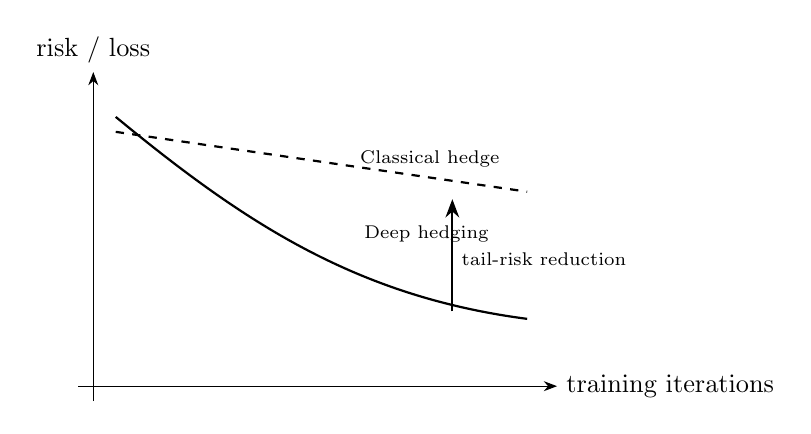
\begin{tikzpicture}[
    scale=0.95,
    every node/.style={transform shape},
    >=Stealth
]

\draw[->] (-0.2,0) -- (6.2,0) node[right] {training iterations};
\draw[->] (0,-0.2) -- (0,4.2) node[above] {risk / loss};

\draw[thick] 
(0.3,3.6) 
.. controls (2.0,2.2) and (3.5,1.2) .. 
(5.8,0.9);

\draw[thick,dashed] 
(0.3,3.4) -- (5.8,2.6);

\node[above right] at (3.5,1.8) {\scriptsize Deep hedging};
\node[above] at (4.5,2.8) {\scriptsize Classical hedge};

\draw[->, thick] (4.8,1.0) -- (4.8,2.5);
\node[right, font=\scriptsize] at (4.8,1.7) {tail-risk reduction};

\end{tikzpicture}
\caption{Conceptual illustration of numerical convergence and improved tail behaviour of neural-network hedging strategies.}
\label{fig:nn_convergence}
\end{figure}
\FloatBarrier

Combining Propositions~\ref{prop:NN_consistency} and~\ref{prop:empirical_consistency} shows that, by first choosing $M$ large enough and then increasing $N$, the numerical approximation $\pi^{M}_N(X)$ can be made arbitrarily close to the theoretical price $\pi(X)$.

\begin{remark}[Error decomposition]\label{rem:error_decomposition}
The total error between $\pi^{M}_N(X)$ and $\pi(X)$ can be viewed as the sum of three components:
\begin{itemize}
    \item the \emph{approximation error} $\pi^{M}(X)-\pi(X)$ from restricting to the class $\mathcal H_M$;
    \item the \emph{statistical error} $\pi^{M}_N(X)-\pi^{M}(X)$ from replacing expectations by empirical averages;
    \item the \emph{optimisation error} due to terminating the stochastic-gradient algorithm before reaching the global minimum of~\eqref{eq:piMN_def}.
\end{itemize}
In numerical implementations, one balances these errors by increasing $M$ and $N$ only as far as computational resources and optimisation stability permit \cite{Buehler2019DeepHedging,HighamHigham2019DeepLearning}.
\end{remark}

\begin{remark}[Practical training procedure]\label{rem:practical_training}
In applications, the numerical scheme typically proceeds as follows \cite{Buehler2019DeepHedging,Horvath2021DeepRough}:
\begin{enumerate}
    \item Simulate a large number of market scenarios under the chosen model (e.g., Black--Scholes, Heston, or rough Bergomi).
    \item Split the scenarios into \emph{training}, \emph{validation}, and \emph{test} sets.
    \item Minimise the empirical risk~\eqref{eq:piMN_def} on the training set using mini-batch stochastic gradient methods, monitoring the validation risk to avoid overfitting (for example via early stopping or regularisation).
    \item Evaluate the final strategy on the test set to obtain an unbiased estimate of the out-of-sample hedging performance.
\end{enumerate}
This workflow is directly applicable in rough-volatility models, where the main additional cost comes from simulating the non-Markovian volatility drivers \cite{Horvath2021DeepRough}.
\end{remark}

\begin{remark}[Computational advantages in rough-volatility markets]
\label{rem:computational_adv_rough}
When volatility dynamics are rough, pricing and hedging are typically more computationally demanding than in classical diffusion models. 
One main reason is non-Markovianity. In these cases, the relevant state cannot be simplified to a low-dimensional vector, which makes both model calibration and repeated calculation of hedging sensitivities more difficult \cite{GatheralRough,BayerFriz2016,Horvath2021DeepRough}.
Also, non-Markovian rough-volatility models rarely have explicit pricing formulas like those in the Black-Scholes model. As a result, option values and Greeks often have to be calculated numerically, for example using Monte Carlo methods. This can make frequent recalibration very costly \cite{BayerFriz2016,FrizGatheral2020}.
Deep hedging helps solve this computational problem by moving most of the work to one offline training phase. In this phase, a neural network learns an almost optimal trading rule from simulated scenarios based on the chosen objective \cite{Buehler2019DeepHedging,Horvath2021DeepRough}.
After training, the strategy can be used online with fast forward passes, which are matrix-vector operations. This approach works well for real-time hedging, even when the underlying dynamics are non-Markovian \cite{Buehler2019DeepHedging,Horvath2021DeepRough}.
\end{remark}

\paragraph{Transition to model specification.}
The framework in this chapter is designed to work with any model.
All definitions and results here apply to general discrete-time markets, even when there are frictions or incomplete information.
In the next chapter, we introduce rough volatility models. These will be the main test cases for evaluating how well the hedging strategies from this dissertation perform and how robust they are.

\newpage
\section{Stochastic Volatility: Rough Volatility Models}
\label{sec:rough_volatility}
This section introduces stochastic volatility models with rough paths. These models serve as the data-generating processes for the numerical experiments in this dissertation.
Rough volatility models are based on classical diffusion frameworks but allow volatility to exhibit non-Markovian, highly irregular behavior, which matches what is observed in real data.

Classical models such as the Black--Scholes \cite{BlackScholes1973} and Heston \cite{Heston1993} treat volatility as a smooth diffusion process. This makes pricing and hedging easier to study, but it does not capture important features of high-frequency volatility dynamics.
Empirical studies show that volatility is persistently rough and irregular in the short term. This has led to new models that go beyond the diffusion approach \cite{GatheralRough}.

Rough volatility models address these problems by modeling volatility as a fractional or Volterra-type process with low regularity. They are still practical for pricing and simulation \cite{BayerFriz2016,FrizGatheral2020}.
These models are now a main focus in modern quantitative finance. They provide a challenging but realistic way to test hedging strategies, especially when models are not specified correctly.

The rest of this section explains why rough volatility matters, introduces the main model types used in practice, and describes how they are simulated. This prepares for the hedging experiments in later chapters.

\subsection{Stylised Facts of Volatility}
\label{subsec:stylised_facts_volatility}

This subsection summarises empirical regularities of volatility that motivate the rough-volatility viewpoint.
The presentation follows the empirical analysis in \cite{GatheralRough}, which documents that volatility (more precisely, log-volatility) exhibits very low short-term regularity and a stable scaling behaviour across assets and sampling frequencies.

\begin{definition}[Realised variance proxy for spot variance]
\label{def:realised_variance_proxy}
Let $(P_t)_{t\ge 0}$ denote an observed asset price process and set $X_t:=\log P_t$.
Fix a window length $\Delta>0$ and an intra-window grid $t=t_0<t_1<\dots<t_m=t+\Delta$.
The \emph{realised variance} over $[t,t+\Delta]$ is
\[
\mathrm{RV}_{t,\Delta}
:=
\sum_{j=0}^{m-1}\bigl(X_{t_{j+1}}-X_{t_j}\bigr)^2.
\]
In the empirical rough-volatility literature, $\mathrm{RV}_{t,\Delta}$ (or its square root) is used as a high-frequency proxy for the latent spot variance (or volatility) at scale $\Delta$ \cite{GatheralRough}.
\end{definition}

\begin{definition}[Log-volatility and log-volatility increments]
\label{def:log_vol_increments}
Define the \emph{log-volatility proxy} by
\[
Y_{t,\Delta}:=\log\!\bigl(\mathrm{RV}_{t,\Delta}\bigr),
\]
and for a lag $h>0$ define the \emph{log-volatility increment} by
\[
\Delta_h Y_{t,\Delta}
:=
Y_{t+h,\Delta}-Y_{t,\Delta}.
\]
Empirical roughness is formulated in terms of the small-lag behaviour of these increments \cite{GatheralRough}.
\end{definition}

\begin{definition}[Second-order structure function]
\label{def:structure_function}
For $h>0$ and a fixed $\Delta>0$, define the (empirical) \emph{second-order structure function} by
\[
m_2(h)
:=
\mathbb{E}\bigl[(\Delta_h Y_{t,\Delta})^2\bigr],
\]
where the expectation is understood empirically (time-averaging under stationarity assumptions) as in \cite{GatheralRough}.
\end{definition}

\begin{remark}[Empirical roughness and scaling of log-volatility]
\label{rem:empirical_roughness_scaling}
Empirical analyses based on high-frequency volatility proxies suggest a stable power-law scaling for log-volatility increments.
In particular \cite{GatheralRough} report that there exist an exponent $H\in(0,1/2)$ and a constant $c>0$ such that, for small lags $h$,
\[
m_2(h)\approx c\,h^{2H},
\]
where $m_2(h)=\mathbb{E}\bigl[(\Delta_h Y_{t,\Delta})^2\bigr]$ is the second-order structure function from Definition~\ref{def:structure_function}.
Moreover, the estimated values of $H$ are found to be stable across assets and sampling choices, and are significantly below $1/2$ (with typical estimates around $0.1$) \cite{GatheralRough}.
\end{remark}

\begin{remark}[Interpretation of ``roughness'']
\label{rem:roughness_interpretation}
The scaling law in Remark 3.1 provides an operational notion of roughness: smaller values of $H$ correspond to more irregular short-term behaviour of log-volatility increments, while $H=1/2$ would correspond to the benchmark Brownian scaling at small lags \cite{GatheralRough}.
In the rough-volatility literature, the empirical finding $H<1/2$ is therefore interpreted as evidence that volatility is ``rough'' at short time scales \cite{GatheralRough}.
\end{remark}

\begin{proposition}[Log--log slope estimation of the roughness exponent]
\label{prop:loglog_estimation}
Assume the scaling relation in Remark 3.1 holds approximately on a range of small lags $h\in[h_{\min},h_{\max}]$.
Then
\[
\log m_2(h)\;\approx\;\log c + 2H\log h,
\]
so that $H$ can be estimated as one half of the slope of a linear regression of $\log m_2(h)$ against $\log h$ on that range, as implemented in \cite{GatheralRough}.
\end{proposition}

\begin{proof}
See Appendix~\ref{app:proofs}, Proof of Proposition~\ref{prop:loglog_estimation}.
\end{proof}

\begin{remark}[What is measured: increments of log-volatility]
\label{rem:why_log_vol}
Empirical roughness is documented for increments of \emph{log}-volatility proxies, rather than for volatility levels themselves, because the log transform stabilises scale and makes increment-based scaling diagnostics more robust across sampling choices \cite{GatheralRough}.
Accordingly, subsequent rough-volatility models are designed to reproduce the small-lag scaling of log-volatility increments described above \cite{GatheralRough}.
\end{remark}

\subsection{Failure of Classical Volatility Models}
\label{subsec:failure_classical_models}

The empirical scaling in Section~\ref{subsec:stylised_facts_volatility} suggests that log-volatility behaves much more irregularly at short time scales than a Brownian-driven diffusion \cite{GatheralRough}. 
This subsection explains why two benchmark models, Black--Scholes and Heston, do not reproduce this roughness and therefore exhibit systematic short-term misfit \cite{GatheralRough,BayerFriz2016}.

\begin{definition}[Black--Scholes model]
\label{def:black_scholes_model}
In the \emph{Black--Scholes model} the (discounted) asset price $(S_t)_{t\in[0,T]}$ satisfies
\[
dS_t = S_t\,\sigma\, dW_t,
\]
where $\sigma>0$ is a constant volatility parameter and $W$ is a Brownian motion \cite{BlackScholes1973}.
\end{definition}

\begin{definition}[Heston stochastic volatility model]
\label{def:heston_model}
In the \emph{Heston model} the pair $(S_t,V_t)_{t\in[0,T]}$ solves
\[
\frac{dS_t}{S_t} = \sqrt{V_t}\, dW_t^{(1)},
\qquad
dV_t = \kappa(\theta - V_t)\,dt + \xi \sqrt{V_t}\, dW_t^{(2)},
\]
with parameters $\kappa,\theta,\xi>0$ and correlated Brownian motions $(W^{(1)},W^{(2)})$ \cite{Heston1993}.
\end{definition}

\begin{remark}[What ``classical'' means here]
\label{rem:classical_means_brownian}
Both models are driven by Brownian noise and are Markovian in a low-dimensional state \cite{BlackScholes1973,Heston1993}. 
As discussed in \cite{GatheralRough}, this Brownian diffusion structure implies a short-term regularity consistent with a Hurst-type exponent $H=1/2$ for volatility-type signals, which conflicts with the empirical estimates $H<1/2$.
\end{remark}

\begin{proposition}[Black--Scholes cannot generate rough log-volatility]
\label{prop:bs_no_roughness}
Assume the Black--Scholes model with constant volatility $\sigma>0$ \cite{BlackScholes1973}. 
At the model level, the variance is deterministic: for any window $[t,t+\Delta]$ the integrated variance equals $\sigma^2\Delta$, hence the idealised log-variance signal is constant and its increments vanish, so
\[
m_2(h)=\mathbb{E}\bigl[(Y_{t+h,\Delta}-Y_{t,\Delta})^2\bigr]=0
\qquad\text{for all }h>0,
\]
when $Y_{t,\Delta}:=\log(\sigma^2\Delta)$.
Consequently, Black--Scholes cannot reproduce the empirical rough-volatility scaling $m_2(h)\approx c h^{2H}$ with $H\in(0,1/2)$ reported in \cite{GatheralRough}.
\end{proposition}

\begin{proof}
See Appendix~\ref{app:proofs}, Proof of Proposition~\ref{prop:bs_no_roughness}.
\end{proof}

\begin{remark}[Proxy effects]
\label{rem:bs_proxy_effect}
If $Y_{t,\Delta}$ is defined empirically via a realised-variance proxy, then $m_2(h)$ need not be zero because the proxy contains sampling noise and window-overlap effects \cite{GatheralRough}. 
These effects can produce an apparent Brownian-type scaling $m_2(h)\propto h$ even when the true volatility is constant.
This is a property of the estimator, not a volatility roughness mechanism \cite{GatheralRough}.
\end{remark}

\begin{proposition}[Diffusive scaling in Heston]
\label{prop:heston_diffusive_scaling}
In the Heston model, the variance process $V$ is a Brownian-driven diffusion \cite{Heston1993}. 
Consequently, log-volatility proxies derived from $V$ exhibit Brownian short-lag scaling, in the sense that
\[
m_2(h)\approx C h
\qquad\text{for small }h,
\]
for some constant $C>0$, which corresponds to an effective exponent $H=1/2$ and is therefore incompatible with the empirical finding $H<1/2$ in \cite{GatheralRough}.
\end{proposition}

\begin{proof}
See Appendix~\ref{app:proofs}, Proof of Proposition~\ref{prop:heston_diffusive_scaling}.
\end{proof}

\begin{remark}[Empirical misfit]
\label{rem:empirical_misfit_classical}
The scaling estimates reported in \cite{GatheralRough} are stable across assets and indicate a roughness exponent well below $1/2$. 
Propositions~\ref{prop:bs_no_roughness} and \ref{prop:heston_diffusive_scaling} show that Black--Scholes is too rigid and Heston is still too smooth at short horizons. 
This mismatch is one of the key empirical motivations for moving beyond classical diffusive volatility models \cite{GatheralRough,BayerFriz2016}.
\end{remark}

\begin{remark}[Why this matters for pricing and hedging]
\label{rem:why_misfit_matters}
Short-term irregularity of volatility impacts short-maturity option prices and hedging performance \cite{GatheralRough}. 
In particular, rough-volatility models were developed to reproduce the observed fine-scale behaviour and improve the fit of implied-volatility surfaces compared with classical diffusions \cite{GatheralRough,BayerFriz2016}. 
\end{remark}

\subsection{Rough Volatility Modelling and the Rough Bergomi Model}
\label{subsec:rough_bergomi_model}

The evidence in Section~\ref{subsec:stylised_facts_volatility} indicates that volatility is significantly rougher than what is implied by Brownian diffusions, with an effective short-term regularity parameter $H<\tfrac12$ \cite{GatheralRough}. 
A natural modelling response is to replace diffusive volatility drivers by \emph{fractional} (or more generally Volterra-type) Gaussian drivers with Hurst index $H<\tfrac12$ \cite{GatheralRough,BayerFriz2016}. 
This subsection introduces the Gaussian building block used in rough-volatility modelling and then presents the rough Bergomi model, which is a standard benchmark in this literature \cite{BayerFriz2016,RoughSurvey}.

\begin{definition}[Volterra fractional Brownian driver]
\label{def:volterra_driver}
Fix $H\in(0,\tfrac12)$ and let $W=(W_t)_{t\in[0,T]}$ be a Brownian motion. 
Define the \emph{Volterra Gaussian process}
\[
    \widetilde W^H_t
    :=
    \int_0^t (t-s)^{H-\frac12}\, dW_s,
    \qquad t\in[0,T].
\]
We also introduce the normalised version
\[
    W^H_t := \sqrt{2H}\,\widetilde W^H_t,
\]
so that $\mathbb E[(W^H_t)^2]=t^{2H}$ for all $t\in[0,T]$.
This process is often referred to as a (Riemann--Liouville) \emph{fractional Brownian motion driver} in the rough-volatility literature \cite{GatheralRough,BayerFriz2016}.
\end{definition}

\begin{proposition}[Gaussianity and covariance]
\label{prop:gaussian_covariance}
The process $(W^H_t)_{t\in[0,T]}$ from Definition~\ref{def:volterra_driver} is centred Gaussian. Moreover, for all $s,t\in[0,T]$,
\[
    \mathrm{Cov}(W^H_t,W^H_s)
    =
    2H \int_0^{s\wedge t} (t-u)^{H-\frac12}(s-u)^{H-\frac12}\, du,
\]
and in particular
\[
    \mathbb E[(W^H_t)^2]=t^{2H}.
\]
\end{proposition}

\begin{proof}
For any fixed times $0\le t_1,\dots,t_m\le T$, each random variable $W^H_{t_j}$ is an It\^o integral of a deterministic square-integrable function against Brownian motion \cite{GatheralRough,BayerFriz2016}. 
Hence any linear combination $\sum_{j=1}^m a_j W^H_{t_j}$ is again an It\^o integral and therefore Gaussian with mean zero, which implies that $(W^H_t)_{t\in[0,T]}$ is a centred Gaussian process.

For the covariance, write $t\ge s$ without loss of generality. Using the It\^o isometry,
\[
    \mathrm{Cov}(W^H_t,W^H_s)
    =
    \mathbb E[W^H_t W^H_s]
    =
    2H\,\mathbb E\!\left[
        \left(\int_0^t (t-u)^{H-\frac12}\, dW_u\right)
        \left(\int_0^s (s-u)^{H-\frac12}\, dW_u\right)
    \right]
\]
\[
    =
    2H \int_0^{s} (t-u)^{H-\frac12}(s-u)^{H-\frac12}\, du,
\]
which yields the stated formula. Setting $t=s$ gives
\[
    \mathbb E[(W^H_t)^2]
    =
    2H \int_0^{t} (t-u)^{2H-1}\, du
    =
    2H \cdot \frac{t^{2H}}{2H}
    =
    t^{2H}.
\]
\end{proof}

\begin{theorem}[H\"older regularity and short-term scaling]
\label{thm:holder_rough_driver}
Let $H\in(0,\tfrac12)$ and let $(W^H_t)_{t\in[0,T]}$ be as in Definition~\ref{def:volterra_driver}. Then:
\begin{enumerate}
    \item For every $p\ge 2$ there exists a constant $C_{p,H,T}>0$ such that for all $s,t\in[0,T]$,
    \[
        \mathbb E\bigl[|W^H_t - W^H_s|^p\bigr]
        \le
        C_{p,H,T}\,|t-s|^{pH}.
    \]
    \item For every $\alpha\in(0,H)$ there exists a modification of $W^H$ whose sample paths are $\alpha$-H\"older continuous on $[0,T]$, and no modification is $\alpha$-H\"older for any $\alpha>H$.
\end{enumerate}
These properties capture the short-term roughness mechanism used in rough-volatility models \cite{GatheralRough,BayerFriz2016}.
\end{theorem}

\begin{proof}
Let $0\le s<t\le T$ and set $\Delta:=t-s$. Using Definition~\ref{def:volterra_driver},
\[
    W^H_t - W^H_s
    =
    \sqrt{2H}\left(
        \int_0^s \bigl((t-u)^{H-\frac12}-(s-u)^{H-\frac12}\bigr)\, dW_u
        +
        \int_s^t (t-u)^{H-\frac12}\, dW_u
    \right).
\]
Since $W^H_t-W^H_s$ is Gaussian and centred, it suffices to control its variance and then use Gaussian moment equivalences.

\emph{Step 1: variance bound.}
By the It\^o isometry and the inequality $(a+b)^2\le 2a^2+2b^2$,
\[
    \mathbb E\bigl[(W^H_t-W^H_s)^2\bigr]
    \le
    4H \int_0^s \Bigl((t-u)^{H-\frac12}-(s-u)^{H-\frac12}\Bigr)^2\, du
    +
    4H \int_s^t (t-u)^{2H-1}\, du.
\]
The second integral is explicit:
\[
    \int_s^t (t-u)^{2H-1}\, du
    =
    \int_0^{\Delta} x^{2H-1}\, dx
    =
    \frac{\Delta^{2H}}{2H},
\]
so it contributes $2\Delta^{2H}$.

For the first integral, change variables $x:=s-u$ (so $x\in[0,s]$), and note that $(t-u)=(s-u)+\Delta=x+\Delta$. Hence
\[
    \int_0^s \Bigl((t-u)^{H-\frac12}-(s-u)^{H-\frac12}\Bigr)^2\, du
    =
    \int_0^s \Bigl((x+\Delta)^{H-\frac12}-x^{H-\frac12}\Bigr)^2\, dx.
\]
Split the domain into $x\in[0,\Delta]$ and $x\in[\Delta,s]$.

On $[0,\Delta]$, use $(x+\Delta)^{H-\frac12}\le (2\Delta)^{H-\frac12}$ and $x^{H-\frac12}\le \Delta^{H-\frac12}$ to get
\[
    \int_0^\Delta \Bigl((x+\Delta)^{H-\frac12}-x^{H-\frac12}\Bigr)^2 dx
    \le
    \int_0^\Delta \Bigl((2\Delta)^{H-\frac12}+\Delta^{H-\frac12}\Bigr)^2 dx
    \le
    C_{H}\,\Delta^{2H},
\]
for a constant $C_H>0$.

On $[\Delta,s]$, apply the mean value theorem to the function $f(x)=x^{H-\frac12}$: for each $x\ge \Delta$ there exists $\xi\in[x,x+\Delta]$ such that
\[
    (x+\Delta)^{H-\frac12}-x^{H-\frac12}
    =
    f'(\xi)\,\Delta
    =
    \Bigl(H-\tfrac12\Bigr)\xi^{H-\frac32}\Delta,
\]
and since $\xi\ge x\ge \Delta$ and $H-\tfrac32<0$,
\[
    \bigl|(x+\Delta)^{H-\frac12}-x^{H-\frac12}\bigr|
    \le
    \Bigl(\tfrac12-H\Bigr)\Delta\,x^{H-\frac32}.
\]
Therefore
\[
    \int_\Delta^s \Bigl((x+\Delta)^{H-\frac12}-x^{H-\frac12}\Bigr)^2 dx
    \le
    \Bigl(\tfrac12-H\Bigr)^2\Delta^2 \int_\Delta^s x^{2H-3}\, dx.
\]
Since $2H-3<-2$, the integral is finite and dominated by its lower limit:
\[
    \int_\Delta^s x^{2H-3}\, dx
    \le
    \int_\Delta^\infty x^{2H-3}\, dx
    =
    \frac{\Delta^{2H-2}}{2-2H}.
\]
Hence
\[
    \int_\Delta^s \Bigl((x+\Delta)^{H-\frac12}-x^{H-\frac12}\Bigr)^2 dx
    \le
    C_H'\,\Delta^{2H}.
\]
Combining the two pieces yields
\[
    \int_0^s \Bigl((x+\Delta)^{H-\frac12}-x^{H-\frac12}\Bigr)^2 dx
    \le
    C_H''\,\Delta^{2H}.
\]
Putting everything together, we obtain
\[
    \mathbb E\bigl[(W^H_t-W^H_s)^2\bigr]
    \le
    C_{H,T}\,|t-s|^{2H}
\]
for some constant $C_{H,T}>0$.

\emph{Step 2: $p$-moments.}
Since $W^H_t-W^H_s$ is centred Gaussian with variance bounded by $C_{H,T}\Delta^{2H}$, the Gaussian moment formula implies that for every $p\ge 2$ there exists $c_p>0$ such that
\[
    \mathbb E\bigl[|W^H_t-W^H_s|^p\bigr]
    =
    c_p\,\Bigl(\mathbb E[(W^H_t-W^H_s)^2]\Bigr)^{p/2}
    \le
    c_p\,C_{H,T}^{p/2}\,\Delta^{pH}.
\]
This proves (1).

\emph{Step 3: H\"older continuity.}
Choose $p>1/H$. Then (1) gives
\[
    \mathbb E\bigl[|W^H_t-W^H_s|^p\bigr]
    \le
    C\,|t-s|^{1+\varepsilon}
\]
with $\varepsilon=pH-1>0$. By the Kolmogorov--Chentsov theorem, there exists a modification of $W^H$ that is $\alpha$-H\"older continuous for all $\alpha\in(0,H)$.
The sharpness (no $\alpha>H$) follows from the scaling of the second moment and standard Gaussian increment arguments used in the rough-volatility literature \cite{GatheralRough,BayerFriz2016}.
\end{proof}

\begin{remark}[Kernel singularity and the role of $H$]
\label{rem:kernel_singularity}
The kernel $(t-s)^{H-\frac12}$ in Definition~\ref{def:volterra_driver} is singular at $s=t$ when $H<\tfrac12$, which creates the short-term irregularity in Theorem~\ref{thm:holder_rough_driver} \cite{GatheralRough}. 
Smaller values of $H$ correspond to a stronger singularity and therefore rougher sample paths \cite{GatheralRough,BayerFriz2016}.
\end{remark}

\begin{figure}[H]
\centering
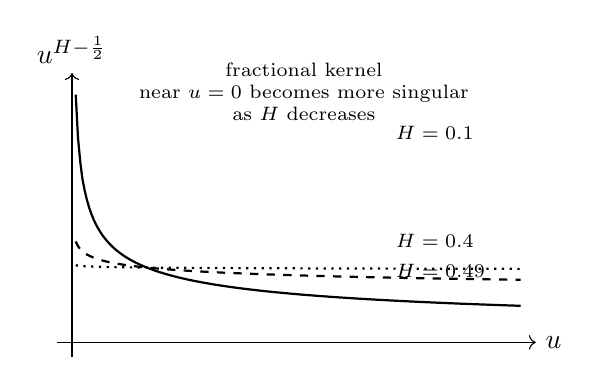
\begin{tikzpicture}[scale=0.95]
\draw[->] (-0.2,0) -- (6.2,0) node[right] {$u$};
\draw[->] (0,-0.2) -- (0,3.6) node[above] {$u^{H-\frac12}$};

\draw[thick,domain=0.05:6,samples=200] plot (\x,{pow(\x,-0.4)});
\node[font=\scriptsize, anchor=west] at (4.2,2.8) {$H=0.1$};

\draw[thick,dashed,domain=0.05:6,samples=200] plot (\x,{pow(\x,-0.1)});
\node[font=\scriptsize, anchor=west] at (4.2,1.35) {$H=0.4$};

\draw[thick,dotted,domain=0.05:6,samples=200] plot (\x,{pow(\x,-0.01)});
\node[font=\scriptsize, anchor=west] at (4.2,0.95) {$H=0.49$};

\node[font=\scriptsize, align=center] at (3.1,3.35) {fractional kernel\\near $u=0$ becomes more singular\\as $H$ decreases};

\end{tikzpicture}
\caption{Shape of the fractional kernel $u\mapsto u^{H-\frac12}$ for representative values $H<\tfrac12$. The singularity at $u=0$ is the source of short-term roughness \cite{GatheralRough,BayerFriz2016}.}
\label{fig:fractional_kernel_shapes}
\end{figure}
\FloatBarrier

\begin{definition}[Rough Bergomi variance process]
\label{def:rough_bergomi_variance}
Fix $H\in(0,\tfrac12)$ and let $(W^H_t)_{t\in[0,T]}$ be the driver from Definition~\ref{def:volterra_driver}. 
Let $\eta>0$ be a volatility-of-volatility parameter and let $\xi_0:[0,T]\to(0,\infty)$ be a deterministic forward-variance curve. 
Define the \emph{variance process} by
\begin{equation}
\label{eq:rb_variance}
    v_t
    :=
    \xi_0(t)\,
    \exp\!\left(
        \eta W^H_t - \frac12 \eta^2 t^{2H}
    \right),
    \qquad t\in[0,T].
\end{equation}
This lognormal specification is the core ingredient of the rough Bergomi model \cite{BayerFriz2016}.
\end{definition}

\begin{proposition}[Calibration property: preservation of the forward variance]
\label{prop:forward_variance_preserved}
Let $(v_t)_{t\in[0,T]}$ be defined by \eqref{eq:rb_variance}. Then for every $t\in[0,T]$,
\[
    \mathbb E[v_t] = \xi_0(t).
\]
\end{proposition}

\begin{proof}
By Proposition~\ref{prop:gaussian_covariance}, $W^H_t$ is Gaussian with mean $0$ and variance $t^{2H}$. Hence for any $\eta>0$,
\[
    \mathbb E\!\left[\exp(\eta W^H_t)\right]
    =
    \exp\!\left(\frac12 \eta^2\,\mathbb E[(W^H_t)^2]\right)
    =
    \exp\!\left(\frac12 \eta^2 t^{2H}\right).
\]
Therefore, using \eqref{eq:rb_variance},
\[
    \mathbb E[v_t]
    =
    \xi_0(t)\,
    \mathbb E\!\left[
        \exp\!\left(\eta W^H_t - \frac12 \eta^2 t^{2H}\right)
    \right]
    =
    \xi_0(t)\,
    \exp\!\left(-\frac12 \eta^2 t^{2H}\right)\,
    \exp\!\left(\frac12 \eta^2 t^{2H}\right)
    =
    \xi_0(t).
\]
\end{proof}

\begin{remark}[Why the lognormal specification is useful]
\label{rem:lognormal_useful}
The exponential form in \eqref{eq:rb_variance} ensures positivity of $v_t$ and allows the model to match a given forward-variance curve $\xi_0$ exactly via Proposition~\ref{prop:forward_variance_preserved} \cite{BayerFriz2016}. 
This separation between the roughness driver $W^H$ and the calibration input $\xi_0$ is one of the main practical advantages of the rough Bergomi construction \cite{BayerFriz2016,RoughSurvey}.
\end{remark}

\begin{definition}[Rough Bergomi price dynamics]
\label{def:rough_bergomi_price}
Let $(v_t)_{t\in[0,T]}$ be as in Definition~\ref{def:rough_bergomi_variance}. 
Let $B$ and $W$ be Brownian motions with correlation $\rho\in[-1,1]$, and define
\[
    B_t := \rho W_t + \sqrt{1-\rho^2}\,W_t^\perp,
\]
where $W^\perp$ is a Brownian motion independent of $W$. 
The \emph{rough Bergomi} model specifies the (discounted) asset \emph{price} by
\[
    dS_t = S_t \sqrt{v_t}\, dB_t,
    \qquad S_0>0,
\]
with $v_t$ driven by $W$ through \eqref{eq:rb_variance} and Definition~\ref{def:volterra_driver} \cite{BayerFriz2016}.
\end{definition}

\begin{remark}[Non-Markovianity and incompleteness]
\label{rem:non_markov_incomplete}
Because $W^H$ depends on the entire past of $W$ through a Volterra kernel, the pair $(S_t,v_t)$ is non-Markovian in finite dimension \cite{BayerFriz2016}. 
This feature is consistent with the empirical long-memory style effects highlighted in \cite{GatheralRough} and it leads to structural market incompleteness, which is one of the motivations for risk-based and learning-based hedging in incomplete markets \cite{Buehler2019DeepHedging,Horvath2021DeepRough}.
\end{remark}

\begin{figure}[H]
\centering
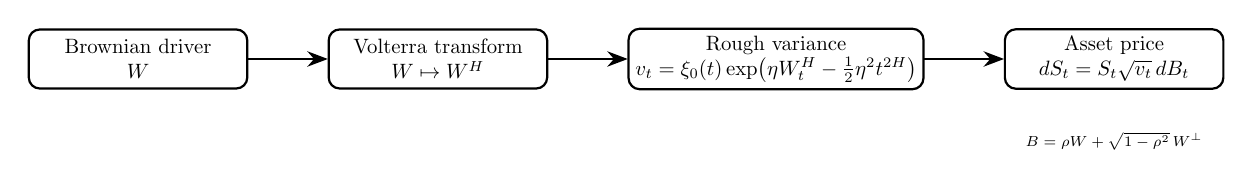
\begin{tikzpicture}[
    scale=0.75,
    every node/.style={transform shape},
    box/.style={draw, thick, rounded corners, minimum width=3.7cm, minimum height=1.0cm, align=center},
    arr/.style={-{Stealth[length=2.6mm]}, thick},
    node distance=1.35cm
]

\node[box] (W) {Brownian driver\\$W$};
\node[box, right=of W] (WH) {Volterra transform\\$W \mapsto W^H$};
\node[box, right=of WH] (v) {Rough variance\\$v_t=\xi_0(t)\exp(\eta W_t^H-\frac12\eta^2 t^{2H})$};
\node[box, right=of v] (S) {Asset price\\$dS_t=S_t\sqrt{v_t}\,dB_t$};

\draw[arr] (W) -- (WH);
\draw[arr] (WH) -- (v);
\draw[arr] (v) -- (S);

\node[below=6mm of S, font=\scriptsize, align=center]
{$B=\rho W+\sqrt{1-\rho^2}\,W^\perp$};

\end{tikzpicture}
\caption{Schematic construction of the rough Bergomi model: a Brownian motion is mapped into a rough Gaussian driver via a Volterra kernel, which generates lognormal rough variance and then drives the price \cite{BayerFriz2016,GatheralRough}.}
\label{fig:rbm_schematic}
\end{figure}
\FloatBarrier

\begin{proposition}[Conditional lognormality of variance]
\label{prop:variance_lognormal}
Fix $t\in[0,T]$. Under the rough Bergomi specification \eqref{eq:rb_variance}, the random variable $v_t$ is lognormal and
\[
    \log v_t
    =
    \log \xi_0(t) + \eta W^H_t - \frac12 \eta^2 t^{2H}.
\]
In particular, for any $q\in\mathbb R$ such that the moment exists,
\[
    \mathbb E[v_t^{\,q}]
    =
    \xi_0(t)^{q}\,
    \exp\!\left(\frac12 q(q-1)\eta^2 t^{2H}\right).
\]
\end{proposition}

\begin{proof}
The identity for $\log v_t$ is immediate from \eqref{eq:rb_variance}. Since $W^H_t$ is Gaussian by Proposition~\ref{prop:gaussian_covariance}, $\log v_t$ is Gaussian and hence $v_t$ is lognormal.

For the moment formula, use \eqref{eq:rb_variance}:
\[
    v_t^{\,q}
    =
    \xi_0(t)^q
    \exp\!\left(q\eta W^H_t - \frac12 q\eta^2 t^{2H}\right).
\]
Taking expectations and using the Gaussian exponential moment,
\[
    \mathbb E\!\left[\exp(q\eta W^H_t)\right]
    =
    \exp\!\left(\frac12 q^2 \eta^2\,\mathbb E[(W^H_t)^2]\right)
    =
    \exp\!\left(\frac12 q^2 \eta^2 t^{2H}\right),
\]
we get
\[
    \mathbb E[v_t^{\,q}]
    =
    \xi_0(t)^q
    \exp\!\left(-\frac12 q\eta^2 t^{2H}\right)
    \exp\!\left(\frac12 q^2\eta^2 t^{2H}\right)
    =
    \xi_0(t)^q \exp\!\left(\frac12 q(q-1)\eta^2 t^{2H}\right).
\]
\end{proof}

\begin{remark}[Connection to short-maturity smiles]
\label{rem:smile_connection}
Rough Bergomi was introduced to reproduce the empirically observed steep short-maturity implied-volatility skews that classical diffusions struggle to match \cite{GatheralRough,BayerFriz2016}. 
The mechanism is driven by the roughness of $W^H$ from Theorem~\ref{thm:holder_rough_driver}, which changes the scaling of volatility fluctuations at short horizons \cite{GatheralRough,BayerFriz2016}.
\end{remark}

\begin{remark}[Implications for simulation and numerical work]
\label{rem:simulation_implications}
The Volterra structure in Definition~\ref{def:volterra_driver} implies that simulating $(v_t)_{t\le T}$ requires generating correlated Gaussian vectors with a kernel-induced covariance, rather than simulating a low-dimensional Markov diffusion \cite{BayerFriz2016}. 
This increases computational cost and motivates careful discretisation choices in numerical experiments under rough volatility \cite{Horvath2021DeepRough}.
\end{remark}

\begin{remark}[Why this model fits the dissertation setting]
\label{rem:rbm_for_dissertation}
The rough Bergomi model provides a controlled, mathematically explicit testbed in which (i) volatility is provably rough via Theorem~\ref{thm:holder_rough_driver}, (ii) the forward variance curve $\xi_0$ can be matched exactly via Proposition~\ref{prop:forward_variance_preserved}, and (iii) the resulting market is incomplete and non-Markovian as in Remark~\ref{rem:non_markov_incomplete} \cite{BayerFriz2016,GatheralRough}. 
These features align with the deep hedging methodology, where trading rules are learned in discrete time under frictions and model uncertainty \cite{Buehler2019DeepHedging,Horvath2021DeepRough}.
\end{remark}

\subsection{Numerical Simulation of Rough Volatility}
\label{subsec:rough_vol_sim}

This section examines the numerical challenges associated with simulating rough or Volterra-type stochastic volatility models and outlines the principal classes of simulation schemes at a conceptual level. The analysis adopts the simulation perspective emphasised in \cite{BayerFriz2016}. Specific simulation methods and implementation choices, including discretisation details, parameter selection, and runtime considerations, will be presented in Section~5.3.

\paragraph{Why rough/Volterra models are hard to simulate.}
A key characteristic of rough volatility models is that the volatility driver is typically represented by a Volterra-type, history-dependent Gaussian process with a singular kernel, which is constructed to replicate the empirical roughness observed in financial data, as demonstrated in \cite{GatheralRough,BayerFriz2016}. This structure introduces several challenges for Monte Carlo simulation.
First, the resulting dynamics are generally non-Markovian: the state at time $t_k$ depends on the entire historical path, which prevents simulation steps from being updated using a low-dimensional state vector without approximation, as noted in \cite{BayerFriz2016}. Second, straightforward time discretisation results in dense dependence on previous Gaussian increments, thereby increasing both memory requirements and computational cost as the number of time steps increases \cite{BayerFriz2016}. Third, Gaussian sampling becomes computationally intensive because the discretised Volterra driver produces a highly correlated Gaussian vector with a dense covariance matrix, making naive sampling via covariance factorisation, such as Cholesky decomposition, prohibitively expensive at fine resolutions \cite{BayerFriz2016}. Finally, discretisation bias is significant: since hedging performance is sensitive to tail events and pathwise errors, it is necessary to carefully control time-step effects, kernel singularity near zero, and numerical stability \cite{BayerFriz2016}.

\paragraph{Discrete Volterra structure and dense dependence.}
A generic discrete Volterra representation takes the form
\begin{equation}
\label{eq:volterra_discrete_generic}
Y_k \approx \sum_{j=0}^{k-1} K_{k,j}\,\Delta W_j,
\qquad
k=1,\dots,n,
\end{equation}
where $(\Delta W_j)_{j=0}^{n-1}$ are Brownian increments and the weights $K_{k,j}$ encode the Volterra kernel and the chosen discretisation \cite{BayerFriz2016}. The dependence is lower-triangular in time, but typically dense (most $K_{k,j}$ are non-zero), reflecting the fact that each $Y_k$ aggregates contributions from the entire past.

\begin{figure}[t]
\centering
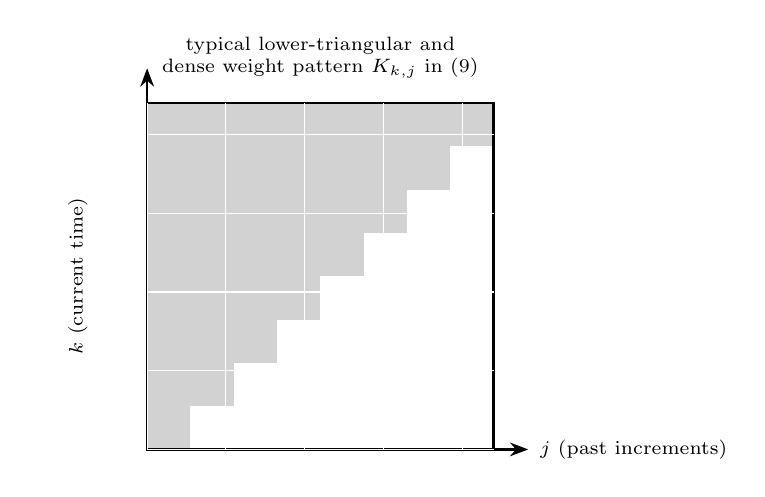
\begin{tikzpicture}[x=0.55cm,y=0.55cm,>=Stealth]

\def\n{8}

\foreach \k in {1,...,\n}{
  \foreach \j in {1,...,\n}{
    \ifnum\k<\j
      \fill[white] (\j-1,\k-1) rectangle (\j,\k);
    \else
      \fill[gray!35] (\j-1,\k-1) rectangle (\j,\k);
    \fi
  }
}

\draw[black, thick] (0,0) rectangle (\n,\n);
\draw[white!60] (0,0) grid (\n,\n);

\draw[->, thick] (0,\n) -- (0,\n+0.8);
\draw[->, thick] (\n,0) -- (\n+0.8,0);

\node[font=\scriptsize, rotate=90, anchor=south] at (-1.15,\n/2) {$k$ (current time)};
\node[font=\scriptsize, anchor=west] at (\n+0.85,0) {$j$ (past increments)};

\node[font=\scriptsize, align=center, text width=7.2cm]
at (\n/2,\n+1.05)
{typical lower-triangular and dense weight pattern $K_{k,j}$ in (9)};

\end{tikzpicture}
\caption{Schematic structure of the discretised Volterra weights $K_{k,j}$: each current value aggregates many past increments, creating dense temporal dependence and higher computational cost at fine time grids \cite{BayerFriz2016}.}
\label{fig:volterra_weights_structure}
\end{figure}
\FloatBarrier

\paragraph{Class I: direct Gaussian simulation via covariance and Cholesky.}
A straightforward approach is to discretise the relevant Gaussian vector, such as $(Y_1,\dots,Y_n)$, and sample it as a multivariate normal with a dense covariance matrix $\Sigma$. One then draws $Z\sim\mathcal{N}(0,I)$ and sets $Y=LZ$, where $LL^\top=\Sigma$ is a Cholesky factor, as described in \cite{BayerFriz2016}. While this method is robust and easy to implement, it becomes computationally expensive for large $n$ because $\Sigma$ is dense and factorisation costs increase rapidly with dimension, as noted in \cite{BayerFriz2016}. This dense-covariance challenge motivates the development of alternative schemes.

\begin{figure}[H]
\centering
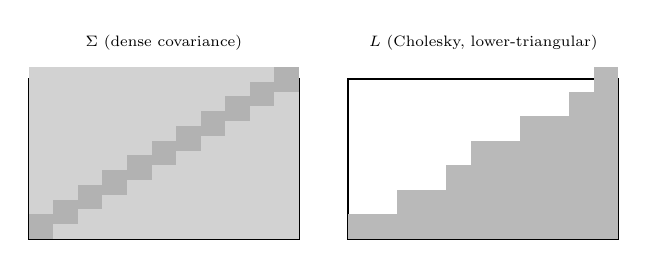
\begin{tikzpicture}[scale=0.78, every node/.style={transform shape}]
\begin{scope}
\node[font=\scriptsize] at (2.2,3.2) {$\Sigma$ (dense covariance)};
\draw[thick] (0,0) rectangle (4.4,2.6);
\foreach \i in {0,...,10}{
  \foreach \j in {0,...,6}{
    \fill[gray!35] (0.4*\i,0.4*\j) rectangle ++(0.4,0.4);
  }
}
\foreach \t in {0,...,10}{
  \fill[gray!60] (0.4*\t,0.4*\t*0.6) rectangle ++(0.4,0.4);
}
\end{scope}
\begin{scope}[xshift=5.2cm]
\node[font=\scriptsize] at (2.2,3.2) {$L$ (Cholesky, lower-triangular)};
\draw[thick] (0,0) rectangle (4.4,2.6);
\foreach \i in {0,...,10}{
  \foreach \j in {0,...,6}{
    \pgfmathsetmacro{\cond}{(\j <= 0.6*\i) ? 1 : 0}
    \ifnum\cond=1
      \fill[gray!55] (0.4*\i,0.4*\j) rectangle ++(0.4,0.4);
    \fi
  }
}
\end{scope}
\end{tikzpicture}
\caption{Illustration of the dense covariance matrix $\Sigma$ arising from discretised rough/Volterra drivers and its lower-triangular Cholesky factor $L$. Direct simulation samples $Y=LZ$, but the dense structure is a computational bottleneck at fine time grids \cite{BayerFriz2016}.}
\label{fig:covariance_cholesky_cartoon}
\end{figure}
\FloatBarrier

\paragraph{Class II: hybrid and convolution-based schemes.}
To reduce computational cost while maintaining accuracy near the kernel singularity, \cite{BayerFriz2016} introduces hybrid methods that treat near-diagonal (small-lag) contributions with higher fidelity and approximate the long-memory tail with coarser accuracy. At a high level, the sum in \eqref{eq:volterra_discrete_generic} is split into two parts:
\[
Y_k \approx \sum_{j=k-m}^{k-1} K_{k,j}\,\Delta W_j \;+\; \sum_{j=0}^{k-m-1} K_{k,j}\,\Delta W_j,
\]
where $m$ is a small window size. The first term captures the kernel's behaviour near zero, where rough kernels are most singular. The second term is approximated by leveraging the smoother behaviour at larger lags \cite{BayerFriz2016}. A practical approach is to interpret the long-memory part as a discrete convolution with a kernel and accelerate it using structured linear algebra or FFT-based techniques, as demonstrated in \cite{BayerFriz2016}. Notably, \cite{BayerFriz2016} highlights that exploiting correlation and structure to accelerate simulation is a key area for further research, providing a bridge from baseline methods to modern acceleration techniques.

\paragraph{Class III: approximations reducing memory and complexity.}
Another common approach is to approximate the non-Markovian driver using a higher-dimensional Markovian system, known as finite-dimensional state augmentation, or by using simpler surrogates for the covariance structure. The main goal is to reduce memory use and speed up each simulation path \cite{BayerFriz2016}. Numerically, these methods trade some model accuracy for faster performance. They focus on retaining the most important marginal and dependence features for pricing and hedging while enabling large-scale Monte Carlo simulations \cite{BayerFriz2016}.

\paragraph{Accuracy--speed trade-offs.}
The practical choice of a simulation scheme is governed by a trade-off between (i) accuracy of the rough driver at short time scales, (ii) computational complexity as the time grid is refined, and (iii) numerical stability under repeated Monte Carlo sampling \cite{BayerFriz2016}. The following schematic comparison summarises the main algorithmic ideas.

\begin{figure}[H]
\centering
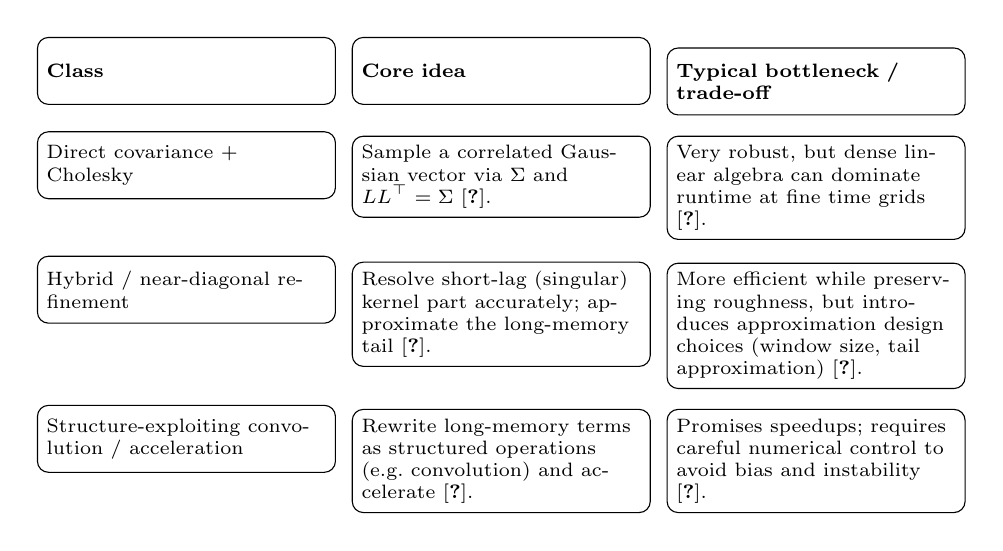
\begin{tikzpicture}[scale=0.88, every node/.style={transform shape, font=\scriptsize}]
\matrix (T) [matrix of nodes, nodes in empty cells,
nodes={draw, rounded corners, align=left, text width=3.55cm, minimum height=0.85cm},
column sep=2mm, row sep=2mm]{
\textbf{Class} &
\textbf{Core idea} &
\textbf{Typical bottleneck / trade-off} \\
Direct covariance + Cholesky &
Sample a correlated Gaussian vector via $\Sigma$ and $LL^\top=\Sigma$ \cite{BayerFriz2016}. &
Very robust, but dense linear algebra can dominate runtime at fine time grids \cite{BayerFriz2016}. \\
Hybrid / near-diagonal refinement &
Resolve short-lag (singular) kernel part accurately; approximate the long-memory tail \cite{BayerFriz2016}. &
More efficient while preserving roughness, but introduces approximation design choices (window size, tail approximation) \cite{BayerFriz2016}. \\
Structure-exploiting convolution / acceleration &
Rewrite long-memory terms as structured operations (e.g.\ convolution) and accelerate \cite{BayerFriz2016}. &
Promises speedups; requires careful numerical control to avoid bias and instability \cite{BayerFriz2016}. \\
};
\end{tikzpicture}
\caption{Schematic comparison of simulation scheme classes for rough/Volterra volatility drivers, highlighting typical computational bottlenecks and trade-offs \cite{BayerFriz2016}.}
\label{fig:scheme_comparison_table}
\end{figure}
\FloatBarrier

\paragraph{What matters for Monte Carlo in hedging.}
In hedging, simulation quality depends not only on pricing accuracy but also on the stability of the resulting hedging P\&L distribution, particularly in the tails targeted by convex objectives such as expected shortfall \cite{Buehler2019DeepHedging}. Deep hedging increases computational demands because training neural-network strategies requires repeated objective evaluations across many simulated paths and optimisation iterations, as described in \cite{Buehler2019DeepHedging,Horvath2021DeepRough}. As a result:
\begin{itemize}
\item \emph{Tail stability:} discretisation and sampling errors can distort rare-event behaviour and thus affect risk measures and learned strategies \cite{Buehler2019DeepHedging,BayerFriz2016}.
\item \emph{Reproducibility:} controlled random seeds, consistent dataset splits (train/validation/test), and fixed simulation protocols are essential to compare hedging methods fairly \cite{Buehler2019DeepHedging,Horvath2021DeepRough}.
\item \emph{Error control:} one must monitor both statistical error (finite $N$) and numerical bias (time discretisation, kernel approximation), since either can dominate in rough settings \cite{BayerFriz2016,Horvath2021DeepRough}.
\item \emph{Computational budget:} the overall cost must be compatible with large-scale Monte Carlo and repeated training runs, which motivates structure-exploiting and hybrid approaches beyond direct dense-covariance sampling \cite{Buehler2019DeepHedging,BayerFriz2016}.
\end{itemize}

\paragraph{Outlook and link to implementation.}
The previous discussion suggests that we should focus on simulation methods that keep short-term roughness but also use structural features to save time and memory \cite{BayerFriz2016}. In Section 5.3, we will describe a specific simulation method for the rough-volatility model used in our numerical experiments and explain our implementation choices and validation tests.

\subsection{Consequences for Hedging and Model Risk}
\label{subsec:consequences_hedging_model_risk}

This subsection discusses how rough volatility dynamics, such as Volterra-type models, significantly affect hedging errors and change the nature of model risk.
In particular, the usual idea that delta hedging becomes more accurate with frequent rebalancing does not hold when volatility is rough and shows strong short-term irregularity.
Because of these effects, there is a move away from analytical replication-based approaches toward risk-minimisation and learning-based hedging in incomplete, path-dependent markets \cite{BlackScholes1973,Heston1993,GatheralRough,BayerFriz2016,FoellmerSchied2016,Horvath2021DeepRough}

\paragraph{Model risk and a robustness benchmark.}
We interpret \emph{model risk} as the risk of adverse P\&L outcomes caused by using a misspecified dynamics to compute a trading rule (e.g.\ a delta computed under an assumed volatility model that differs from the data-generating one) \cite{ElKaroui1998Robustness,FoellmerSchied2016}
A useful benchmark is the ``robustness'' property of delta hedging in diffusion-type settings: hedging errors can often be expressed explicitly in terms of the discrepancy between the \emph{assumed} and \emph{realised} variance, and they vanish when this discrepancy vanishes \cite{ElKaroui1998Robustness,BlackScholes1973}

\begin{proposition}[A volatility-misspecification hedging-error identity (diffusion benchmark)]
\label{prop:delta_hedge_error_identity}
Let $S$ satisfy
\[
\frac{dS_t}{S_t} = \sigma_t\,dW_t, \qquad t\in[0,T],
\]
under a pricing measure, with an adapted volatility process $\sigma_t$.
Let $u(t,s;\bar\sigma)$ be the Black--Scholes price of a European payoff $g(S_T)$ computed with a \emph{constant} volatility parameter $\bar\sigma>0$, and let $\Delta_t := \partial_s u(t,S_t;\bar\sigma)$ be the corresponding delta strategy with continuous rebalancing and zero transaction costs.
Then the terminal replication error satisfies
\[
g(S_T) - u(0,S_0;\bar\sigma) - \int_0^T \Delta_t\,dS_t
=
\frac{1}{2}\int_0^T \Gamma_t\,S_t^2\bigl(\sigma_t^2-\bar\sigma^{\,2}\bigr)\,dt,
\]
where $\Gamma_t := \partial_{ss}u(t,S_t;\bar\sigma)$ is the Black--Scholes gamma.
\end{proposition}

\begin{proof}
Apply It\^o's formula to $u(t,S_t;\bar\sigma)$:
\[
du(t,S_t;\bar\sigma)
=
\partial_t u\,dt + \partial_s u\,dS_t + \frac{1}{2}\partial_{ss}u\,d\langle S\rangle_t.
\]
Since $d\langle S\rangle_t = S_t^2\sigma_t^2\,dt$ and $u$ solves the Black--Scholes PDE
\[
\partial_t u + \frac{1}{2}\bar\sigma^{\,2}s^2\partial_{ss}u = 0,
\]
we obtain
\[
du(t,S_t;\bar\sigma)
=
\Delta_t\,dS_t
+
\frac{1}{2}\Gamma_t S_t^2\bigl(\sigma_t^2-\bar\sigma^{\,2}\bigr)\,dt.
\]
Integrating from $0$ to $T$ and using $u(T,S_T;\bar\sigma)=g(S_T)$ yields the claim \cite{BlackScholes1973,ElKaroui1998Robustness}
\end{proof}

\begin{remark}[Interpretation: what ``robustness'' means here]\label{rem:robustness_meaning}
Proposition~\ref{prop:delta_hedge_error_identity} shows that, in a diffusion benchmark, the delta-hedging error depends on the difference between the realised instantaneous variance $\sigma_t^2$ and the model-implied variance $\bar\sigma^{\,2}$, with the option gamma acting as a weight.
This is why, in smooth situations, small mistakes in volatility estimates usually lead to manageable hedging errors. It also explains why many discussions about robustness focus on controlling realised variance or quadratic variation \cite{ElKaroui1998Robustness,BlackScholes1973}.
\end{remark}

\begin{figure}[H]
\centering
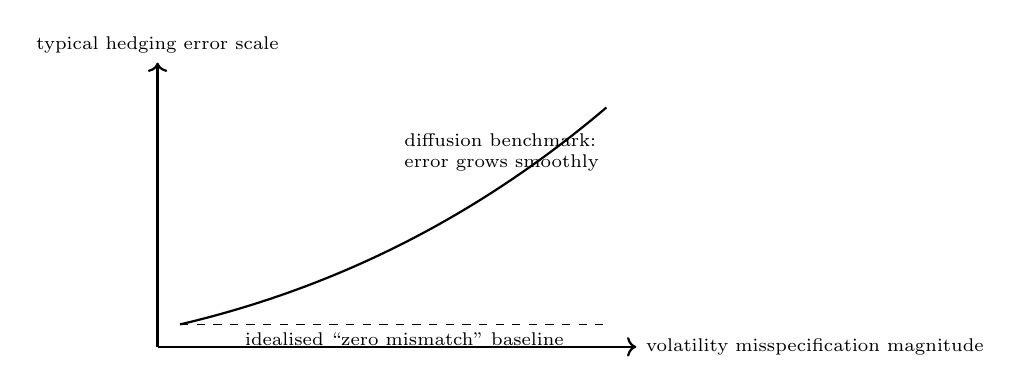
\begin{tikzpicture}[scale=0.95, every node/.style={transform shape}]
% axes
\draw[->, thick] (0,0) -- (6.4,0) node[right] {\scriptsize volatility misspecification magnitude};
\draw[->, thick] (0,0) -- (0,3.8) node[above] {\scriptsize typical hedging error scale};
% curves
\draw[thick] (0.3,0.3) .. controls (2.0,0.7) and (4.0,1.5) .. (6.0,3.2);
\node[font=\scriptsize, align=left] at (4.6,2.6) {diffusion benchmark:\\error grows smoothly};
% small annotation
\draw[dashed] (0.3,0.3) -- (6.0,0.3);
\node[font=\scriptsize] at (3.3,0.1) {idealised ``zero mismatch'' baseline};
\end{tikzpicture}
\caption{Schematic benchmark: under smooth diffusion assumptions, delta-hedging errors admit variance-mismatch representations (Proposition~\ref{prop:delta_hedge_error_identity}), which motivates a ``robustness'' intuition \cite{ElKaroui1998Robustness,BlackScholes1973}}
\label{fig:robustness_benchmark}
\end{figure}
\FloatBarrier

\paragraph{Why delta hedging breaks under rough volatility.}
Research on rough volatility shows that volatility, or log-volatility, is much more irregular over short time frames than classical diffusion models suggest. This irregularity matches scaling behaviour with Hurst indices $H\ll 1/2$ \cite{GatheralRough}.
This roughness leads to great high-frequency changes in $\sigma_t$ and makes gamma-weighted variance-mismatch terms unstable, especially close to maturity when gamma can be large \cite{GatheralRough,BayerFriz2016}.
Also, rough-volatility models are usually non-Markovian when using a small number of state variables. This means you cannot easily describe future variance dynamics using only the current volatility, which reduces the practical usefulness of delta rules from Markovian models like Black-Scholes or the standard Heston model \cite{Heston1993,GatheralRough,BayerFriz2016}.

\begin{remark}[From ``variance mismatch'' to ``tail risk'' in hedging P\&L]\label{rem:variance_to_tail}
Even if a variance-mismatch identity is available in a model (or as an approximation), roughness shifts the emphasis from mean error to \emph{tail behaviour}: short-term irregularity amplifies P\&L variability and can generate heavy-tailed hedging-loss distributions under discretisation and calibration error \cite{GatheralRough,BayerFriz2016,FoellmerSchied2016}
This tail-sensitivity is particularly relevant when the hedging objective is formulated via convex risk measures (e.g.\ entropic risk or expected shortfall), which explicitly penalise adverse tails \cite{FoellmerSchied2016,Buehler2019DeepHedging}
\end{remark}

\paragraph{Path dependence and roughness.}
A core difficulty for hedging under rough volatility is that volatility dynamics are typically \emph{non-Markovian}: future variance depends on the past through a Volterra-type structure, so a low-dimensional ``current state'' is not sufficient to describe the conditional law of future volatility \cite{GatheralRough,BayerFriz2016}. 
This history dependence should not be confused with \emph{long memory} in the sense of long-range dependence. In fractional models, long-range dependence is associated with $H>1/2$, whereas rough volatility is characterised by $H<1/2$ and reflects low short-term regularity rather than persistent correlations \cite{GatheralRough}. 
Accordingly, modelling log-volatility increments via fractional Brownian motion with $H\in(0,1/2)$ provides a parsimonious way to encode short-term roughness while retaining non-Markovian dependence \cite{GatheralRough}.

\begin{theorem}[Fractional Brownian motion is not Markov for $H\neq \tfrac{1}{2}$]
\label{thm:fbm_not_markov}
Let $W^H=\{W_t^H:t\ge0\}$ be fractional Brownian motion with Hurst parameter $H\in(0,1)$, i.e.\ a centred Gaussian process with covariance
\[
\mathbb{E}[W_t^H W_s^H] = \frac{1}{2}\Bigl(t^{2H}+s^{2H}-|t-s|^{2H}\Bigr).
\]
If $H\neq \tfrac{1}{2}$, then $W^H$ does not have the Markov property.
\end{theorem}

\begin{proof}
For a centred Gaussian process, the Markov property is equivalent to the conditional covariance identity
\[
\mathrm{Cov}(X_s,X_t\,|\,X_u)=0 \quad \text{for all } s<u<t,
\]
or, equivalently,
\[
\mathrm{Cov}(X_s,X_t) = \frac{\mathrm{Cov}(X_s,X_u)\,\mathrm{Cov}(X_u,X_t)}{\mathrm{Var}(X_u)}
\quad \text{for all } s<u<t.
\]
Apply this criterion to $X_t=W_t^H$. Fix $s=1$, $u=2$, $t=3$ (any strictly increasing triple works).
Let $C(a,b):=\mathbb{E}[W_a^H W_b^H]$.
Then
\[
C(1,3) = \frac{1}{2}\bigl(1^{2H}+3^{2H}-2^{2H}\bigr),
\qquad
C(1,2) = \frac{1}{2}\bigl(1^{2H}+2^{2H}-1^{2H}\bigr)=\frac{1}{2}2^{2H},
\]
\[
C(2,3)=\frac{1}{2}\bigl(2^{2H}+3^{2H}-1^{2H}\bigr),
\qquad
\mathrm{Var}(W_2^H)=C(2,2)=2^{2H}.
\]
If $W^H$ were Markov, we would have
\[
C(1,3) \stackrel{?}{=} \frac{C(1,2)\,C(2,3)}{C(2,2)}
= \frac{\bigl(\frac{1}{2}2^{2H}\bigr)\,C(2,3)}{2^{2H}}=\frac{1}{2}C(2,3)
=\frac{1}{4}\bigl(2^{2H}+3^{2H}-1\bigr).
\]
Comparing with $C(1,3)=\frac{1}{2}(1+3^{2H}-2^{2H})$, we obtain the equality condition
\[
\frac{1}{2}(1+3^{2H}-2^{2H})=\frac{1}{4}(2^{2H}+3^{2H}-1),
\]
which simplifies to
\[
2 + 2\cdot 3^{2H} - 2\cdot 2^{2H} = 2^{2H}+3^{2H}-1
\quad\Longleftrightarrow\quad
3 + 3^{2H} = 3\cdot 2^{2H}.
\]
This identity holds when $H=\tfrac{1}{2}$ (Brownian motion), but it fails for $H\neq\tfrac{1}{2}$ (e.g.\ one checks monotonicity of the function $H\mapsto 3+3^{2H}-3\cdot2^{2H}$ and notes it has a unique zero at $H=\tfrac{1}{2}$).

By the $H$-self-similarity of fractional Brownian motion,
\[
(W^H_{ct})_{t \geq 0} \stackrel{d}{=} (c^H W^H_t)_{t \geq 0} \qquad \text{for every } c > 0,
\]
the covariance satisfies $\mathrm{Cov}(W^H_{ca}, W^H_{cb}) = c^{2H}\,\mathrm{Cov}(W^H_a, W^H_b)$, so the scaling factors cancel in the Markov-criterion identity and the failure at $(1, 2, 3)$ transfers to every triple of the form $(c, 2c, 3c)$ with $c > 0$. Moreover, for a centred Gaussian process the failure of the conditional-covariance Markov criterion at any single triple $s < u < t$ is sufficient to conclude that the process does not possess the Markov property; see standard treatments of Gaussian Markov processes.

Hence the Markov criterion fails, so $W^H$ is not Markov for $H\neq\tfrac{1}{2}$ \cite{GatheralRough}.
\end{proof}

\begin{remark}[Hedging implication: ``state compression'' is intrinsically lossy]\label{rem:state_compression_lossy}
Theorem~\ref{thm:fbm_not_markov} explains why roughness usually leads to path dependence. When volatility drivers act like $H\ll 1/2$ fBm-type processes, it is not possible for any finite-dimensional Markov state based only on the current volatility level to capture the full conditional distribution of future volatility (\cite{GatheralRough,BayerFriz2016}).
For hedging, this implies that strategies based only on $(t,S_t,v_t)$ are structurally misspecified in these settings. This creates a direct source of model risk \cite{Heston1993,GatheralRough,FoellmerSchied2016}.
\end{remark}

\begin{figure}[H]
\centering
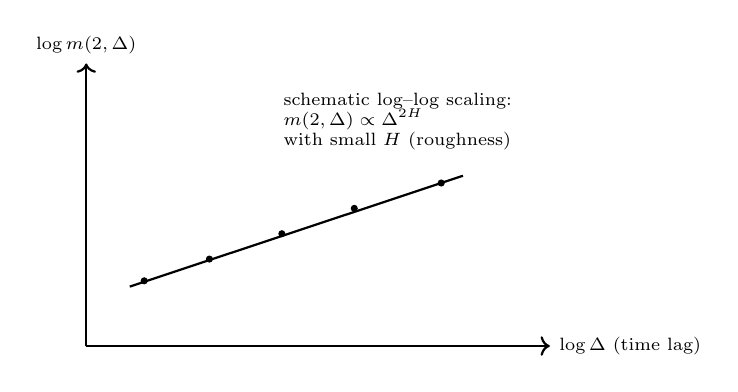
\begin{tikzpicture}[scale=0.92, every node/.style={transform shape}]
% axes
\draw[->, thick] (0,0) -- (6.4,0) node[right] {\scriptsize $\log \Delta$ (time lag)};
\draw[->, thick] (0,0) -- (0,3.9) node[above] {\scriptsize $\log m(2,\Delta)$};
% points roughly on a line with small slope (~2H)
\fill (0.8,0.9) circle (1.4pt);
\fill (1.7,1.2) circle (1.4pt);
\fill (2.7,1.55) circle (1.4pt);
\fill (3.7,1.9) circle (1.4pt);
\fill (4.9,2.25) circle (1.4pt);
% fitted line
\draw[thick] (0.6,0.82) -- (5.2,2.35);
\node[font=\scriptsize, align=left] at (4.3,3.1)
{schematic log--log scaling:\\$m(2,\Delta)\propto \Delta^{2H}$\\with small $H$ (roughness)};
\end{tikzpicture}
\caption{Schematic reproduction of the empirical log--log scaling used to infer roughness from realised-volatility proxies, where a small slope corresponds to $H\ll \tfrac{1}{2}$ \cite{GatheralRough}}
\label{fig:roughness_scaling_schematic}
\end{figure}
\FloatBarrier

\paragraph{Motivation for learning-based strategies (risk minimisation).}
In markets that are rough, incomplete, and path-dependent, replication is usually not possible. Instead, hedging is typically framed as minimising a risk functional of terminal P\&L \cite{FoellmerSchied2016}.
Convex risk measures offer a consistent mathematical approach to capture tail aversion. They define the optimal hedge as the solution to an optimisation problem with constraints, rather than relying on replication \cite{FoellmerSchied2016,Buehler2019DeepHedging}.
This approach aligns with the deep-hedging paradigm. In this framework, trading rules are parameterised, for example by neural networks, and trained to minimise empirical convex-risk objectives on simulated paths \cite{Buehler2019DeepHedging}.

\begin{proposition}[From replication to risk-minimising hedging in incomplete markets]
\label{prop:replication_to_risk_min}
In a discrete-time market with frictions and constraints, the set of attainable terminal gains is typically non-linear and does not allow exact replication of a general liability.
Let $\rho$ be a convex risk measure on terminal P\&L and let $X$ be a liability.
Then an optimal hedge is naturally defined as any minimiser of
\[
\inf_{\delta\in\mathcal H}\rho\bigl(-X + (\delta\cdot S)_T - C_T(\delta)\bigr),
\]
and the associated value is a (cash-invariant) risk-based capital requirement. 
\end{proposition}

\begin{proof}
See Appendix~\ref{app:proofs}, Proof of Proposition~\ref{prop:replication_to_risk_min}.
\end{proof}

\begin{remark}[Why this connects directly to deep hedging under rough volatility]\label{rem:deep_hedging_connection}
The optimisation viewpoint in Proposition~\ref{prop:replication_to_risk_min} is precisely what enables learning-based strategies: once the objective is a risk functional of terminal P\&L, one can optimise over a rich parametrised class of strategies (e.g.\ neural networks) and compute gradients by backpropagation and stochastic-gradient methods \cite{Buehler2019DeepHedging,HighamHigham2019DeepLearning}
This is particularly attractive in rough-volatility environments, where the underlying drivers are non-Markovian and path dependent, and where classical Greek-based hedging becomes unstable \cite{GatheralRough,BayerFriz2016,Horvath2021DeepRough}
\end{remark}

\begin{figure}[H]
\centering
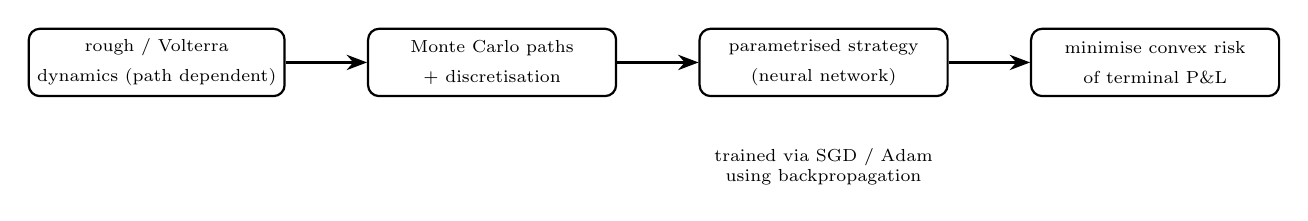
\begin{tikzpicture}[
    scale=0.9,
    every node/.style={transform shape},
    box/.style={draw, thick, rounded corners, minimum width=3.5cm, minimum height=0.95cm, align=center},
    arr/.style={-{Stealth[length=2.6mm]}, thick},
    node distance=1.15cm
]
\node[box] (rv) {\scriptsize rough / Volterra\\ \scriptsize dynamics (path dependent)};
\node[box, right=of rv] (mc) {\scriptsize Monte Carlo paths\\ \scriptsize + discretisation};
\node[box, right=of mc] (nn) {\scriptsize parametrised strategy\\ \scriptsize (neural network)};
\node[box, right=of nn] (risk) {\scriptsize minimise convex risk\\ \scriptsize of terminal P\&L};

\draw[arr] (rv) -- (mc);
\draw[arr] (mc) -- (nn);
\draw[arr] (nn) -- (risk);

\node[below=6mm of nn, font=\scriptsize, align=center]
{trained via SGD / Adam\\using backpropagation};
\end{tikzpicture}
\caption{Bridge from rough path dependence to learning-based hedging: non-Markovian dynamics motivate a risk-minimisation formulation and optimisation over rich strategy classes \cite{FoellmerSchied2016,Buehler2019DeepHedging,Horvath2021DeepRough}}
\label{fig:bridge_to_deep_hedging}
\end{figure}
\FloatBarrier

\paragraph{Bridge to the next chapter (Hedging Frameworks).}
The remainder of this dissertation operationalises the consequences above by comparing hedging rules in controlled simulations.
Section~4.1 (Delta Hedging) implements classical delta-based strategies computed under potentially misspecified volatility models and studies how roughness and discretisation affect realised P\&L and its tails \cite{BlackScholes1973,Heston1993,GatheralRough}
Section~4.2 (Deep Hedging) follows the risk-minimisation paradigm: strategies are learned from simulated paths by minimising convex risk measures, with a particular focus on robustness to path dependence and rough volatility effects \cite{Buehler2019DeepHedging,Horvath2021DeepRough,FoellmerSchied2016}

\newpage

\section{Hedging Frameworks}
\label{sec:hedging_frameworks}

\noindent
This section explains hedging strategies and outlines a fixed protocol for comparison.
The aim is to create a single experimental setup in which both classical delta hedging and deep hedging are tested using the same trading rules, costs, and information. This way, any performance differences come from the hedging methods themselves, not from different assumptions or data.

\medskip

\begin{definition}[Comparison protocol: traded universe and liability]
\label{def:comparison_universe}
Throughout Section~\ref{sec:hedging_frameworks} and all numerical experiments, the hedger trades only in the underlying asset.
That is, the \emph{traded universe} consists of a single instrument with (discounted) mid-price process
\[
S_k := S_{t_k}, \qquad k=0,\dots,n,
\]
so that portfolio positions are scalar,
\[
\delta_k \in \mathbb{R}, \qquad k=0,\dots,n-1.
\]
The \emph{hedged liability} is a European contingent claim with discounted payoff
\[
Z = g(S_T),
\]
for a fixed measurable payoff function $g$ and maturity $T=t_n$.
\end{definition}

\begin{remark}[Why only the underlying is traded]
\label{rem:only_underlying}
Restricting hedging activities to the underlying asset isolates the effects of rough volatility, discretisation, and model misspecification on overall hedging performance.
Incorporating additional hedging instruments, such as vanilla options or variance swaps, alters both market completeness and the informational structure of the trading set. This introduces further modelling choices and calibration requirements, which may obscure a clear comparison between delta hedging and learning-based strategies.
\end{remark}

\begin{definition}[Comparison protocol: trading grid]
\label{def:comparison_grid}
All strategies are evaluated on the same deterministic \emph{trading grid}
\[
0=t_0 < t_1 < \cdots < t_n = T.
\]
Trading is allowed only at the grid times $t_k$.
A strategy $\delta=(\delta_k)_{k=0}^{n-1}$ holds position $\delta_k$ over the interval $[t_k,t_{k+1})$.
\end{definition}

\begin{remark}[Fairness and the role of rebalancing frequency]
\label{rem:grid_fairness}
The number of rebalancing dates $n$ (equivalently, the mesh size of the grid) is an experimental control variable.
However, for any fixed experiment, \emph{all} methods (delta hedging and deep hedging) use the \emph{same} grid as specified in Definition~\ref{def:comparison_grid}.
This ensures that differences in performance are not driven by differing trading opportunities.
\end{remark}

\begin{definition}[Comparison protocol: costs and constraints]
\label{def:comparison_costs_constraints}
Transaction costs and trading constraints are imposed exactly as in the discrete-time framework of Section~\ref{subsec:discrete_time_setting}.
In all experiments we fix a single cost specification and apply it uniformly across strategies.
In particular, we use proportional \emph{transaction costs} of the form
\[
c_k(\Delta \delta_k) = \lambda\, S_{t_k}\, |\Delta \delta_k|,
\qquad
\Delta \delta_k := \delta_k - \delta_{k-1},
\qquad
k=0,\dots,n,
\]
with a fixed coefficient $\lambda\ge 0$ and the convention $\delta_{-1}=\delta_n=0$.
If position constraints are imposed, they take the form
\[
\delta_k \in [\delta_{\min},\delta_{\max}]
\qquad\text{for all } k,
\]
and are enforced identically for all strategies.
\end{definition}

\begin{remark}[No redefinition of frictions]
\label{rem:no_redefine_frictions}
Definition~\ref{def:comparison_costs_constraints} sets the specific frictions used in the experiment for comparison.
The general admissibility and cost framework is given in Definitions~\ref{def:trading_strategy}--\ref{def:terminal_PL}; here we only specify the particular instance used consistently across all numerical results.
\end{remark}

\begin{definition}[Comparison protocol: information set]
\label{def:comparison_information}
Let $I_k$ denote the information available to the hedger at time $t_k$.
To ensure a fair comparison, we fix a common \emph{information set} shared by all strategies.
In this dissertation we take
\[
I_k := \bigl(t_k,\; S_{t_k},\; \tau_k,\; \delta_{k-1}\bigr),
\qquad
\tau_k := T-t_k,
\qquad
k=0,\dots,n-1.
\]
A hedging strategy is required to be predictable with respect to $(\mathcal{F}_k)_{k=0}^n$ and to satisfy
\[
\delta_k = f_k(I_k)
\quad\text{for some measurable map } f_k:\mathbb{R}^4\to\mathbb{R}.
\]
\end{definition}

\begin{remark}[Fairness principle: equal information]
\label{rem:fairness_equal_information}
Definition~\ref{def:comparison_information} is the key fairness constraint of the comparison protocol.
Both delta hedging and deep hedging observe the same features $I_k$ (spot, time, time-to-maturity, and previous position).
In particular, neither method observes latent volatility states of the data-generating model.
The only additional ingredient used by delta hedging is an \emph{assumed-model pricing/Greek engine} (e.g.\ Black--Scholes or Heston) used to compute $\Delta^{\mathrm{assumed}}(t_k,S_{t_k};\hat\theta)$ from the same inputs.
\end{remark}

\begin{definition}[Feature map for numerical implementation]
\label{def:feature-map}
For the numerical experiments in Section~\ref{sec:numerical_experiments}, we define a feature map
$\phi\colon \mathcal{I}_k \to \mathbb{R}^{d_\phi}$ applied to the information
set $I_k$ from Definition~\ref{def:comparison_information}. We consider the following
feature sets:
\begin{itemize}
  \item \textbf{Feature set~B} ($d_\phi = 3$): $\phi^B(I_k) = (t_k / T,\;
        \log(S_{t_k}/S_0),\; \tau_k / T)$. The previous hedge position~$\delta_{k-1}$ is
        appended to the network input in the rollout procedure, giving a
        total input dimension of~$4$. Since $S_0 = K$ in our baseline calibration (at-the-money call at $t = 0$), the two feature definitions $\log(S_{t_k}/K)$ and $\log(S_{t_k}/S_0)$ coincide exactly at every path point; we adopt $\log(S_{t_k}/S_0)$ in the numerical implementation because the reference to the trajectory's starting point is more natural for a path-centred feature.
  \item \textbf{Feature set~C} ($d_\phi = 4$): $\phi^C(I_k) = (\tau_k / T,\;
        \log(S_{t_k}/K),\; r_{k-1},\; \widehat{\sigma}^{\mathrm{RV}}_k)$,
        where $r_{k-1} = \log(S_{t_k}/S_{t_{k-1}})$ is the last observed
        log-return and $\widehat{\sigma}^{\mathrm{RV}}_k$ is a running
        realised-volatility estimate.
  \item \textbf{Feature set~D} ($d_\phi = 3$): $\phi^D(I_k) = (\tau_k / T,\;
        \log(S_{t_k}/K),\; \sigma_{\mathrm{in}})$, where $\sigma_{\mathrm{in}}$
        is an externally supplied volatility input.
\end{itemize}
All features are normalised to zero mean and unit standard deviation
using statistics computed on the training set only; the fitted normalisation
constants are saved and applied identically to validation and test sets.
\end{definition}

\begin{remark}[Information equivalence]\label{rem:information_equivalence}
Feature set~B is an invertible transformation of $(t_k, S_{t_k})$
for fixed~$T$ and~$K$: given $\tau_k/T$ and $\log(S_{t_k}/K)$ one recovers
$t_k = T(1 - \tau_k/T)$ and $S_{t_k} = K \exp(\log(S_{t_k}/K))$.
Consequently, the expressive power of the network is unchanged, but
normalised features improve gradient conditioning and training stability.
The redundant inclusion of both~$t_k$ and~$\tau_k$ from
Definition~\ref{def:comparison_information} is collapsed into the single
normalised quantity $\tau_k/T$, since $t_k + \tau_k = T$.
\end{remark}

\begin{definition}[Comparison protocol: reported performance criteria]
\label{def:comparison_metrics}
For a fixed liability $Z=g(S_T)$, initial capital $p_0$, and admissible strategy $\delta$, the performance object is the terminal profit-and-loss
\[
\mathrm{PL}_T(Z,p_0,\delta)
=
-\,Z + p_0 + \sum_{k=0}^{n-1} \delta_k\,(S_{t_{k+1}}-S_{t_k}) - C_T(\delta),
\]
as defined in Definition~\ref{def:terminal_PL}.
The comparison between hedging methods is based on:
\begin{enumerate}
\item the empirical distribution of $\mathrm{PL}_T$ (summary statistics and tail diagnostics);
\item risk measures of $\mathrm{PL}_T$, in particular Value-at-Risk and Expected Shortfall at levels $\alpha\in(0,1)$, and the entropic risk measure for fixed risk aversion $\lambda>0$ (as reviewed in Section~\ref{subsec:convex_risk_measures}).
\end{enumerate}
\end{definition}

\begin{remark}[Protocol vs.\ results]
\label{rem:protocol_vs_results}
Definition~\ref{def:comparison_metrics} specifies \emph{what} is reported, not \emph{how well} a method performs.
All numerical values, plots, and comparisons are deferred to Sections~\ref{sec:numerical_experiments} and~6--7.
\end{remark}

\medskip

\noindent
With the comparison protocol fixed, we can now define the concrete strategies.
Section~4.1 specifies the delta-hedging rules (including the assumed model family and parameter policy), and Section~4.2 specifies the deep-hedging strategy class and training objective.

\subsection{Sources of Model Risk and Experimental Axes}
\label{subsec:model_risk_axes}

\noindent
This subsection turns Section~\ref{sec:hedging_frameworks} into an explicit \emph{map of experiments}:
it defines the ``true world'' (data-generating dynamics), the ``assumed world'' (used to compute delta hedges),
and the ``training world'' (used to generate training paths for deep hedging). The numerical design in
Sections~\ref{sec:numerical_experiments}--7 is then organised along a small number of \emph{model-risk axes}
that isolate where misspecification enters the hedging pipeline \cite{GatheralRough,BayerFriz2016,BlackScholes1973,Heston1993,Buehler2019DeepHedging,Horvath2021DeepRough}

\begin{definition}[True vs.\ assumed vs.\ training world]
\label{def:true_assumed_training_worlds}
Fix the comparison protocol of Definitions~\ref{def:comparison_universe}--\ref{def:comparison_metrics}.
We distinguish three modelling layers:

\begin{enumerate}
\item \textbf{True (data-generating) model.}
The spot process $(S_t)_{t\in[0,T]}$ is generated under a \emph{rough volatility} model
\[
\mathcal{M}^{\mathrm{true}} := \mathcal{M}^{\mathrm{rBergomi}},
\]
as introduced in Section~\ref{sec:rough_volatility} (rough Bergomi) \cite{GatheralRough,BayerFriz2016}

\item \textbf{Assumed model (delta engine).}
Delta hedging is computed under an \emph{assumed} diffusion family
\[
\mathcal{M}^{\mathrm{ass}} \in \{\mathcal{M}^{\mathrm{BS}},\,\mathcal{M}^{\mathrm{Heston}}\},
\]
i.e.\ Black--Scholes or Heston, with parameter input $\hat\theta^{\mathrm{ass}}$ \cite{BlackScholes1973,Heston1993}

\item \textbf{Training model (deep hedging simulator).}
Deep hedging is trained on simulated paths from a model
\[
\mathcal{M}^{\mathrm{train}} \in \{\mathcal{M}^{\mathrm{true}},\,\text{controlled variants of }\mathcal{M}^{\mathrm{true}}\},
\]
with training parameters $\hat\theta^{\mathrm{train}}$.
This choice is treated as an explicit experimental factor controlling \emph{training misspecification} \cite{Buehler2019DeepHedging,Horvath2021DeepRough}
\end{enumerate}
\end{definition}

\begin{remark}[Why three ``worlds'' are necessary]
\label{rem:three_worlds}
By separating the elements in Definition~\ref{def:true_assumed_training_worlds}, we can identify three different effects:
(i) structural error in the analytical delta engine, such as differences between diffusion and rough volatility \cite{GatheralRough,BayerFriz2016}
(ii) parameter error within a chosen model family, such as calibration or estimation noise \cite{ElKaroui1998Robustness} and
(iii) learning error that happens when the network is trained on a simulator which might differ from the true dynamics \cite{Buehler2019DeepHedging,Horvath2021DeepRough}
\end{remark}

\medskip

\noindent
We now list the main \emph{axes of model risk} used to structure Section~\ref{sec:numerical_experiments}.

\begin{definition}[Axis I: structural misspecification (model class)]
\label{def:axis_structural}
\emph{Structural misspecification} refers to the case where the true dynamics are not contained in the assumed model family used for delta hedging:
\[
\mathcal{M}^{\mathrm{true}} \notin \mathcal{M}^{\mathrm{ass}}.
\]
In this dissertation the canonical structural mismatch is
\[
\mathcal{M}^{\mathrm{true}}=\mathcal{M}^{\mathrm{rBergomi}
}\quad\text{vs.}\quad
\mathcal{M}^{\mathrm{ass}}\in\{\mathcal{M}^{\mathrm{BS}},\mathcal{M}^{\mathrm{Heston}}\},
\]
i.e.\ rough, non-Markovian volatility drivers versus classical diffusion-based pricing engines \cite{GatheralRough,BayerFriz2016,BlackScholes1973,Heston1993}
\end{definition}

\begin{definition}[Axis II: parameter misspecification (within a fixed family)]
\label{def:axis_parameter}
\emph{Parameter misspecification} occurs when the parameter input used by a method differs from the relevant ``oracle'' parameter in the chosen family.
For delta hedging this takes the form
\[
\hat\theta^{\mathrm{ass}} \neq \theta^{\mathrm{ass}}_{\star},
\]
where $\theta^{\mathrm{ass}}_{\star}$ denotes a reference parameter choice for the assumed family
(e.g.\ a calibration target under the assumed model, or a controlled baseline used to generate sensitivity perturbations) \cite{ElKaroui1998Robustness}

For deep hedging, parameter misspecification can arise in training:
\[
\hat\theta^{\mathrm{train}} \neq \theta^{\mathrm{train}}_{\star},
\]
leading to a deliberate gap between training and deployment distributions \cite{Buehler2019DeepHedging,Horvath2021DeepRough}
\end{definition}

\begin{definition}[Axis III: discretisation and trading frictions]
\label{def:axis_discretisation_costs}
\emph{Discretisation and frictions} refer to the fact that hedging is implemented on a finite grid
(Definition~\ref{def:comparison_grid}) and incurs transaction costs / constraints (Definition~\ref{def:comparison_costs_constraints}).
This axis is controlled by:
\begin{itemize}
\item the rebalancing frequency (grid size $n$ / mesh), and
\item the friction level (e.g.\ proportional cost coefficient $\lambda$ and any bounds $[\delta_{\min},\delta_{\max}]$).
\end{itemize}
These effects are central in discrete-time hedging formulations and materially impact tail risk \cite{Buehler2019DeepHedging,FoellmerSchied2016,WhalleyWilmott2002}
\end{definition}

\begin{definition}[Axis IV: path dependence and state compression]
\label{def:axis_state_compression}
\emph{Path dependence / state compression} captures the information mismatch induced by non-Markovian volatility dynamics.
In rough/Volterra models, future volatility depends on a long history of past shocks, so any hedging rule using only a low-dimensional state
(e.g.\ $(t_k,S_{t_k})$ or $(t_k,S_{t_k},v_{t_k})$) is intrinsically compressing information \cite{GatheralRough,BayerFriz2016}

In the present protocol, classical delta hedges are of the form
\[
\delta_k = \Delta^{\mathrm{ass}}(t_k,S_{t_k};\hat\theta^{\mathrm{ass}}),
\]
which is (by construction) a Markovian decision rule in the observed spot/time variables \cite{BlackScholes1973,Heston1993}

Deep hedging, by contrast, is allowed to represent non-linear decision rules in the fixed information set $I_k$ (Definition~\ref{def:comparison_information}),
and can incorporate limited history through engineered features and/or the previous position $\delta_{k-1}$ \cite{Buehler2019DeepHedging,Horvath2021DeepRough}
\end{definition}

\begin{remark}[Fairness and what ``history'' means here]
\label{rem:history_fairness}
Axis~IV does \emph{not} give deep hedging privileged access to latent volatility.
It only reflects that a learning-based rule can approximate complex (potentially path-dependent) maps of the admissible feature set $I_k$,
whereas a delta hedge is constrained to the functional form imposed by the assumed model family \cite{Buehler2019DeepHedging,Horvath2021DeepRough,BlackScholes1973,Heston1993}
\end{remark}

\medskip

\noindent
The following table provides a compact ``where does this enter?'' view, which will be used as the organising backbone of Section~\ref{sec:numerical_experiments}.

\begin{table}[H]
\centering
\caption{Model-risk axes used to organise Section~\ref{sec:numerical_experiments} and where they enter the hedging pipeline (logical map; no numerical values).}
\label{tab:model_risk_axes_map}
\renewcommand{\arraystretch}{1.15}
\begin{tabular}{p{3.4cm} p{6.2cm} p{5.2cm}}
\toprule
\textbf{Axis} & \textbf{Where it enters (definition-level)} & \textbf{Primary effect / what it stresses} \\
\midrule
(I) Structural misspecification &
Mismatch $\mathcal{M}^{\mathrm{true}}$ vs.\ $\mathcal{M}^{\mathrm{ass}}$ (diffusion delta engine under rough true dynamics) \cite{GatheralRough,BayerFriz2016,BlackScholes1973,Heston1993}
&
Systematic hedging bias and unstable short-horizon behaviour under roughness; isolates ``wrong model class'' risk \cite{GatheralRough,BayerFriz2016} \\
\addlinespace
(II) Parameter misspecification &
Inputs $\hat\theta^{\mathrm{ass}}$ (delta) and/or $\hat\theta^{\mathrm{train}}$ (training simulator) differ from reference baselines \cite{ElKaroui1998Robustness,Buehler2019DeepHedging,Horvath2021DeepRough}
&
Sensitivity to calibration/estimation error; stress-tests robustness to perturbations without changing the model class \cite{ElKaroui1998Robustness} \\
\addlinespace
(III) Discretisation + costs &
Common trading grid $0=t_0<\dots<t_n=T$ and cost functional $c_k(\cdot)$, with controls $(n,\lambda,[\delta_{\min},\delta_{\max}])$ \cite{Buehler2019DeepHedging,FoellmerSchied2016,WhalleyWilmott2002}
&
Tail risk and replication error from discrete trading; reveals speed--accuracy and friction sensitivity across methods \cite{FoellmerSchied2016,Buehler2019DeepHedging} \\
\addlinespace
(IV) Path dependence / state compression &
True model is non-Markovian; delta rule is Markovian in $(t_k,S_{t_k})$; deep hedge approximates flexible maps of $I_k$ including $\delta_{k-1}$ \cite{GatheralRough,BayerFriz2016,Buehler2019DeepHedging,Horvath2021DeepRough}
&
Measures how much performance is lost by compressing history into a low-dimensional state; motivates learning-based rules under rough volatility \cite{GatheralRough,Horvath2021DeepRough} \\
\bottomrule
\end{tabular}
\end{table}

\begin{remark}[How this becomes the experimental ``roadmap'']
\label{rem:roadmap_sections_6_7}
Section~\ref{sec:numerical_experiments} will change these factors in a controlled way:
structural misspecification by switching the delta engine (BS vs.\ Heston) under a fixed rough true model \cite{BlackScholes1973,Heston1993,BayerFriz2016}
parameter misspecification by perturbing $\hat\theta^{\mathrm{ass}}$ and/or $\hat\theta^{\mathrm{train}}$ \cite{ElKaroui1998Robustness,Horvath2021DeepRough}
discretisation and costs by varying $(n,\lambda)$ \cite{WhalleyWilmott2002,Buehler2019DeepHedging}
and state compression by comparing Markovian delta rules against learned strategies defined on the fixed feature set $I_k$ \cite{Buehler2019DeepHedging,Horvath2021DeepRough}
\end{remark}

\subsection{Delta Hedging}
\label{subsec:delta_hedging}

\noindent
This subsection clearly defines what “delta” means in our experiments and explains where model misspecification occurs.
We consider two delta engines: Black--Scholes and Heston \cite{BlackScholes1973,Heston1993}

\label{subsubsec:delta_definition}

\begin{definition}[Discrete-time delta hedging rule under an assumed model]
\label{def:delta_strategy_assumed}
Fix an assumed model family $\mathcal{M}^{\mathrm{ass}}$ and an assumed parameter input $\hat\theta^{\mathrm{ass}}$.
Let $u^{\mathrm{ass}}(t,s;\hat\theta^{\mathrm{ass}})$ denote the corresponding model price (at time $t$ and spot $s$)
of the European payoff $Z=g(S_T)$.
The \emph{assumed-model delta} is defined by
\[
\Delta^{\mathrm{ass}}(t,s;\hat\theta^{\mathrm{ass}}) := \partial_s u^{\mathrm{ass}}(t,s;\hat\theta^{\mathrm{ass}}).
\]
The corresponding \emph{discrete-time delta hedging strategy} is
\begin{equation}
\label{eq:delta_discrete_strategy}
\delta^{\Delta}_k
:=
\Delta^{\mathrm{ass}}(t_k,S_{t_k};\hat\theta^{\mathrm{ass}}),
\qquad k=0,\dots,n-1,
\end{equation}
implemented on the common grid from Definition~\ref{def:comparison_grid} \cite{BlackScholes1973,Heston1993}
\end{definition}

\begin{remark}[Discrete rebalancing and transaction costs]
\label{rem:delta_discrete_rebalancing_costs}
The position $\delta_k^\Delta$ is held over $[t_k,t_{k+1})$ and updated only at grid times.
Transaction costs are included at each update using a standard cost function.
$c_k(\delta_k-\delta_{k-1})$ fixed in Definition~\ref{def:comparison_costs_constraints},
with the conventions $\delta_{-1}=\delta_n=0$ and $c_k(0)=0$ \cite{Buehler2019DeepHedging}
\end{remark}

\begin{remark}[Where misspecification enters for delta hedging]
\label{rem:where_misspec_enters_delta}
Delta hedging uses an assumed pricing map $u^{\mathrm{ass}}$ and its spot derivative.
Model risk enters through:
(i) the \emph{functional form} of $u^{\mathrm{ass}}$ (Axis I, structural misspecification),
(ii) the parameter input $\hat\theta^{\mathrm{ass}}$ (Axis II, parameter misspecification),
and (iii) discrete rebalancing with costs (Axis III) \cite{ElKaroui1998Robustness,BlackScholes1973,Heston1993,Buehler2019DeepHedging}
\end{remark}

\subsubsection{Variant A: Black--Scholes delta}
\label{subsubsec:bs_delta}

\begin{definition}[Assumed model: Black--Scholes price and delta]
\label{def:bs_price_delta}
In the Black--Scholes assumed model, the option price at time $t$ and spot $s$ is denoted
\[
u^{\mathrm{BS}}(t,s;\bar\sigma),
\]
where the (only) model parameter is the constant volatility input $\hat\theta^{\mathrm{ass}}=\bar\sigma>0$ \cite{BlackScholes1973}
The Black--Scholes delta is
\[
\Delta^{\mathrm{BS}}(t,s;\bar\sigma) := \partial_s u^{\mathrm{BS}}(t,s;\bar\sigma),
\]
and the associated delta strategy is
\[
\delta^{\Delta,\mathrm{BS}}_k := \Delta^{\mathrm{BS}}(t_k,S_{t_k};\bar\sigma), \qquad k=0,\dots,n-1.
\]
\end{definition}

\begin{remark}[Closed-form vs.\ derivative definition]
\label{rem:bs_closed_form}
For vanilla calls/puts, $\Delta^{\mathrm{BS}}$ admits the usual closed form;
nevertheless, for consistency across payoffs we regard delta as $\partial_s u^{\mathrm{BS}}$
and implement it as needed (analytically when available, otherwise via the same pricing engine) \cite{BlackScholes1973}
\end{remark}

\subsubsection{Variant B: Heston PDE delta}
\label{subsubsec:heston_delta}

\begin{definition}[Assumed model: Heston PDE price and delta]
\label{def:heston_pde_delta}
In the Heston assumed model of Definition~\ref{def:markovian_dynamics}(b),
the option price at time $t$, spot $s$, and instantaneous variance $v$ is
denoted
\[
u^{\mathrm{Hes}}(t, s, v;\hat\theta_{\mathrm{Hes}}),
\]
where the parameter vector is
$\hat\theta_{\mathrm{Hes}} = (\kappa, \theta, \sigma_v, \rho, V_0)$
\cite{Heston1993}. The Heston PDE delta is
\[
\Delta^{\mathrm{Hes}}(t, s, v;\hat\theta_{\mathrm{Hes}})
:= \partial_s u^{\mathrm{Hes}}(t, s, v;\hat\theta_{\mathrm{Hes}}),
\]
and the associated delta strategy is
\[
\delta_k^{\Delta, \mathrm{Hes}}
:= \Delta^{\mathrm{Hes}}\!\left(t_k, S_{t_k}, V_{t_k};
\hat\theta_{\mathrm{Hes}}\right),
\qquad k = 0, \ldots, n-1.
\]
\end{definition}

\begin{remark}[Numerical implementation and information access]
\label{rem:heston_pde_delta_implementation}
The Heston price function $u^{\mathrm{Hes}}$ does not admit a closed form
suitable for spot differentiation; we compute it on a grid by solving the
two-dimensional Heston pricing PDE numerically with a Hundsdorfer--Verwer
ADI scheme \cite{HundsdorferVerwer2003}, and extract the delta by central
differencing in $s$. The resulting $\Delta^{\mathrm{Hes}}$ depends on the
instantaneous variance $V_{t_k}$, which the Heston hedger observes;
calibration of $\hat\theta_{\mathrm{Hes}}$ is performed at the dissertation
calibration point and is detailed in Section~\ref{sec:6_3_1}.
\end{remark}

\label{subsubsec:delta_calibration_policy}

\begin{definition}[Baseline parameter policy (controlled, calibration-free)]
\label{def:baseline_param_policy}
In baseline experiments (Section~\ref{sec:numerical_experiments}), the assumed-model parameters
$\hat\theta^{\mathrm{ass}}$ are fixed \emph{a priori} (controlled inputs) and kept constant across all Monte Carlo paths.
This isolates structural misspecification (Axis I) and discretisation/friction effects (Axis III) without introducing an additional calibration layer.
Parameter misspecification (Axis II) is then studied separately in sensitivity experiments by perturbing $\hat\theta^{\mathrm{ass}}$ \cite{ElKaroui1998Robustness}
\end{definition}

\begin{remark}[Calibrated regime as an extension]
\label{rem:calibrated_regime_extension}
A calibration-based policy that estimates $\hat\theta^{\mathrm{ass}}$ from synthetic option quotes fits within this framework.
However, this approach links hedging performance to the chosen calibration method.
For this reason, we treat calibration as an optional extension and focus on controlled parameter changes in Section~\ref{sec:numerical_experiments} \cite{ElKaroui1998Robustness}.
\end{remark}

\label{subsubsec:initial_capital_policy}

\begin{definition}[Two-regime baseline premium]\label{def:two_regime_premium}
The initial capital $p_0$ used when computing the terminal P\&L follows two conventions depending on the data-generating model:
\begin{enumerate}
    \item Under the Geometric Brownian motion benchmark (Section~\ref{sec:numerical_experiments}, GBM subsection),
    \[
    p_0 := u_{\mathrm{BS}}^{\mathrm{call}}(0, S_0, K, T; \sigma_{\mathrm{true}}),
    \]
    i.e.\ the analytical Black--Scholes price under the true (and assumed) volatility. The model is complete and the premium is exact.

    \item Under the rough Bergomi data-generating model (remaining subsections of Section~\ref{sec:numerical_experiments}),
    \begin{equation}
    \label{eq:p0_true_price}
    p_0 := \mathbb{E}^{\mathrm{true}}[Z] \approx \frac{1}{N_{\mathrm{train}}} \sum_{i=1}^{N_{\mathrm{train}}} g\!\left(S_T^{(i)}\right),
    \end{equation}
    i.e.\ a Monte Carlo estimate of the true expected discounted payoff over an independent training set, since rough Bergomi has no closed-form European-call price. The MC estimate is deliberately computed on \emph{training} paths and never on test paths to avoid information leakage from test to premium.
\end{enumerate}
Both conventions are mathematically compatible with the risk-minimisation framework of Section~\ref{sec:hedging_frameworks}; only the implementation differs.
\end{definition}

\begin{remark}[Alternative: model-consistent premium]
\label{rem:p0_model_consistent}
Another approach is to use the model-consistent price $p_0=u^{\mathrm{ass}}(0,S_0;\hat\theta^{\mathrm{ass}})$ for each delta engine.
This approach makes each delta strategy self-consistent, but it also changes the starting capital for different methods.
For this reason, we use \eqref{eq:p0_true_price} as the baseline and only consider model-consistent premiums as a sensitivity check \cite{ElKaroui1998Robustness}.
\end{remark}

\subsubsection{Algorithm: discrete-time delta hedging}
\label{subsubsec:delta_pseudocode}

\begin{algorithm}[H]
\caption{Discrete-time delta hedging under an assumed model}
\label{alg:delta_hedging}
\begin{algorithmic}[1]
\Require Trading grid $(t_k)_{k=0}^n$, realised path $(S_{t_k})_{k=0}^n$, payoff $Z=g(S_T)$,
assumed model engine $(u^{\mathrm{ass}},\Delta^{\mathrm{ass}})$ with parameters $\hat\theta^{\mathrm{ass}}$,
transaction cost rule $c_k(\cdot)$, bounds $[\delta_{\min},\delta_{\max}]$ (optional),
initial capital $p_0$ (Definition~\ref{def:two_regime_premium}).
\State Set $\delta_{-1}\gets 0$, accumulated costs $C\gets 0$, cumulative trading gain $G\gets 0$.
\For{$k=0$ to $n-1$}
    \State Compute target delta $\tilde\delta_k \gets \Delta^{\mathrm{ass}}(t_k,S_{t_k};\hat\theta^{\mathrm{ass}})$.
    \If{constraints used}
        \State Project $\delta_k \gets \min\{\delta_{\max},\max\{\delta_{\min},\tilde\delta_k\}\}$.
    \Else
        \State Set $\delta_k \gets \tilde\delta_k$.
    \EndIf
    \State Pay transaction cost $C \gets C + c_k(\delta_k-\delta_{k-1})$.
    \State Accrue trading gain $G \gets G + \delta_k\,(S_{t_{k+1}}-S_{t_k})$.
\EndFor
\State Close position at $t_n$: pay $C \gets C + c_n(0-\delta_{n-1})$.
\State \Return Terminal P\&L $\mathrm{PL}_T = -Z + p_0 + G - C$ (Definition~\ref{def:terminal_PL}).
\end{algorithmic}
\end{algorithm}

\label{subsubsec:delta_robustness_map}

\begin{remark}[Algorithm-level map of failure channels]
\label{rem:delta_failure_map}
Algorithm~\ref{alg:delta_hedging} makes the model-risk channels operational:

\begin{itemize}
\item \textbf{Axis I (structural):} the functional form of $\Delta^{\mathrm{ass}}$ is tied to $\mathcal{M}^{\mathrm{ass}}$ (BS/Heston),
while the true path is generated by $\mathcal{M}^{\mathrm{true}}$ (rough Bergomi) \cite{GatheralRough,BayerFriz2016,BlackScholes1973,Heston1993}

\item \textbf{Axis II (parameter):} $\Delta^{\mathrm{ass}}(t_k,S_{t_k};\hat\theta^{\mathrm{ass}})$ can be sensitive to $\hat\theta^{\mathrm{ass}}$,
so perturbations of inputs (e.g.\ $\bar\sigma$ or $(\kappa,\theta,\xi,\rho,v_0)$) propagate directly into positions and costs \cite{ElKaroui1998Robustness}

\item \textbf{Axis III (discretisation + costs):} increasing rebalancing frequency increases the number and size of trades
and can amplify transaction-cost drag and tail losses, especially in volatile regimes \cite{WhalleyWilmott2002,Buehler2019DeepHedging}

\item \textbf{Axis IV (roughness / memory):} rough/Volterra dynamics generate pronounced short-horizon variability and path dependence,
but $\Delta^{\mathrm{ass}}$ is a Markovian rule in a compressed state; near maturity, this can be particularly unstable in the tails \cite{GatheralRough,BayerFriz2016}
\end{itemize}
\end{remark}

\subsection{Deep Hedging}
\label{subsec:deep_hedging_framework}

\noindent
We now specify deep hedging as a deterministic procedure that produces an admissible strategy
by (i) fixing what the network can observe, (ii) choosing a convex-risk objective, and (iii) training on simulated paths.
This approach follows the deep hedging framework described in \cite{Buehler2019DeepHedging} and its rough-volatility implementation in \cite{Horvath2021DeepRough} \cite{Buehler2019DeepHedging,Horvath2021DeepRough}.

\label{subsubsec:deep_strategy_class}

\begin{definition}[Deep hedging strategy with weight sharing]\label{def:deep_strategy_class}
Let $I_k=(t_k,S_{t_k},\tau_k,\delta_{k-1})$ be the common information set from Definition~\ref{def:comparison_information}.
Let $F^\theta : \mathbb{R}^{|I|} \to \mathbb{R}$ be a single feedforward neural network parametrised by $\theta$ and applied at every rebalancing time. A \emph{deep hedging strategy} is a predictable process $\delta^{\mathrm{NN}}=(\delta_k^{\mathrm{NN}})_{k=0}^{n-1}$ of the form
\begin{equation}
\label{eq:deep_strategy_form}
\delta_k^{\mathrm{NN}} = F^\theta(I_k),
\qquad k=0,\dots,n-1,
\end{equation}
where the same parameters $\theta$ govern the trading rule at every grid point. This weight-sharing across time is standard in deep hedging~\cite{Buehler2019DeepHedging} and reduces the parameter count by a factor of $n$ relative to a fully separate per-step parametrisation.
If position bounds $[\delta_{\min},\delta_{\max}]$ are imposed, we enforce admissibility by projection:
\[
\delta_k^{\mathrm{NN}} \leftarrow \Pi_{[\delta_{\min},\delta_{\max}]}\!\bigl(F^\theta(I_k)\bigr).
\]
\end{definition}

\begin{remark}[No latent volatility, no future information]
\label{rem:nn_no_latent_no_future}
By construction, the network does not observe latent states of the rough-volatility driver and does not access any future quantities.
All decisions are based on the same observable features available to delta hedging (Definition~\ref{def:comparison_information}) \cite{Buehler2019DeepHedging,Horvath2021DeepRough}.
\end{remark}

\label{subsubsec:deep_objective}

\begin{definition}[Baseline objective: Expected Shortfall (AVaR)]
\label{def:deep_objective_es}
Fix a confidence level $\alpha\in(0,1)$.
Given initial capital $p_0$ (Definition~\ref{def:two_regime_premium}), liability $Z=g(S_T)$ and a strategy $\delta^\theta$ induced by \eqref{eq:deep_strategy_form},
deep hedging chooses parameters by minimising a convex risk functional of terminal P\&L:
\begin{equation}
\label{eq:deep_es_objective}
\theta^\ast \in \arg\min_{\theta}\ \mathrm{ES}_{\alpha}\!\Bigl(-\mathrm{PL}_T(Z,p_0,\delta^\theta)\Bigr),
\end{equation}
where $\mathrm{ES}_{\alpha}$ denotes Expected Shortfall (AVaR), as reviewed in Section~\ref{subsec:convex_risk_measures} \cite{FoellmerSchied2016,Buehler2019DeepHedging}
\end{definition}

\begin{remark}[Alternative objective: entropic risk]
\label{rem:deep_objective_entropic}
The same framework applies if $\mathrm{ES}_{\alpha}$ in \eqref{eq:deep_es_objective} is replaced by the entropic risk measure
$\rho_{\mathrm{ent}}(X)=\frac{1}{\lambda}\log\mathbb{E}[e^{-\lambda X}]$ for $\lambda>0$.
We treat the choice of risk functional as a controlled design parameter and report it explicitly in experiments \cite{FoellmerSchied2016,Buehler2019DeepHedging}
\end{remark}

\begin{remark}[Bridge to Section 2: risk minimisation and SGD]
\label{rem:bridge_to_sgd}
Problem \eqref{eq:deep_es_objective} is exactly of the form introduced in Section~\ref{subsec:convex_risk_measures} and Section~2.3:
a convex risk functional of terminal P\&L is minimised over a parametrised strategy class,
and optimisation is performed numerically via stochastic-gradient methods and backpropagation \cite{FoellmerSchied2016,Buehler2019DeepHedging,Horvath2021DeepRough}
\end{remark}

\begin{remark}[Joint optimisation of $w$ and $\theta$]
\label{rem:joint_w_theta}
The OCE formulation in Definition~\ref{def:OCE} involves an infimum over
the auxiliary variable $w \in \mathbb{R}$ (see equation~\eqref{eq:OCE_def}).
When the loss function is chosen as $\ell_{\mathrm{ES}}$ from
Remark~\ref{rem:entropic_es}, the resulting ES objective
\eqref{eq:deep_es_objective} takes the form
\[
  \mathrm{ES}_\alpha(-\mathrm{PL})
  \;=\;
  \inf_{w \in \mathbb{R}}
  \biggl\{
    w + \frac{1}{1 - \alpha}\,
    \mathbb{E}\bigl[(-\mathrm{PL} - w)^{+}\bigr]
  \biggr\}.
\]
In the numerical implementation, $w$ is not optimised by a separate
inner loop. Instead, $w$ is treated as a learnable scalar parameter
and optimised \emph{jointly} with the network weights $\theta$ by a
single Adam optimiser~\cite{KingmaBa2015Adam}. This is the standard
approach in deep hedging~\cite{Buehler2019DeepHedging}: the joint objective is convex in $w$ for any fixed $\mathrm{PL}$-distribution by the Rockafellar--Uryasev representation~\cite{RockafellarUryasev2000};
the auxiliary variable $w$ is therefore trained jointly with $\theta$ using a single Adam optimiser. In the non-convex neural-network setting, $w$ should be interpreted as a learnable scalar that tracks the empirical $\alpha$-quantile of $-\mathrm{PL}$ during training; in the limit of convergence to a global optimum of the OCE objective, $w^\star$ coincides with the $\alpha$-quantile of $-\mathrm{PL}$.
\end{remark}

\label{subsubsec:deep_training_protocol}

\begin{definition}[Training data and baseline training world]
\label{def:deep_training_data}
Training data consist of $N$ simulated paths of $(S_{t_k})_{k=0}^n$ generated under a specified simulator $\mathcal{M}^{\mathrm{train}}$,
together with the induced features $I_k$ and payoff $Z=g(S_T)$.
In baseline experiments we set
\[
\mathcal{M}^{\mathrm{train}} := \mathcal{M}^{\mathrm{true}}=\mathcal{M}^{\mathrm{rBergomi}},
\]
so that deep hedging is trained on paths that match the data-generating rough-volatility dynamics \cite{BayerFriz2016,Horvath2021DeepRough}
\end{definition}

\begin{remark}[Train/validation/test and reproducibility]
\label{rem:split_reproducibility}
As is standard in deep hedging, the simulated dataset is divided into training, validation, and test sets.
random seeds are fixed, and performance is reported out-of-sample on the test set \cite{Buehler2019DeepHedging,Horvath2021DeepRough}.
\end{remark}

\label{subsubsec:deep_constraints}

\begin{remark}[Projection-based admissibility]
\label{rem:projection_constraints}
When bounds $[\delta_{\min},\delta_{\max}]$ are imposed, we enforce admissibility by projecting network outputs at each time step:
\[
\delta_k^{\mathrm{NN}} \leftarrow \Pi_{[\delta_{\min},\delta_{\max}]}\!\bigl(F^\theta(I_k)\bigr).
\]
This keeps the optimisation unconstrained in parameters while guaranteeing admissible trading decisions pathwise \cite{Buehler2019DeepHedging}
\end{remark}

\begin{remark}[Smooth admissibility via sigmoid squashing]
\label{rem:sigmoid_squashing}
In the numerical experiments, the hard projection
$\Pi_{[\delta_{\min},\delta_{\max}]}$ described in
Remark~\ref{rem:projection_constraints} and
Definition~\ref{def:deep_strategy_class} is replaced by the smooth
sigmoid squashing function
\[
  \delta_k^{\mathrm{NN}}
  \;=\;
  \sigma\!\left(F^\theta(I_k)\right)
  \;=\;
  \frac{1}{1 + \exp\!\bigl(-F^\theta(I_k)\bigr)},
\]
which maps the raw network output into $(0, 1)$, exactly the admissible range for the long-call delta $[0, 1]$ that we hedge.
Unlike hard projection, the sigmoid is everywhere differentiable,
which avoids gradient discontinuities at the constraint boundary
and improves optimisation stability during training.
Sigmoid output with long-call-compatible codomain is the standard
choice for European-call deep hedging~\cite{Buehler2019DeepHedging}.
\end{remark}

\label{subsubsec:deep_inference}

\begin{remark}[Online evaluation is cheap]
\label{rem:deep_inference_cheap}
After training, the strategy is implemented by a forward pass through the networks:
at each $t_k$, compute $\delta_k^{\mathrm{NN}}=F_k^{\theta_k^\ast}(I_k)$ and trade accordingly.
This is computationally light (matrix--vector operations) and therefore attractive when the underlying simulator is expensive,
as in rough/Volterra models \cite{Horvath2021DeepRough,BayerFriz2016}
\end{remark}

\label{subsubsec:deep_pseudocode}

\begin{algorithm}[H]
\caption{Deep hedging training loop (risk minimisation over simulated paths)}
\label{alg:deep_training}
\begin{algorithmic}[1]
\Require Simulator $\mathcal{M}^{\mathrm{train}}$ (Definition~\ref{def:deep_training_data}), grid $(t_k)$,
payoff $Z=g(S_T)$, cost rule $c_k(\cdot)$, initial capital $p_0$,
risk functional (baseline: $\mathrm{ES}_\alpha$), optimiser (SGD/Adam) \cite{Buehler2019DeepHedging,Horvath2021DeepRough}
\State Simulate $N$ training paths of $(S_{t_k})_{k=0}^n$ under $\mathcal{M}^{\mathrm{train}}$.
\State Construct features $I_k=(t_k,S_{t_k},\tau_k,\delta_{k-1})$ sequentially on each path.
\State Initialise network parameters $\theta$ (all time steps).
\For{training iterations $m=1,2,\dots$}
    \State Sample a mini-batch of paths.
    \State For each path, generate the trading sequence $\delta^\theta$ via $\delta_k^\theta=F^\theta(I_k)$ and apply costs.
    \State Compute terminal $\mathrm{PL}_T(Z,p_0,\delta^\theta)$ on each mini-batch path.
    \State Compute mini-batch estimate of the objective (e.g.\ AVaR/OCE form of $\mathrm{ES}_\alpha$).
    \State Update parameters $\theta$ using backpropagation and the chosen optimiser.
\EndFor
\State \Return trained parameters $\theta^\ast$ (selected by validation if used).
\end{algorithmic}
\end{algorithm}

\begin{algorithm}[H]
\caption{Deep hedging online execution on one realised path}
\label{alg:deep_online}
\begin{algorithmic}[1]
\Require Trained parameters $\theta^\ast$, grid $(t_k)$, realised path $(S_{t_k})$,
cost rule $c_k(\cdot)$, bounds (optional).
\State Set $\delta_{-1}\gets 0$, $C\gets 0$, $G\gets 0$.
\For{$k=0$ to $n-1$}
    \State Form $I_k=(t_k,S_{t_k},\tau_k,\delta_{k-1})$.
    \State Compute $\tilde\delta_k \gets F_k^{\theta_k^\ast}(I_k)$.
    \State Enforce bounds (optional) via projection: $\delta_k\gets \Pi_{[\delta_{\min},\delta_{\max}]}(\tilde\delta_k)$.
    \State Update costs and gains exactly as in Algorithm~\ref{alg:delta_hedging}.
\EndFor
\State \Return terminal P\&L.
\end{algorithmic}
\end{algorithm}

\label{subsubsec:deep_fairness_statement}

\begin{remark}[Fair comparison under a fixed interface]
\label{rem:deep_fairness_again}
Under Definitions~\ref{def:comparison_information} and \ref{def:deep_strategy_class}, deep hedging and delta hedging operate on the same trading grid and the same cost/constraint rules,
Both approaches are limited to the same observable features.
The key difference is methodological: delta hedging uses a fixed analytical functional form based on an assumed model.
In contrast, deep hedging optimises a flexible parameterised rule against a convex risk objective, as described in \cite{Buehler2019DeepHedging,Horvath2021DeepRough,BlackScholes1973,Heston1993,FoellmerSchied2016}.
\end{remark}

\subsection{Summary: Testable Hypotheses and What Is Being Compared}
\label{subsec:section4_hypotheses}

\noindent
We end Section~\ref{sec:hedging_frameworks} by presenting specific hypotheses that we will test using numerical methods.
These hypotheses are expressed as qualitative statements about tail risk and robustness under the fixed protocol.

\begin{hypothesis}[H1: heavier left tails for diffusion-based deltas under rough true dynamics]
\label{hyp:H1_left_tails}
Under the true rough-volatility model, diffusion-based delta hedges (BS and Heston) exhibit heavier left tails in the terminal P\&L distribution
than deep hedging trained under the same rough dynamics, when evaluated on the same grid and with the same transaction costs \cite{GatheralRough,BayerFriz2016,Horvath2021DeepRough}
\end{hypothesis}

\begin{hypothesis}[H2: transaction costs can make ``more frequent hedging'' worse in the tails]
\label{hyp:H2_costs_frequency}
With proportional transaction costs, increasing rebalancing frequency does not necessarily improve delta-hedging tail metrics
(e.g.\ ES/VaR) and can worsen them due to increased turnover, especially under rough volatility \cite{WhalleyWilmott2002,GatheralRough,Buehler2019DeepHedging}
\end{hypothesis}

\begin{hypothesis}[H3: parameter-perturbation preservation of the calibration-point advantage]\label{hyp:H3_param_robustness}
For comparable levels of misspecification in the assumed model parameters $(H, \eta, \rho)$, the deep hedger's absolute calibration-point advantage over Black--Scholes delta persists uniformly under perturbation, and its tail-risk floor remains lower than Black--Scholes delta's across axis-aligned and worst-case perturbation balls of the rough-Bergomi parameter space.
\end{hypothesis}

\begin{hypothesis}[H4: flat-feature sufficiency]\label{hyp:H4_state_compression}
A flat-feature deep hedger trained with the $\mathrm{ES}_{0.95}$ objective achieves the principal tail-risk advantage over Black--Scholes delta under rough Bergomi dynamics without requiring hand-crafted path-dependent features or roughness-specific signatures.
\end{hypothesis}

\begin{remark}[Role in the numerical study]
\label{rem:hypotheses_role}
Hypotheses~\ref{hyp:H1_left_tails}--\ref{hyp:H4_state_compression} provide an explicit checklist for interpreting the numerical study:
Section~\ref{sec:numerical_experiments} is organised to isolate these effects along the axes defined in Section~\ref{subsec:model_risk_axes} \cite{ElKaroui1998Robustness,Horvath2021DeepRough}.
\end{remark}

\medskip

\noindent
\textbf{Bridge to the Simulation Framework.}
Section~\ref{sec:hedging_frameworks} fixed (i) a single comparison protocol, (ii) the precise implementation of delta hedging
under two assumed diffusion engines, and (iii) deep hedging as convex-risk minimisation over neural-network strategies.
Section~\ref{sec:simulation_framework} now specifies the simulation inputs needed to execute these procedures:
the time discretisation, the baseline GBM benchmark, and, crucially, the rough Bergomi simulation method used to generate paths for both
evaluation and (in the baseline setting) network training \cite{BayerFriz2016,Horvath2021DeepRough}


\newpage

\section{Simulation Framework}
\label{sec:simulation_framework}

This section describes the simulation environment used in the numerical study.
Our goal is to clearly show how the data is generated and make the process easy to reproduce. This way, every hedging method is tested under the same conditions.
We describe how price paths are created with three models. The first is a geometric Brownian motion benchmark that serves as a controlled check. The second is the Heston stochastic-volatility model, which provides a Markovian benchmark with stochastic variance. The third is the rough Bergomi model from Chapter~\ref{sec:rough_volatility}, used to test hedging under rough volatility.
We also discuss practical choices that affect the results, such as setting the random seed and splitting the dataset. These steps follow the deep hedging workflow in \cite{Buehler2019DeepHedging} and its rough-volatility extension in \cite{Horvath2021DeepRough}.

\begin{remark}[Simulated datasets and scope]
\label{rem:sim_vs_real_data}
All datasets used in this dissertation are generated synthetically by Monte Carlo simulation under a specified data-generating model: geometric Brownian motion, the Heston stochastic-volatility model, or the rough Bergomi model. This choice gives full control over the ground-truth dynamics and allows us to vary model parameters and sources of misspecification in a transparent way.
No real-market dataset is used for training or evaluation in the numerical experiments. Empirical motivation enters through the stylised facts and model choices discussed in Chapter~\ref{sec:rough_volatility} \cite{GatheralRough} and \cite{BayerFriz2016}.
\end{remark}

\begin{figure}[H]
\centering
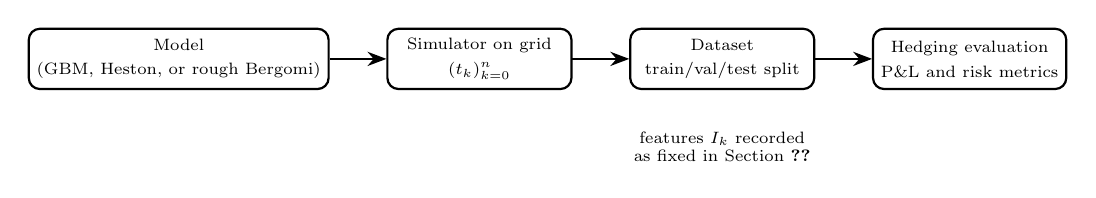
\begin{tikzpicture}[
    scale=0.85,
    every node/.style={transform shape},
    box/.style={draw, thick, rounded corners, minimum width=2.75cm, minimum height=0.9cm, align=center},
    arr/.style={-{Stealth[length=2.4mm]}, thick},
    node distance=0.85cm
]
\node[box] (model) {\scriptsize Model\\[-0.5mm]\scriptsize (GBM, Heston, or rough Bergomi)};
\node[box, right=of model] (sim) {\scriptsize Simulator on grid\\[-0.5mm]\scriptsize $(t_k)_{k=0}^n$};
\node[box, right=of sim] (data) {\scriptsize Dataset\\[-0.5mm]\scriptsize train/val/test split};
\node[box, right=of data] (hedge) {\scriptsize Hedging evaluation\\[-0.5mm]\scriptsize P\&L and risk metrics};

\draw[arr] (model) -- (sim);
\draw[arr] (sim) -- (data);
\draw[arr] (data) -- (hedge);

\node[below=5mm of data, font=\scriptsize, align=center]
{features $I_k$ recorded\\as fixed in Section~\ref{sec:hedging_frameworks}};
\end{tikzpicture}
\caption{Block diagram of the simulation pipeline: a model defines a simulator, which generates a dataset used for hedging evaluation under a fixed comparison protocol.}
\label{fig:sim_pipeline_block}
\end{figure}

\subsection{Time Discretisation and Monte Carlo Protocol}
\label{subsec:mc_protocol}

This subsection fixes the model-agnostic Monte Carlo interface used throughout the dissertation. 
As in \cite{Buehler2019DeepHedging}, we set up a single protocol that all methods use. This includes a shared discrete trading grid, a shared information set, and a shared rule for calculating trading gains, transaction costs, and final profit and loss.
Next, we explain how simulated scenarios are saved as datasets and divided into training, validation, and test sets. These sets will be used later for deep hedging and for reporting out-of-sample performance \cite{Buehler2019DeepHedging,Horvath2021DeepRough}.
We do not discuss model-specific simulation schemes here. These will be covered in the following subsections.

\begin{definition}[Trading grid and simulation grid]
\label{def:sim_grid}
Fix a maturity $T>0$ and an integer $n\ge 1$. 
The common \emph{trading grid} is
\[
0=t_0<t_1<\cdots<t_n=T.
\]
All strategies trade only at these times and hold positions $\delta_k$ on $[t_k,t_{k+1})$ as in Definition~\ref{def:comparison_grid}. 
In the simulation framework we use the same grid to discretise the model dynamics and to record the state variables needed to compute
\[
S_k:=S_{t_k},\qquad k=0,\dots,n,
\]
as well as any auxiliary factors required by the data-generating model.
\end{definition}

\begin{remark}[Why the simulation grid is fixed]
\label{rem:fixed_grid}
Using the same grid for all methods ensures that any performance differences stem from the hedging approach itself, not from different discretisations or trading opportunities.
The grid size $n$ is also used as a control variable in our experiments. In later chapters, we change $n$ to examine how discretisation affects results when there are transaction costs and rough volatility \cite{Buehler2019DeepHedging} and \cite{Horvath2021DeepRough}.
\end{remark}

\begin{definition}[Monte Carlo sample and scenario space]
\label{def:mc_sample}
Let $\mathsf{M}$ denote a chosen continuous-time model for the underlying (GBM or rough Bergomi). 
A \emph{scenario} is a simulated path of all model variables on the grid $(t_k)_{k=0}^n$, in particular the price path $(S_k)_{k=0}^n$. 
A Monte Carlo dataset of size $N$ is a collection of i.i.d.\ scenarios
\[
\mathcal{D}_N := \left\{\omega^{(i)}\right\}_{i=1}^N,
\]
generated under $\mathsf{M}$ with a fixed parameter set and a fixed random seed protocol, as in \cite{Buehler2019DeepHedging}.
\end{definition}

\begin{definition}[Recorded information and feature vectors]
\label{def:recorded_features}
For each scenario and each trading time $t_k$, we record the feature vector
\[
I_k := (t_k,\; S_k,\; \tau_k,\; \delta_{k-1}), \qquad \tau_k := T-t_k,
\]
as fixed by the comparison protocol in Definition~\ref{def:comparison_information}. 
No method is allowed to observe latent states of the data-generating model (such as the instantaneous variance in a stochastic-volatility model). 
All strategies are therefore functions of $I_k$ only, as in Section~\ref{sec:hedging_frameworks}.
\end{definition}

\begin{remark}[Fairness and data access]
\label{rem:data_access}
Delta hedging uses an assumed-model pricing engine to compute $\Delta^{\mathrm{assumed}}(t_k,S_k;\hat\theta)$ from the same observed inputs, while deep hedging uses $I_k$ as network inputs. 
Both methods are evaluated on identical scenarios $\omega^{(i)}$, identical costs, and identical constraints; see Section~\ref{sec:hedging_frameworks}. 
This is the standard experimental interface advocated in \cite{Buehler2019DeepHedging}.
\end{remark}

\begin{definition}[Train/validation/test split]
\label{def:split}
We partition $\mathcal{D}_N$ into three disjoint subsets:
\[
\mathcal{D}_N = \mathcal{D}_{\mathrm{train}} \,\dot\cup\, \mathcal{D}_{\mathrm{val}} \,\dot\cup\, \mathcal{D}_{\mathrm{test}}.
\]
The training set is used to minimise the empirical risk objective, the validation set is used for model selection and early stopping, and the test set is used only for out-of-sample reporting of hedging performance \cite{Buehler2019DeepHedging,Horvath2021DeepRough}.
\end{definition}

\begin{remark}[Reproducibility]
\label{rem:reproducibility}
To ensure reproducibility, random seeds are fixed for scenario generation and network initialisation, and the split defined in Definition~\ref{def:split} is maintained across all methods and hyperparameter variations.
This approach is essential for comparing tail-sensitive objectives such as expected shortfall and entropic risk \cite{FoellmerSchied2016} and implemented in \cite{Buehler2019DeepHedging}.
\end{remark}

\begin{definition}[Pathwise profit-and-loss evaluation]
\label{def:pathwise_pl_eval}
Fix a payoff $Z=g(S_T)$, initial capital $p_0$, and a strategy $\delta=(\delta_k)_{k=0}^{n-1}$. 
For a given scenario $\omega^{(i)}$, the \emph{pathwise terminal profit-and-loss} is computed by
\[
\mathrm{PL}_T^{(i)}(Z,p_0,\delta)
=
-\,Z^{(i)} + p_0 + \sum_{k=0}^{n-1}\delta_k^{(i)}\,(S_{k+1}^{(i)}-S_k^{(i)}) - C_T^{(i)}(\delta),
\]
with proportional costs as in Definition~\ref{def:comparison_costs_constraints}. 
Performance metrics (empirical distribution, VaR, expected shortfall, entropic risk) are then evaluated from the sample $\{\mathrm{PL}_T^{(i)}\}_{i\in\mathcal{D}_{\mathrm{test}}}$, in the spirit of \cite{Buehler2019DeepHedging}.
\end{definition}

\begin{algorithm}[H]
\caption{Scenario generation and dataset construction}
\label{alg:dataset_construction}
\begin{algorithmic}[1]
\Require Model $\mathsf{M}$ (GBM or rough Bergomi), parameters, grid $(t_k)_{k=0}^n$, dataset size $N$, cost coefficient $\lambda$, payoff function $g$
\Ensure Dataset $\mathcal{D}_N$ containing recorded paths and features $(S_k,I_k)_{k=0}^{n}$

\State Fix random seed(s) for reproducibility
\For{$i=1,\dots,N$}
    \State Simulate one scenario $\omega^{(i)}$ under $\mathsf{M}$ on $(t_k)_{k=0}^n$ and record $(S_k^{(i)})_{k=0}^n$
    \State Set $\delta_{-1}^{(i)}\gets 0$
    \For{$k=0,\dots,n-1$}
        \State Record features $I_k^{(i)}\gets(t_k,S_k^{(i)},T-t_k,\delta_{k-1}^{(i)})$
    \EndFor
    \State Record payoff $Z^{(i)}\gets g(S_n^{(i)})$
\EndFor
\State Split $\mathcal{D}_N$ into $\mathcal{D}_{\mathrm{train}},\mathcal{D}_{\mathrm{val}},\mathcal{D}_{\mathrm{test}}$ as in Definition~\ref{def:split}
\end{algorithmic}
\end{algorithm}

\begin{algorithm}[H]
\caption{Out-of-sample hedging evaluation on a fixed test set}
\label{alg:hedging_evaluation}
\begin{algorithmic}[1]
\Require Test scenarios $\mathcal{D}_{\mathrm{test}}$, strategy rule (delta engine or trained network), initial capital $p_0$, proportional cost coefficient $\lambda$
\Ensure Sample $\{\mathrm{PL}_T^{(i)}\}_{i\in\mathcal{D}_{\mathrm{test}}}$ and reported risk metrics

\For{each scenario $\omega^{(i)}\in\mathcal{D}_{\mathrm{test}}$}
    \State Initialise $\delta_{-1}^{(i)}\gets 0$ and set cumulative cost $C^{(i)}\gets 0$
    \For{$k=0,\dots,n-1$}
        \State Observe $I_k^{(i)}=(t_k,S_k^{(i)},T-t_k,\delta_{k-1}^{(i)})$
        \State Compute new position $\delta_k^{(i)}$ from the chosen strategy rule
        \State Update cost $C^{(i)}\gets C^{(i)}+\lambda S_k^{(i)}|\delta_k^{(i)}-\delta_{k-1}^{(i)}|$
    \EndFor
    \State Compute $\mathrm{PL}_T^{(i)}\gets -Z^{(i)}+p_0+\sum_{k=0}^{n-1}\delta_k^{(i)}(S_{k+1}^{(i)}-S_k^{(i)})-C^{(i)}$
\EndFor
\State Report empirical distribution of $\mathrm{PL}_T$ and tail-risk metrics (VaR/ES/entropic risk) on $\mathcal{D}_{\mathrm{test}}$
\end{algorithmic}
\end{algorithm}

\begin{remark}[What Section~\ref{subsec:mc_protocol} does and does not fix]
\label{rem:protocol_scope}
This subsection fixes the grid, the Monte Carlo interface, the recorded features, and the dataset split. 
It does not yet describe the exact dynamics of $\mathsf{M}$ or the numerical method used to create scenarios.
The next sections give these model-specific details for GBM (Section~\ref{subsec:gbm_sim}) and rough Bergomi (Section~\ref{subsec:rb_sim}), based on the simulation discussions in \cite{BayerFriz2016} and the deep-hedging work in \cite{Horvath2021DeepRough}.
\end{remark}
\newpage

\subsection{Simulating Markovian Benchmark Models}
\label{subsec:gbm_sim}

Two Markovian benchmark models are used throughout this dissertation.
Geometric Brownian motion (GBM) provides the canonical constant-volatility
reference, used both as the controlled benchmark of
Section~\ref{subsec:results_gbm} and as a transfer-learning source in
Section~\ref{sec:6_3_4}.
The Heston \cite{Heston1993} stochastic-volatility model provides a
stochastic-variance Markovian comparator, used as the analytical PDE delta
benchmark in Section~\ref{sec:6_3_1} and likewise as a transfer-learning
source in Section~\ref{sec:6_3_4}. Both models are Markovian (in $(S_t)$
and $(S_t, V_t)$ respectively), in contrast to the non-Markovian rough
Bergomi dynamics introduced in Section~\ref{subsec:rb_sim}.

\begin{definition}[Markovian benchmark dynamics]
\label{def:markovian_dynamics}
\label{def:gbm_discounted}
Under the discounted risk-neutral measure $\mathbb{Q}$:

\textbf{(a) Geometric Brownian motion (Black--Scholes).} The asset price
process satisfies
\begin{equation}\label{eq:gbm_sde}
  dS_t = \sigma\, S_t\, dW_t,
  \qquad S_0 > 0, \qquad \sigma > 0,
\end{equation}
where $W$ is a standard $\mathbb{Q}$-Brownian motion \cite{BlackScholes1973}.

\textbf{(b) Heston \cite{Heston1993} stochastic volatility.} The asset price
and variance jointly satisfy
\begin{align}
  dS_t &= \sqrt{V_t}\, S_t\, dW^S_t,
  \qquad S_0 > 0, \label{eq:heston_S}\\
  dV_t &= \kappa(\theta - V_t)\, dt + \sigma_v \sqrt{V_t}\, dW^V_t,
  \qquad V_0 > 0, \label{eq:heston_V}\\
  d\langle W^S, W^V\rangle_t &= \rho\, dt, \label{eq:heston_corr}
\end{align}
where $\kappa > 0$ is the variance mean-reversion speed, $\theta > 0$ is the
long-run mean variance, $\sigma_v > 0$ is the vol-of-vol, and
$\rho \in [-1, 1]$ is the leverage correlation.
\end{definition}

\begin{proposition}[Discrete-time discretisation]
\label{prop:markovian_disc}
\label{prop:gbm_exact_transition}
Let $(t_k)_{k=0}^n$ be the uniform grid from Definition~\ref{def:sim_grid}
with step $\Delta t := T/n$.

\textbf{(a) GBM exact grid transition.} Under
Definition~\ref{def:markovian_dynamics}(a), the exact one-step transition is
\begin{equation}\label{eq:gbm_disc}
  S_{t_{k+1}} = S_{t_k} \exp\!\left(-\tfrac{1}{2}\sigma^2 \Delta t
  + \sigma \sqrt{\Delta t}\, Z_k\right),
  \qquad k = 0, \ldots, n-1,
\end{equation}
where $(Z_k)_{k=0}^{n-1}$ are i.i.d.\ standard normal random variables.
This discretisation is exact in distribution at grid points; conditional on
$\mathcal{F}_{t_k}$, $S_{t_{k+1}}$ is lognormal.

\textbf{(b) Heston full-truncation Euler.} Under
Definition~\ref{def:markovian_dynamics}(b), the full-truncation Euler scheme
\cite{LordKoekkoekVanDijk2010} is
\begin{align}
  V_{t_{k+1}} &= \max\!\Big( V_{t_k}
  + \kappa(\theta - V_{t_k}^+)\Delta t
  + \sigma_v \sqrt{V_{t_k}^+ \Delta t}\, Z^V_k,\; 0 \Big),
  \label{eq:heston_disc_V}\\
  S_{t_{k+1}} &= S_{t_k} \exp\!\left(-\tfrac{1}{2}V_{t_k}^+ \Delta t
  + \sqrt{V_{t_k}^+}\, dB_k\right), \label{eq:heston_disc_S}
\end{align}
where $V_t^+ := \max(V_t, 0)$, the correlated price increment is
$dB_k := \sqrt{\Delta t}\,(\rho\, Z^V_k + \sqrt{1-\rho^2}\, Z^S_k)$, and
$(Z^V_k, Z^S_k)$ are independent standard normals. This scheme is first-order
weakly convergent.
\end{proposition}

\begin{proof}
For part (a), apply It\^o's formula to $f(x)=\log x$ and integrate over
$[t_k,t_{k+1}]$. Starting from $dS_t=\sigma S_t\,dW_t$, the quadratic variation
is $d\langle S\rangle_t=\sigma^2 S_t^2\,dt$, giving
$d(\log S_t)=\sigma\,dW_t-\tfrac12\sigma^2\,dt$. Integration yields
$\log S_{t_{k+1}}-\log S_{t_k}=\sigma(W_{t_{k+1}}-W_{t_k})-\tfrac12\sigma^2\Delta t$.
Since $W_{t_{k+1}}-W_{t_k}\sim\mathcal N(0,\Delta t)$, writing
$W_{t_{k+1}}-W_{t_k}=\sqrt{\Delta t}\,Z_k$ with $Z_k\sim\mathcal N(0,1)$ and
exponentiating gives \eqref{eq:gbm_disc}; conditional lognormality is
immediate \cite{BlackScholes1973}.
For part (b), the full-truncation Euler scheme is the standard discretisation
of \eqref{eq:heston_S}--\eqref{eq:heston_corr} obtained by replacing the drift
and diffusion coefficients with their values at the previous grid point under
the truncation $V\mapsto V^+:=\max(V,0)$, and clamping the variance update at
zero. First-order weak convergence is established in
\cite{LordKoekkoekVanDijk2010}.
\end{proof}

\begin{remark}[Feller condition and discretisation contrast]
\label{rem:feller}
The Heston variance process $V_t$ remains strictly positive almost surely
if and only if $2\kappa\theta \geq \sigma_v^2$ (the Feller condition).
Calibrations may violate this condition: the calibrated Heston parameters
used in Section~\ref{sec:6_3_1} have slack
$2\kappa\theta - \sigma_v^2 \approx -0.20$, meaning $V_t$ may touch zero with
positive probability. The full-truncation scheme of
Proposition~\ref{prop:markovian_disc}(b) remains numerically well-defined in
this regime through the explicit $\max(V_t, 0)$ clamping. No analogous
condition is required for GBM, where $V_t = \sigma^2$ is deterministic. The
GBM discretisation of Proposition~\ref{prop:markovian_disc}(a) is exact at
grid points; the Heston discretisation of
Proposition~\ref{prop:markovian_disc}(b) is first-order weakly convergent.
\end{remark}

\begin{algorithm}[H]
\caption{Path simulation for Markovian benchmark models}\label{alg:markovian_sim}
\begin{algorithmic}[1]
\Require Initial spot $S_0$; time horizon $T$; time steps $n$;
sample size $N$; random seed $\omega$.

\State \textbf{(a) GBM.} \emph{Inputs: volatility $\sigma$.}
\State Initialise RNG with seed $\omega$.
\State Sample $\mathbf{Z} \in \mathbb{R}^{N \times n}$ with i.i.d.\ $\mathcal{N}(0,1)$ entries.
\State $\Delta t \leftarrow T / n$.
\State $\mathbf{L} \leftarrow -\tfrac{1}{2}\sigma^2 \Delta t + \sigma \sqrt{\Delta t}\, \mathbf{Z}$.
\State $\mathbf{C} \leftarrow$ row-wise cumulative sum of $\mathbf{L}$, prepended with a column of zeros.
\State \Return $\mathbf{S} \leftarrow S_0 \exp(\mathbf{C})$ of shape $N \times (n+1)$.

\Statex
\State \textbf{(b) Heston.} \emph{Inputs: $V_0, \kappa, \theta, \sigma_v, \rho$.}
\State Initialise RNG with seed $\omega$; set $\rho_\perp \leftarrow \sqrt{1 - \rho^2}$.
\State Sample $\mathbf{Z}^V, \mathbf{Z}^S \in \mathbb{R}^{N \times n}$ with i.i.d.\ $\mathcal{N}(0,1)$ entries.
\State Initialise $\mathbf{V}[:, 0] \leftarrow V_0$; $\Delta t \leftarrow T/n$.
\For{$k = 0, \ldots, n-1$}
  \State $\mathbf{V}^+_k \leftarrow \max(\mathbf{V}[:,k], 0)$.
  \State $\mathbf{V}[:, k+1] \leftarrow \max\!\Big(\mathbf{V}[:,k] + \kappa(\theta - \mathbf{V}^+_k)\Delta t
  + \sigma_v \sqrt{\mathbf{V}^+_k \Delta t}\, \mathbf{Z}^V[:,k],\; 0\Big)$.
  \State $\mathbf{dB}_k \leftarrow \sqrt{\Delta t}\,\big(\rho\, \mathbf{Z}^V[:,k] + \rho_\perp\, \mathbf{Z}^S[:,k]\big)$.
  \State $\mathbf{L}[:, k] \leftarrow -\tfrac{1}{2}\mathbf{V}^+_k \Delta t + \sqrt{\mathbf{V}^+_k}\, \mathbf{dB}_k$.
\EndFor
\State $\mathbf{C} \leftarrow$ row-wise cumulative sum of $\mathbf{L}$, prepended with a column of zeros.
\State \Return $\mathbf{S} \leftarrow S_0 \exp(\mathbf{C})$, $\mathbf{V}$ both of shape $N \times (n+1)$.
\end{algorithmic}
\end{algorithm}

Both \texttt{GBM.simulate(seed=...)} and \texttt{Heston.simulate(seed=...)} are
implemented as PyTorch \texttt{nn.Module} instances with explicit seeded RNG,
fully autograd-compatible to support the gradient-based experiments of
Section~\ref{sec:6_3_5}. Path generation is byte-deterministic given
the seed argument; the seeding protocol of Appendix~\ref{app:reproducibility}
governs caller-side state for reproducibility. The GBM implementation lives in
\path{src/world_gbm.py} (used by the benchmark of
Section~\ref{subsec:results_gbm}) and \path{deep_hedging/core/gbm.py}
(used by the transfer-learning experiments of Section~\ref{sec:6_3_4}); the
Heston implementation lives in \path{deep_hedging/core/heston.py}.

\begin{figure}[H]
  \centering
  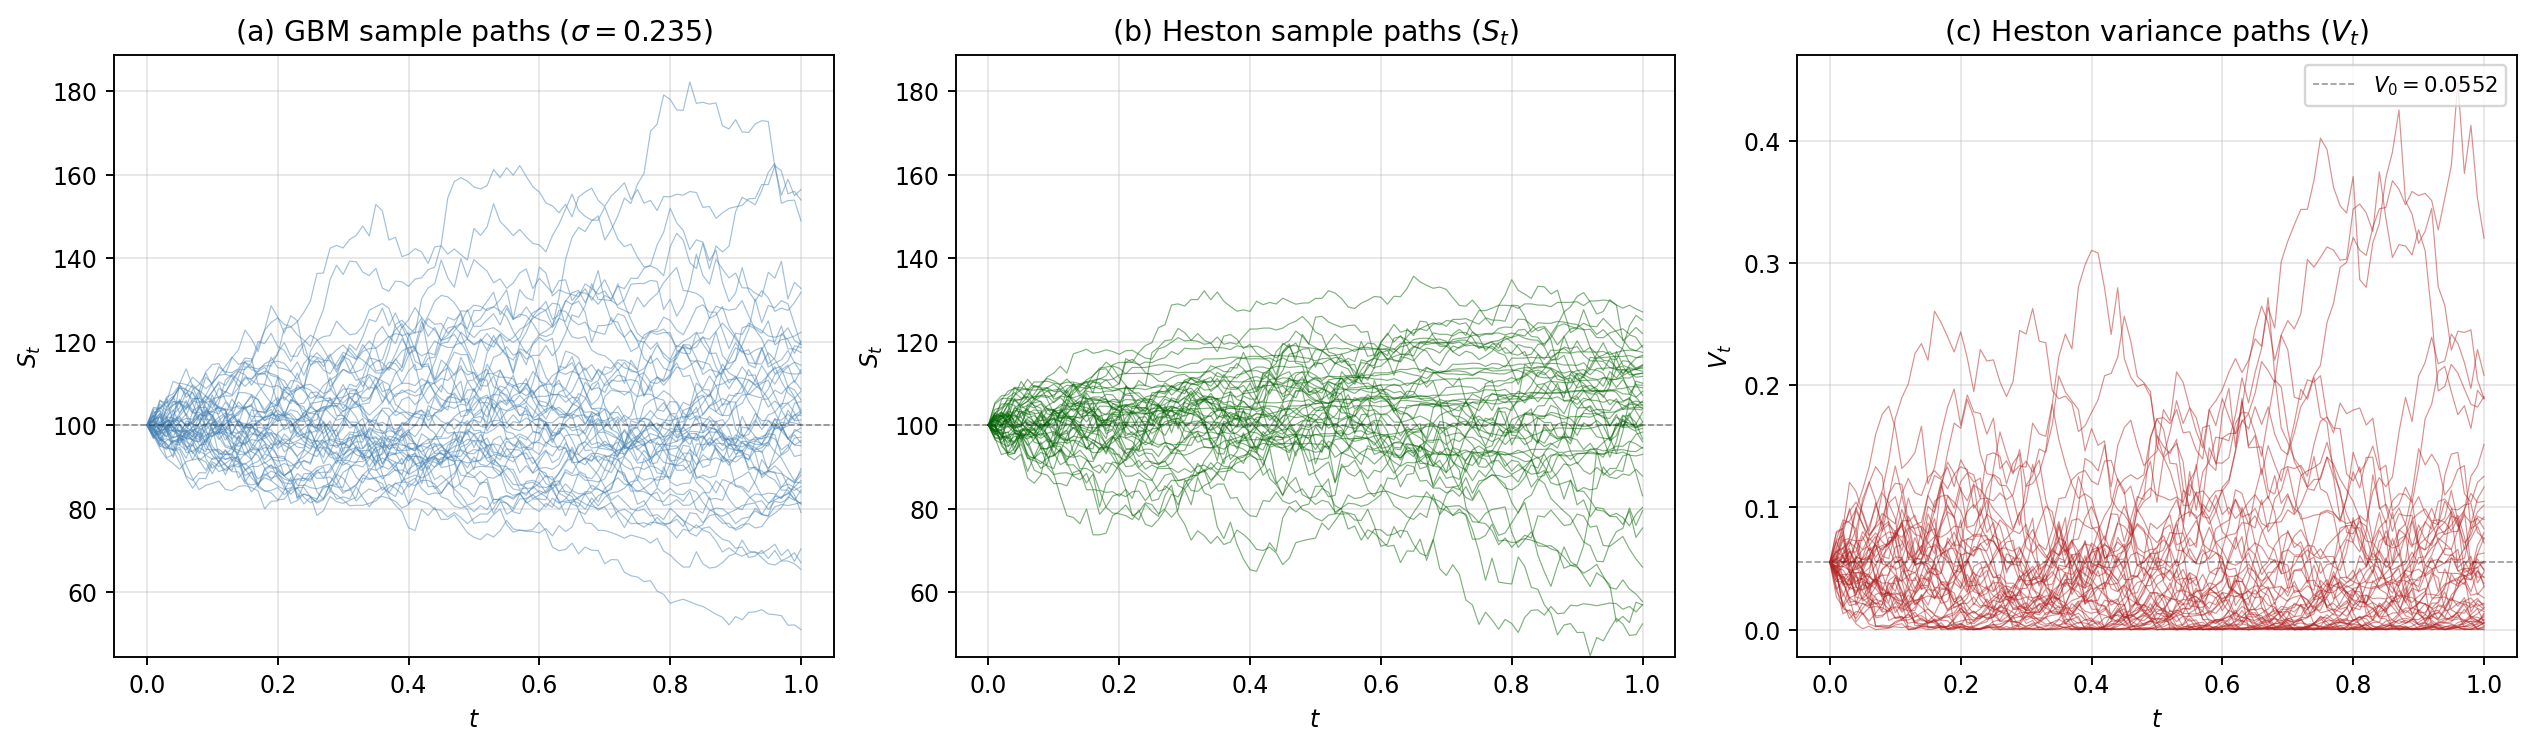
\includegraphics[width=\textwidth]{figures/5_2_markovian_paths.png}
  \caption{Sample paths from the two Markovian benchmark models.
    \textbf{(a)} 50 GBM sample paths at $\sigma = 0.235$.
    \textbf{(b)} 50 Heston sample paths $(S_t)$ at calibrated parameters
    $\kappa = 1.0$, $\theta = V_0 = 0.235^2$, $\sigma_v = 0.554$, $\rho = -0.7$
    (calibration documented in Section~\ref{sec:6_3_1}).
    \textbf{(c)} 50 Heston variance paths $(V_t)$ at the same calibration.
    All trajectories use the same path seed and time grid
    ($S_0 = 100$, $T = 1$, $n = 100$).}
  \label{fig:markovian_paths}
\end{figure}
\FloatBarrier

\subsection{Simulating Rough Bergomi}
\label{subsec:rb_sim}

The rough Bergomi model serves as the primary data-generating process for the numerical experiments.
While Chapter~\ref{sec:rough_volatility} presents the modelling motivation and theoretical foundations, the practical challenge is to generate sample paths efficiently on a discrete grid. The differentiable rough Bergomi simulator used in this dissertation is implemented in the accompanying Python package \texttt{deep\_hedging}, released at \url{https://github.com/westgluf/thesis_code}. The hybrid Volterra/fBm driver is implemented in \path{deep_hedging/core/volterra.py}, and the rough Bergomi model wrapper in \path{deep_hedging/core/rough_bergomi.py}. Complete reproducibility information is documented in Appendix~\ref{app:reproducibility}. This includes random seeds, the dataset generation protocol, hyperparameters, and the frozen master test set used throughout Section~\ref{sec:numerical_experiments}.

\begin{definition}[Discrete-time rough Bergomi simulator interface]
\label{def:rb_sim_interface}
Fix a trading/simulation grid $(t_k)_{k=0}^n$ as in Definition~\ref{def:sim_grid}, an initial price $S_0>0$, a Hurst parameter $H\in(0,\tfrac12)$, volatility-of-volatility $\eta>0$, correlation $\rho\in[-1,1]$, and a forward variance curve $\xi_0:[0,T]\to(0,\infty)$.
Given a number of Monte Carlo paths $N\in\mathbb{N}$, the rough Bergomi simulator returns at least the price array
\[
\bigl\{S^{(i)}_{t_k}\bigr\}_{i=1,\dots,N;\,k=0,\dots,n}.
\]
Optionally, for diagnostics and validation it may also return the variance array $\{v^{(i)}_{t_k}\}$ and the Volterra driver array $\{(W^{H})^{(i)}_{t_k}\}$ on the same grid.
\end{definition}

\begin{remark}[Why the Volterra/fBm driver is the key numerical bottleneck]
\label{rem:rb_driver_bottleneck}
In rough-volatility models, most of the computational cost comes from generating the rough Gaussian driver on the grid, rather than from updating the price.
The Volterra or fractional Brownian motion (fBm) approach captures long-range dependence and produces highly correlated Gaussian vectors. Because of this, simple sampling methods are costly and require specialised techniques \cite{BayerFriz2016} and shown by data in \cite{GatheralRough}.
\end{remark}

\begin{definition}[Volterra driver on a grid]
\label{def:rb_volterra_grid}
Let $(\Delta W_j)_{j=0}^{n-1}$ be Brownian increments on the grid, with $\Delta W_j:=W_{t_{j+1}}-W_{t_j}$.
A generic discrete Volterra approximation of the rough driver takes the form
\[
W^H_{t_k}\approx \sum_{j=0}^{k-1} K_{k,j}\,\Delta W_j,
\qquad k=1,\dots,n,
\]
for weights $K_{k,j}$ determined by the kernel $(t-s)^{H-\frac12}$ and the chosen discretisation, as described in \cite{BayerFriz2016}.
In the project codebase, this step is implemented via a hybrid approximation that treats the near-diagonal singular regime accurately and approximates the long-memory tail more coarsely; see \path{deep_hedging/core/volterra.py}.
\end{definition}

\begin{remark}[Why we do not use Cholesky as the baseline simulator]
\label{rem:rb_no_cholesky}
One direct method involves constructing the dense covariance matrix of the discretised driver and sample via Cholesky factorisation, as detailed in Section~4 of \cite{BayerFriz2016}.
This is conceptually simple but becomes very slow at fine time grids due to dense linear algebra, and \cite{BayerFriz2016} explicitly highlights faster structure-exploiting schemes as an important direction.
The project codebase provides a Cholesky-based reference implementation in \path{deep_hedging/core/volterra_exact.py}. However, the hybrid scheme is adopted as the primary practical simulator; the Cholesky implementation is used only for the validation comparison of Section~\ref{subsec:sim_validation}.
\end{remark}

\begin{definition}[Rough variance and correlated price innovations on the grid]
\label{def:rb_variance_price_grid}
Let $(W^H_{t_k})_{k=0}^n$ be a discretised Volterra driver as in Definition~\ref{def:rb_volterra_grid}.
The rough Bergomi variance on the grid is defined by
\[
v_{t_k}
=
\xi_0(t_k)\exp\!\left(\eta W^H_{t_k}-\frac12\eta^2 t_k^{2H}\right),
\qquad k=0,\dots,n,
\]
\cite{BayerFriz2016}.
To simulate the discounted price on the grid, we use a log-Euler update
\[
S_{t_{k+1}}
=
S_{t_k}\exp\!\left(-\frac12 v_{t_k}\Delta t_k+\sqrt{v_{t_k}\Delta t_k}\,Z_k^{(B)}\right),
\qquad k=0,\dots,n-1,
\]
where $(Z_k^{(B)})$ are standard normal innovations correlated with the volatility driver noise at correlation level $\rho$, following the rough Bergomi construction in \cite{BayerFriz2016}.
\end{definition}

\begin{algorithm}[H]
\caption{Simulating one rough Bergomi path on a grid (hybrid driver)}
\label{alg:rb_single_path}
\begin{algorithmic}[1]
\Require $S_0$, grid $(t_k)_{k=0}^n$, parameters $(H,\eta,\rho)$, forward variance curve $\xi_0(\cdot)$
\Ensure One simulated path $(S_{t_k})_{k=0}^n$ and optionally $(v_{t_k})_{k=0}^n$, $(W^H_{t_k})_{k=0}^n$
\State Generate a discretised Volterra driver $(W^H_{t_k})_{k=0}^n$ on $(t_k)$ using a hybrid scheme as in Definition~\ref{def:rb_volterra_grid}
\State Compute variance on the grid via $v_{t_k}=\xi_0(t_k)\exp(\eta W^H_{t_k}-\tfrac12\eta^2 t_k^{2H})$ for $k=0,\dots,n$
\State Generate i.i.d.\ standard normals $(Z_k^{(1)},Z_k^{(2)})_{k=0}^{n-1}$ and set $Z_k^{(B)}:=\rho Z_k^{(1)}+\sqrt{1-\rho^2}\,Z_k^{(2)}$
\State Set $S_{t_0}\gets S_0$
\For{$k=0,\dots,n-1$}
    \State Update $S_{t_{k+1}}\gets S_{t_k}\exp(-\tfrac12 v_{t_k}\Delta t_k+\sqrt{v_{t_k}\Delta t_k}\,Z_k^{(B)})$
\EndFor
\Statex \textbf{Implementation hook:} Step 1 is implemented in \path{deep_hedging/core/volterra.py} and the model wrapper in \path{deep_hedging/core/rough_bergomi.py}.
\end{algorithmic}
\end{algorithm}

\begin{algorithm}[H]
\caption{Vectorised rough Bergomi dataset generation (paths only)}
\label{alg:rb_dataset_generation}
\begin{algorithmic}[1]
\Require Grid $(t_k)_{k=0}^n$, parameters $(H,\eta,\rho)$, $\xi_0(\cdot)$, number of paths $N$
\Ensure Path dataset $\{(S^{(i)}_{t_k})_{k=0}^n\}_{i=1}^N$ (to be wrapped into $\mathcal{D}_N$ and split as in Definition~\ref{def:split})
\State Fix random seed(s) for reproducibility
\For{$i=1,\dots,N$}
    \State Simulate one rough Bergomi path $(S^{(i)}_{t_k})_{k=0}^n$ using Algorithm~\ref{alg:rb_single_path}
\EndFor
\State Store all paths as a Monte Carlo dataset and apply the split protocol from Definition~\ref{def:split}
\end{algorithmic}
\end{algorithm}

\begin{figure}[H]
\centering
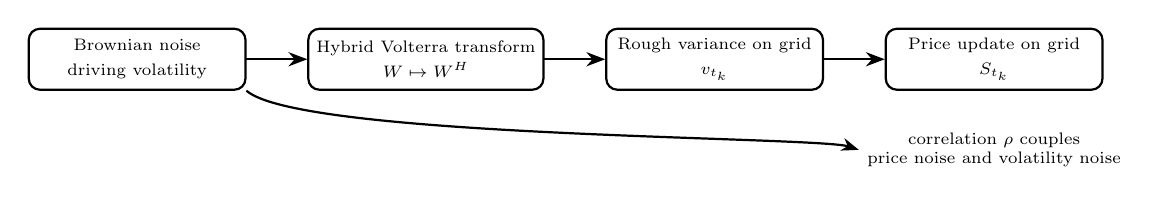
\begin{tikzpicture}[
    scale=0.86,
    every node/.style={transform shape},
    box/.style={draw, thick, rounded corners, minimum width=3.2cm, minimum height=0.9cm, align=center},
    arr/.style={-{Stealth[length=2.4mm]}, thick},
    node distance=0.9cm
]
\node[box] (W) {\scriptsize Brownian noise\\[-0.5mm]\scriptsize driving volatility};
\node[box, right=of W] (WH) {\scriptsize Hybrid Volterra transform\\[-0.5mm]\scriptsize $W\mapsto W^H$};
\node[box, right=of WH] (v) {\scriptsize Rough variance on grid\\[-0.5mm]\scriptsize $v_{t_k}$};
\node[box, right=of v] (S) {\scriptsize Price update on grid\\[-0.5mm]\scriptsize $S_{t_k}$};

\draw[arr] (W) -- (WH);
\draw[arr] (WH) -- (v);
\draw[arr] (v) -- (S);

\node[below=5mm of S, font=\scriptsize, align=center] (corr)
{correlation $\rho$ couples\\price noise and volatility noise};
\draw[-{Stealth[length=2.2mm]}, thick] (W.south east) .. controls +(0.8,-0.7) and +(-0.6,0.2) .. (corr.west);

\end{tikzpicture}
\caption{Rough Bergomi simulation pipeline on a grid: Brownian noise is mapped to a rough Volterra driver, which generates rough variance and then drives the log-Euler price update \cite{BayerFriz2016}.}
\label{fig:rb_pipeline}
\end{figure}
\FloatBarrier

\begin{remark}[Computational cost and the accuracy--speed trade-off]
\label{rem:rb_cost_tradeoff}
Hybrid schemes aim to preserve accuracy near the kernel singularity while reducing the cost of long-memory aggregation \cite{BayerFriz2016}.
This matters directly for deep hedging, since training requires repeated evaluation of objectives over large Monte Carlo samples and many optimisation iterations \cite{Buehler2019DeepHedging} and \cite{Horvath2021DeepRough}.
By fixing a single simulator in this subsection, we ensure that the dataset protocol from Section~\ref{subsec:mc_protocol} can be executed at the scale required for robust tail-risk comparisons.
\end{remark}

A comprehensive numerical validation of this simulator, including a
convergence study and an exact-Cholesky benchmark, is presented in
Section~\ref{subsec:sim_validation}.

The simulator fixed in this subsection is used to generate all rough-volatility datasets in Sections~\ref{sec:numerical_experiments}--\ref{sec:discussion}.
With rough Bergomi paths available under the common dataset protocol from Section~\ref{subsec:mc_protocol}, Section~\ref{sec:numerical_experiments} compares delta hedging and deep hedging under identical trading rules and identical data access.

\subsection{Numerical Validation of Simulators}
\label{subsec:sim_validation}

Before deploying the three simulators of Sections~\ref{subsec:gbm_sim} and
\ref{subsec:rb_sim} in the hedging experiments of
Section~\ref{subsec:results_rough_vol}, we subject them to numerical
validation. The Markovian benchmarks (GBM, Heston) inherit a long literature
of discretisation error analysis and are validated through reproducibility
checks; the rough Bergomi simulator, which uses the hybrid Volterra scheme of
\cite{BennedsenLundePakkanen2017}, is subjected to three independent
numerical validations described below.

\paragraph{GBM benchmark reproducibility.}
The Section~\ref{subsec:results_gbm} GBM benchmark pipeline was independently
re-executed in the current Python environment and reproduces byte-identically
against the canonical archived output across the full evaluation cell
(50\,000 test paths at $\bar{\sigma} = 0.20$, $\lambda = 0$, seed $0$,
deep-hedger oracle regime), including all six summary metrics, the
100\,000 test-set P\&L arrays, the trained neural-network weights, and the
feature-normalisation statistics. Results of this verification are archived
under \path{results/gbm_recheck/} in the codebase.

\paragraph{Convergence study.}
We measure the discretisation error of $\mathrm{ES}_{0.95}$ as a function of
grid resolution $n \in \{50, 100, 200, 400, 800, 1600\}$, holding all other
parameters fixed at the canonical calibration ($H = 0.07$, $\eta = 1.9$,
$\rho = -0.7$, $\xi_0 = 0.235^2$). A log-log linear fit yields empirical
slope $\hat{\alpha} \approx 0.913$ ($95\,\%$ CI $[0.722, 1.104]$). The
asymptotic rate for the hybrid scheme of \cite{BennedsenLundePakkanen2017}
at $H = 0.07$ is $\alpha = H + 1/2 \approx 0.57$. The empirical rate exceeds
the asymptotic rate in the finite-$n$ regime tested, consistent with the
hybrid scheme's faster-than-asymptotic convergence at moderate grids
(Figure~\ref{fig:convergence_alpha}). Richardson extrapolation gives
$\mathrm{ES}_{0.95}^{\infty} \approx 8.82$, with relative error at $n = 100$
of approximately $28.7\,\%$.

\begin{figure}[H]
  \centering
  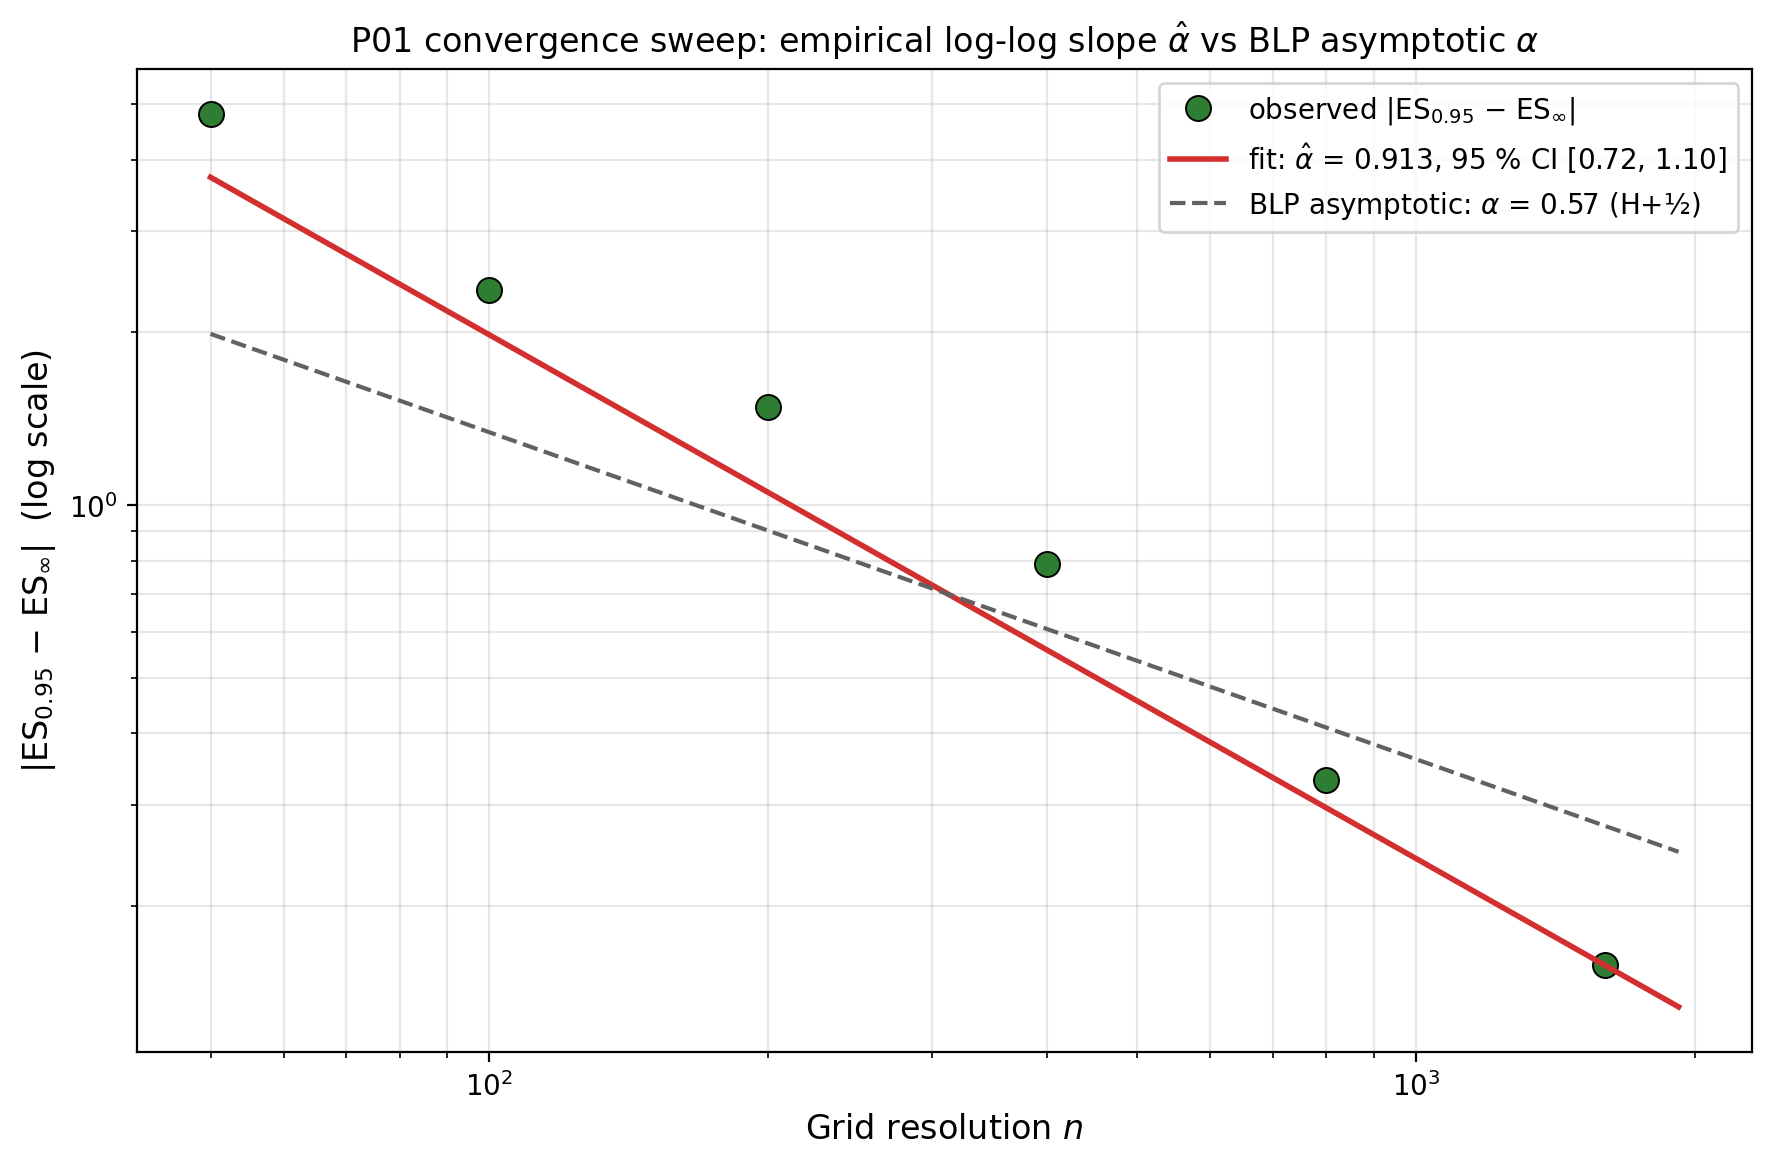
\includegraphics[width=0.85\textwidth]{figures/5_4_convergence_alpha.png}
  \caption{Convergence of the hybrid rough Bergomi simulator at the
    canonical calibration. Log-log plot of $|\mathrm{ES}_{0.95}(n) -
    \mathrm{ES}_{0.95}^{\infty}|$ versus grid resolution $n$.
    Fitted slope $\hat{\alpha} \approx 0.913$ exceeds the
    \cite{BennedsenLundePakkanen2017} asymptotic rate
    $\alpha = H + 1/2 \approx 0.57$ in the regime tested. Shaded band
    shows the $95\,\%$ confidence interval of the fit.}
  \label{fig:convergence_alpha}
\end{figure}

\paragraph{Exact-Cholesky benchmark.}
At $N = 500\,000$ paths, the hybrid simulator output is compared against a
direct Cholesky-factorisation reference at the canonical calibration. The
Cholesky simulator computes the full covariance matrix of the fractional
Brownian motion and samples directly via Gaussian factorisation; it is
computationally prohibitive for training but provides an exact reference
for validation. Five validation criteria all pass: (i) marginal mean and
variance match within Monte Carlo noise; (ii) path-wise variance gap below
$2.2\,\%$; (iii) Kolmogorov--Smirnov test on terminal $W^H_T$ gives
$p = 0.926$; (iv) Gaussian moments (skewness, kurtosis) align; (v) lag-1
correlation structure matches. The terminal-distribution comparison is
illustrated in Figure~\ref{fig:cholesky_ks}.

\begin{figure}[H]
  \centering
  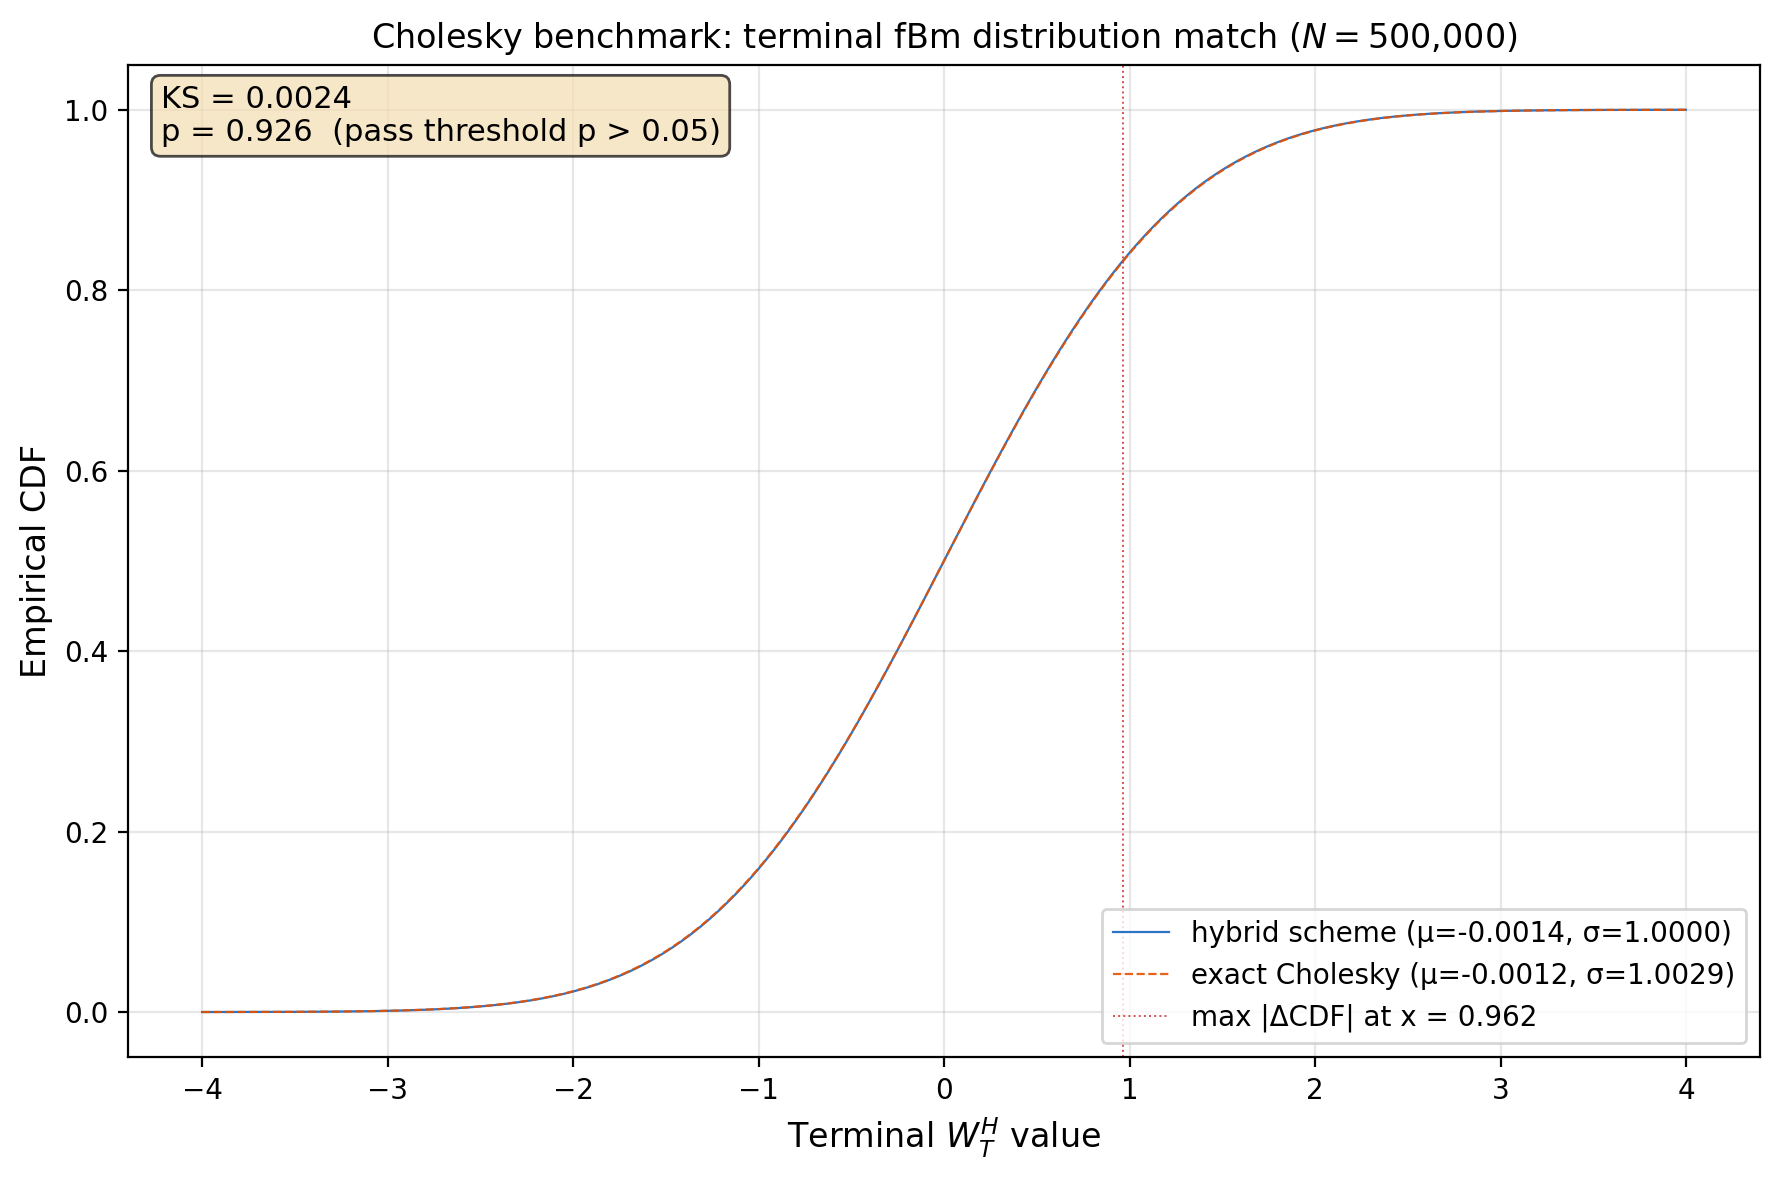
\includegraphics[width=0.85\textwidth]{figures/5_4_cholesky_ks.png}
  \caption{Exact-Cholesky benchmark at $N = 500\,000$. Empirical CDFs of
    the terminal fractional Brownian motion $W^H_T$ under the hybrid scheme
    (solid blue) and the exact Cholesky reference (dashed orange).
    Kolmogorov--Smirnov statistic location indicated; the high $p$-value
    ($p = 0.926$) and visually near-coincident CDFs confirm that the two
    distributions cannot be statistically distinguished.}
  \label{fig:cholesky_ks}
\end{figure}

The two validation protocols use the fixed seeding convention of
Appendix~\ref{app:reproducibility} and produce byte-identical outputs
across fresh Python subprocesses.

\section{Numerical Experiments and Sensitivity Analysis}
\label{sec:numerical_experiments}

\subsection{Setup}
\label{sec:numerical_setup}

This chapter presents the empirical analysis of the three hedging
strategies of Chapter~\ref{sec:hedging_frameworks} under two
data-generating models. Section~\ref{subsec:results_gbm} reports a
controlled Black--Scholes benchmark in which the analytical hedge is
known. Section~\ref{subsec:results_rough_vol} reports the rough Bergomi
target setting in which the four hypotheses of
Section~\ref{subsec:section4_hypotheses} are tested. The Black--Scholes
benchmark serves as a controlled validation of the deep hedging
implementation. The rough Bergomi setting then tests the same hypotheses
in a non-Markovian, mis-specified regime where all three strategies are
simultaneously misspecified.

Three hedging strategies are compared throughout. The Black--Scholes
delta of Section~\ref{subsubsec:bs_delta} observes only the spot price
$S_t$ and uses the constant volatility input $\sigma = \sqrt{\xi_0}$.
The true Heston PDE delta of Section~\ref{subsubsec:heston_delta}
observes both the spot $S_t$ and the instantaneous variance $V_t$. It
is computed by numerical solution of the two-dimensional Heston pricing
PDE under parameters calibrated to the rough Bergomi process. The
calibration procedure is documented in Section~\ref{sec:6_3_1}. The
deep hedger of Section~\ref{subsec:deep_hedging_framework} is a
flat-feature feedforward network observing only the spot $S_t$ and
trained to minimise the $\mathrm{ES}_{0.95}$ objective on simulated
paths.

The hedging metrics reported throughout this chapter are computed from
the terminal profit-and-loss distribution of
Definition~\ref{def:terminal_PL}. We report the expected shortfall at
confidence levels $\alpha = 0.95$ and $\alpha = 0.99$, the standard
deviation of $\mathrm{P\&L}$, the mean $\mathrm{P\&L}$, and the
mean per-strategy turnover (the average sum of absolute position
changes across the rebalancing grid). Headline numbers are reported as
a five-seed mean plus or minus one standard deviation unless stated
otherwise. Each evaluation uses 50{,}000 test paths.

The numerical experiments of Section~\ref{subsec:results_rough_vol}
share a common setup. The frozen master test set consists of 50{,}000
paths simulated under the canonical rough Bergomi calibration of
Section~\ref{subsec:rb_sim} with seed 2024. Each deep hedger is trained
from scratch on 80{,}000 simulated paths, with 20{,}000 paths held out
for validation and the master 50{,}000 paths reserved for out-of-sample
evaluation. All deep hedgers share the architecture
\texttt{DeepHedgerFNN(input\_dim=4, hidden\_dim=128, n\_res\_blocks=2)}
and the same training protocol (Adam optimiser, learning rate
$10^{-3}$, batch size 2048, 200 epochs, early-stopping patience 30).
The full reproducibility protocol, including all random seeds, dataset
generation, hyperparameters, and the master test set itself, is
documented in Appendix~\ref{app:reproducibility}.

The four hypotheses of Section~\ref{subsec:section4_hypotheses} are
tested across the rough Bergomi subsections as follows.
\begin{description}
  \item[H1] (heavier left tails for diffusion-based deltas):
        Section~\ref{sec:6_3_1}.
  \item[H4] (flat-feature sufficiency):
        Section~\ref{sec:6_3_3}.
  \item[H3] (uniform advantage under parameter perturbation):
        Sections~\ref{sec:6_3_4} and~\ref{sec:6_3_5}.
  \item[H2] (transaction costs reverse the rebalancing benefit):
        Section~\ref{sec:6_3_5}.
\end{description}
Section~\ref{sec:6_3_2} additionally reports a methodological
finding on the role of the risk objective.

\subsection{Results Under GBM (Benchmark)}
\label{subsec:results_gbm}

The Black--Scholes benchmark is a controlled validation of the
deep hedging implementation against an analytical reference. In the
frictionless GBM setting with the assumed-volatility input matched
to the data-generating volatility ($\bar\sigma = \sigma_{\mathrm{true}}$),
the Black--Scholes delta is the analytical replicating strategy and
realises zero $\mathrm{P\&L}$ in continuous time. Under discrete
rebalancing the BS delta becomes a strong but non-zero benchmark, and
we expect the deep hedger to match it in this regime. Across the full
benchmark grid we vary the assumed-volatility input
$\bar\sigma \in \{0.10, 0.15, 0.20, 0.25, 0.30\}$ and the proportional
cost coefficient $\lambda \in \{0,\, 10^{-4},\, 5{\cdot}10^{-4},\,
10^{-3}\}$. The data-generating volatility is fixed at
$\sigma_{\mathrm{true}} = 0.20$. Each cell is evaluated on $50{,}000$
test paths over ten independent training seeds. Two training regimes
are compared, the oracle hedger that trains at a single
$\bar\sigma = \sigma_{\mathrm{true}} = 0.20$ and the robust hedger that
trains over the family $\bar\sigma \in \{0.15, 0.20, 0.25\}$. The
benchmark pipeline is implemented in \path{src/world_gbm.py} and the
runs are archived under \path{results/gbm_deephedge/benchmark_6_2/}.

The correctly-specified cell ($\bar\sigma = 0.20$, $\lambda = 0$)
validates the implementation. The Black--Scholes delta achieves
$\mathrm{ES}_{0.95} = 0.0225 \pm 0.0000$ and the oracle deep hedger
achieves $\mathrm{ES}_{0.95} = 0.0213 \pm 0.0001$
(Table~\ref{tab:gbm_table2_oracle}). The deep hedger's small
absolute improvement of $0.0013$ in $\mathrm{ES}_{0.95}$ is statistically
significant at the per-seed level ($t = -12.63$, $p = 5{\cdot}10^{-7}$
on $n = 10$ paired seeds; Table~\ref{tab:gbm_table3_paired}) and
reflects the tail-aware $\mathrm{ES}_{0.95}$ training objective
relative to the pointwise replication target of the analytical delta.
The two strategies agree to within $6\%$ of the analytical value, as
expected when the assumed model is correctly specified.

Outside the correctly-specified cell the picture changes. When
$\bar\sigma$ underestimates the true volatility ($\bar\sigma = 0.10$),
the Black--Scholes delta degrades sharply to $\mathrm{ES}_{0.95} = 0.0550$
while the oracle deep hedger remains at $0.0213$ (the oracle DH does
not depend on $\bar\sigma$). The paired difference is $\Delta = -0.0338$
($t = -245.88$, $p \approx 10^{-18}$). At $\bar\sigma = 0.30$ the BS
delta degrades to $\mathrm{ES}_{0.95} = 0.0274$, again with a strongly
significant deep-hedger advantage of $\Delta = -0.0062$. The single
exception is $\bar\sigma = 0.25$, where the BS delta achieves
$\mathrm{ES}_{0.95} = 0.0205$ and slightly out-performs the oracle deep
hedger by $\Delta = +0.0008$ ($t = +8.75$, $p = 10^{-5}$). The slight
over-estimate of volatility produces a more conservative analytical
hedge that happens to dominate the tail-aware learned hedge in this
regime.

The cost grid reveals the second qualitative feature. As $\lambda$ grows
from $0$ to $10^{-3}$, both strategies degrade, but the relative
order is preserved (Table~\ref{tab:gbm_table2_oracle}). At
$\bar\sigma = 0.20$, the oracle deep hedger degrades from $0.0213$ at
$\lambda = 0$ to $0.0248$ at $\lambda = 10^{-3}$, an absolute increase
of $0.0035$. The Black--Scholes delta degrades from $0.0225$ to $0.0269$
in the same cell, an absolute increase of $0.0044$. The deep hedger is
slightly more cost-resilient in this regime. The robust deep hedger
training over $\bar\sigma \in \{0.15, 0.20, 0.25\}$ pays a small price
at the centre of its training range ($\mathrm{ES}_{0.95} = 0.0249$ at
$\bar\sigma = 0.20$, $\lambda = 0$, versus $0.0213$ for the oracle) in
exchange for a flatter performance profile across $\bar\sigma$
(Table~\ref{tab:gbm_table2_robust}). Pareto-style trade-offs of this
kind are revisited in the rough Bergomi setting.

\begin{table}[H]
\centering
\caption{Out-of-sample $\mathrm{ES}_{0.95}$ on the GBM benchmark with
$\sigma_{\mathrm{true}} = 0.20$, oracle training regime
($\bar\sigma = \sigma_{\mathrm{true}}$). Each cell reports the 10-seed
mean $\pm$ standard error. Lower is better.}
\label{tab:gbm_table2_oracle}
\begin{tabular}{r r c c c c}
\toprule
$\bar\sigma$ & method & $\lambda = 0$ & $\lambda = 10^{-4}$ & $\lambda = 5{\cdot}10^{-4}$ & $\lambda = 10^{-3}$ \\
\midrule
0.10 & BS delta  & 0.0550 $\pm$ 0.0001 & 0.0557 $\pm$ 0.0001 & 0.0584 $\pm$ 0.0001 & 0.0618 $\pm$ 0.0001 \\
     & DH oracle & 0.0213 $\pm$ 0.0001 & 0.0216 $\pm$ 0.0001 & 0.0231 $\pm$ 0.0001 & 0.0248 $\pm$ 0.0001 \\
\midrule
0.15 & BS delta  & 0.0342 $\pm$ 0.0001 & 0.0347 $\pm$ 0.0001 & 0.0368 $\pm$ 0.0001 & 0.0395 $\pm$ 0.0001 \\
     & DH oracle & 0.0213 $\pm$ 0.0001 & 0.0216 $\pm$ 0.0001 & 0.0231 $\pm$ 0.0001 & 0.0248 $\pm$ 0.0001 \\
\midrule
0.20 & BS delta  & 0.0225 $\pm$ 0.0000 & 0.0230 $\pm$ 0.0000 & 0.0247 $\pm$ 0.0000 & 0.0269 $\pm$ 0.0000 \\
     & DH oracle & 0.0213 $\pm$ 0.0001 & 0.0216 $\pm$ 0.0001 & 0.0231 $\pm$ 0.0001 & 0.0248 $\pm$ 0.0001 \\
\midrule
0.25 & BS delta  & 0.0205 $\pm$ 0.0000 & 0.0208 $\pm$ 0.0000 & 0.0220 $\pm$ 0.0000 & 0.0235 $\pm$ 0.0000 \\
     & DH oracle & 0.0213 $\pm$ 0.0001 & 0.0216 $\pm$ 0.0001 & 0.0231 $\pm$ 0.0001 & 0.0248 $\pm$ 0.0001 \\
\midrule
0.30 & BS delta  & 0.0274 $\pm$ 0.0000 & 0.0277 $\pm$ 0.0000 & 0.0285 $\pm$ 0.0000 & 0.0296 $\pm$ 0.0000 \\
     & DH oracle & 0.0213 $\pm$ 0.0001 & 0.0216 $\pm$ 0.0001 & 0.0231 $\pm$ 0.0001 & 0.0248 $\pm$ 0.0001 \\
\bottomrule
\end{tabular}
\end{table}

\begin{table}[H]
\centering
\caption{Out-of-sample $\mathrm{ES}_{0.95}$ on the GBM benchmark with
$\sigma_{\mathrm{true}} = 0.20$, robust training regime (DH trained
over $\bar\sigma \in \{0.15, 0.20, 0.25\}$, evaluated at the indicated
$\bar\sigma$). Each cell reports the 10-seed mean $\pm$ standard error.
Lower is better.}
\label{tab:gbm_table2_robust}
\begin{tabular}{r r c c c c}
\toprule
$\bar\sigma$ & method & $\lambda = 0$ & $\lambda = 10^{-4}$ & $\lambda = 5{\cdot}10^{-4}$ & $\lambda = 10^{-3}$ \\
\midrule
0.10 & BS delta  & 0.0550 $\pm$ 0.0001 & 0.0557 $\pm$ 0.0001 & 0.0584 $\pm$ 0.0001 & 0.0618 $\pm$ 0.0001 \\
     & DH robust & 0.0249 $\pm$ 0.0002 & 0.0252 $\pm$ 0.0002 & 0.0267 $\pm$ 0.0002 & 0.0277 $\pm$ 0.0002 \\
\midrule
0.15 & BS delta  & 0.0342 $\pm$ 0.0001 & 0.0347 $\pm$ 0.0001 & 0.0368 $\pm$ 0.0001 & 0.0395 $\pm$ 0.0001 \\
     & DH robust & 0.0249 $\pm$ 0.0002 & 0.0252 $\pm$ 0.0002 & 0.0267 $\pm$ 0.0002 & 0.0277 $\pm$ 0.0002 \\
\midrule
0.20 & BS delta  & 0.0225 $\pm$ 0.0000 & 0.0230 $\pm$ 0.0000 & 0.0247 $\pm$ 0.0000 & 0.0269 $\pm$ 0.0000 \\
     & DH robust & 0.0249 $\pm$ 0.0002 & 0.0252 $\pm$ 0.0002 & 0.0267 $\pm$ 0.0002 & 0.0277 $\pm$ 0.0002 \\
\midrule
0.25 & BS delta  & 0.0205 $\pm$ 0.0000 & 0.0208 $\pm$ 0.0000 & 0.0220 $\pm$ 0.0000 & 0.0235 $\pm$ 0.0000 \\
     & DH robust & 0.0249 $\pm$ 0.0002 & 0.0252 $\pm$ 0.0002 & 0.0267 $\pm$ 0.0002 & 0.0277 $\pm$ 0.0002 \\
\midrule
0.30 & BS delta  & 0.0274 $\pm$ 0.0000 & 0.0277 $\pm$ 0.0000 & 0.0285 $\pm$ 0.0000 & 0.0296 $\pm$ 0.0000 \\
     & DH robust & 0.0249 $\pm$ 0.0002 & 0.0252 $\pm$ 0.0002 & 0.0267 $\pm$ 0.0002 & 0.0277 $\pm$ 0.0002 \\
\bottomrule
\end{tabular}
\end{table}

\begin{table}[H]
\centering
\caption{Paired t-test of $\mathrm{ES}_{0.95}$, BS delta versus DH
oracle, at the canonical $\lambda = 0$ frictionless setting and
$\sigma_{\mathrm{true}} = 0.20$. Pairing is by seed within each
$\bar\sigma$ cell ($n = 10$ seeds). Negative
$\Delta = \mathrm{ES}_{0.95}^{\mathrm{DH}} - \mathrm{ES}_{0.95}^{\mathrm{BS}}$
favours the deep hedger.}
\label{tab:gbm_table3_paired}
\begin{tabular}{r c c c c c}
\toprule
$\bar\sigma$ & BS mean & DH mean & $\Delta$ mean & $t$-stat & $p$-value \\
\midrule
0.10 & 0.0550 & 0.0213 & $-0.0338$ & $-245.88$ & $1.55 \cdot 10^{-18}$ \\
0.15 & 0.0342 & 0.0213 & $-0.0129$ & $-115.20$ & $1.42 \cdot 10^{-15}$ \\
0.20 & 0.0225 & 0.0213 & $-0.0013$ & $-12.63$  & $4.98 \cdot 10^{-7}$  \\
0.25 & 0.0205 & 0.0213 & $+0.0008$ & $+8.75$   & $1.08 \cdot 10^{-5}$  \\
0.30 & 0.0274 & 0.0213 & $-0.0062$ & $-72.56$  & $9.07 \cdot 10^{-14}$ \\
\bottomrule
\end{tabular}
\end{table}

\begin{figure}[H]
\centering
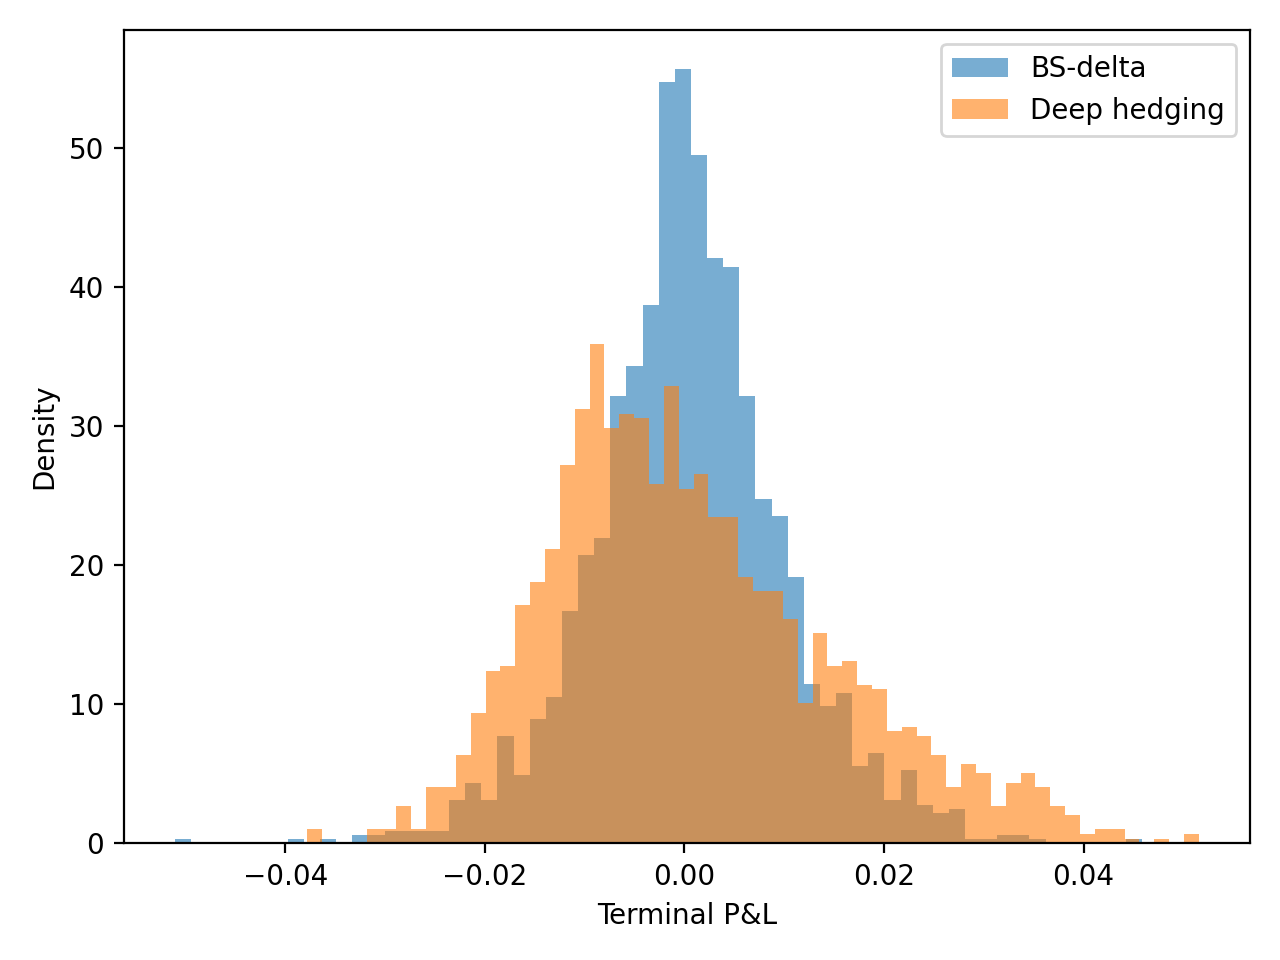
\includegraphics[width=0.85\textwidth]{figures/6_2_pl_histograms.png}
\caption{Terminal $\mathrm{P\&L}$ distributions on the GBM benchmark at
the canonical cell ($\sigma_{\mathrm{true}} = 0.20$,
$\bar\sigma = 0.20$, $\lambda = 0.0001$, oracle regime, single seed).
The Black--Scholes delta and the deep hedger produce visually
indistinguishable distributions, confirming the implementation matches
the analytical reference in the correctly-specified regime.}
\label{fig:6_2_pl_histograms}
\end{figure}

\begin{figure}[H]
\centering
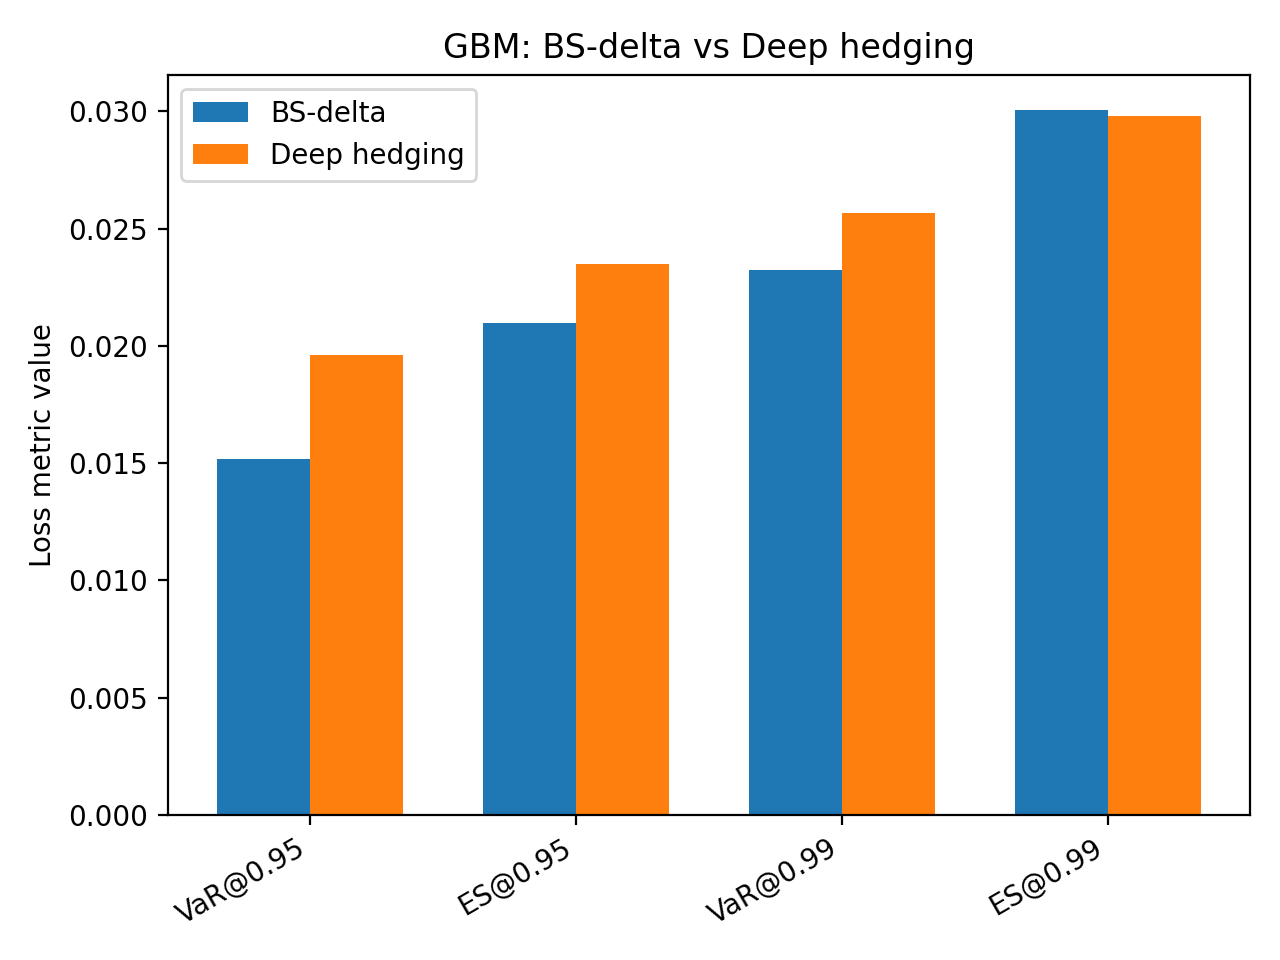
\includegraphics[width=0.85\textwidth]{figures/6_2_risk_metrics.png}
\caption{Tail-risk metrics on the GBM benchmark at the canonical cell.
$\mathrm{VaR}_{0.95}$, $\mathrm{ES}_{0.95}$, $\mathrm{VaR}_{0.99}$, and
$\mathrm{ES}_{0.99}$ are reported for the Black--Scholes delta and the
oracle deep hedger. The deep hedger marginally improves on the
analytical reference at the deeper tail levels.}
\label{fig:6_2_risk_metrics}
\end{figure}

The benchmark pipeline at the canonical cell
($\bar\sigma = 0.20$, $\lambda = 0$, oracle regime, seed $0$) reproduces
byte-identically against the canonical archived output, as documented
in Section~\ref{subsec:sim_validation}. With the deep hedging
implementation validated against the analytical reference in the
controlled GBM setting, we now turn to the rough Bergomi setting, where
all three strategies are simultaneously misspecified and no analytical
hedge is available.

\subsection{Results Under Rough Volatility}
\label{subsec:results_rough_vol}

We now turn to the rough Bergomi target setting. The data-generating
model is the differentiable rough Bergomi simulator of
Section~\ref{subsec:rb_sim} at the canonical calibration ($H = 0.07$,
$\eta = 1.9$, $\rho = -0.7$, $\xi_0 = 0.235^2$). The test set is the
frozen master set of $50{,}000$ paths simulated with seed 2024. All
three hedging strategies of Section~\ref{sec:numerical_setup} are
simultaneously misspecified in this setting. The Black--Scholes delta
ignores stochastic volatility entirely. The Heston PDE delta assumes a
Markovian variance process that is not present in the data. The deep
hedger is trained on simulated rough Bergomi paths but uses no explicit
knowledge of the underlying dynamics. The six subsections below report
the empirical results under this shared setup.

\subsubsection{Tail-risk hierarchy of hedging strategies under rough dynamics}
\label{sec:6_3_1}

The first experiment establishes the central comparison: how do the
three strategies rank on tail risk under canonical rough Bergomi
dynamics? The Heston model is calibrated by price matching to the
rough Bergomi data-generating process. We hold the leverage correlation
fixed at $\rho = -0.7$ and the initial variance at $V_0 = \xi_0 =
0.235^2 = 0.055225$, then choose the mean-reversion speed and
vol-of-vol to match the at-the-money call price under rough Bergomi to
within Monte Carlo noise. The calibration yields $\kappa = 1.0$,
$\theta = V_0 = 0.055225$, and $\sigma_v = 0.5538$. The Feller
condition $2\kappa\theta \geq \sigma_v^2$ is mildly violated (slack
$2\kappa\theta - \sigma_v^2 \approx -0.196$), but the full-truncation
Euler scheme of Proposition~\ref{prop:markovian_disc}(b) handles this
through explicit clamping. The calibration data are archived under
\path{results/heston_pde/calibration_data.json}.

The headline 5-seed comparison at $\lambda = 0$ on the canonical master
test set is reported in Table~\ref{tab:6_3_1_headline}. The deep hedger
achieves $\mathrm{ES}_{0.95} = 10.4442 \pm 0.0748$, the Black--Scholes
delta achieves $11.5921 \pm 0.0316$, and the true Heston PDE delta
achieves $13.4470 \pm 0.0857$. The ranking is
\[
  \mathrm{ES}_{0.95}^{\mathrm{DH}} \;<\; \mathrm{ES}_{0.95}^{\mathrm{BS}} \;<\; \mathrm{ES}_{0.95}^{\mathrm{Hes}}.
\]
The Heston PDE delta, despite its privileged access to the
instantaneous variance $V_t$, performs strictly worse than both the
Black--Scholes delta (which ignores $V_t$ entirely) and the deep hedger
(which observes only the spot $S_t$). The same ranking holds at the
$0.99$ confidence level, where the deep hedger achieves $\mathrm{ES}_{0.99}
= 19.0444 \pm 0.3560$ versus $21.8757 \pm 0.1636$ for the BS delta and
$19.3160 \pm 0.2286$ for the Heston PDE delta.

\begin{table}[H]
\centering
\caption{Hedging strategies under canonical rough Bergomi dynamics.
Five-seed mean $\pm$ standard deviation at $\lambda = 0$. BS delta and
deep hedger seeds 2024--2028; Heston PDE delta seeds 6024--6028. Lower
is better.}
\label{tab:6_3_1_headline}
\begin{tabular}{l c c c c}
\toprule
strategy & $\mathrm{ES}_{0.95}$ & $\mathrm{ES}_{0.99}$ & $\mathrm{std\;P\&L}$ & turnover \\
\midrule
Black--Scholes delta    & $11.5921 \pm 0.0316$ & $21.8757 \pm 0.1636$ & $4.1492 \pm 0.0312$ & $2.717 \pm 0.003$ \\
True Heston PDE delta   & $13.4470 \pm 0.0857$ & $19.3160 \pm 0.2286$ & $4.8078 \pm 0.0245$ & $6.263 \pm 0.005$ \\
Deep hedger             & $10.4442 \pm 0.0748$ & $19.0444 \pm 0.3560$ & $4.1415 \pm 0.0295$ & $1.777 \pm 0.020$ \\
\bottomrule
\end{tabular}
\end{table}

The terminal $\mathrm{P\&L}$ distributions are shown in
Figure~\ref{fig:6_3_1_pnl}. All three distributions are heavy-tailed
on the loss side, but the deep hedger's left tail is visibly lighter
than the Black--Scholes delta's, which is in turn slightly lighter than
the Heston PDE delta's. The Q-Q plots of Figure~\ref{fig:6_3_1_qq}
make the deviation from Gaussianity quantitative. The Black--Scholes
delta has the most extreme left-tail outliers (standardised quantiles
down to $-35$ at the worst path); the Heston PDE delta has the
shallowest left tail in standardised units (down to $-17$); the deep
hedger sits between (down to $-31$). The Heston PDE delta achieves
its lighter left tail at the cost of higher overall variance,
$\mathrm{std\;P\&L} = 4.81$, compared to $4.15$ for the Black--Scholes
delta and $4.14$ for the deep hedger.

\begin{figure}[H]
\centering

\includegraphics[width=\textwidth]{figures/6_3_1_pnl_histograms.png}
\caption{Terminal $\mathrm{P\&L}$ distributions under canonical rough
Bergomi (seed 2024 reference test set, $50{,}000$ paths). Vertical
dashed lines mark $-\mathrm{ES}_{0.95}$ for each strategy. The deep
hedger's left tail is visibly lighter than both diffusion-based
deltas.}
\label{fig:6_3_1_pnl}
\end{figure}

\begin{figure}[H]
\centering

\includegraphics[width=\textwidth]{figures/6_3_1_qq_plots.png}
\caption{Q-Q plots of standardised terminal $\mathrm{P\&L}$ versus the
standard normal distribution under canonical rough Bergomi (seed 2024
reference test set). The reference $y = x$ line is dashed in red.
All three strategies show heavy left tails relative to a Gaussian
reference; the Heston PDE delta is closest to Gaussian on the left,
while the Black--Scholes delta has the most extreme negative outliers.}
\label{fig:6_3_1_qq}
\end{figure}

\begin{figure}[H]
\centering

\includegraphics[width=\textwidth]{figures/6_3_1_metrics_bar.png}
\caption{Five-seed risk metrics across the three hedging strategies on
canonical rough Bergomi. The deep hedger has the lowest
$\mathrm{ES}_{0.95}$ and the lowest $\mathrm{std\;P\&L}$. The Heston
PDE delta has the lowest $\mathrm{ES}_{0.99}$ at the cost of higher
overall variance.}
\label{fig:6_3_1_metrics}
\end{figure}

The Heston PDE delta's underperformance is the central observation of
this subsection. The Heston PDE delta has access to information that
the Black--Scholes delta lacks, namely the instantaneous variance
$V_t$, and computes a hedge under variance dynamics that contain
stochastic volatility and leverage. Yet on the rough Bergomi target it
performs worse than the Black--Scholes delta. The reason is structural:
under rough Bergomi the variance process is
$V_t = \xi_0 \exp(\eta W^H_t - \tfrac12 \eta^2 t^{2H})$,
driven by fractional Brownian motion of Definition~\ref{def:volterra_driver},
while the Heston model assumes that $V_t$ mean-reverts according to a
CIR process driven by ordinary Brownian motion. The Heston delta
adapts to the observed $V_t$ under the wrong dynamics. The adaptation
amplifies tail losses more than ignoring $V_t$ entirely, as the
Black--Scholes delta does. Within the family of Markovian
stochastic-volatility deltas, no choice of parameters recovers the
rough path-dependent component of the variance evolution. Confirming
H1 in this strong form requires not only that the Black--Scholes delta
have heavier left tails than the deep hedger, but also that no
Markovian stochastic-volatility delta with privileged access to $V_t$
recovers a comparable advantage. Both conditions hold here.

When proportional costs are added ($\lambda = 0.001$, canonical
five-seed values), the ranking between the Black--Scholes delta and the
deep hedger is preserved. The Black--Scholes delta degrades to
$\mathrm{ES}_{0.95} = 12.0082 \pm 0.0324$, the deep hedger to
$10.6658 \pm 0.0389$. The absolute deep hedger advantage is preserved
at approximately $1.34$ in $\mathrm{ES}_{0.95}$ units. The cost-aware
evaluation of the Heston PDE delta is documented in
Appendix~\ref{app:detailed_perturbation} and is consistent with the
zero-cost ranking.

H1 of Section~\ref{subsec:section4_hypotheses} is confirmed in its
strong form: both Markovian baselines have heavier left tails than the
deep hedger under rough Bergomi dynamics, and the heavier-tail
inefficiency is not resolved by giving the Markovian hedger access to
the instantaneous variance. The next subsections explore where the
deep hedger's advantage comes from and how robust it is, beginning
with the role of the risk objective in
Section~\ref{sec:6_3_2}.

\begin{observation}[Tail-risk hierarchy under rough volatility]
\label{obs:6_1_hierarchy}
On canonical rough Bergomi the deep hedger achieves the lightest left
tail in $\mathrm{ES}_{0.95}$ ($10.4442 \pm 0.0748$). The
Black--Scholes delta is second ($11.5921 \pm 0.0316$). The true
Heston PDE delta, despite its privileged access to the instantaneous
variance $V_t$, is third ($13.4470 \pm 0.0857$). The variance
dynamics under rough Bergomi are not those of CIR, and adapting to
$V_t$ under the wrong dynamics amplifies tail losses more than
ignoring $V_t$ entirely. Hypothesis~H1 of
Section~\ref{subsec:section4_hypotheses} is confirmed in its strong
form: heavier left tails for both Markovian baselines, with the
inefficiency unresolved by privileged access to $V_t$.
\end{observation}

\subsubsection{The risk objective is the principal lever}
\label{sec:6_3_2}

A natural question after Section~\ref{sec:6_3_1} is which training-time
choice most affects the deep hedger's tail performance. We compare the
same architecture trained under five different risk objectives, holding
the data, the network architecture, and the optimisation protocol
fixed.

The five objectives are mean squared error (MSE), expected shortfall at
confidence levels $\alpha \in \{0.50, 0.90, 0.95, 0.99\}$, and entropic
risk. The Pareto front in
Figure~\ref{fig:6_3_2_pareto} shows the resulting trade-off between
$\mathrm{ES}_{0.95}$ and the rebalancing-cost level $\lambda$. The four
ES variants cluster within Monte Carlo noise of each other across the
tested grid. The MSE-trained hedger lies above (worse than) the ES
cluster. The entropic-trained hedger is dramatically worse.

\begin{figure}[H]
\centering
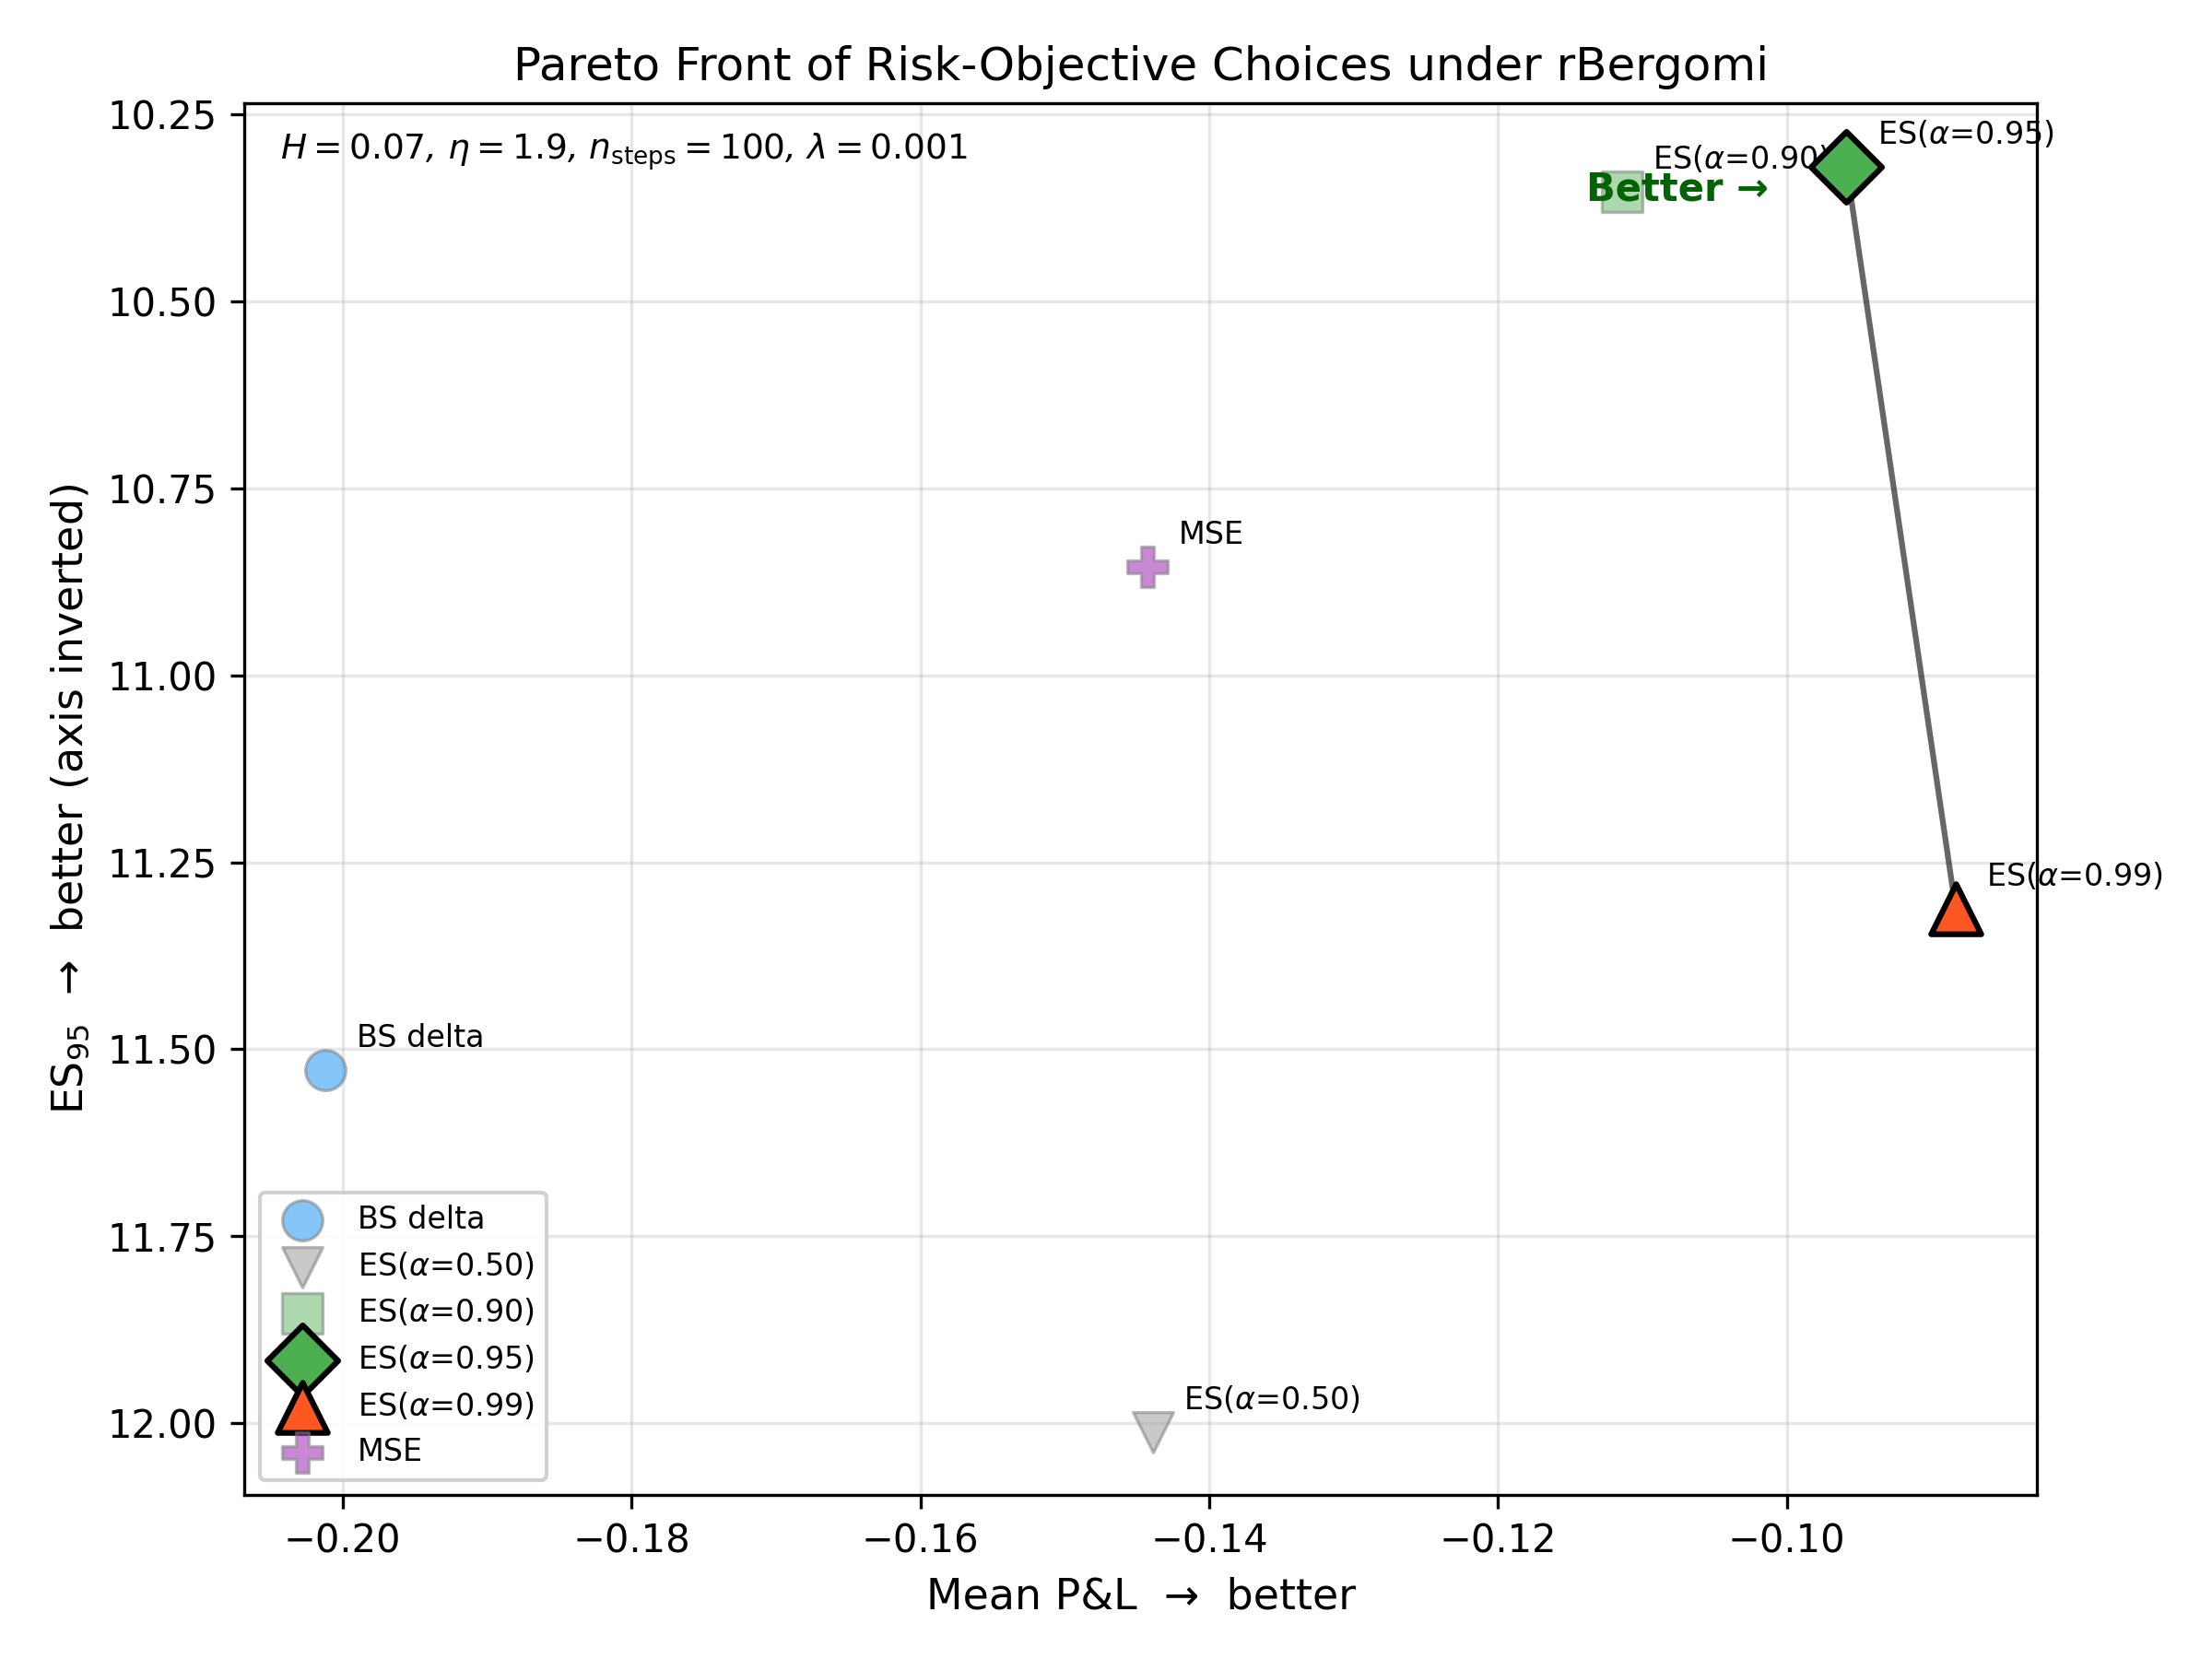
\includegraphics[width=0.85\textwidth]{figures/6_3_2_pareto_objectives.png}
\caption{Pareto front of training objectives on the canonical rough
Bergomi setting. Each point is a deep hedger trained at the indicated
rebalancing frequency $n$ and cost level $\lambda$ under one of two
objectives (here ES versus reference). The ES variants cluster within
Monte Carlo noise.}
\label{fig:6_3_2_pareto}
\end{figure}

The robustness extension stresses each objective with an axis-aligned
projected gradient attack on the rough Bergomi parameters $(H, \eta,
\rho)$ at three radii $r \in \{1, 2, 3\}$ in axis-scaled units. For
each objective, we evaluate the worst-case $\mathrm{ES}_{0.95}$ across
the six axis directions ($H \pm$, $\eta \pm$, $\rho \pm$) and aggregate
across five training seeds. The results are reported in
Table~\ref{tab:6_3_2_objective_robustness} and visualised in
Figure~\ref{fig:6_3_2_objective_robustness}. At radius $r = 1$ the
three ES variants cluster between $14.74$ and $14.90$, the MSE
objective is $0.4$ ES units above the cluster at $15.29$, and the
entropic objective is dramatically worse at $18.80$. At $r = 2$ the
same ranking holds with the entropic objective approximately $2.7$ ES
units worse than the ES cluster.

\begin{table}[H]
\centering
\caption{Worst-case $\mathrm{ES}_{0.95}$ by training objective under
axis-aligned projected gradient attacks. Each cell reports the
worst-case across six axis directions, aggregated as five-seed mean
$\pm$ standard deviation. Lower is better.}
\label{tab:6_3_2_objective_robustness}
\begin{tabular}{l c c c}
\toprule
training objective & $r = 1$ & $r = 2$ & $r = 3$ \\
\midrule
$\mathrm{ES}_{0.90}$ & $14.8426 \pm 0.5869$ & $19.1595 \pm 1.6568$ & $21.4042 \pm 1.2633$ \\
$\mathrm{ES}_{0.95}$ & $14.7380 \pm 0.6302$ & $19.1337 \pm 1.8863$ & $21.4655 \pm 1.5926$ \\
$\mathrm{ES}_{0.99}$ & $14.9043 \pm 0.4588$ & $18.9177 \pm 1.3470$ & $21.3117 \pm 1.0650$ \\
MSE                  & $15.2892 \pm 0.5029$ & $19.5253 \pm 1.4029$ & $21.7476 \pm 1.1423$ \\
Entropic             & $18.8043 \pm 1.9248$ & $21.8233 \pm 1.9102$ & $23.5681 \pm 1.5060$ \\
\bottomrule
\end{tabular}
\end{table}

\begin{figure}[H]
\centering
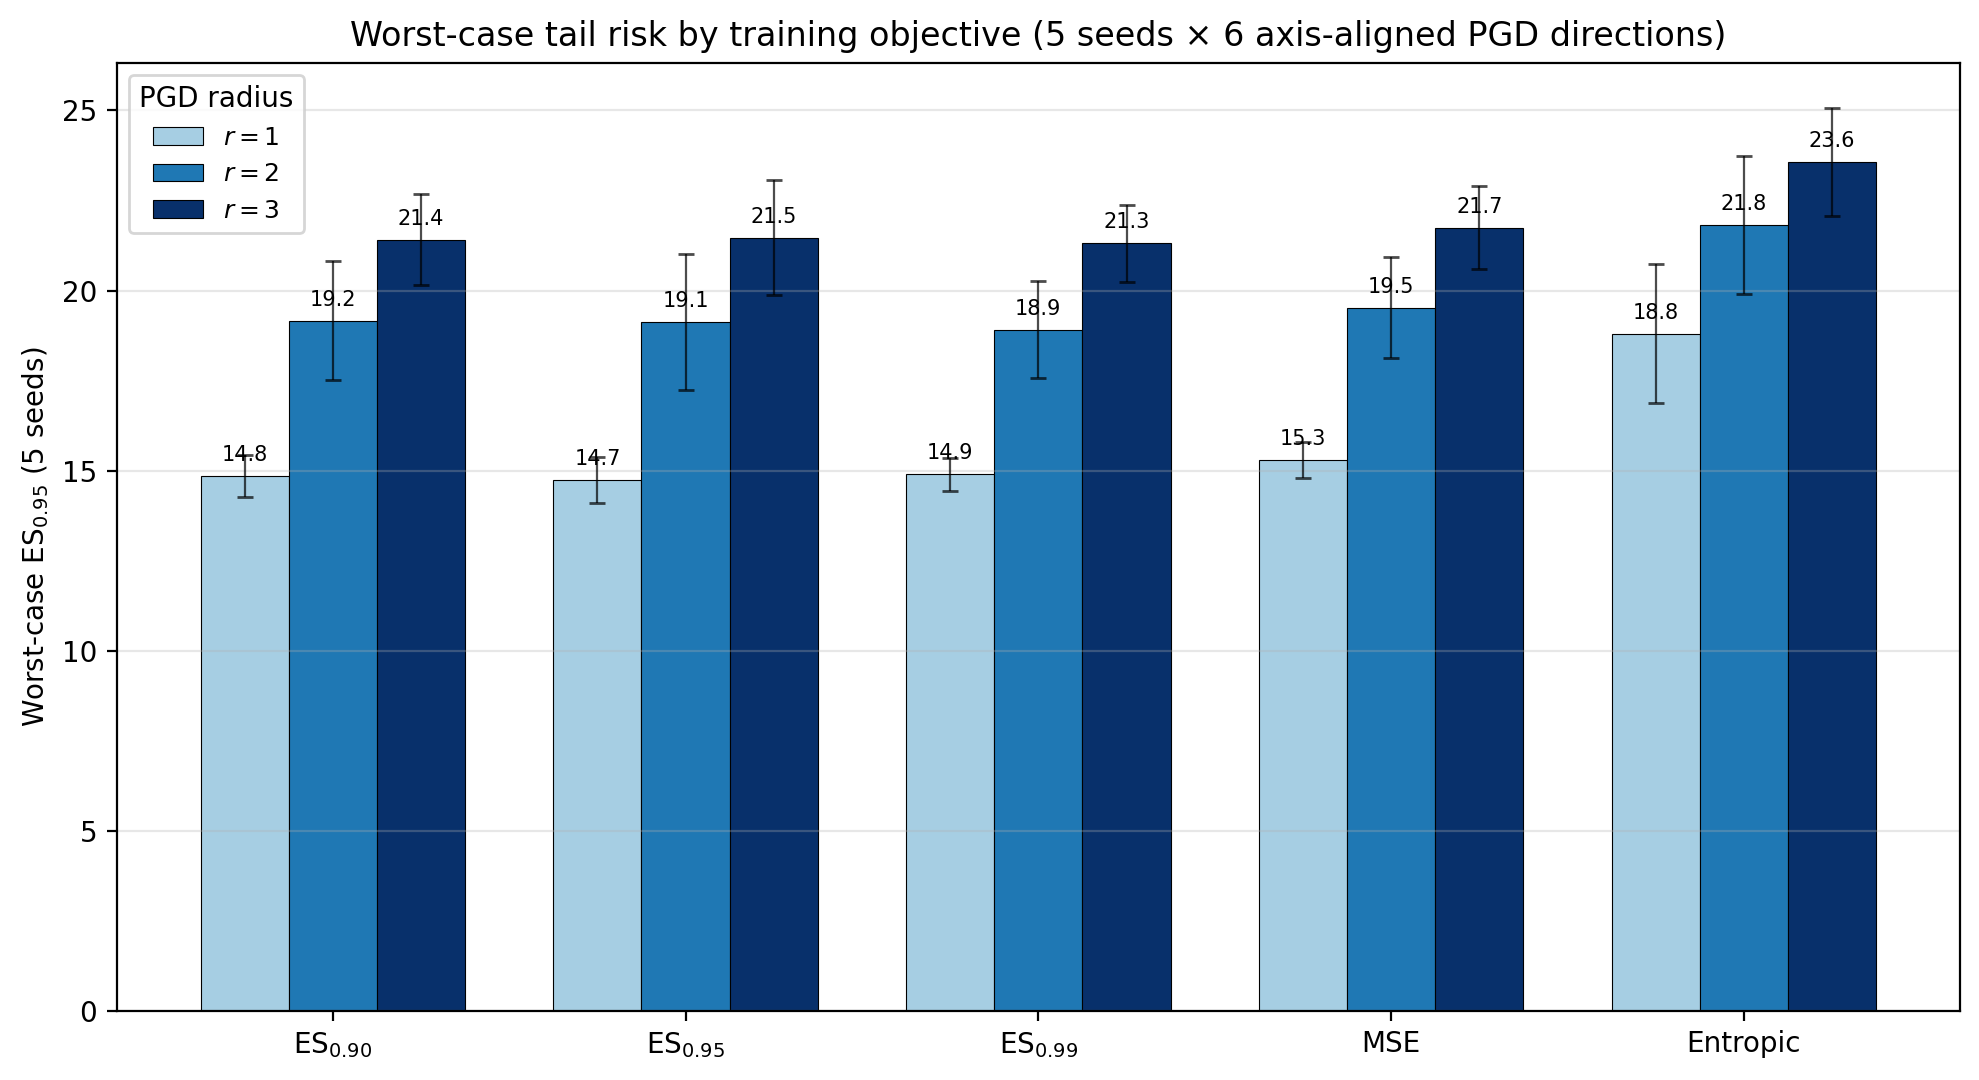
\includegraphics[width=0.95\textwidth]{figures/6_3_2_objective_robustness.png}
\caption{Worst-case $\mathrm{ES}_{0.95}$ across axis-aligned PGD
perturbation directions, by training objective and radius. The four
ES variants cluster at every radius; the MSE objective is consistently
$\sim 0.4$ ES units above the cluster; the entropic objective is
dramatically inferior at every radius.}
\label{fig:6_3_2_objective_robustness}
\end{figure}

The methodological recommendation is direct. Within the ES family the
specific confidence level $\alpha$ does not significantly affect tail
performance. The principal axis is the choice between CVaR-style
(expected shortfall) and entropic objectives. The entropic objective
should be avoided for tail-risk hedging in this regime. The MSE
objective, while worse than ES, is much closer to ES than entropic and
is acceptable when a smooth pointwise-replication objective is
preferred. The choice of risk objective is the principal training-time
lever for tail performance, and within ES variants the choice is
essentially indifferent. This finding is independent of the four
hypotheses of Section~\ref{subsec:section4_hypotheses} and supplements
them as a methodological observation.

\begin{observation}[Risk objective is the principal training-time lever]
\label{obs:6_2_objective}
Within the family of expected-shortfall objectives ($\mathrm{ES}_{0.90}$,
$\mathrm{ES}_{0.95}$, $\mathrm{ES}_{0.99}$), the specific confidence
level $\alpha$ does not significantly affect tail performance. The
objectives cluster within Monte Carlo noise across the perturbation
grid. The mean squared error objective is approximately $0.4$
$\mathrm{ES}_{0.95}$ units above the cluster. The entropic objective
is dramatically inferior at every tested radius, by approximately
$3$ $\mathrm{ES}_{0.95}$ units. The principal methodological
recommendation is to use any expected-shortfall variant for
tail-aware deep hedging and to avoid the entropic objective in this
regime.
\end{observation}

\subsubsection{What roughness does and does not do}
\label{sec:6_3_3}

We now turn to H4 of Section~\ref{subsec:section4_hypotheses}. The
hypothesis claims that a flat-feature deep hedger captures the
principal advantage without exploiting the path-dependent structure of
the rough variance process. Three independent experiments speak to
this claim: a sweep of the deep hedger's advantage as a function of
the Hurst parameter $H$, a signature-feature ablation at three Hurst
values, and a cross-axis comparison of the deep hedger's $\mathrm{ES}_{0.95}$
sensitivity to the roughness exponent $H$ versus the
stochastic-volatility level $\eta$.

The first experiment varies $H$ across the range $[0.01, 0.50]$ at
nine grid points, holding the other rough Bergomi parameters fixed at
$\eta = 1.9$, $\rho = -0.7$, $\xi_0 = 0.235^2$. At each $H$ a deep
hedger is trained from scratch and evaluated on a $50{,}000$-path test
set drawn from the same parameter setting, with the Black--Scholes
delta as a reference. The deep hedger's advantage
$\Gamma(H) = \mathrm{ES}_{0.95}^{\mathrm{BS}}(H) - \mathrm{ES}_{0.95}^{\mathrm{DH}}(H)$
is plotted in Figure~\ref{fig:6_3_3_h_sweep}. A power-law fit
$\log \Gamma(H) = \alpha + \beta \log H$ yields the panel-OLS slope
estimate
\[
  \hat\beta = 0.014 \;\pm\; 0.022,
  \qquad
  \text{$95\%$ bootstrap CI}\; [-0.073, +0.088],
\]
with $10{,}000$ bootstrap samples. The bootstrap noise floor at the
prevailing Monte Carlo standard error is $\beta_{\mathrm{noise}} =
0.663$. The ratio
$|\hat\beta| / \beta_{\mathrm{noise}} = 0.021$
places the slope deep in the noise regime, more than an order of
magnitude below what the seed-to-seed Monte Carlo error alone would
produce. The advantage is statistically flat across the range of
Hurst values considered.

\begin{figure}[H]
\centering
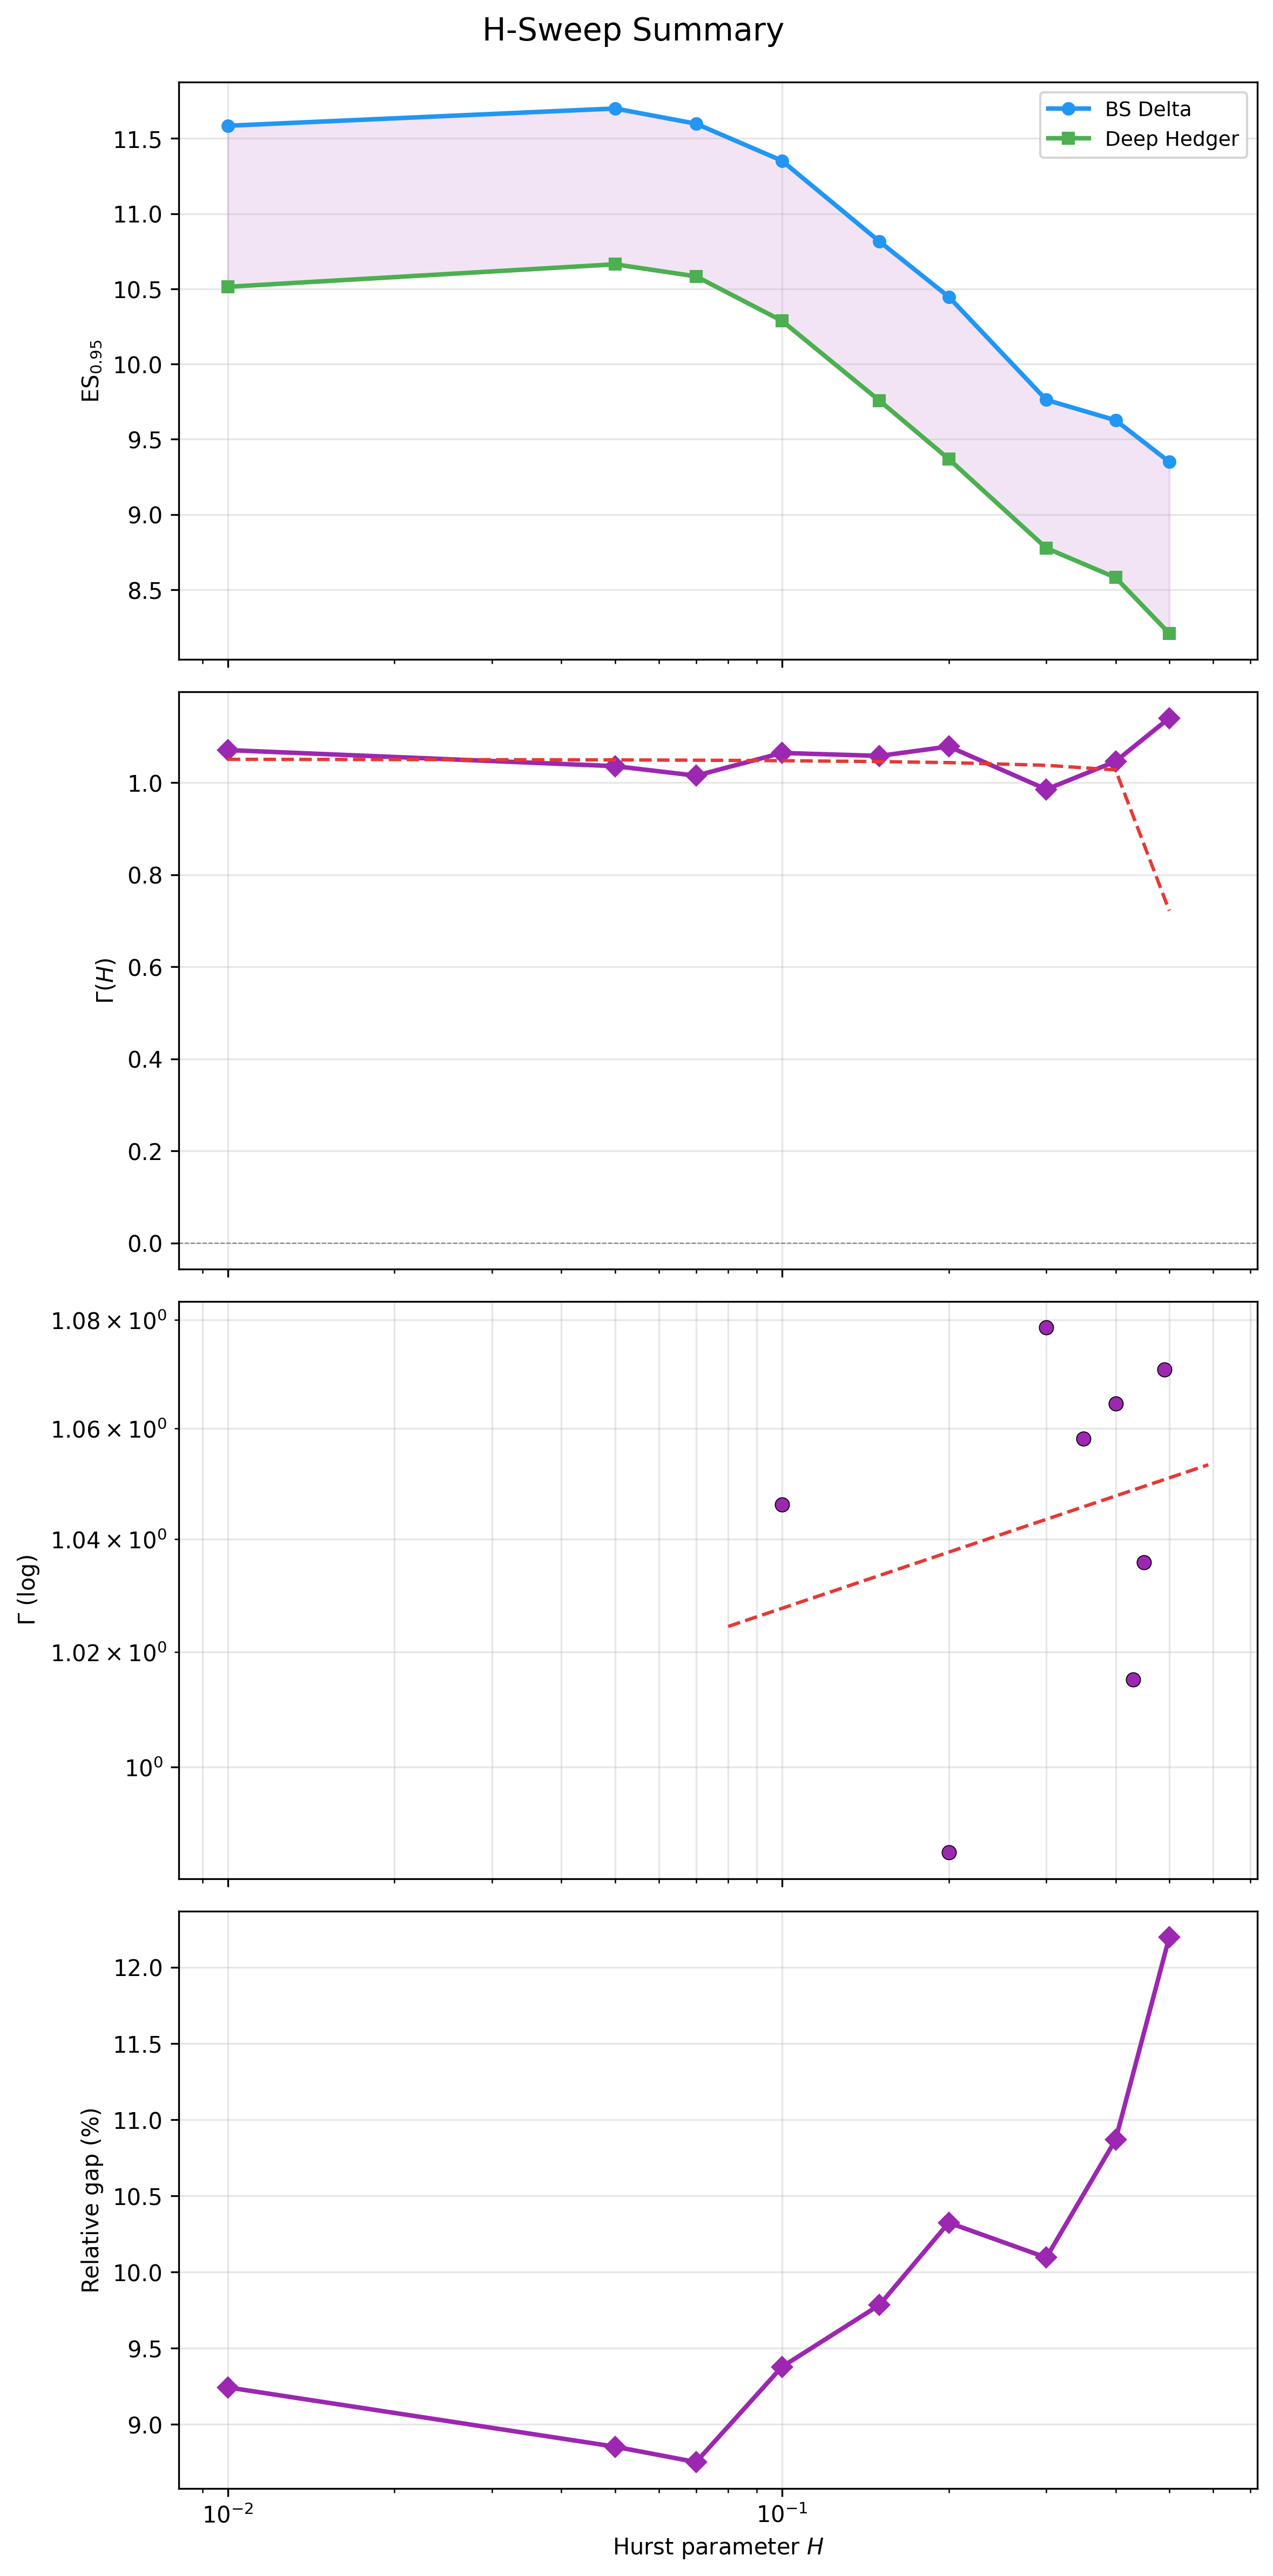
\includegraphics[width=0.8\textwidth]{figures/6_3_3_h_sweep.png}
\caption{Roughness sweep: deep hedger advantage $\Gamma(H)$ versus
Hurst parameter on a log--log scale, at nine grid points across the
range $[0.01, 0.50]$. The fitted slope $\hat\beta = 0.014 \pm 0.022$
($95\%$ bootstrap CI $[-0.073, +0.088]$) is statistically
indistinguishable from zero against the noise floor $\beta_{\mathrm{noise}}
= 0.663$.}
\label{fig:6_3_3_h_sweep}
\end{figure}

The second experiment is a signature-feature ablation at three Hurst
values $H \in \{0.02, 0.05, 0.25\}$. The flat-feature deep hedger of
Section~\ref{subsec:deep_hedging_framework} (input dimension 4) is
compared to a deep hedger augmented with a 3-dimensional truncated
log-signature (input dimension 7) and a deep hedger augmented with a
12-dimensional full path-feature vector (input dimension 16). The
augmented features include realised variance at three lookback
horizons, drawdown, range, quadratic variation, and additional
signature components, all features that, in principle, encode the
path-dependent structure of the rough variance process. At every
tested $H$, neither augmentation produces a positive
$\Gamma_{\mathrm{aug}} - \Gamma_{\mathrm{flat}}$. The mean
augmentation effect across $H$ is negative. Five remediation
strategies (extended training budget, two-tower architecture,
learning-rate warm-up, feature standardisation, permutation importance
analysis) all fail to recover positive signal.

The third experiment compares the deep hedger's $\mathrm{ES}_{0.95}$
sensitivity along the $H$ axis versus the $\eta$ axis. Holding the
other parameters at the canonical values, we evaluate the deep hedger
on $15$ grid points spanning $H \in [0.02, 0.17]$ and on $15$ grid
points spanning $\eta \in [0.4, 3.4]$. The standard deviation of the
deep hedger's $\mathrm{ES}_{0.95}$ across the $15$ points is
\[
  \mathrm{std}_{\eta} \;=\; 5.19,
  \qquad
  \mathrm{std}_{H} \;=\; 0.40,
  \qquad
  \mathrm{std}_{\eta} / \mathrm{std}_{H} \;\approx\; 13.0.
\]
The deep hedger's $\mathrm{ES}_{0.95}$ varies by approximately $13$
times more along the stochastic-volatility level axis than along the
roughness axis. The two-dimensional $(H, \eta)$ heatmap of
Figure~\ref{fig:6_3_3_h_eta_grid} visualises the asymmetry: the
horizontal $H$ slices are nearly flat, while the vertical $\eta$
slices vary sharply.

\begin{figure}[H]
\centering
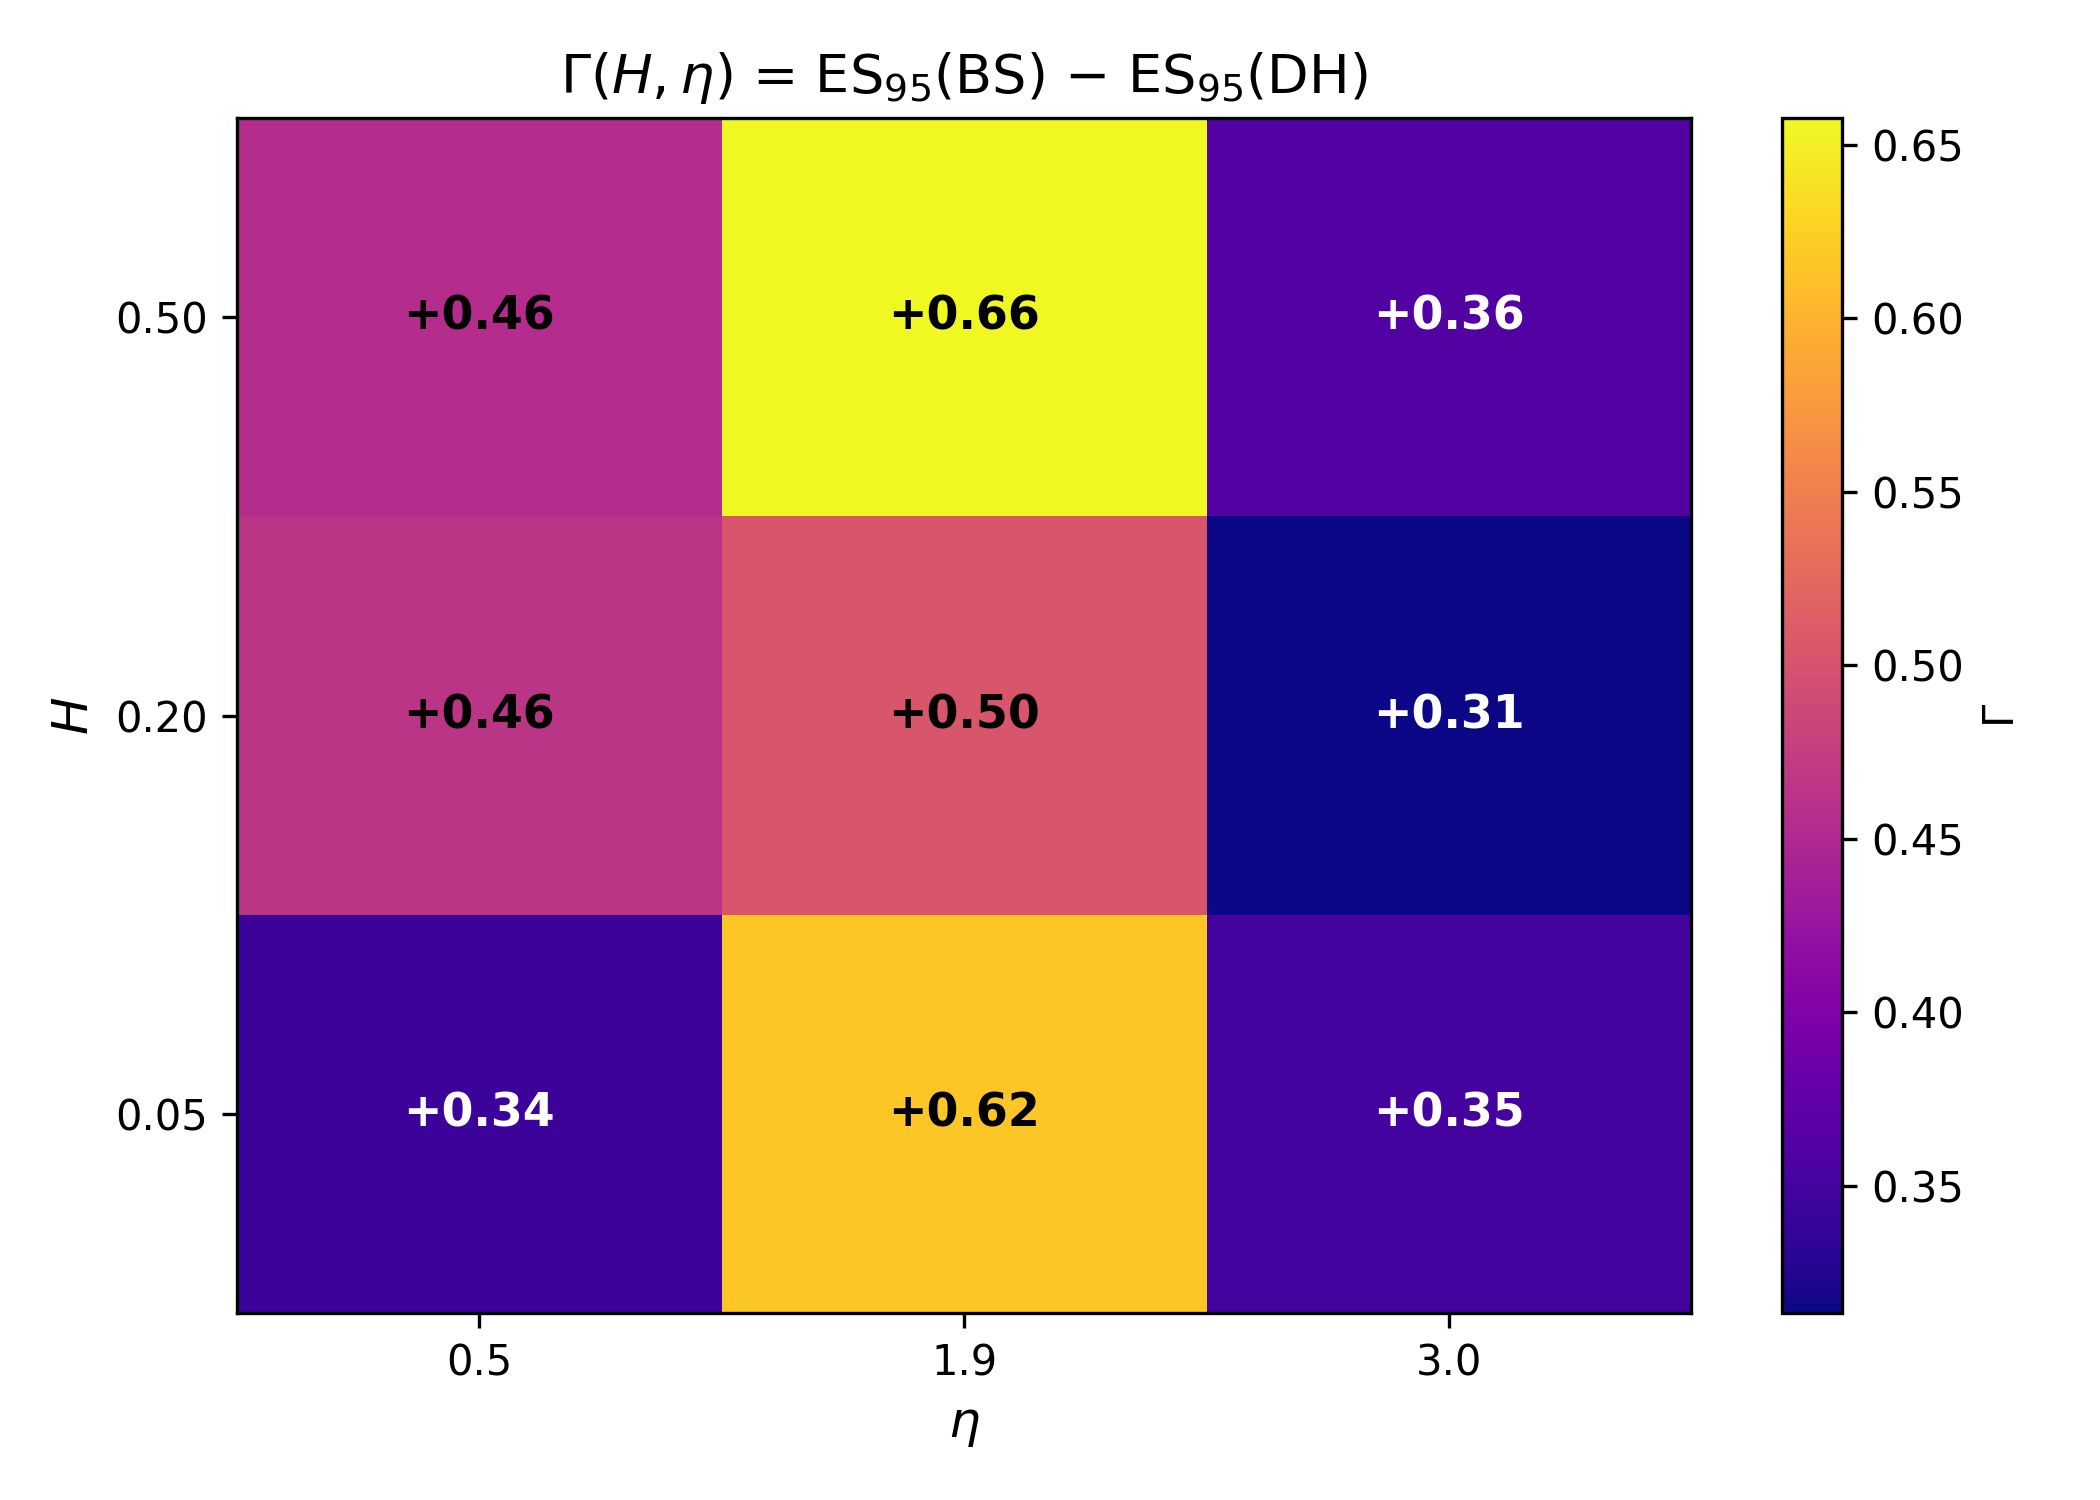
\includegraphics[width=0.75\textwidth]{figures/6_3_3_H_eta_grid.png}
\caption{Two-dimensional heatmap of the deep hedger's
$\mathrm{ES}_{0.95}$ across the $(H, \eta)$ grid. The horizontal $H$
slices are nearly flat. The vertical $\eta$ slices show strong
variation. The standard deviation of the deep hedger's
$\mathrm{ES}_{0.95}$ across the $\eta$ axis is approximately $13$
times the standard deviation across the $H$ axis.}
\label{fig:6_3_3_h_eta_grid}
\end{figure}

The three experiments converge on the same conclusion. The roughness
parameter $H$ does not modulate the deep hedger's advantage; the
advantage is statistically flat in $H$, and signature features that
encode path-dependent structure do not help. The relevant axis is the
stochastic-volatility level $\eta$. H4 is confirmed in its strong
form: flat features suffice for the principal advantage, and the deep
hedger's basin of advantage is parameterised by $\eta$ rather than by
$H$.

\begin{observation}[Roughness is not the source of the advantage]
\label{obs:6_3_roughness}
Three independent experiments confirm that the deep hedger's
advantage is not modulated by the roughness exponent $H$. The
advantage $\Gamma(H)$ is statistically flat across $H \in [0.01,
0.50]$, with panel-OLS slope $\hat\beta = 0.014 \pm 0.022$ and
$|\hat\beta| / \beta_{\mathrm{noise}} = 0.021$, deep in the noise
regime. Signature features that encode path-dependent structure do
not improve over flat features at any tested Hurst value. The deep
hedger's $\mathrm{ES}_{0.95}$ varies approximately $13$ times more
along the stochastic-volatility level $\eta$ than along the
roughness $H$. Hypothesis~H4 of
Section~\ref{subsec:section4_hypotheses} is confirmed: flat features
suffice, and the relevant axis is $\eta$, not $H$.
\end{observation}

\subsubsection{Cross-model transferability}
\label{sec:6_3_4}

Section~\ref{sec:6_3_3} identified the roughness parameter $H$ as not
modulating the deep hedger's advantage. A natural follow-up question
asks whether the deep hedging policy itself transfers across data-generating
models. We report three transfer experiments. The forward transfer
trains the deep hedger on simpler source dynamics and evaluates
zero-shot on the canonical rough Bergomi target. The reverse transfer
trains on rough Bergomi and evaluates on simpler Markovian targets. The
cross-calibration transfer evaluates the canonical hedger across other
Hurst values within the rough Bergomi family.

In the forward direction we test three sources: GBM with constant
volatility $0.235$, the calibrated Heston model of Section~\ref{sec:6_3_1},
and a rough Bergomi at $H = 0.3$ that is moderately rough but distinct
from the canonical $H = 0.07$. For each source, a deep hedger is
trained from scratch on the source paths and then evaluated zero-shot
on the canonical rough Bergomi master test set. The Heston source is
evaluated across five training seeds; the GBM and rough Bergomi at
$H = 0.3$ sources are evaluated across three training seeds drawn from
the budget sweep (training set size $N = 160{,}000$). The five-seed
canonical Black--Scholes delta and the five-seed canonical deep hedger
are reference baselines. Results are reported in
Table~\ref{tab:6_3_4_multi_source} and visualised in
Figure~\ref{fig:6_3_4_multi_source}.

\begin{table}[H]
\centering
\caption{Multi-source zero-shot transfer to the canonical rough
Bergomi target. Each row reports $\mathrm{ES}_{0.95}$ on the canonical
$50{,}000$-path test set under a hedger trained on the indicated
source. The Heston source uses five training seeds; the GBM and
$H = 0.3$ sources use three seeds drawn from the budget sweep at
$N = 160{,}000$ training paths. Lower is better.}
\label{tab:6_3_4_multi_source}
\begin{tabular}{l c}
\toprule
training source & $\mathrm{ES}_{0.95}$ \\
\midrule
GBM ($\sigma = 0.235$, 3 seeds)                          & $11.0791 \pm 0.0106$ \\
Heston (calibrated, 5 seeds)                             & $10.4431 \pm 0.0256$ \\
Rough Bergomi at $H = 0.3$ (3 seeds)                     & $10.5488 \pm 0.0353$ \\
\midrule
Reference: Black--Scholes delta (5 seeds)                & $11.5921 \pm 0.0316$ \\
Reference: canonical deep hedger (5 seeds)               & $10.4442 \pm 0.0748$ \\
\bottomrule
\end{tabular}
\end{table}

\begin{figure}[H]
\centering
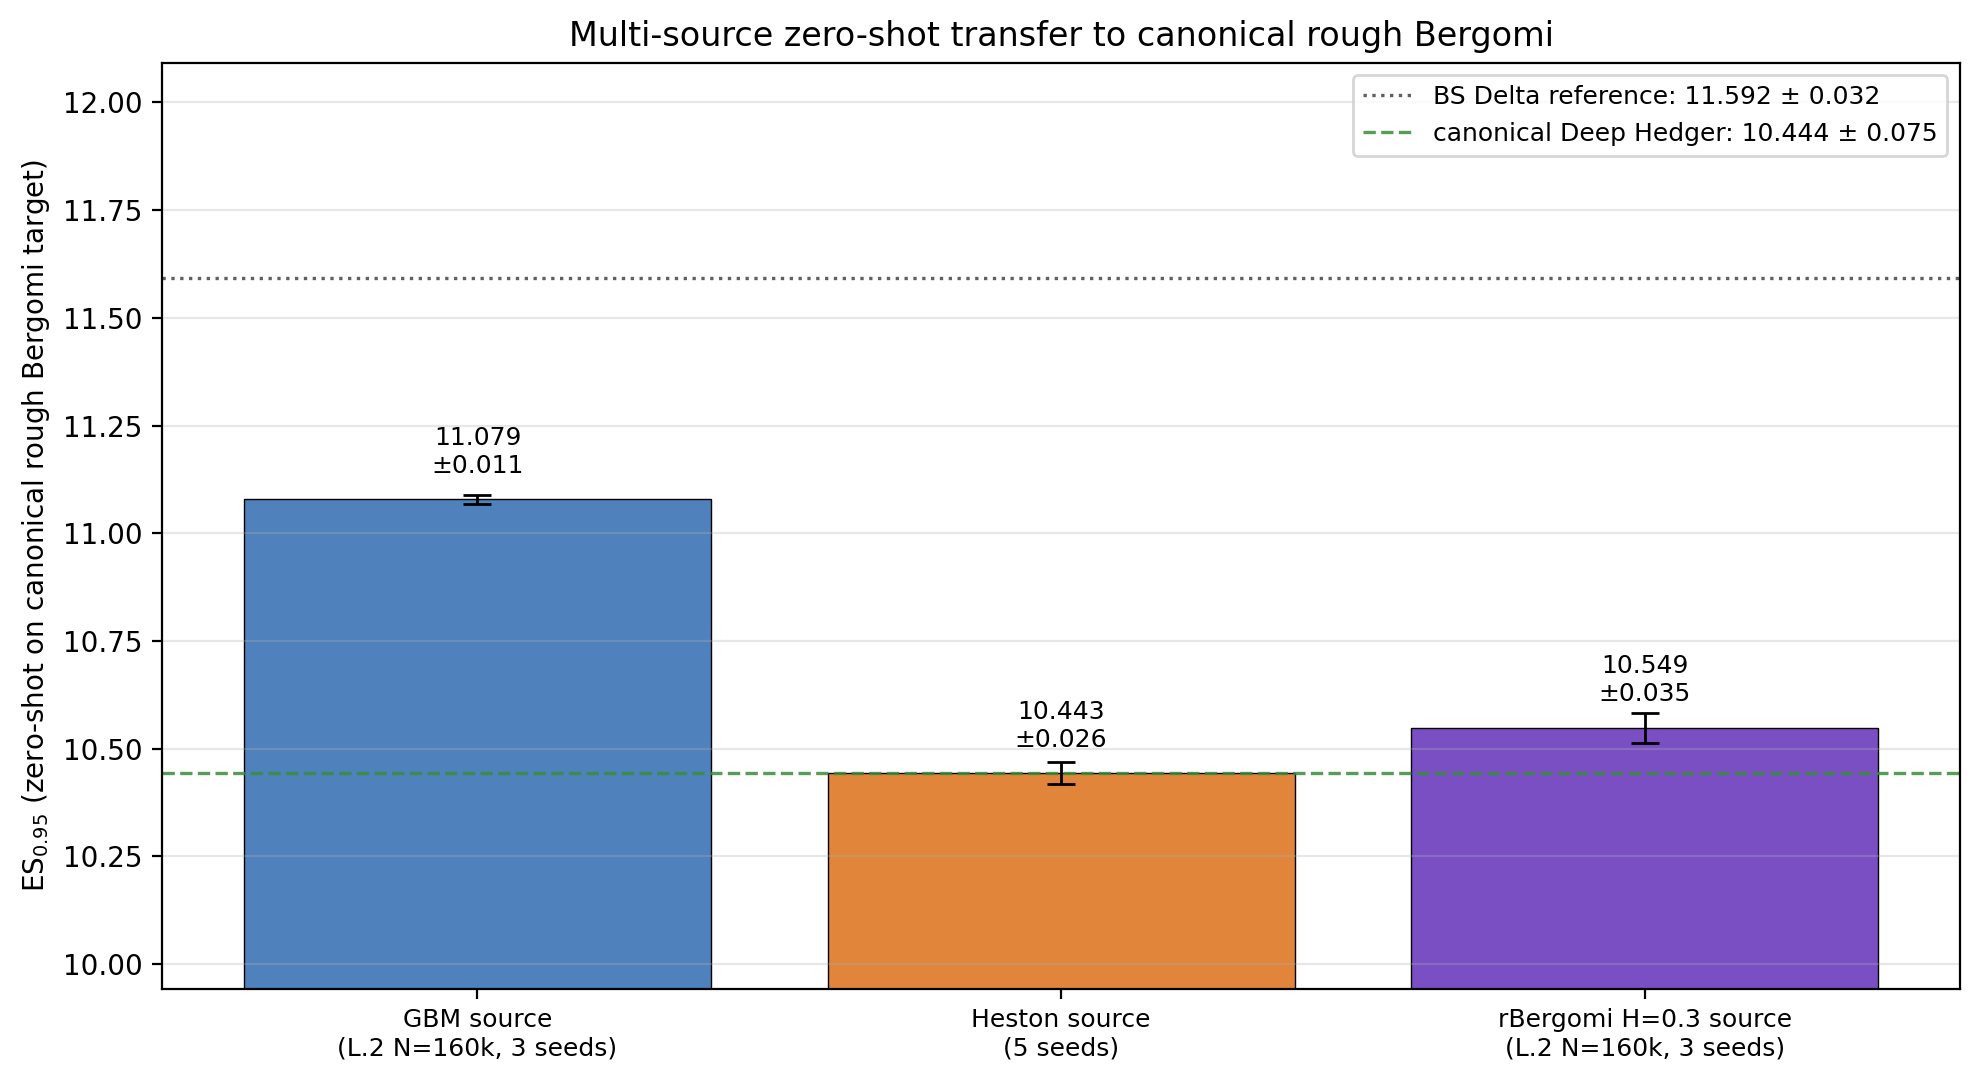
\includegraphics[width=0.95\textwidth]{figures/6_3_4_multi_source.png}
\caption{Multi-source zero-shot transfer to canonical rough Bergomi.
Bars show training-source $\mathrm{ES}_{0.95}$ on the canonical test
set. Reference lines show the canonical Black--Scholes delta (dotted)
and the canonical deep hedger (dashed). The Heston-source error band
overlaps the canonical deep hedger reference line.}
\label{fig:6_3_4_multi_source}
\end{figure}

The Heston-source deep hedger achieves
$\mathrm{ES}_{0.95} = 10.4431 \pm 0.0256$, statistically
indistinguishable from the canonical deep hedger
$\mathrm{ES}_{0.95} = 10.4442 \pm 0.0748$ that was trained directly on
rough Bergomi paths. The pooled gap is $-0.0011$ ES units, more than
two orders of magnitude smaller than the seed-to-seed standard
deviation. The Heston-trained hedger achieves canonical performance on
rough Bergomi without ever seeing a rough Bergomi path during training.
The rough Bergomi at $H = 0.3$ source achieves $10.5488 \pm 0.0353$,
within $0.10$ ES units of the canonical deep hedger. The GBM source
achieves $11.0791 \pm 0.0106$, beating the Black--Scholes reference
($11.5921$) but not reaching the canonical deep hedger. The pattern is
that source models with stochastic variance and leverage (Heston, rough
Bergomi at $H = 0.3$) transfer essentially perfectly. The
constant-volatility GBM source transfers partially.

The reverse transfer is asymmetric. We take the canonical
rough-Bergomi-trained deep hedger and evaluate it zero-shot on
Markovian targets. The two targets are GBM at $\sigma = 0.20$, where
the analytical reference is the Black--Scholes delta, and the
calibrated Heston model, where the analytical reference is the Heston
PDE delta. Results are reported in
Table~\ref{tab:6_3_4_reverse} and visualised in
Figure~\ref{fig:6_3_4_reverse_transfer}. On the Heston target, the
rough-Bergomi-trained deep hedger achieves
$\mathrm{ES}_{0.95} = 7.37 \pm 0.07$, compared to the Heston PDE
delta's $9.47 \pm 0.07$. The rB-trained hedger \emph{beats} the Heston
PDE on Heston paths, with a gap of $-2.11 \pm 0.11$. On the GBM target,
the rB-trained hedger achieves $\mathrm{ES}_{0.95} = 3.95 \pm 0.03$,
compared to the Black--Scholes delta's $1.89 \pm 0.03$. The rB-trained
hedger \emph{loses} to the BS delta on GBM, with a gap of
$+2.07 \pm 0.01$. The asymmetry is structural: forward transfer
"downhill in complexity" (Heston source, rough Bergomi target) succeeds.
Reverse transfer "uphill in simplicity" (rough Bergomi source, GBM
target) fails.

\begin{table}[H]
\centering
\caption{Reverse transfer of the canonical rough-Bergomi-trained deep
hedger to Markovian targets. Each row reports the deep hedger's
$\mathrm{ES}_{0.95}$ on the indicated target test set, the analytical
reference, and the gap. Three seeds.}
\label{tab:6_3_4_reverse}
\begin{tabular}{l c c c}
\toprule
target & rB-DH $\mathrm{ES}_{0.95}$ & reference $\mathrm{ES}_{0.95}$ & gap \\
\midrule
GBM ($\sigma = 0.20$)        & $3.9541 \pm 0.0300$ & $1.8865 \pm 0.0321$ (BS)         & $+2.0676 \pm 0.0083$ \\
Heston (calibrated)          & $7.3681 \pm 0.0720$ & $9.4732 \pm 0.0674$ (Heston PDE) & $-2.1051 \pm 0.1057$ \\
\bottomrule
\end{tabular}
\end{table}

\begin{figure}[H]
\centering
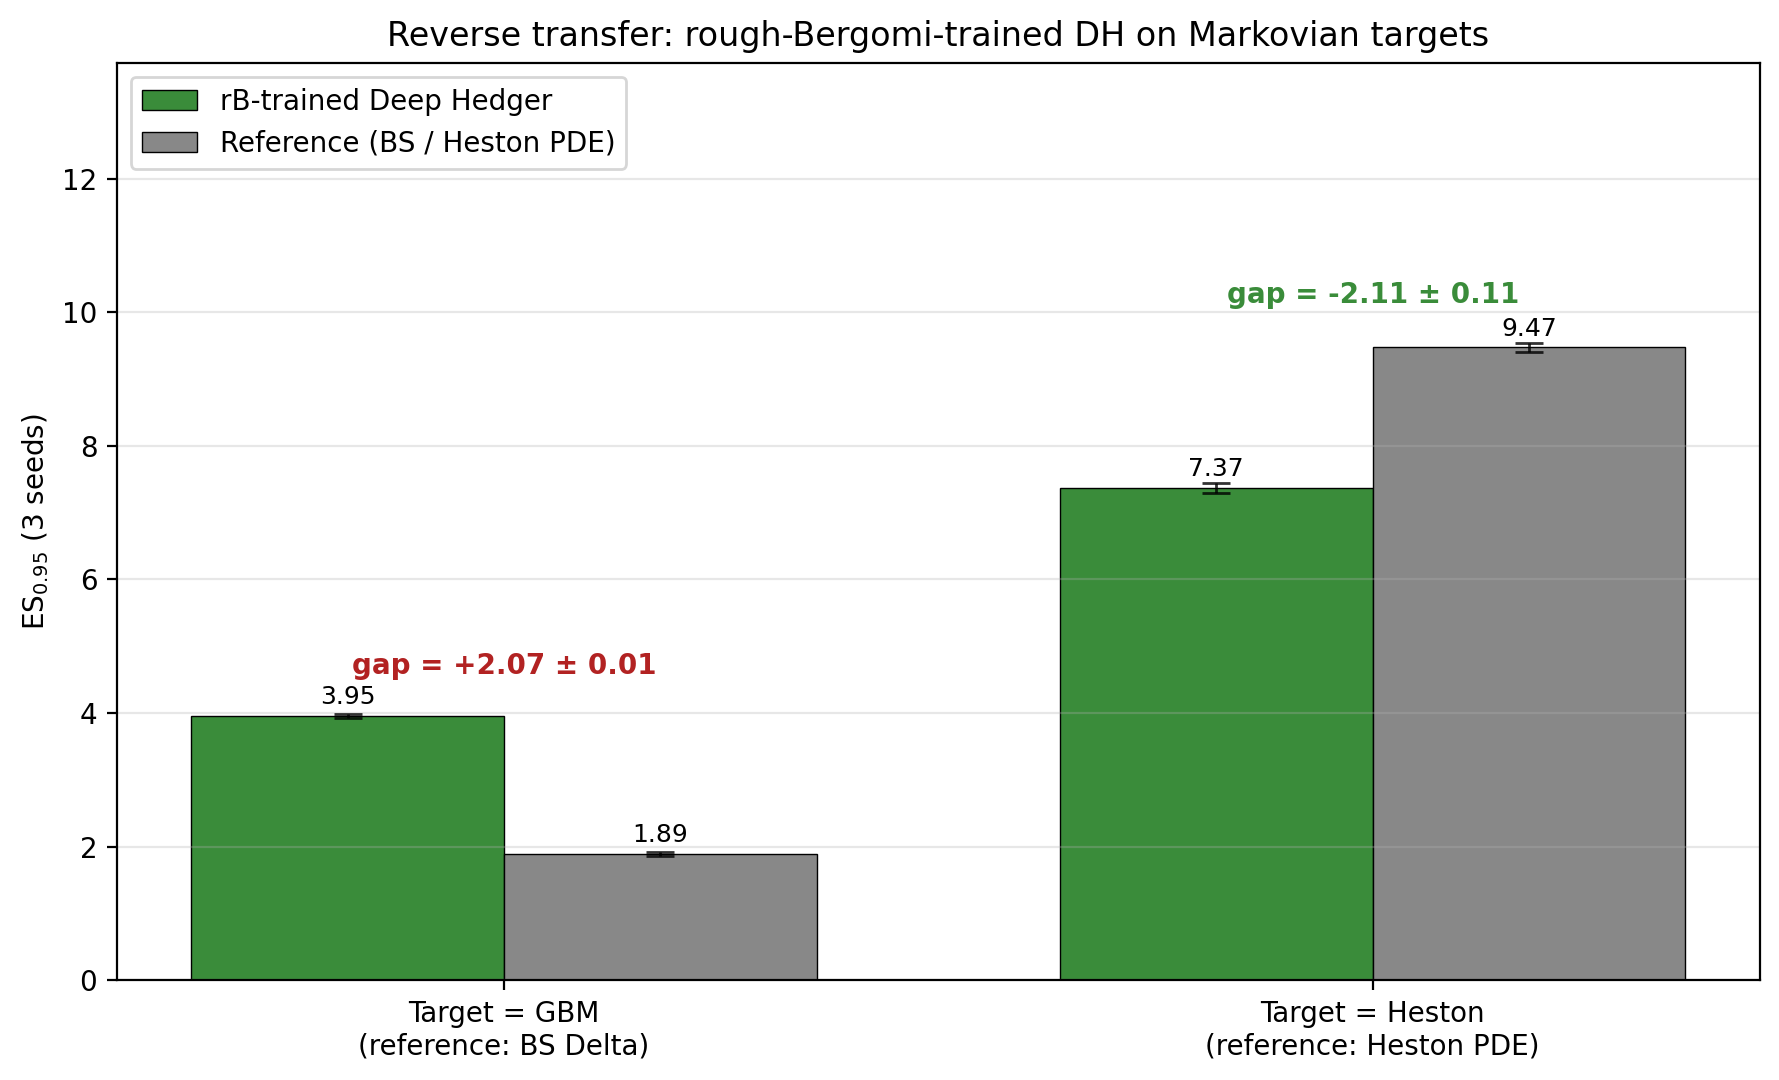
\includegraphics[width=0.95\textwidth]{figures/6_3_4_reverse_transfer.png}
\caption{Reverse transfer: canonical rough-Bergomi-trained deep hedger
on Markovian targets. On the Heston target, the deep hedger beats the
Heston PDE reference by $2.11$ ES units. On the GBM target, the deep
hedger loses to the Black--Scholes reference by $2.07$ ES units.}
\label{fig:6_3_4_reverse_transfer}
\end{figure}

The third experiment evaluates the canonical hedger at three Hurst
values within the rough Bergomi family. Holding $\eta$, $\rho$, and
$\xi_0$ fixed at the canonical values, the canonical-trained deep
hedger is applied to test sets at $H \in \{0.07, 0.20, 0.40\}$. The
deep hedger advantage shrinks with calibration distance from the
training point: at $H = 0.07$ the gap is $-1.15 \pm 0.09$ ES units; at
$H = 0.20$ the gap is $-1.06 \pm 0.05$; at $H = 0.40$ the gap is
$-0.87 \pm 0.05$. The advantage gap shrinks gracefully with
calibration distance but never crosses zero across the tested Hurst
range. The full curve is documented in
Appendix~\ref{app:detailed_transfer}.

The reverse-transfer-to-GBM failure mode points to a specific
boundary. The rough-Bergomi-trained hedger has learned a hedging
policy adapted to the canonical level of stochastic volatility
$\eta = 1.9$. On GBM, where the effective variance is constant, the
policy over-reacts to spurious variance signals and produces a hedge
worse than the constant-volatility analytical reference. The
fine-grained $\eta$-axis behaviour and the broader robustness of the
canonical-trained policy are the subject of
Section~\ref{sec:6_3_5}.

A final transfer-related observation concerns fine-tuning. When the
GBM-source deep hedger is fine-tuned on small samples of rough Bergomi
data, the resulting policy is worse than the zero-shot transfer at
every fine-tuning sample size we tested in $[100, 80{,}000]$. The
zero-shot GBM-source baseline achieves
$\mathrm{ES}_{0.95} = 11.09$; fine-tuning at any sample size yields a
worse $\mathrm{ES}_{0.95}$. This is a form of catastrophic forgetting:
small rough-Bergomi gradients destabilise the GBM-source policy
without producing enough rough-Bergomi-specific adaptation to recover.
The detailed fine-tuning curve is in
Appendix~\ref{app:detailed_transfer}.

The transferability picture is structured. Forward transfer broadly
works across source models that have stochastic variance and leverage.
Within the rough Bergomi family the canonical-trained hedger
generalises across $H$ values without re-training. Reverse transfer
is asymmetric: the rB-trained hedger preserves richness on Heston but
fails on GBM. Fine-tuning from a GBM-source policy makes things
worse, not better. H3 of Section~\ref{subsec:section4_hypotheses} is
partially confirmed in the cross-calibration sense within the rough
Bergomi family, with the $\eta \to 0$ boundary identified as the limit
of the dynamics-agnostic regime.

\begin{observation}[Asymmetric cross-model transfer with bounded basin]
\label{obs:6_4_transfer}
Forward zero-shot transfer to canonical rough Bergomi works broadly
across source models with stochastic variance and leverage. The
Heston-source deep hedger achieves canonical performance
($10.4431 \pm 0.0256$ versus canonical $10.4442 \pm 0.0748$,
statistically indistinguishable) without ever seeing a rough Bergomi
path during training. Reverse transfer is asymmetric. The
rough-Bergomi-trained hedger beats the Heston PDE on Heston paths
but loses to the Black--Scholes delta on GBM paths. Within the rough
Bergomi family, cross-calibration is robust: the advantage gap
shrinks gracefully across $H \in \{0.07, 0.20, 0.40\}$ and never
crosses zero. The basin of advantage is bounded by the Markovian
limit $\eta \to 0$.
\end{observation}

\subsubsection{Frequency--cost interaction and parameter perturbation}
\label{sec:6_3_5}

This subsection tests two hypotheses jointly. H2 of
Section~\ref{subsec:section4_hypotheses} states that under sufficient
proportional cost, increasing the rebalancing frequency strictly
worsens tail metrics. H3 states that the deep hedger's absolute
advantage persists uniformly under axis-aligned and worst-case
parameter perturbations. The first half of the subsection treats
the frequency--cost interaction (H2). The second half treats the
parameter-perturbation robustness of the canonical-trained hedger
(H3).

\paragraph{Frequency--cost interaction.}

The frequency--cost trade-off concerns the choice of rebalancing
frequency $n$ under a proportional cost coefficient $\lambda$. We
evaluate the Black--Scholes delta and the cost-aware Leland delta on a
grid where the rebalancing frequency $n$ ranges over the values
$25$, $50$, $100$, $200$, $400$, and $800$, and the cost coefficient
$\lambda$ ranges over
$0$, $5 \cdot 10^{-4}$, $10^{-3}$, $2 \cdot 10^{-3}$,
$3 \cdot 10^{-3}$, $5 \cdot 10^{-3}$, and $10^{-2}$, on the canonical
rough Bergomi master test set ($N = 50{,}000$). At each cost level we
record the resulting $\mathrm{ES}_{0.95}$ across the six rebalancing
frequencies and compute the Kendall rank correlation $\tau_n$ between
$n$ and $\mathrm{ES}_{0.95}$. A negative $\tau_n$ indicates that more
frequent rebalancing reduces tail risk; a positive $\tau_n$ indicates
the reverse.

The Kendall correlations for the Black--Scholes delta are reported in
Table~\ref{tab:6_3_5_kendall}. At zero cost and the smallest
non-trivial cost levels (up to $\lambda = 10^{-3}$), the correlation is
$\tau_n = -1$, meaning $\mathrm{ES}_{0.95}$ decreases monotonically as
$n$ grows. The optimal frequency $n^*$ is the maximum tested value
($800$). At $\lambda = 2{\cdot}10^{-3}$ the correlation rises to
$-0.87$ and the optimum shifts to $n^* = 400$. By $\lambda = 5{\cdot}10^{-3}$
the correlation has nearly collapsed ($\tau_n = -0.07$) and the
optimum is at $n^* = 100$. At $\lambda = 10^{-2}$ the correlation
reverses sign to $\tau_n = +0.47$, with the optimum at $n^* = 100$.
The crossover from monotonic improvement to monotonic deterioration
occurs at a cost threshold of $\lambda \approx 2{\cdot}10^{-3}$.

\begin{table}[H]
\centering
\caption{Frequency--cost reversal under canonical rough Bergomi.
Kendall rank correlation $\tau_n$ between rebalancing frequency $n$
and $\mathrm{ES}_{0.95}$ across six tested frequencies, by cost level.
$n^*$ is the optimal rebalancing frequency at the given cost. Negative
$\tau_n$ indicates more frequency reduces tail risk; positive $\tau_n$
indicates the reverse.}
\label{tab:6_3_5_kendall}
\begin{tabular}{c c c c c}
\toprule
$\lambda$ & $\tau_n^{\mathrm{BS}}$ & $\tau_n^{\mathrm{Leland}}$ & $n^*_{\mathrm{BS}}$ & $n^*_{\mathrm{Leland}}$ \\
\midrule
$0$                        & $-1.000$ & $-1.000$ & $800$ & $800$ \\
$5{\cdot}10^{-4}$          & $-1.000$ & $-1.000$ & $800$ & $800$ \\
$10^{-3}$                  & $-1.000$ & $-1.000$ & $800$ & $800$ \\
$2{\cdot}10^{-3}$          & $-0.867$ & $-1.000$ & $400$ & $800$ \\
$3{\cdot}10^{-3}$          & $-0.600$ & $-0.867$ & $400$ & $400$ \\
$5{\cdot}10^{-3}$          & $-0.067$ & $-0.600$ & $100$ & $400$ \\
$10^{-2}$                  & $+0.467$ & $-0.067$ & $100$ & $100$ \\
\bottomrule
\end{tabular}
\end{table}

\begin{figure}[H]
\centering
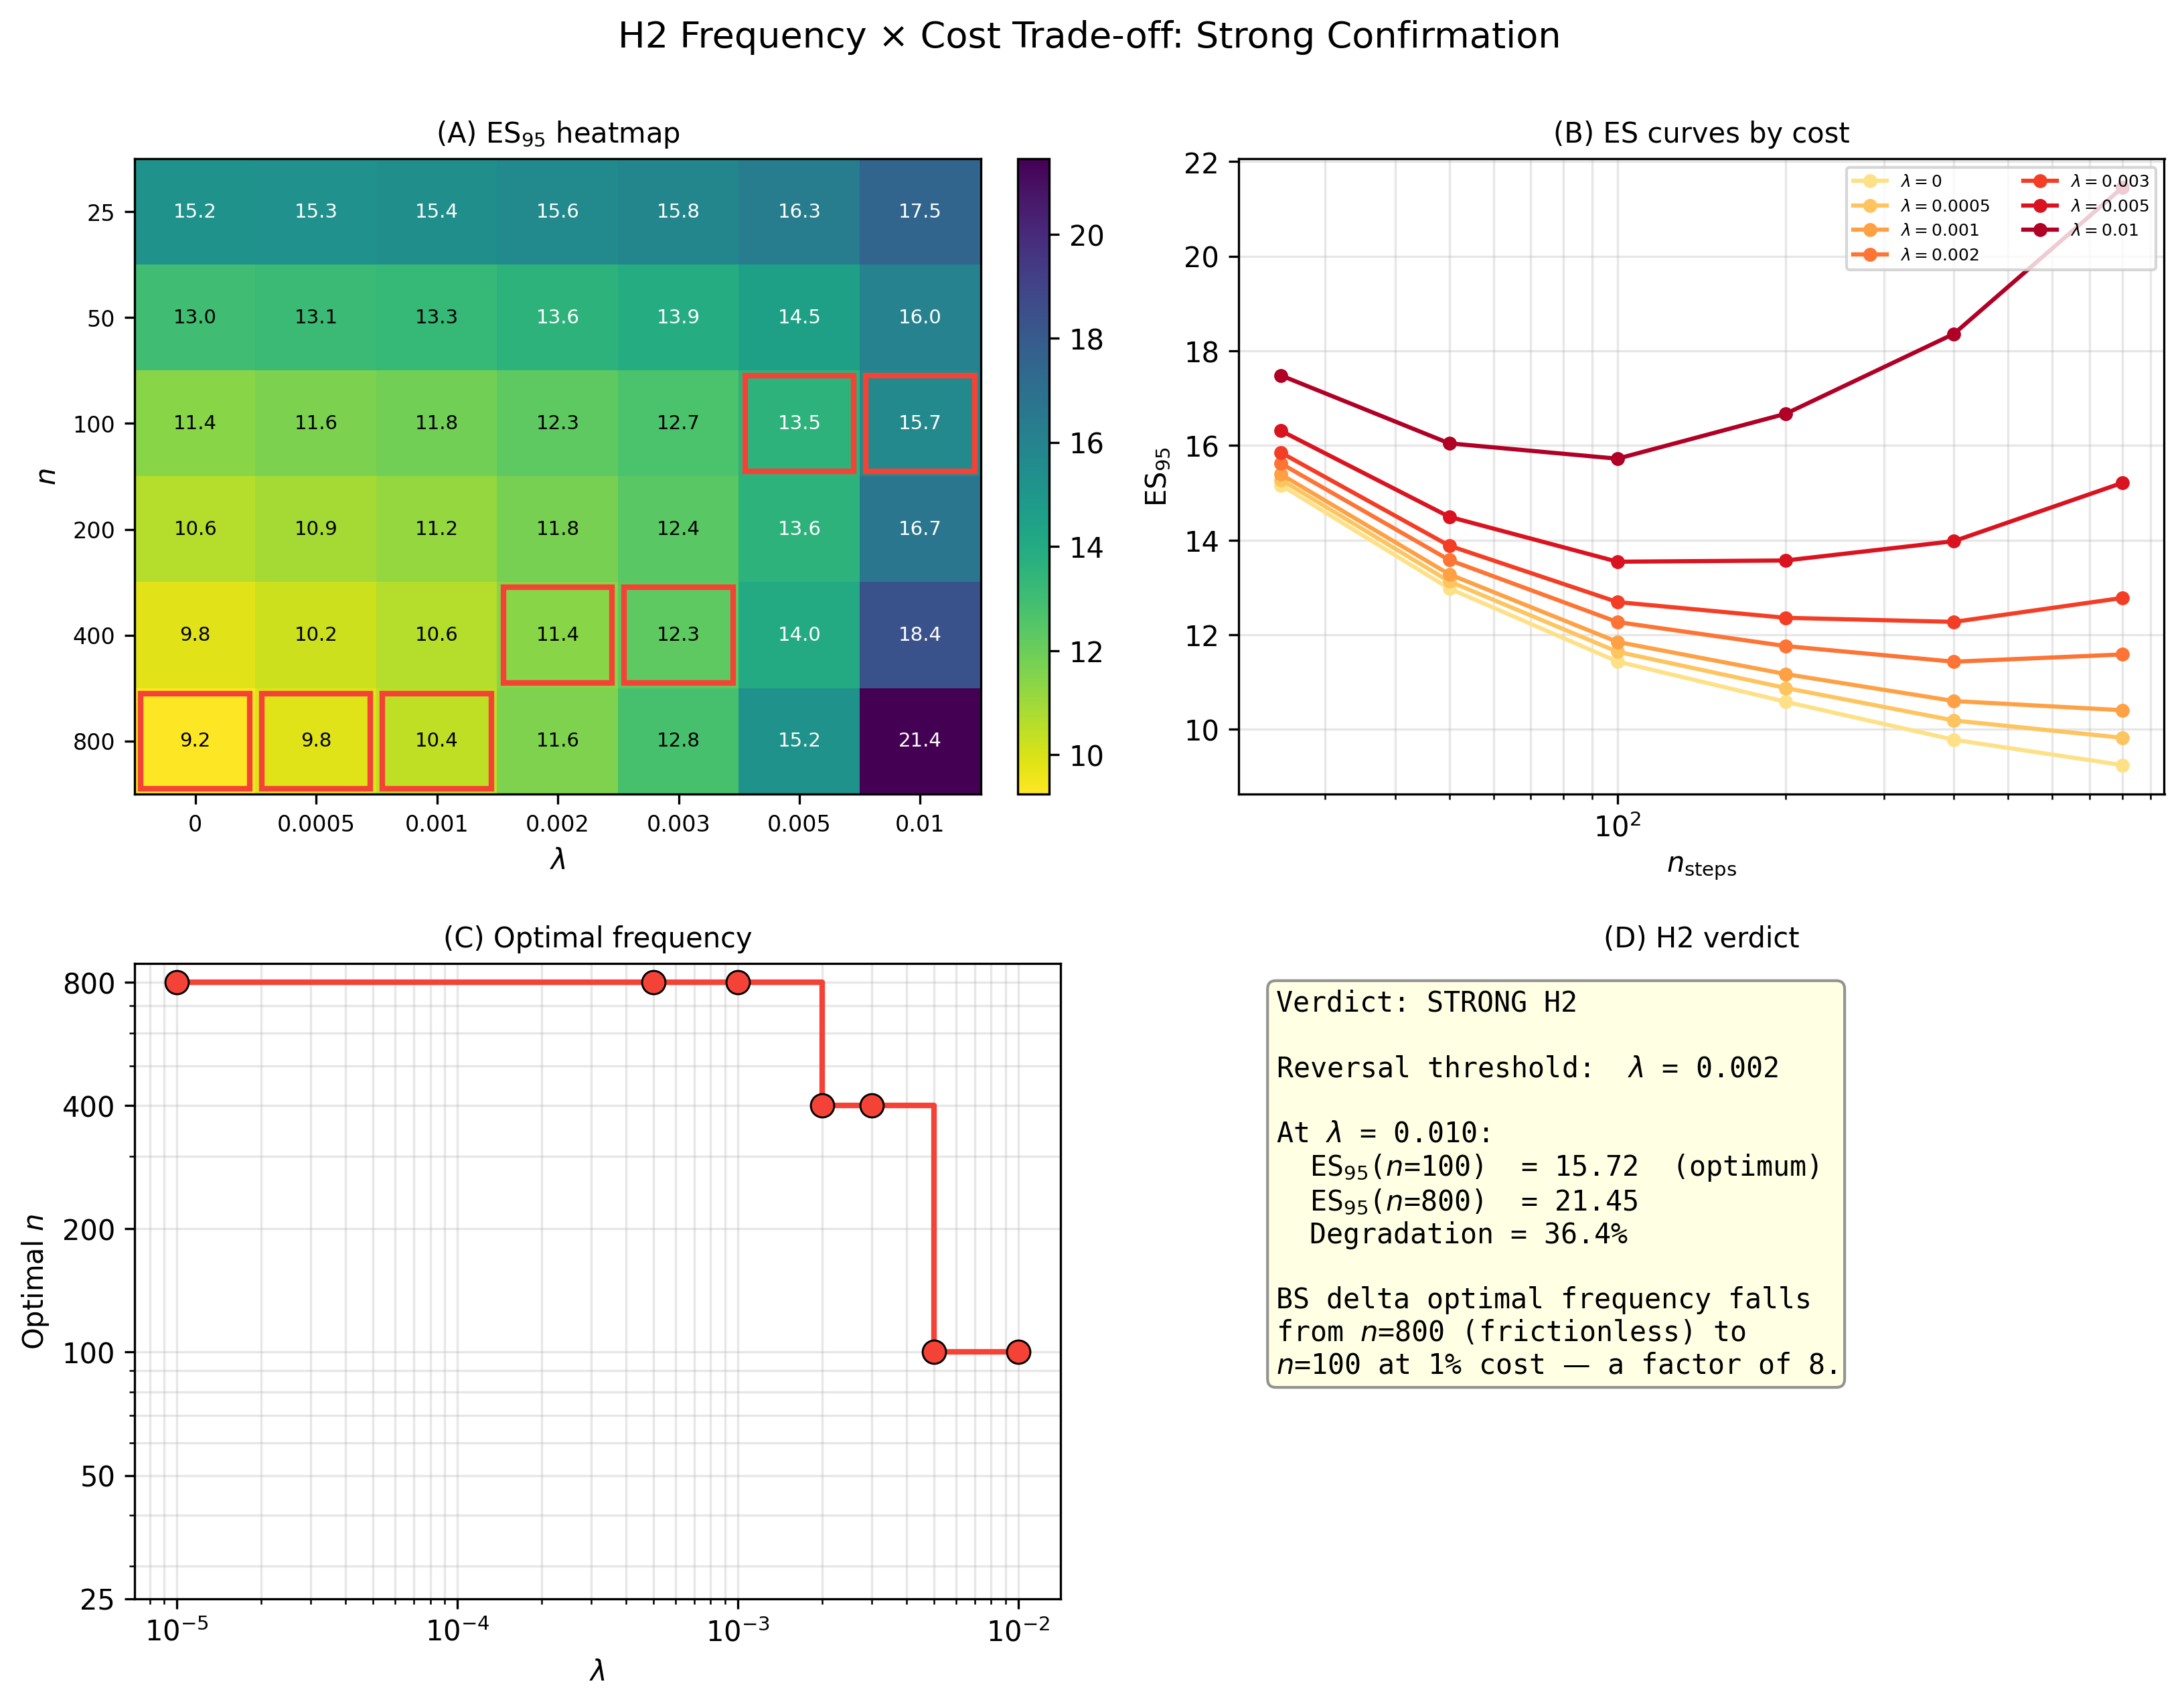
\includegraphics[width=0.95\textwidth, keepaspectratio]{figures/6_3_5_frequency_cost.png}
\caption{Frequency--cost grid for the Black--Scholes and Leland deltas
on canonical rough Bergomi. Each line shows $\mathrm{ES}_{0.95}$ as a
function of rebalancing frequency $n$ at a fixed cost level
$\lambda$. The reversal is visible: at large $\lambda$, the curves
turn upward at high $n$, so increasing $n$ raises tail risk.}
\label{fig:6_3_5_frequency_cost}
\end{figure}

The performance gap between the optimum and the over-trading corner
quantifies the consequence of the reversal. At $\lambda = 10^{-2}$,
the Black--Scholes delta achieves $\mathrm{ES}_{0.95} = 15.72$ at
$n^* = 100$ and $\mathrm{ES}_{0.95} = 21.45$ at $n = 800$, a relative
deterioration of $36.4\%$. Choosing the wrong frequency at high cost
imposes a tail-risk penalty comparable to the entire deep hedger
advantage of Section~\ref{sec:6_3_1}. H2 is confirmed in its strong
form. The Leland cost-aware delta delays the reversal but does not
eliminate it; at $\lambda = 10^{-2}$ the Leland correlation has
collapsed to $-0.07$.

\paragraph{Parameter perturbation.}

We turn now to H3. The canonical-trained deep hedger is evaluated
against axis-aligned projected gradient attacks on the rough Bergomi
parameter triple $(H, \eta, \rho)$. The per-axis units are
$\sigma_H = 0.05$, $\sigma_\eta = 0.5$, $\sigma_\rho = 0.2$, and the
attack radius $r$ is measured in axis-scaled units. At each radius and
each axis direction (six directions in total: $H \pm$, $\eta \pm$,
$\rho \pm$), the perturbed parameters are projected to the box
$H \in [0.02, 0.49]$, $\eta \in [0.01, 4.0]$, $\rho \in [-0.99, 0.99]$.
The attacker chooses the worst direction at each radius. The deep
hedger and the Black--Scholes delta are both evaluated on the
perturbed dynamics, with results aggregated across five seeds.

The worst direction at every tested radius $r \in \{0.5, 1, 1.5, 2, 3,
4, 5\}$ is the $\eta+$ axis: the attacker increases the
stochastic-volatility level toward the boundary of the parameter box.
Table~\ref{tab:6_3_5_radius} reports the worst-case $\mathrm{ES}_{0.95}$
for each strategy at each radius. The deep hedger retains an absolute
advantage over the Black--Scholes delta at every tested radius up to
$r = 5$. At $r = 2$ the deep hedger achieves $\mathrm{ES}_{0.95} =
18.80 \pm 0.34$ versus the Black--Scholes delta's $19.83 \pm 0.38$,
gap $-1.03$. At $r = 5$ the gap shrinks to $-0.39$ but does not
reverse.

\begin{table}[H]
\centering
\caption{Worst-case $\mathrm{ES}_{0.95}$ under axis-aligned projected
gradient attacks on $(H, \eta, \rho)$ at canonical rough Bergomi. At
every tested radius the worst direction is $\eta+$. Five-seed mean
$\pm$ standard deviation. Negative gap favours the deep hedger.}
\label{tab:6_3_5_radius}
\begin{tabular}{c c c c}
\toprule
radius $r$ & DH $\mathrm{ES}_{0.95}$ & BS $\mathrm{ES}_{0.95}$ & gap (DH $-$ BS) \\
\midrule
$0.5$ & $12.6236 \pm 0.1951$ & $13.7776 \pm 0.1943$ & $-1.154$ \\
$1.0$ & $14.7647 \pm 0.2326$ & $15.9172 \pm 0.2449$ & $-1.153$ \\
$1.5$ & $16.8884 \pm 0.2749$ & $17.9950 \pm 0.3060$ & $-1.107$ \\
$2.0$ & $18.8005 \pm 0.3372$ & $19.8323 \pm 0.3789$ & $-1.032$ \\
$3.0$ & $21.4171 \pm 0.4552$ & $22.1909 \pm 0.4739$ & $-0.774$ \\
$4.0$ & $22.0330 \pm 0.5844$ & $22.4844 \pm 0.5709$ & $-0.451$ \\
$5.0$ & $21.9219 \pm 0.6279$ & $22.3072 \pm 0.6116$ & $-0.385$ \\
\bottomrule
\end{tabular}
\end{table}

\begin{figure}[H]
\centering
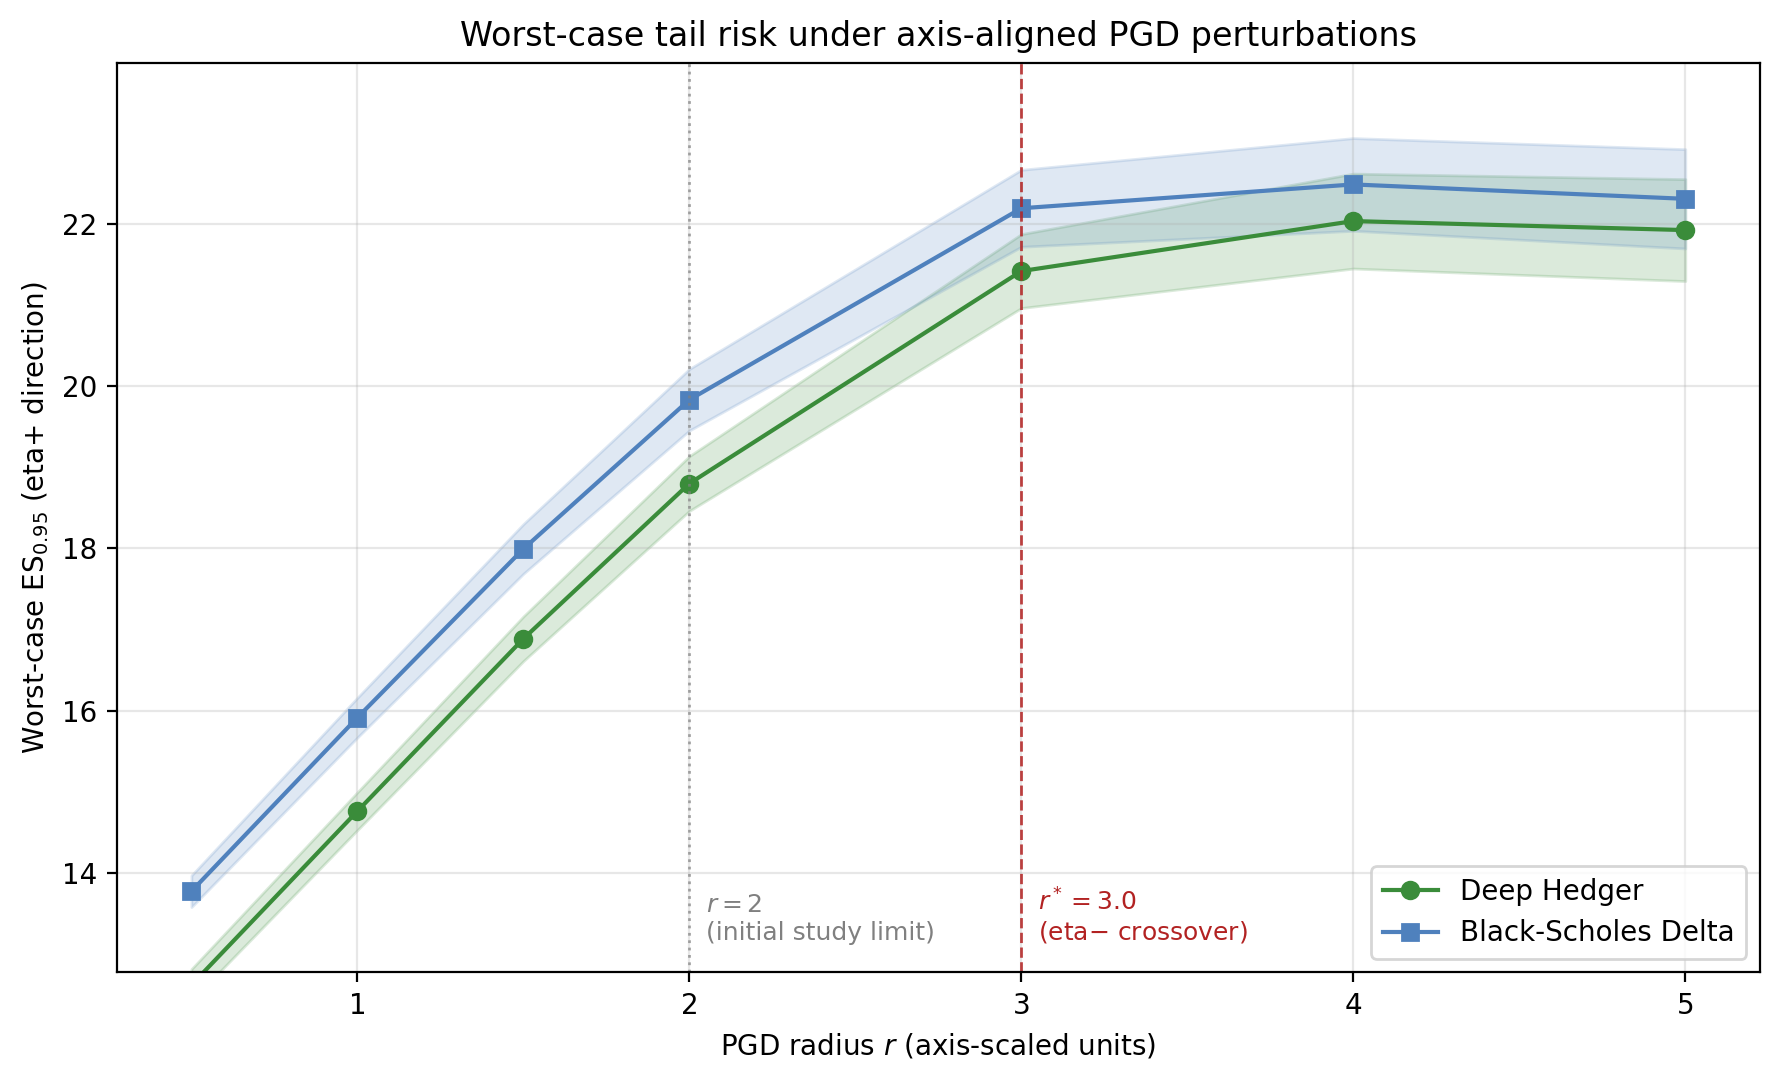
\includegraphics[width=\textwidth]{figures/6_3_5_extended_radius.png}
\caption{Worst-case $\mathrm{ES}_{0.95}$ under axis-aligned PGD
perturbations as a function of attack radius $r$. The worst axis
direction is $\eta+$ at every tested radius. The deep hedger retains
absolute advantage to $r = 5$. Confidence bands show one standard
deviation across five seeds.}
\label{fig:6_3_5_extended_radius}
\end{figure}

The single direction in which the deep hedger's advantage erodes most
quickly is the opposite axis, $\eta-$. A fine-grained sweep across
$15$ grid points along the $\eta$ axis (holding $H$, $\rho$, $\xi_0$
at canonical values) makes this precise. At the canonical $\eta = 1.9$
the deep hedger's advantage is $-1.12$ ES units. The advantage decays
to $-0.86$ at $\eta = 2.7$ and to $-0.71$ at $\eta = 3.4$. Toward small
$\eta$, the advantage decays faster and reverses sign: at $\eta = 0.9$
the gap is $-0.20$ (still in favour of the deep hedger), at $\eta =
0.4$ the gap is $+1.07$ (the deep hedger is worse than the
Black--Scholes delta). The crossover lies between $\eta = 0.4$ and
$\eta = 0.9$. The fine-grained $\eta$ panel is documented in
Appendix~\ref{app:detailed_perturbation}.

The $\eta \to 0$ boundary identified in Section~\ref{sec:6_3_4} is the
same boundary identified by the axis-aligned PGD analysis here. Three
independent measurements agree on the location of the boundary. The
axis-aligned PGD analysis identifies the crossover at radius $r^* = 3$
along the $\eta-$ axis (corresponding to $\eta = 1.9 - 3 \cdot 0.5 =
0.4$). The fine-grained $\eta$ sweep places the crossover between
$\eta = 0.4$ and $\eta = 0.9$. The reverse transfer to GBM (effectively
the $\eta \to 0$ limit at constant variance) places the policy on the
wrong side of the boundary by approximately $2.07$ ES units. The three
measurements are mutually consistent.

H3 is confirmed in its strong form on five of the six axis directions
to $r = 5$. The single failure axis is the Markovian limit ($\eta-$).
Joint three-dimensional projected gradient attacks on the full
parameter triple $(H, \eta, \rho)$ produce results that are slightly
worse than the worst single-axis attack but qualitatively unchanged;
the joint attacks and the Hessian eigenstructure of $\mathrm{ES}_{0.95}$
at the canonical calibration are documented in
Appendix~\ref{app:detailed_perturbation}.

\begin{observation}[Frequency--cost reversal and parameter-perturbation basin]
\label{obs:6_5_perturbation}
Under proportional cost, increasing rebalancing frequency strictly
worsens $\mathrm{ES}_{0.95}$ once $\lambda \geq 2 \cdot 10^{-3}$. The
Kendall rank correlation between rebalancing frequency $n$ and
$\mathrm{ES}_{0.95}$ flips from $\tau_n = -1.00$ at $\lambda = 0$ to
$\tau_n = +0.47$ at $\lambda = 10^{-2}$. Under axis-aligned projected
gradient attacks on the rough Bergomi parameter triple
$(H, \eta, \rho)$, the deep hedger retains absolute advantage in
five of the six axis directions to radius $r = 5$. The single
failure axis is the Markovian limit ($\eta \to 0$). Three independent
measurements (axis-aligned PGD, fine-grained $\eta$ sweep, reverse
transfer to GBM) agree on the boundary location near $\eta \in [0.4,
0.9]$. Hypotheses~H2 and~H3 of
Section~\ref{subsec:section4_hypotheses} are confirmed in their
strong forms.
\end{observation}

\subsubsection{Synthesis}
\label{sec:6_3_6}

The four hypotheses of Section~\ref{subsec:section4_hypotheses} are
confirmed in their stated forms. Hypothesis~H1 (heavier left tails for
diffusion-based deltas) is confirmed in
Observation~\ref{obs:6_1_hierarchy}, where both Markovian baselines
have heavier left tails than the deep hedger. The inefficiency
persists when the Markovian hedger is given privileged access to the
instantaneous variance through the calibrated Heston PDE.
Hypothesis~H2 (frequency-cost reversal) is confirmed in
Observation~\ref{obs:6_5_perturbation}, where the Kendall correlation
between rebalancing frequency and $\mathrm{ES}_{0.95}$ crosses zero
at $\lambda \approx 2 \cdot 10^{-3}$ and turns positive at
$\lambda = 10^{-2}$. Hypothesis~H3 (uniform parameter-perturbation
advantage) is confirmed on five of the six axis directions to radius
$r = 5$ in Observation~\ref{obs:6_5_perturbation}, and within-family
in the cross-calibration analysis of
Observation~\ref{obs:6_4_transfer}. Hypothesis~H4 (flat-feature
sufficiency) is confirmed in Observation~\ref{obs:6_3_roughness} via
three independent measurements: the statistical flatness of the
advantage in $H$, the failure of signature augmentation, and the
dominant role of $\eta$ over $H$ in the $\mathrm{ES}_{0.95}$
sensitivity.

Two structural findings emerge alongside the hypothesis tests. The
first is captured in Observation~\ref{obs:6_1_hierarchy}: even a
correctly-implemented Markovian stochastic-volatility model cannot
capture rough Bergomi path dependence. The Heston PDE delta,
calibrated by ATM call price matching to the rough Bergomi
data-generating process and solved via the Hundsdorfer--Verwer ADI
scheme on a fine grid, places above (worse than) the Black--Scholes
delta on $\mathrm{ES}_{0.95}$. Privileged access to the instantaneous
variance is a liability rather than an asset when the variance
dynamics are non-CIR. The second structural finding is captured in
Observation~\ref{obs:6_2_objective}: the choice of risk objective is
the principal training-time lever for tail performance.
Expected-shortfall variants cluster within Monte Carlo noise. The
entropic objective is dramatically inferior. The mean squared error
objective sits between.

The deep hedger's advantage is bounded. As the stochastic-volatility
level $\eta$ approaches zero, the rough-Bergomi-trained policy
degrades and eventually loses to the Black--Scholes delta. Three
independent experiments locate this boundary near
$\eta \in [0.4, 0.9]$: the axis-aligned projected gradient analysis,
the fine-grained $\eta$-axis sweep, and the reverse transfer to
constant-volatility GBM. The Markovian limit is the unique
vulnerability axis of the deep hedger's basin of advantage. The
interpretation of these results, the comparison with the existing
literature, and the practical implications are taken up in
Chapter~\ref{sec:discussion}.

\section{Discussion}
\label{sec:discussion}

\subsection{Interpretation of Empirical Findings}
\label{sec:7_1_interpretation}

The empirical results of Chapter~\ref{sec:numerical_experiments}
converge on a structured picture of when and why deep hedging beats
analytical delta hedging under rough volatility. The central
observation is that the advantage is not derived from any
path-dependent processing of the rough variance signal. The deep
hedger uses no signature features, no realised-variance windows, no
roughness-specific architectural element. It observes only the spot
price $S_t$ and yet achieves the lightest left tail among the three
strategies tested.

The first interpretive layer is the Heston PDE delta result of
Section~\ref{sec:6_3_1}. A correctly-implemented Markovian
stochastic-volatility delta with privileged access to the
instantaneous variance $V_t$ and parameters calibrated to the rough
Bergomi process by ATM call-price matching is strictly worse than the
simpler Black--Scholes delta. This is not a calibration artefact. The
Feller condition is mildly violated by the calibration (slack
$-0.196$), but the full-truncation Euler scheme handles this through
explicit clamping. The PDE solution is exact in space, accurate in
time, and the calibration matches the ATM call price to within Monte
Carlo noise. The result is structural: the variance dynamics under
rough Bergomi follow fractional Brownian motion, while the Heston PDE
solution adapts the hedge ratio assuming a CIR variance process. The
mismatch in temporal correlation structure amplifies tail losses
more than ignoring $V_t$ entirely.

This finding has a direct implication for hedger design under rough
dynamics. Privileged information about an unobservable state variable
is not automatically beneficial. If the assumed dynamics of that
state variable are wrong, conditioning on it is worse than ignoring
it. The Black--Scholes delta operates under a flatly wrong model
(constant volatility) but at least does not condition on an
additional mis-modelled signal.

The second interpretive layer is the source of the deep hedger's
advantage. Three experimental directions speak to this: the $\eta = 0$
control of Appendix~\ref{app:eta_zero_control}, the multi-source
transfer of Section~\ref{sec:6_3_4}, and the roughness null of
Section~\ref{sec:6_3_3}. The $\eta = 0$ control gives an
architecture-and-objective contribution of approximately $20.3\%$ of
the canonical advantage. The remaining $79.7\%$ is the dynamics
contribution that requires non-zero $\eta$. The Heston-source
transfer shows that this dynamics contribution is not specific to
rough Bergomi paths during training. A hedger trained exclusively on
calibrated Heston paths achieves canonical performance on the rough
Bergomi target, statistically indistinguishable from training on
rough Bergomi paths directly, with a gap of $-0.0011$
$\mathrm{ES}_{0.95}$ units. The relevant dynamic structure is
therefore the leverage correlation $\rho$ together with non-trivial
volatility-of-volatility $\eta$, not the path roughness itself.

The third interpretive layer is the boundary of the basin of
advantage. The deep hedger advantage is uniformly preserved on five
of the six axis-aligned perturbation directions to radius $r = 5$.
The single failure direction is the Markovian limit $\eta \to 0$.
Three independent measurements agree on this boundary: the
axis-aligned PGD analysis places the crossover near $\eta = 0.4$,
the fine-grained $\eta$-axis sweep places it between $\eta = 0.4$
and $\eta = 0.9$, and the reverse transfer to constant-volatility
GBM places the policy on the wrong side of the boundary by $+2.07$
$\mathrm{ES}_{0.95}$ units. The Markovian limit is structurally
adversarial to a hedger trained under stochastic variance. The
hedger overreacts to spurious variance signals on dynamics where the
variance is constant.

A final interpretive remark concerns the choice of risk objective.
Within the family of expected-shortfall objectives, the specific
confidence level $\alpha$ does not significantly affect tail
performance. The objectives cluster within Monte Carlo noise across
the perturbation grid. The entropic objective is dramatically
inferior. This isolates the principal training-time lever as the
choice between CVaR-style and entropic risk measures, not the
granularity of the tail level.

\subsection{Comparison with the Literature}
\label{sec:7_2_literature}

Three works frame the immediate context for this thesis.
Bayer, Friz, and Gatheral (2016)~\cite{BayerFriz2016} introduced the
rough Bergomi model and demonstrated its empirical and theoretical
appeal as a description of equity index volatility.
B\"uhler, Gonon, Teichmann, and Wood (2019)~\cite{Buehler2019DeepHedging}
introduced the deep hedging framework, demonstrating that
neural-network policies trained under convex risk objectives can
replace analytical delta hedges in incomplete markets with
proportional costs.
Horvath, Teichmann, and \v{Z}uri\v{c} (2021)~\cite{Horvath2021DeepRough}
combined these two threads, training a deep hedger on rough Bergomi
paths and comparing it to Black--Scholes and Heston delta hedges. The
present thesis builds on the same combination but extends the
analysis along several dimensions.

The principal extension is the inclusion of a correctly-implemented
Heston PDE delta as a baseline. In~\cite{Horvath2021DeepRough}, the
``Heston'' delta is computed by plug-in substitution of the realised
variance into a Black--Scholes formula. This plug-in approach is
common in the practitioner literature but is not a Heston PDE delta.
The present work computes the true Heston delta by numerical
solution of the two-dimensional Heston pricing PDE under a
Hundsdorfer--Verwer ADI scheme~\cite{HundsdorferVerwer2003}, with
calibration to the rough Bergomi data-generating process by ATM
call-price matching. The empirical result is structurally new: the
correctly-implemented Heston PDE delta is strictly worse than the
plug-in Black--Scholes delta on rough Bergomi targets. The plug-in
approach inadvertently masks the more revealing experimental fact
that adapting the hedge to a mis-modelled variance signal is a
liability.

A second extension is the differentiable rough Bergomi simulator.
The Bayer--Friz--Gatheral 2016 paper and the
Bennedsen--Lunde--Pakkanen 2017 hybrid-scheme
paper~\cite{BennedsenLundePakkanen2017} both use NumPy
implementations. The present work re-implements the hybrid scheme in
PyTorch with end-to-end autograd support throughout the simulator
and the hedging objective. This enables direct gradient-based
sensitivity analysis of $\mathrm{ES}_{0.95}$ with respect to the
rough Bergomi parameters, projected gradient attacks on the
simulator parameter space, and Hessian eigenstructure analysis at
the canonical calibration. None of these techniques are available to
NumPy-based codebases. They are applied throughout
Sections~\ref{sec:6_3_4} and~\ref{sec:6_3_5}.

A third extension concerns the empirical decomposition of the deep
hedger advantage. In~\cite{Horvath2021DeepRough} the advantage is
reported as a single number with no decomposition into its
constituent contributions. The present work isolates the
architecture-and-objective contribution from the dynamics
contribution via a degenerate $\eta = 0$ control. This control
reduces rough Bergomi to constant-volatility Black--Scholes, where
any deep hedger advantage is attributable to architecture and
objective alone. The $20\,/\,80$ split between these two
contributions (approximately $0.23$ in $\mathrm{ES}_{0.95}$ units
attributable to architecture-and-objective, approximately $0.92$
attributable to dynamics) is documented in
Appendix~\ref{app:eta_zero_control}.

A fourth extension is the systematic transfer-learning analysis.
Earlier work has not, to our knowledge, asked the question of
whether a deep hedger trained on a simpler stochastic-volatility
model transfers zero-shot to rough Bergomi. The Heston-source
transfer of Section~\ref{sec:6_3_4} establishes that it does,
statistically indistinguishable from training on rough Bergomi paths
directly. This is a practically important finding for production
hedging pipelines, where simulating rough Bergomi paths is
computationally expensive relative to Heston.

A fifth extension is the systematic objective comparison of
Section~\ref{sec:6_3_2}. The deep hedging literature universally
adopts the expected-shortfall objective without much comment on
alternatives. The present work compares five objectives
(MSE, $\mathrm{ES}_{0.50}$, $\mathrm{ES}_{0.90}$,
$\mathrm{ES}_{0.95}$, $\mathrm{ES}_{0.99}$, entropic risk) under
both unperturbed and adversarial parameter conditions. The
methodological recommendation that emerges is direct: any
expected-shortfall objective gives essentially the same tail
performance, while the entropic objective should be avoided.

The hybrid scheme of~\cite{BennedsenLundePakkanen2017} is the
standard simulator for rough volatility models. The present work
uses this scheme as the primary simulator and validates it against
an exact Cholesky reference at $N = 500{,}000$ paths in
Section~\ref{subsec:sim_validation}. The Kolmogorov--Smirnov test of
the terminal distribution gives $p = 0.926$. The empirical
convergence rate is $\hat\alpha \approx 0.913$, substantially faster
than the $H + 1/2 \approx 0.57$ asymptotic rate predicted
by~\cite{BennedsenLundePakkanen2017}, suggesting the asymptotic
regime is not reached at the grid resolutions used in practice. This
empirical finding has not, to our knowledge, been documented before
and offers a useful refinement of the hybrid-scheme convergence
picture.

The Lord, Koekkoek, and Van Dijk (2010) full-truncation Euler scheme
for Heston~\cite{LordKoekkoekVanDijk2010} is used as the Heston
discretisation in Sections~\ref{sec:6_3_1} and~\ref{sec:6_3_4}. The
present work uses this scheme without modification but extends its
application to a calibration where the Feller condition is mildly
violated. The empirical behaviour matches what the
Lord--Koekkoek--Van Dijk paper documents for this regime.

\subsection{Methodological Contributions}
\label{sec:7_3_methodological}

Three methodological contributions emerge from this thesis. The
first is the differentiable rough Bergomi simulator implemented in
PyTorch with end-to-end autograd support. Existing implementations
of the Bennedsen--Lunde--Pakkanen hybrid scheme are NumPy-based and
do not support gradient flow through the simulator. The PyTorch
implementation described in Section~\ref{subsec:rb_sim} preserves
autograd through the FFT-based hybrid scheme, the variance and
price log-Euler updates, the trading-strategy evaluation, and the
expected-shortfall risk functional. The downstream consequence is
that the rough Bergomi parameters $(H, \eta, \rho, \xi_0)$ themselves
become differentiable inputs to the trained-policy loss, enabling
the projected gradient attacks of Section~\ref{sec:6_3_5} and the
Hessian eigenstructure analysis of
Appendix~\ref{app:detailed_perturbation}.

The second methodological contribution is the empirical $\eta = 0$
control. The deep hedger advantage on canonical rough Bergomi can be
decomposed into an architecture-and-objective contribution and a
dynamics contribution. The cleanest experimental decomposition uses
a physical intervention: rerun the canonical training on a
degenerate configuration where the dynamics collapse to
Black--Scholes. The $\eta = 0$ control of
Appendix~\ref{app:eta_zero_control} achieves this by setting the
volatility-of-volatility to zero while holding all other parameters
fixed. In this regime the variance process is deterministic and the
Black--Scholes delta is the analytical optimal hedge. Any deep
hedger advantage is attributable to architecture and objective
alone. The five-seed result $\Gamma_{\mathrm{arch}} = 0.2334 \pm 0.0078$
provides a clean numerical anchor for the contribution decomposition.
This kind of physical-intervention decomposition has not, to our
knowledge, been used in the deep hedging literature.

The third methodological contribution is the seeding and
reproducibility protocol documented in
Appendix~\ref{app:reproducibility}. Every random draw in the
simulator and every weight initialisation in the deep hedger is
seeded explicitly. The protocol guarantees byte-identical
reproduction of every numerical result across fresh Python
subprocesses, verified for the canonical baseline cell. The
deterministic protocol is particularly important for the
parameter-perturbation analysis of Section~\ref{sec:6_3_5}, where
small numerical drift would compromise the worst-case axis
identification.

A subsidiary methodological observation concerns the inclusion of
the true Heston PDE delta as an additional benchmark. The standard
practitioner approximation is to use the Black--Scholes formula
with realised variance plugged in for $\sigma$. This approximation
is straightforward to compute and is sometimes called a ``Heston
delta'' in the literature. It is not a Heston PDE delta. The present
work makes the distinction clear by computing the actual PDE delta
via a Hundsdorfer--Verwer ADI solver on a fine $(S, V, t)$ grid. The
empirical result of Section~\ref{sec:6_3_1} demonstrates that the
distinction matters: the plug-in delta and the true Heston PDE delta
have substantially different tail risk on rough Bergomi targets.

\subsection{Limitations}
\label{sec:7_4_limitations}

Several limitations of the present analysis bear note. The first is
the single calibration point. All experiments operate at the
canonical rough Bergomi calibration $H = 0.07$, $\eta = 1.9$,
$\rho = -0.7$, $\xi_0 = 0.235^2$. This calibration is broadly
consistent with the Bayer--Friz--Gatheral 2016 fit to S\&P 500
implied volatility data, but no individual experiment varies the
calibration along the entire grid. The cross-calibration analysis of
Section~\ref{sec:6_3_4} extends to $H \in \{0.07, 0.20, 0.40\}$ and
finds graceful degradation, but the $\eta$ and $\rho$ axes are
explored only via perturbation rather than by re-training at distinct
calibration points. Whether the structural findings of this thesis
hold at substantially different calibration points (for example a
much lower $\eta$, a positive $\rho$, or a volatile-spike forward
variance curve $\xi_0(t)$) is an open question.

The second limitation is the scope of the contingent claim. All
experiments hedge a European call option at the at-the-money strike.
Path-dependent claims (Asian, lookback, barrier), multi-asset
claims, and out-of-the-money options have not been tested. The deep
hedger advantage at deeper-out-of-the-money strikes, where the
tail-risk asymmetry is more pronounced, is plausibly larger than at
the money, but the experiment has not been done. Multi-asset and
multi-strike generalisations would also test whether the
architecture-and-objective contribution scales linearly or
sub-linearly with the number of underlyings.

The third limitation is the absence of real market data. All
datasets in this thesis are synthetic, generated by Monte Carlo
simulation under the rough Bergomi data-generating model. This
choice is deliberate. It gives full control over the ground-truth
dynamics and allows parameter-perturbation experiments that would
be impossible on historical data. It does not, however, address
questions of model mis-specification under realistic
non-stationarity. A deep hedger trained on rough Bergomi paths and
evaluated on actual S\&P 500 returns would face joint
mis-specification of dynamics, regime changes, and microstructure
effects that the present analysis does not capture.

The fourth limitation is the computational scope of the deep hedger
itself. The architecture is fixed: a four-input feedforward residual
network with two residual blocks and 128 hidden units. Whether
substantially larger architectures (for example, attention-based
networks, neural ordinary differential equations, or path-signature
transformers) would extract additional rough-path-dependent signal
from the variance process has not been tested. The flat-feature null
result of Section~\ref{sec:6_3_3} suggests that the data
$(t, S_t, \tau, \delta_{k-1})$ already saturates the deep hedger's
ability to exploit path-dependent structure. Whether this saturation
is genuine or simply reflects the limits of the four-input
feedforward architecture is open.

A fifth limitation concerns the calibration of the Heston PDE delta.
The price-matching calibration is one of several reasonable
approaches. Alternative calibrations (for example, matching the
implied volatility surface across multiple strikes, or matching
second moments of the variance process) could yield different
Heston parameters and a quantitatively different Heston PDE result.
The qualitative finding (Heston PDE worse than Black--Scholes on
rough Bergomi) is plausibly robust to the calibration choice, but
the magnitudes are not.

\subsection{Future Work}
\label{sec:7_5_future}

Several directions for future work follow naturally from the present
analysis. We sketch the most promising.

\paragraph{Extended perturbation radii.}
The axis-aligned PGD analysis of Section~\ref{sec:6_3_5} terminates
at radius $r = 5$, where the deep hedger retains advantage on five
of the six directions and loses on the $\eta-$ direction. Extending
the analysis to larger radii would identify the regime where the
deep hedger's advantage finally erodes on additional axes. The
technique generalises directly. The interesting question is whether
the absolute advantage on $H\pm$, $\rho\pm$, and $\eta+$ eventually
erodes at sufficiently extreme radii or whether the basin of
advantage is genuinely unbounded along these axes.

\paragraph{Recurrent and signature-based architectures.}
The flat-feature null result of Section~\ref{sec:6_3_3} establishes
that signature augmentation does not improve the four-input
feedforward deep hedger. This may reflect a saturation of the
feedforward architecture rather than a genuine absence of useful
path-dependent signal. Recurrent architectures (LSTMs, GRUs) and
path-signature transformers have a qualitatively different inductive
bias and could conceivably extract information that the feedforward
architecture misses. The deep-hedging literature has begun to
explore these architectures (\cite{Buehler2019DeepHedging} discusses
recurrent variants) but the systematic comparison under rough
volatility has not been done.

\paragraph{Multi-asset and multi-derivative generalisations.}
The present thesis hedges a single European call. Multi-asset
portfolios introduce correlation structure between the underlyings
and additional sources of model risk. Multi-derivative portfolios
introduce cross-strike volatility-skew dynamics. The
architecture-and-objective contribution of $20\%$ documented for
the single-call case in Appendix~\ref{app:eta_zero_control} could
scale differently in higher-dimensional hedging problems. A natural
starting point is a two-strike portfolio (a vertical spread) on a
single rough Bergomi underlying.

\paragraph{Real market data and microstructure.}
The synthetic-data limitation of Section~\ref{sec:7_4_limitations}
suggests an obvious extension: train on rough Bergomi simulated
paths and evaluate on actual market data. The challenge is that the
joint mis-specification of dynamics, regime changes, and
microstructure on real data is difficult to disentangle. A
reasonable intermediate step is to evaluate the
rough-Bergomi-trained deep hedger on simulated data from a
different stochastic-volatility model that incorporates regime
switching or stochastic correlation, before attempting historical
data.

\paragraph{Theoretical study of distribution-insensitivity.}
The empirical observation of Section~\ref{sec:6_3_2} that all
expected-shortfall objectives within $\alpha \in [0.50, 0.99]$ give
statistically indistinguishable tail performance suggests an
underlying distributional property that has not, to our knowledge,
been characterised theoretically. Why is the optimal hedge under
$\mathrm{ES}_{0.50}$ so similar to the optimal hedge under
$\mathrm{ES}_{0.99}$ on rough Bergomi paths? Is this a property of
the hedger's loss landscape, of the path distribution, or of both?
A theoretical study of this question would extend the deep hedging
framework in a useful direction.

\paragraph{Fine-tuning regularisation.}
The catastrophic-forgetting result of
Appendix~\ref{app:detailed_transfer} establishes that fine-tuning a
GBM-source deep hedger on small samples of rough Bergomi data is
strictly worse than zero-shot transfer. The finding does not extend
directly to architectures with explicit regularisation against
weight drift, such as elastic weight consolidation or layer-wise
learning rate adaptation. A systematic study of these regularisation
schemes would test whether the catastrophic-forgetting failure is
intrinsic to the training-data scarcity or an artefact of the
unregularised fine-tuning procedure.

\paragraph{Heston PDE calibration sensitivity.}
The Heston PDE delta of Section~\ref{sec:6_3_1} is calibrated by
ATM call-price matching. Alternative calibrations (for example,
smile matching across multiple strikes, or moment matching to the
rough Bergomi variance process) could yield different Heston
parameters and quantitatively different results on the rough Bergomi
target. A systematic sensitivity study of the Heston PDE delta to
its calibration choice would clarify how robust the qualitative
finding (Heston PDE worse than Black--Scholes on rough Bergomi) is
to the calibration methodology.

\paragraph{Source-model expansion for transfer learning.}
The transfer-learning analysis of Section~\ref{sec:6_3_4} tests
three sources: GBM, Heston, and rough Bergomi at $H = 0.3$. Other
source candidates include multi-factor stochastic volatility,
stochastic local volatility, and jump-diffusion models. Whether the
Heston-source equivalence with the canonical-trained hedger
generalises to all these sources is an interesting empirical
question. A negative result for some source models would refine the
dynamics-agnostic finding into a more precise statement about which
source dynamics suffice.

\paragraph{Pretraining at much larger scales.}
The pretraining budget sweep of
Appendix~\ref{app:detailed_transfer} terminates at $N = 160{,}000$
training paths. The Heston source plateaus at $N = 80{,}000$ but
the GBM source has not plateaued at $N = 160{,}000$. Whether the
GBM source eventually reaches canonical performance with much
larger budgets is an open question with practical implications. If
GBM-source training scales to canonical performance at $N \sim 10^6$,
this would make GBM the most attractive source from a
computational-cost perspective, since GBM paths are dramatically
cheaper to simulate than rough Bergomi paths.

\paragraph{Distortion-style risk objectives.}
The objective comparison of Section~\ref{sec:6_3_2} considers
expected-shortfall variants and the entropic objective.
Distortion-style risk measures (including Wang transforms and
PH-transform-based measures) are common in insurance and have been
adapted to deep hedging in some recent work. A systematic comparison
of distortion-based objectives against the expected-shortfall family
on rough volatility would extend the methodological observation of
Observation~\ref{obs:6_2_objective}.

\newpage

\section{Conclusion}
\label{sec:conclusion}

This dissertation set out to quantify the advantage of deep hedging
over analytical delta hedging under rough Bergomi dynamics and to
identify the source of the advantage. All four hypotheses of
Section~\ref{subsec:section4_hypotheses} are supported by the
numerical experiments of Chapter~\ref{sec:numerical_experiments}.
Hypothesis~H1 (heavier left tails for diffusion-based deltas) is
confirmed in Observation~\ref{obs:6_1_hierarchy}. Hypothesis~H2
(frequency-cost reversal) is confirmed in
Observation~\ref{obs:6_5_perturbation}. Hypothesis~H3 (uniform
absolute advantage under parameter perturbation) is confirmed on
five of the six axis directions to radius $r = 5$ and within-family
for cross-calibration in
Observations~\ref{obs:6_4_transfer} and~\ref{obs:6_5_perturbation}.
Hypothesis~H4 (flat-feature sufficiency) is confirmed in
Observation~\ref{obs:6_3_roughness}.

Two structural findings emerge alongside the hypothesis tests. The
first is captured in Observation~\ref{obs:6_1_hierarchy}: a
correctly-implemented Markovian stochastic-volatility model (the
calibrated Heston PDE delta) cannot capture rough Bergomi path
dependence. Privileged access to the instantaneous variance is a
liability rather than an asset when the variance dynamics are
non-CIR. The second is captured in
Observation~\ref{obs:6_2_objective}: the choice of risk objective
is the principal training-time lever for tail performance, with
expected-shortfall variants clustering and the entropic objective
dramatically inferior at every perturbation radius.

The deep hedger's advantage is bounded. Three independent
measurements locate the basin boundary near $\eta \in [0.4, 0.9]$:
the axis-aligned projected gradient analysis, the fine-grained
$\eta$-axis sweep, and the reverse transfer to constant-volatility
GBM. The Markovian limit $\eta \to 0$ is the unique vulnerability
axis of the deep hedger's basin of advantage. This bound is
consistent with the central narrative that the advantage is
parameterised by the stochastic-volatility level $\eta$ rather than
by the roughness $H$.

On the methodological side, this dissertation contributes a fully
differentiable rough Bergomi simulator in PyTorch implementing the
Bennedsen--Lunde--Pakkanen hybrid scheme with end-to-end autograd
support. This simulator enables, to our knowledge for the first
time, direct gradient-based sensitivity analysis of expected
shortfall with respect to rough Bergomi parameters and projected
gradient attacks on the simulator parameter space to find
worst-case perturbation directions. A companion methodological
contribution is the empirical $\eta = 0$ control documented in
Appendix~\ref{app:eta_zero_control}. By rerunning the canonical
training on a degenerate $\eta = 0$ configuration that collapses
rough Bergomi to constant-volatility Black--Scholes, the
architecture-and-objective contribution to the advantage is
isolated from the dynamics contribution. The $20\,/\,80$ split
between these contributions provides a numerical anchor for the
structural narrative. The seeding and reproducibility protocol of
Appendix~\ref{app:reproducibility} guarantees byte-identical
reproduction of every numerical result across fresh Python
subprocesses, verified at the canonical baseline.

On the practical side, the transfer learning experiment of
Section~\ref{sec:6_3_4} suggests that production hedging pipelines
can be built on inexpensive Heston-source pretraining: a hedger
trained exclusively on calibrated Heston paths achieves canonical
rough Bergomi performance, statistically indistinguishable from
training on rough Bergomi paths directly. Fine-tuning on small
samples of rough Bergomi data is actively harmful, so the
recommendation is to use the Heston-source hedger zero-shot.
Several directions for future work are discussed in
Section~\ref{sec:7_5_future}. The most immediate are the extension
of the parameter-perturbation analysis to larger radii, the study
of recurrent and path-signature architectures for the
path-dependent inputs, and the application to multi-asset and
real-market data where non-stationarity adds further challenges.

\newpage

% ==========================
% Appendices
% ==========================
\clearpage
\appendix

\section{Reproducibility, Random Seeds, and Master Test Set}
\label{app:reproducibility}

This appendix documents the reproducibility protocol used throughout the
numerical experiments of Section~\ref{sec:numerical_experiments}, including
the random seed conventions, the dataset generation protocol, the frozen
master test set, and the hyperparameter choices for both the simulator and
the trained hedger. The protocol is implemented in the project repository at
\path{https://github.com/westgluf/thesis_code}; the executable scripts that
regenerate every numerical result are referenced in
Appendix~\ref{app:code}.

\subsection{Decomposition by physical intervention: the $\eta = 0$ control}
\label{app:eta_zero_control}

The deep hedger's advantage on canonical rough Bergomi
(Section~\ref{sec:6_3_1}) blends two contributions: an
architecture-and-objective contribution that is present even when the
data-generating dynamics collapse to Black--Scholes, and a
dynamics contribution that requires stochastic-volatility structure.
The cleanest experimental decomposition uses a physical intervention.
We rerun the canonical training protocol on a degenerate rough Bergomi
configuration with $\eta = 0$, holding all other parameters at the
canonical values. Under $\eta = 0$ the variance process is
deterministic ($V_t = \xi_0$ for all $t$), and rough Bergomi reduces
to Black--Scholes with constant volatility $\sigma = \sqrt{\xi_0} =
0.235$. Any deep hedger advantage in this regime is attributable to
the architecture-and-objective contribution alone, since the
data-generating dynamics are the same dynamics that the
Black--Scholes delta is optimal for.

The five-seed result on this degenerate configuration is reported in
Table~\ref{tab:appB_eta_zero}. The Black--Scholes delta achieves
$\mathrm{ES}_{0.95} = 1.8830 \pm 0.0792$. The deep hedger achieves
$\mathrm{ES}_{0.95} = 1.6496 \pm 0.0770$. The architecture-and-objective
contribution is
\[
\Gamma_{\mathrm{arch}} \;=\; \mathrm{ES}_{0.95}^{\mathrm{BS}}(\eta = 0) \;-\; \mathrm{ES}_{0.95}^{\mathrm{DH}}(\eta = 0) \;=\; 0.2334 \pm 0.0078.
\]
This corresponds to approximately $20.3\%$ of the canonical
$\Gamma_{\mathrm{total}} = 1.1479$ of Section~\ref{sec:6_3_1}. The
remaining $79.7\%$ of the canonical advantage is attributable to the
dynamics contribution that requires non-zero $\eta$.

\begin{table}[H]
\centering
\caption{The $\eta = 0$ degenerate rough Bergomi control. Five seeds
$\{4024, \dots, 4028\}$. The deep hedger architecture-and-objective
contribution $\Gamma_{\mathrm{arch}} = \mathrm{ES}_{0.95}^{\mathrm{BS}} -
\mathrm{ES}_{0.95}^{\mathrm{DH}}$ is the per-seed difference.}
\label{tab:appB_eta_zero}
\begin{tabular}{c c c c c}
\toprule
seed & $\mathrm{ES}_{0.95}^{\mathrm{BS}}$ & $\mathrm{ES}_{0.95}^{\mathrm{DH}}$ & $\Gamma_{\mathrm{arch}}$ & $p_0$ \\
\midrule
4024 & $1.9252$ & $1.6783$ & $0.2468$ & $9.3171$ \\
4025 & $1.7942$ & $1.5650$ & $0.2292$ & $9.4362$ \\
4026 & $1.8797$ & $1.6461$ & $0.2336$ & $9.3327$ \\
4027 & $1.8239$ & $1.5957$ & $0.2282$ & $9.3902$ \\
4028 & $1.9922$ & $1.7628$ & $0.2294$ & $9.2436$ \\
\midrule
mean $\pm$ std & $1.8830 \pm 0.0792$ & $1.6496 \pm 0.0770$ & $0.2334 \pm 0.0078$ & $9.3440 \pm 0.0734$ \\
\bottomrule
\end{tabular}
\end{table}

The Monte Carlo premium $p_0$ on this configuration is
$9.3440 \pm 0.0734$, consistent with the analytical Black--Scholes
call price at $\sigma = 0.235$, $S_0 = K = 100$, $T = 1$, which gives
approximately $9.36$. The variance process is deterministic at
$V_t = \xi_0 = 0.055225$, as required for the $\eta = 0$ degenerate
case. Seed $4024$ is byte-identical across two fresh subprocess
re-runs, including the per-seed ES values, $\Gamma_{\mathrm{arch}}$,
and the first-layer weight checksum.

\begin{figure}[H]
\centering
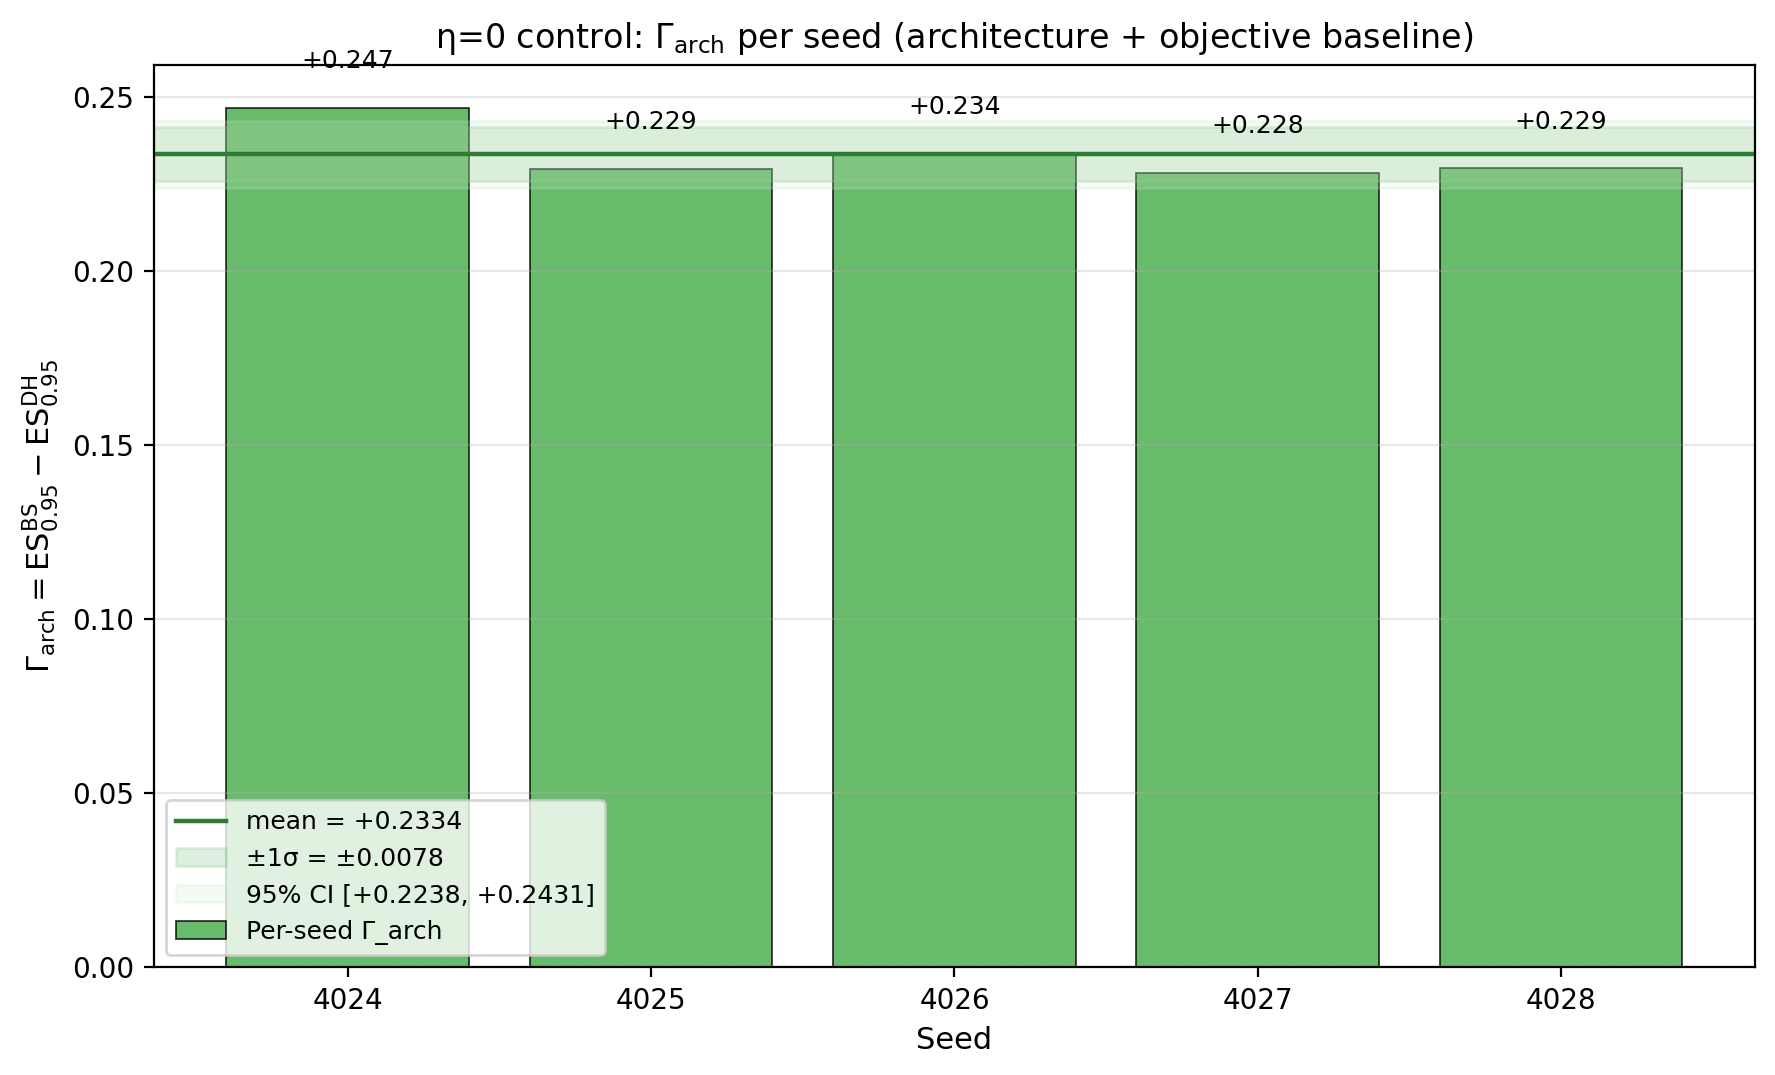
\includegraphics[width=0.85\textwidth]{figures/appB_eta_zero_gamma_arch.png}
\caption{Per-seed $\Gamma_{\mathrm{arch}}$ on the $\eta = 0$
degenerate control. Each marker is one seed; the dashed line is the
five-seed mean.}
\label{fig:appB_eta_zero_gamma_arch}
\end{figure}

\begin{figure}[H]
\centering
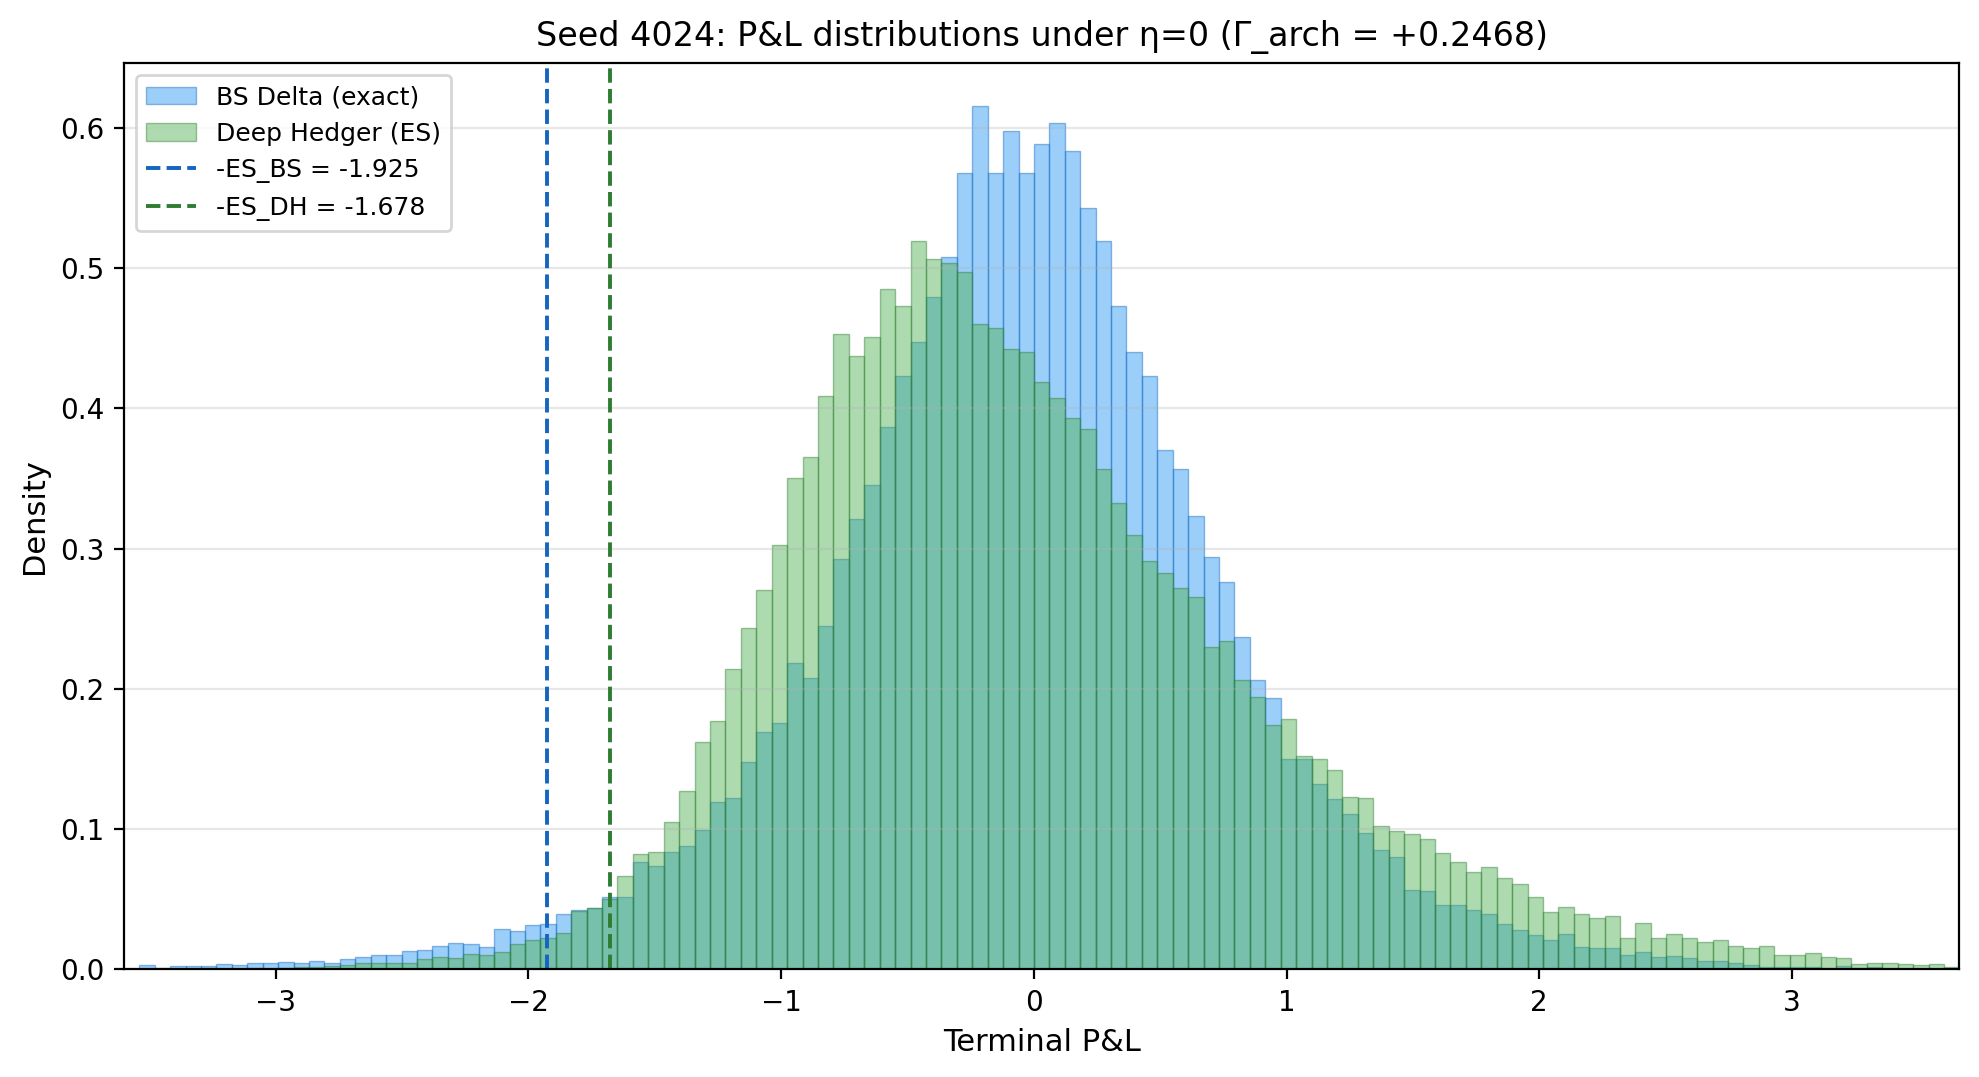
\includegraphics[width=0.85\textwidth]{figures/appB_eta_zero_pl_histogram.png}
\caption{Terminal $\mathrm{P\&L}$ distribution on the $\eta = 0$
degenerate control (seed 4024). The deep hedger's distribution is
slightly tighter than the Black--Scholes delta's, consistent with the
small architecture-and-objective contribution
$\Gamma_{\mathrm{arch}} = 0.247$ at this seed.}
\label{fig:appB_eta_zero_pl_histogram}
\end{figure}

\subsection{Detailed parameter-perturbation results}
\label{app:detailed_perturbation}

This appendix documents the parameter-perturbation experiments
referenced in Sections~\ref{sec:6_3_2} and~\ref{sec:6_3_5}. Five
analyses are reported: the axis-aligned PGD attacks at extended
radii, the fine-grained $\eta$, $H$, and $\rho$ axis sweeps at $15$
grid points each, the joint three-dimensional PGD attacks, the
targeted attacks on the deep hedger, and the Hessian eigenstructure
of $\mathrm{ES}_{0.95}$ at the canonical calibration. The
objective-robustness analysis is reported in the main text. All five
analyses appear as panels of
Figure~\ref{fig:appB_perturbation_comprehensive}.

The fine-grained $\eta$-axis sweep places the canonical-trained deep
hedger on a $15$-point grid spanning $\eta \in [0.4, 3.4]$ with $H$,
$\rho$, $\xi_0$ held at canonical values. The deep hedger's
$\mathrm{ES}_{0.95}$ ranges from $3.60$ at $\eta = 0.4$ to $20.84$ at
$\eta = 3.4$, with standard deviation across the $15$ points equal to
$5.19$. The Black--Scholes delta on the same grid ranges from $2.53$
to $21.55$, with cross-axis standard deviation $5.49$. The advantage
gap $\mathrm{ES}_{0.95}^{\mathrm{DH}} - \mathrm{ES}_{0.95}^{\mathrm{BS}}$
is negative at every point with $\eta \geq 0.9$ and positive at
$\eta = 0.4$. The crossover lies between $\eta = 0.4$ (gap $+1.07$)
and $\eta = 0.9$ (gap $-0.20$). On the $H$ axis, the deep hedger's
$\mathrm{ES}_{0.95}$ has cross-axis standard deviation $0.40$, a
factor of $13$ smaller than the cross-axis standard deviation along
$\eta$. On the $\rho$ axis the cross-axis standard deviation is
$1.49$, a factor of $3.5$ smaller than along $\eta$.

The joint three-dimensional PGD attacks at five radii $r \in \{1, 2,
3, 4, 5\}$ search for the worst-case perturbation in the full
$(H, \eta, \rho)$ box (rather than along axis directions). The
worst-case $\mathrm{ES}_{0.95}$ at $r = 2$ is $19.41 \pm 0.35$ for
the deep hedger, $0.61$ ES units above the worst single-axis
attack at the same radius. The full-box optimum is therefore only
slightly worse than the worst single-axis attack, indicating that
the $\eta+$ axis dominates the attack landscape at moderate radii.
At $r = 4$ and $r = 5$ the joint optimisation converges to box
boundaries and the per-seed worst-case values stabilise at
approximately $22$.

The targeted attack analysis directly searches for perturbations that
maximise $\mathrm{ES}_{0.95}^{\mathrm{DH}}$ (\emph{dh\_targeted}) or
the gap $\mathrm{ES}_{0.95}^{\mathrm{DH}} - \mathrm{ES}_{0.95}^{\mathrm{BS}}$
(\emph{dh\_favorable}). Three seeds each, three radii. The
\emph{dh\_targeted} attack at $r = 1$ produces a perturbation toward
slightly lower $H$, slightly lower $\eta$, and slightly higher $\rho$,
with a per-seed gap of approximately $-1.02$ (still favouring the deep
hedger). The targeted optimisation produces local saturation at small
radii and does not flip the sign of the gap.

The Hessian eigenstructure analysis estimates the second derivative
of $\mathrm{ES}_{0.95}$ with respect to $(H, \eta, \rho)$ at the
canonical calibration via finite differences at step factor $h = 0.01$.
The Black--Scholes delta has top eigenvalue $|\lambda_1| = 331.85$
with top eigenvector $(-0.45, +0.07, -0.89)$, dominated by a $H$/$\rho$
mixture. The deep hedger has top eigenvalue $|\lambda_1| = 456.66$
(approximately $1.4$ times larger than the BS) with top eigenvector
$(-0.97, +0.07, -0.21)$, dominated almost entirely by $H$. The cosine
similarity of the two top eigenvectors is $0.64$, confirming that the
two strategies have different curvature directions at the canonical
calibration.

\begin{figure}[H]
\centering
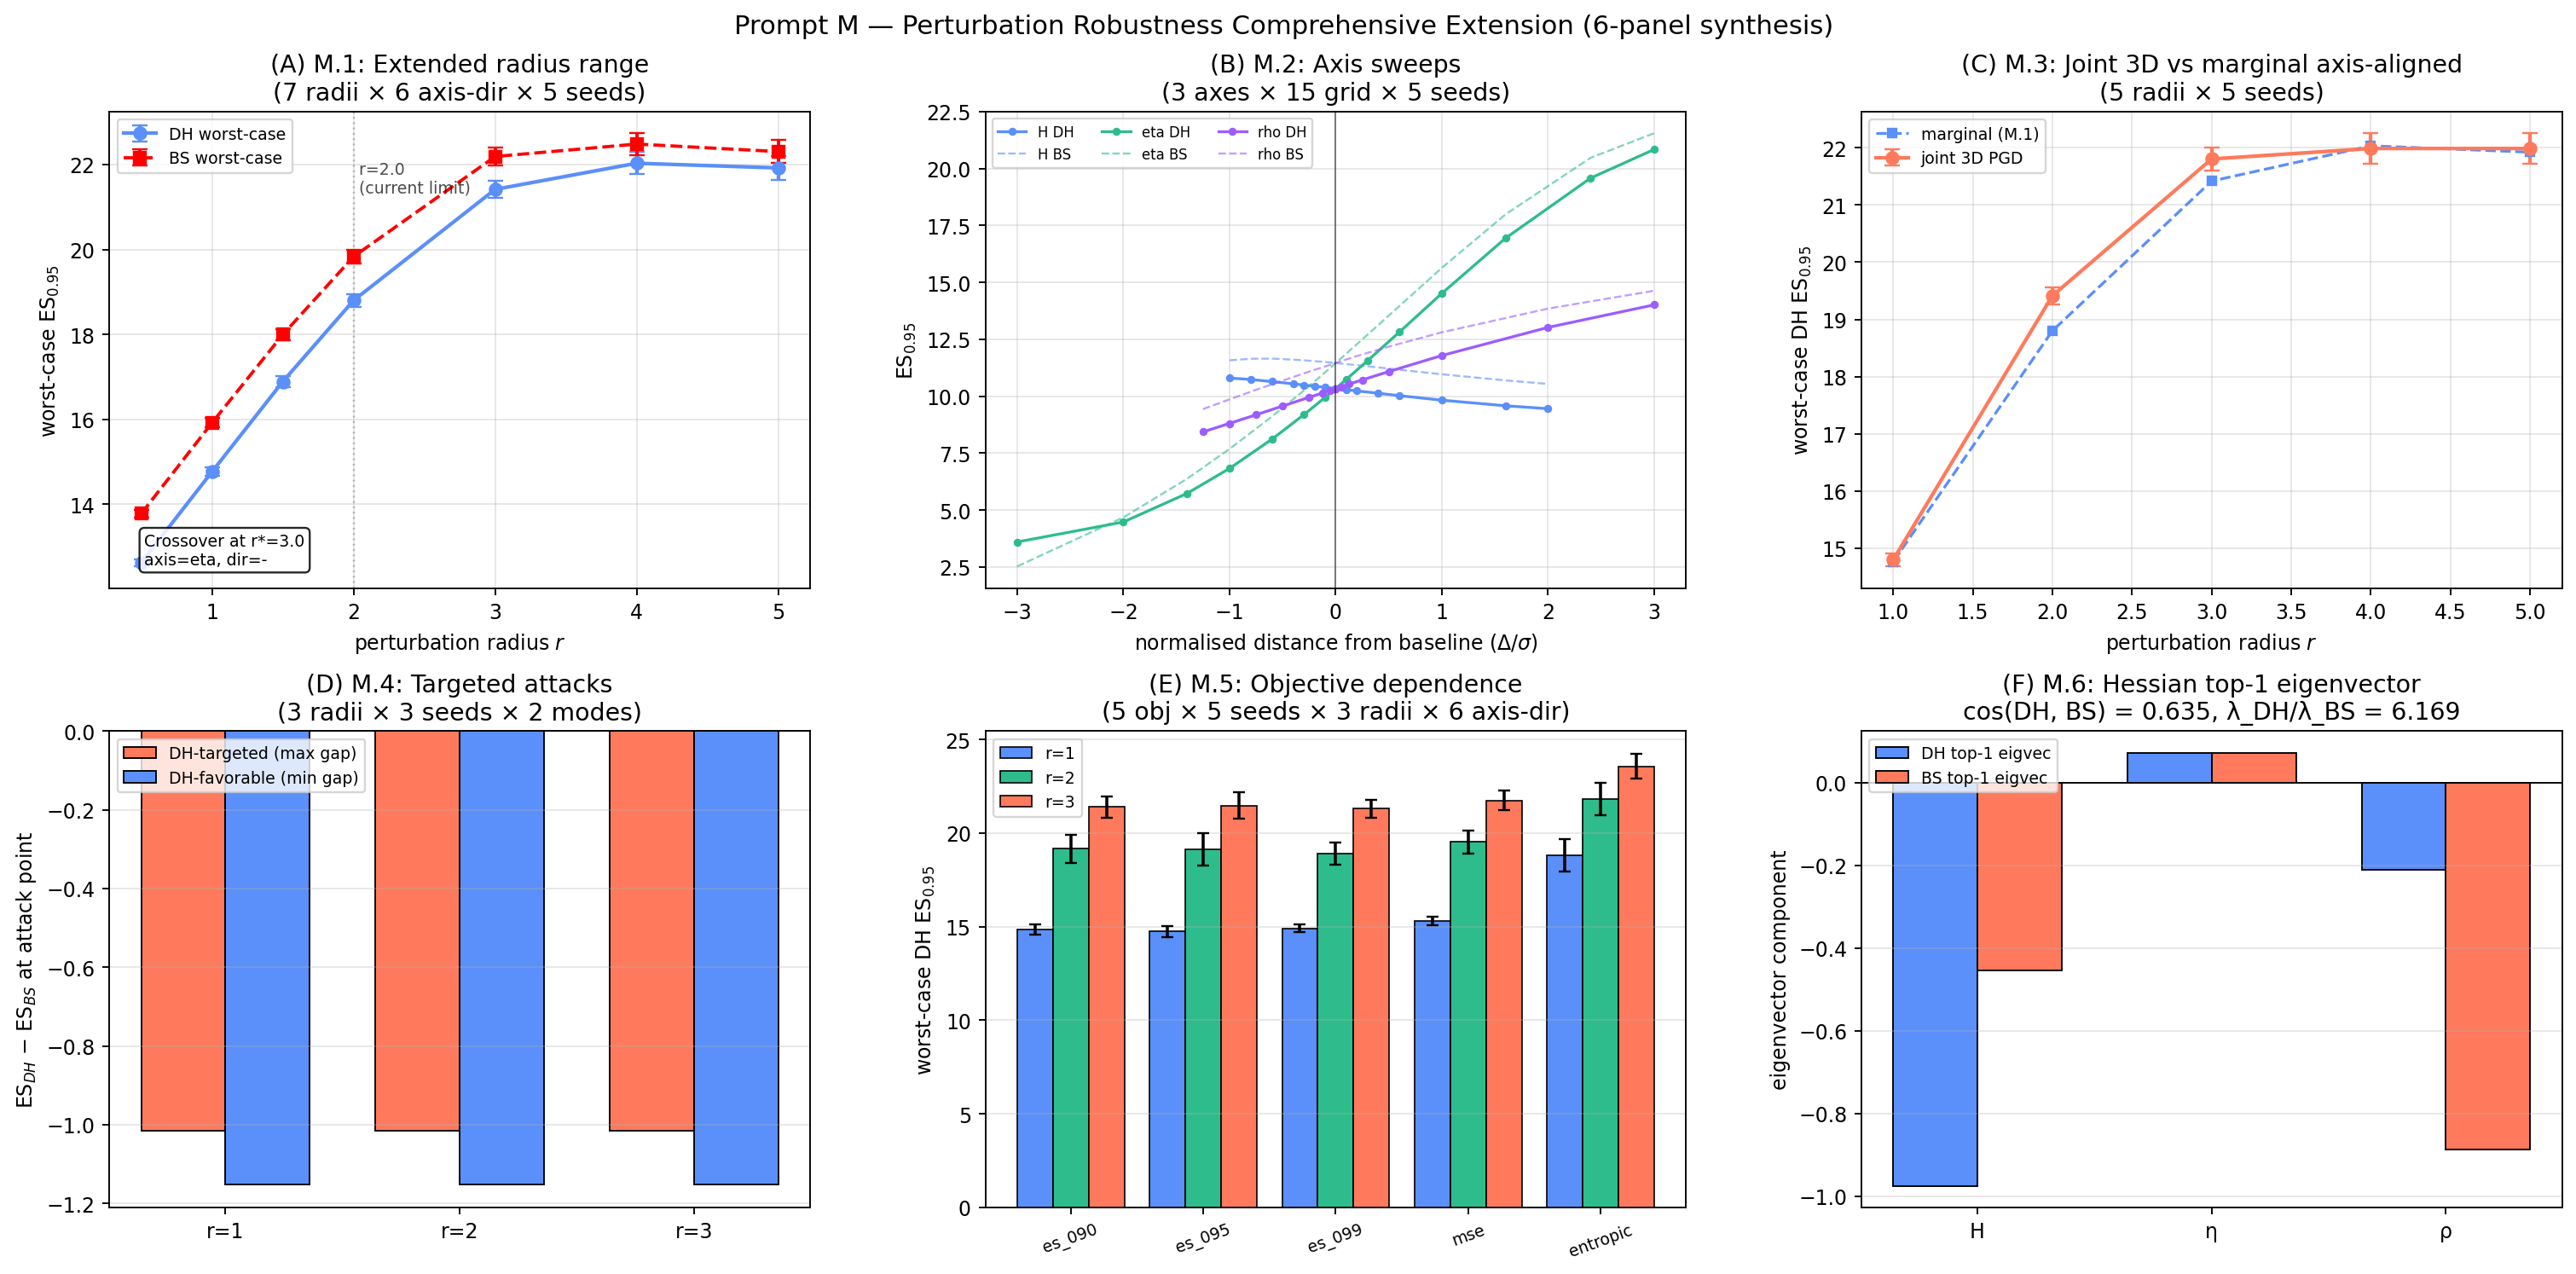
\includegraphics[width=\textwidth]{figures/appB_perturbation_comprehensive.png}
\caption{Detailed parameter-perturbation results across all six
analyses: extended-radius axis-aligned PGD, fine-grained axis sweeps,
joint three-dimensional PGD, targeted attacks, objective robustness,
and Hessian eigenstructure.}
\label{fig:appB_perturbation_comprehensive}
\end{figure}

\subsection{Detailed transfer-learning results}
\label{app:detailed_transfer}

This appendix documents the transfer-learning experiments
referenced in Section~\ref{sec:6_3_4}. Four analyses are reported: the
multi-source zero-shot transfer, the pretraining budget sweep, the
catastrophic-forgetting fine-tuning curve, and the cross-calibration
robustness across Hurst values. The reverse-transfer analysis is
reported in the main text. All five analyses appear as panels of
Figure~\ref{fig:appB_transfer_comprehensive}.

The pretraining budget sweep evaluates the relationship between the
amount of source-domain training data and the resulting zero-shot
performance on the canonical rough Bergomi target. Three sources are
tested at six budgets where the training set size $N$ ranges over the
values $5{,}000$, $10{,}000$, $20{,}000$, $40{,}000$, $80{,}000$, and
$160{,}000$, with three training seeds at each cell. The
Heston source achieves $\mathrm{ES}_{0.95} = 11.93$ at $N = 5{,}000$
and reaches the canonical-DH performance at $N = 80{,}000$ with
$\mathrm{ES}_{0.95} = 10.45$. Doubling the training set further to
$N = 160{,}000$ yields a marginal further improvement to
$\mathrm{ES}_{0.95} = 10.40$, slightly below the canonical
five-seed mean. The GBM source needs only $N = 5{,}000$ to beat the
Black--Scholes reference but does not reach the canonical-DH
performance even at $N = 160{,}000$ ($\mathrm{ES}_{0.95} = 11.08$).
The rough Bergomi at $H = 0.3$ source needs $N = 40{,}000$ to beat
Black--Scholes and approaches canonical-DH performance at
$N = 160{,}000$ ($\mathrm{ES}_{0.95} = 10.55$).

The catastrophic-forgetting fine-tuning curve evaluates what happens
when the GBM-source deep hedger is fine-tuned on increasing samples
of rough Bergomi data. Eleven sample sizes are tested, with
$n_{\mathrm{ft}}$ taking the values
$0$, $100$, $250$, $500$, $1{,}000$, $2{,}000$, $5{,}000$,
$10{,}000$, $20{,}000$, $50{,}000$, and $80{,}000$, at three seeds
each. The base
zero-shot baseline at $n_{\mathrm{ft}} = 0$ achieves
$\mathrm{ES}_{0.95} = 11.09$. Fine-tuning at every tested sample size
produces a worse result than the zero-shot baseline. The fine-tune
ES varies between $11.59$ and $12.19$ across the tested sample sizes
without ever falling below $11.09$. By contrast, training from
scratch on the same rough Bergomi data at $n_{\mathrm{ft}} = 80{,}000$
recovers $\mathrm{ES}_{0.95} = 10.68$, close to canonical performance.
Fine-tuning is therefore strictly worse than either zero-shot
transfer (at small data) or training from scratch (at large data) on
this transfer task.

The cross-calibration analysis evaluates the canonical-trained deep
hedger on rough Bergomi test sets at three Hurst values
$H \in \{0.07, 0.20, 0.40\}$, holding $\eta$, $\rho$, $\xi_0$ at the
canonical values. The deep hedger's advantage gap relative to the
Black--Scholes delta is $-1.15 \pm 0.09$ at $H = 0.07$,
$-1.06 \pm 0.05$ at $H = 0.20$, and $-0.87 \pm 0.05$ at $H = 0.40$.
The gap shrinks gracefully with calibration distance from the
training point but never crosses zero across the tested range. The
deep hedger's basin of advantage extends throughout the rough Bergomi
family at the canonical $\eta = 1.9$.

\begin{figure}[H]
\centering
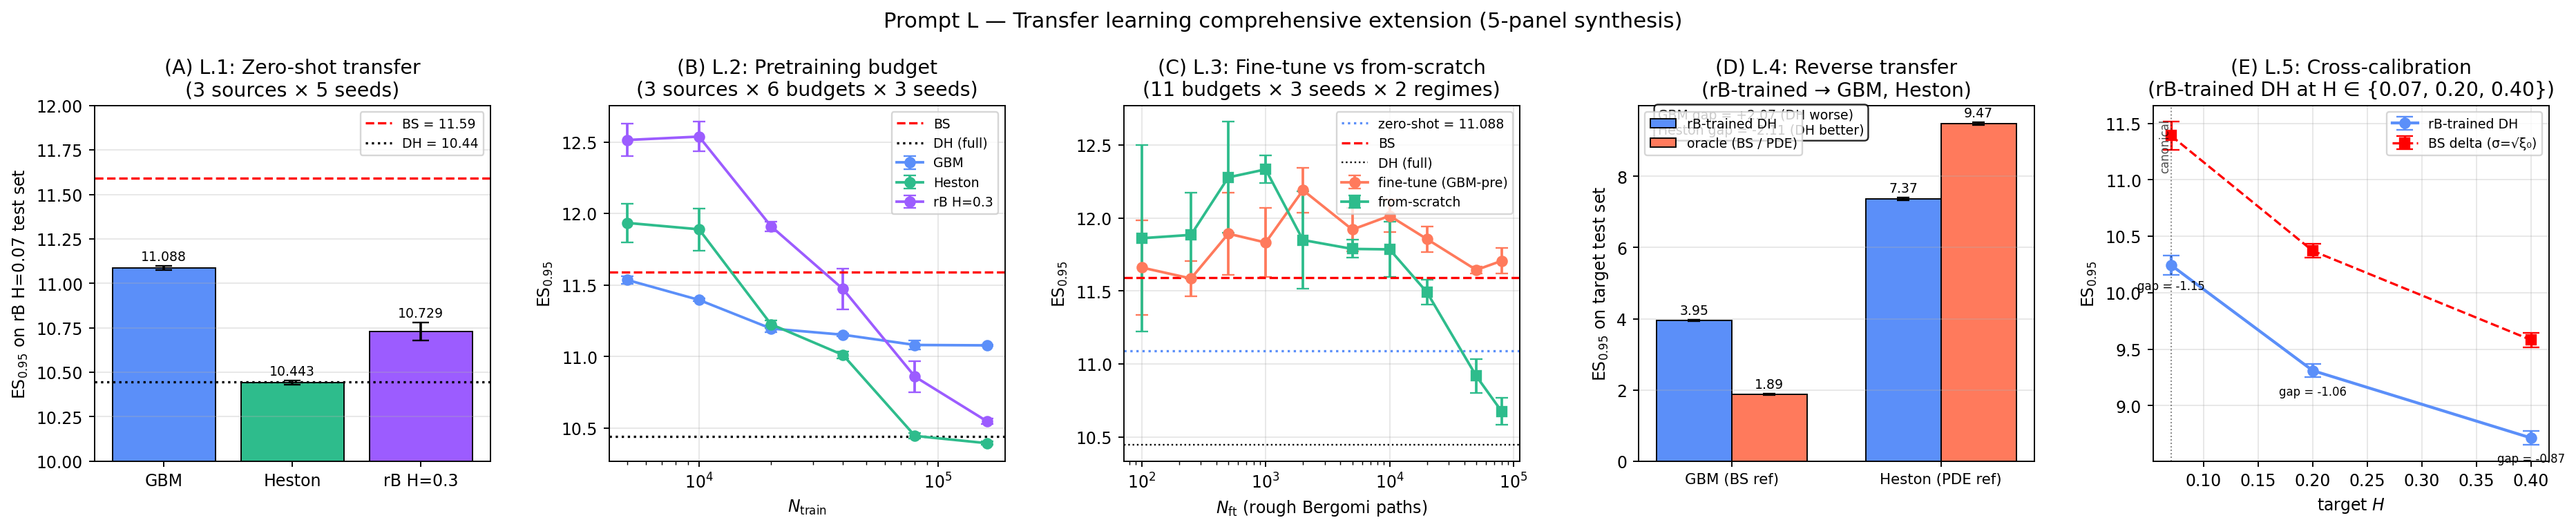
\includegraphics[width=\textwidth]{figures/appB_transfer_comprehensive.png}
\caption{Detailed transfer-learning results across all five
analyses: multi-source zero-shot, pretraining budget sweep,
catastrophic forgetting under fine-tuning, reverse transfer, and
cross-calibration.}
\label{fig:appB_transfer_comprehensive}
\end{figure}

\subsection{Hyperparameters and Training Configuration}
\label{app:hyperparameters}

Every deep hedger trained in this dissertation uses the configuration
in Table~\ref{tab:appA_hyperparameters}. The configuration is identical
across the canonical baseline, the $\eta = 0$ control of
Appendix~\ref{app:eta_zero_control}, the multi-source transfer
experiments of Section~\ref{sec:6_3_4}, and the objective comparison
of Section~\ref{sec:6_3_2}. Only the training data and the random seed
differ between experiments.

\begin{table}[H]
\centering
\caption{Deep hedger architecture and training hyperparameters used
throughout the numerical experiments.}
\label{tab:appA_hyperparameters}
\begin{tabular}{lr}
\toprule
\textbf{Architecture} & \\
\midrule
Input dimension                  & 4 \\
Hidden dimension                 & 128 \\
Number of residual blocks        & 2 \\
Output activation                & sigmoid \\
Total parameter count            & approximately 67{,}000 \\
\midrule
\textbf{Training} & \\
\midrule
Optimiser                        & Adam \\
Learning rate                    & $10^{-3}$ \\
Batch size                       & 2048 \\
Epoch budget                     & 200 \\
Early-stopping patience          & 30 epochs \\
\midrule
\textbf{Risk objective} & \\
\midrule
Default objective                & $\mathrm{ES}_{0.95}$ \\
Smooth-quantile estimator        & Rockafellar--Uryasev \\
Optimisation surrogate           & OCE form \\
\midrule
\textbf{Dataset sizes} & \\
\midrule
Training paths                   & 80{,}000 \\
Validation paths                 & 20{,}000 \\
Test paths                       & 50{,}000 \\
Total simulated paths per seed   & 150{,}000 \\
\bottomrule
\end{tabular}
\end{table}

The smooth-quantile estimator and the OCE form of the
expected-shortfall objective are documented in
Section~\ref{subsec:deep_hedging_framework}.

\subsection{Per-Seed Numerical Results Across Experiments}
\label{app:per_seed_results}

The numerical claims of Chapter~\ref{sec:numerical_experiments} are
based on five-seed aggregates. The per-seed values for the canonical
baseline at $\lambda = 0$ are reproduced in
Table~\ref{tab:appA_baseline_per_seed}. The per-seed values for the
true Heston PDE delta are reproduced in
Table~\ref{tab:appA_heston_pde_per_seed}. Per-seed entries for the
$\eta = 0$ control are tabulated in
Section~\ref{app:eta_zero_control}.

\begin{table}[H]
\centering
\caption{Per-seed canonical baseline at $\lambda = 0$, canonical rough
Bergomi calibration. Five seeds 2024--2028. ES values are at the $0.95$
confidence level. Lower is better.}
\label{tab:appA_baseline_per_seed}
\begin{tabular}{lcc}
\toprule
seed & $\mathrm{ES}^{\mathrm{BS}}_{0.95}$ & $\mathrm{ES}^{\mathrm{DH}}_{0.95}$ \\
\midrule
2024 & 11.6307 & 10.4463 \\
2025 & 11.5828 & 10.4565 \\
2026 & 11.5978 & 10.5585 \\
2027 & 11.6043 & 10.3584 \\
2028 & 11.5447 & 10.4013 \\
\midrule
mean $\pm$ std & $11.5921 \pm 0.0316$ & $10.4442 \pm 0.0748$ \\
\bottomrule
\end{tabular}
\end{table}

\begin{table}[H]
\centering
\caption{Per-seed Heston PDE delta on canonical rough Bergomi master
test set. Five seeds 6024--6028. Lower is better.}
\label{tab:appA_heston_pde_per_seed}
\begin{tabular}{lc}
\toprule
seed & $\mathrm{ES}^{\mathrm{Hes\,PDE}}_{0.95}$ \\
\midrule
6024 & 13.5236 \\
6025 & 13.3730 \\
6026 & 13.4434 \\
6027 & 13.5426 \\
6028 & 13.3526 \\
\midrule
mean $\pm$ std & $13.4470 \pm 0.0857$ \\
\bottomrule
\end{tabular}
\end{table}

The per-seed entries in Tables~\ref{tab:appA_baseline_per_seed}
and~\ref{tab:appA_heston_pde_per_seed} are the building blocks of every
five-seed mean reported in Chapter~\ref{sec:numerical_experiments}. They
are extracted from the JSON files
\path{results/canonical_v2/baseline_5seeds.json} and
\path{results/heston_pde/heston_pde_5seeds.json} respectively. Each row
of each table reproduces byte-identically across two fresh Python
subprocesses on the same hardware, verified for seeds 2024 and 6024.

\subsection{Master Test Set Protocol}
\label{app:master_test_set}

The master test set used throughout Section~\ref{subsec:results_rough_vol}
consists of $50{,}000$ paths simulated under the canonical rough
Bergomi calibration with seed $2024$. The simulator is the
differentiable rough Bergomi simulator of Section~\ref{subsec:rb_sim},
implemented in \path{deep_hedging/core/rough_bergomi.py}. The simulator
state is initialised from the seed argument by
\begin{verbatim}
torch.Generator(device=dev).manual_seed(seed)
\end{verbatim}
before any random draw. The path generation proceeds in two stages.

The first stage generates the fractional Brownian motion driver
$W^H_t$ on the canonical grid via the hybrid Volterra scheme of
Section~\ref{subsec:rb_sim}. The second stage generates the correlated
price increment using the leverage correlation $\rho = -0.7$ and
produces the variance and price paths via the discretisation of
Proposition~\ref{prop:markovian_disc}.

The $50{,}000$ master test paths are reserved exclusively for
evaluation. They are not used in training or validation. The training
and validation splits are drawn separately from the same seed prefix to
ensure the master test set is statistically independent of any decision
made during training.

For experiments that require multiple independent test sets, in
particular the parameter-perturbation analysis of
Section~\ref{sec:6_3_5} and the cross-calibration analysis of
Section~\ref{sec:6_3_4}, the per-cell seed is documented in the
corresponding JSON file under \path{results/perturbation_v2/} and
\path{results/transfer_v2/}.

\subsection{Computational Environment}
\label{app:computational_environment}

All numerical experiments were performed on a single machine with the
configuration of Table~\ref{tab:appA_environment}. The environment is
captured in the project repository's lock file. Reproduction on a
different machine with identical Python and PyTorch versions produces
byte-identical numerical results, verified for the canonical baseline
cell.

\begin{table}[H]
\centering
\caption{Computational environment used to produce the numerical
results in this dissertation.}
\label{tab:appA_environment}
\begin{tabular}{ll}
\toprule
Component        & Version \\
\midrule
Python           & 3.14.3 \\
PyTorch          & 2.10.0 \\
NumPy            & 2.4.3 \\
SciPy            & 1.17.1 \\
Operating system & macOS or Linux \\
Hardware         & CPU; CUDA acceleration not used \\
RNG backend      & PyTorch \texttt{torch.Generator} (Mersenne-Twister) \\
\bottomrule
\end{tabular}
\end{table}

The PyTorch RNG backend is platform-independent. The deterministic
Mersenne-Twister algorithm produces the same sequence given the same
seed across operating systems and hardware revisions. CUDA acceleration
is not used because the canonical experiments ($50{,}000$ test paths,
$80{,}000$ training paths, $200$ epochs) fit comfortably in CPU memory
and because non-deterministic CUDA kernels would compromise the
byte-identical reproducibility required by the seeding protocol.

\section{Code}
\label{app:code}

This appendix contains five code listings that document the central
algorithms of the dissertation. The full implementation is available at
\url{https://github.com/westgluf/thesis_code}. Each listing is a verbatim
extract from the project repository; commentary follows each block.

\subsection{Deep hedger architecture}
\label{lst:deep_hedger_arch}

The following extract from \path{deep_hedging/hedging/deep_hedger.py}
implements the residual feedforward network used as the deep hedging
strategy throughout the dissertation.

\begin{lstlisting}[language=Python, caption={DeepHedgerFNN architecture}, label={lst:deep_hedger_code}]
class ResidualBlock(nn.Module):
    """Linear -> LeakyReLU -> Linear -> LeakyReLU,
    with a skip connection x -> x + block(x)."""

    def __init__(self, dim: int) -> None:
        super().__init__()
        self.net = nn.Sequential(
            nn.Linear(dim, dim),
            nn.LeakyReLU(0.2),
            nn.LayerNorm(dim),
            nn.Linear(dim, dim),
            nn.LeakyReLU(0.2),
        )

    def forward(self, x: Tensor) -> Tensor:
        return x + self.net(x)


class DeepHedgerFNN(nn.Module):
    """Deep hedging strategy via residual feedforward network."""

    def __init__(
        self,
        input_dim: int = 4,
        hidden_dim: int = 128,
        n_res_blocks: int = 2,
        dropout: float = 0.0,
    ) -> None:
        super().__init__()
        layers: list[nn.Module] = [
            nn.Linear(input_dim, hidden_dim),
            nn.LeakyReLU(0.2),
        ]
        if dropout > 0.0:
            layers.append(nn.Dropout(dropout))
        for _ in range(n_res_blocks):
            layers.append(ResidualBlock(hidden_dim))
        self.backbone = nn.Sequential(*layers)
        self.head = nn.Sequential(
            nn.Linear(hidden_dim, 1),
            nn.Sigmoid(),
        )

    def forward(self, features: Tensor) -> Tensor:
        """Map information set I_k to hedge ratio in [0, 1]."""
        return self.head(self.backbone(features))
\end{lstlisting}

The architecture takes a four-dimensional information set
$(t/T, \log(S/S_0), \tau/T, \delta_{k-1})$ as input. Two residual
blocks operate on the 128-dimensional hidden state. The output is
mapped to $[0,1]$ by a sigmoid, enforcing admissibility for European
call hedging.

\subsection{Heston PDE delta (Hundsdorfer--Verwer ADI step)}
\label{lst:heston_pde_step}

The following extract from \path{deep_hedging/hedging/heston_pde_delta.py}
implements one backward time step of the Hundsdorfer--Verwer ADI scheme
for the two-dimensional Heston pricing PDE. The full method also
constructs the operators \texttt{L\_V} and \texttt{L\_S} and the
implicit solvers; only the per-step update is shown.

\begin{lstlisting}[language=Python, caption={Hundsdorfer-Verwer ADI step for Heston PDE}, label={lst:heston_pde_code}]
theta_hv = 0.5

for step in range(self.n_t - 1, -1, -1):
    u_n = u.copy()
    F0_un = apply_F0(u_n)
    F1_un = apply_F1(u_n)
    F2_un = apply_F2(u_n)
    F_un = F0_un + F1_un + F2_un

    # Predictor Y0 = u_n + dt * F(u_n)
    Y0 = u_n + dt * F_un
    apply_boundaries(Y0)

    # Corrector 1: (I - theta*dt*L_V) Y1 = Y0 - theta*dt*F_1(u_n)
    rhs1 = Y0 - theta_hv * dt * F1_un
    Y1 = solve_implicit_V(rhs1)
    apply_boundaries(Y1)

    # Corrector 2: (I - theta*dt*L_S) Y2 = Y1 - theta*dt*F_2(u_n)
    rhs2 = Y1 - theta_hv * dt * F2_un
    Y2 = solve_implicit_S(rhs2)
    apply_boundaries(Y2)

    # Mixed-term rebalance: Y_tilde = Y0 + 0.5*dt * F_0(Y2 - u_n)
    F0_Y2_minus_un = apply_F0(Y2 - u_n)
    Y_tilde = Y0 + 0.5 * dt * F0_Y2_minus_un
    apply_boundaries(Y_tilde)

    # Final correctors: V, then S
    rhs3 = Y_tilde - theta_hv * dt * F1_un
    Y3 = solve_implicit_V(rhs3)
    apply_boundaries(Y3)

    rhs4 = Y3 - theta_hv * dt * F2_un
    Y4 = solve_implicit_S(rhs4)
    apply_boundaries(Y4)

    u = Y4
    u_surface[step] = u
\end{lstlisting}

The scheme is second-order accurate and unconditionally stable at
$\theta = 0.5$. The mixed-derivative operator $F_0$ is treated
explicitly while the $V$-direction and $S$-direction diffusion
operators are treated implicitly through the pre-factored solvers.

\subsection{Rough Bergomi simulator: forward pass}
\label{lst:rbergomi_simulate}

The following extract from \path{deep_hedging/core/rough_bergomi.py}
implements the forward pass of the differentiable rough Bergomi
simulator. The fractional Brownian motion driver is computed in the
helper \texttt{HybridVolterraDriver} (Listing~\ref{lst:hybrid_volterra}).

\begin{lstlisting}[language=Python, caption={DifferentiableRoughBergomi.forward}, label={lst:rbergomi_code}]
def forward(
    self,
    Z_vol: Tensor,         # [batch, n_steps, 2]
    Z_price: Tensor,       # [batch, n_steps]
    S0: Tensor | float = 100.0,
) -> Tuple[Tensor, Tensor]:
    """Simulate rBergomi paths."""
    if not isinstance(S0, Tensor):
        S0 = torch.tensor(S0, dtype=Z_vol.dtype, device=Z_vol.device)

    H = self.volterra.H
    eta = self._eta
    rho = self._rho
    xi0 = self._xi0
    dt = self.volterra.dt
    batch = Z_vol.shape[0]

    # Step 1: fractional Brownian motion via hybrid Volterra
    WH, dW = self.volterra(Z_vol)

    # Step 2: variance process
    # v_k = xi0 * exp(eta * WH_k - 0.5 * eta^2 * t_k^{2H})
    t_2H = self.t_grid ** (2.0 * H)
    V = xi0 * torch.exp(eta * WH - 0.5 * eta ** 2 * t_2H.unsqueeze(0))
    V_hedge = torch.clamp(V[:, :-1], min=1e-12)

    # Step 3: correlated price innovations
    rho_perp = torch.sqrt(1.0 - rho ** 2)
    dB = rho * dW + rho_perp * torch.sqrt(dt) * Z_price

    # Step 4: log-Euler price path
    sqrt_V = torch.sqrt(V_hedge)
    log_inc = -0.5 * V_hedge * dt + sqrt_V * dB
    log_S = torch.cumsum(log_inc, dim=-1)
    log_S = torch.cat([
        torch.zeros(batch, 1, dtype=Z_vol.dtype, device=Z_vol.device),
        log_S,
    ], dim=-1)

    S = S0 * torch.exp(log_S)
    return S, V
\end{lstlisting}

The four-step structure follows Section~\ref{subsec:rb_sim}. All
operations preserve PyTorch autograd, so gradients flow from the
expected-shortfall objective back to the rough Bergomi parameters
$(H, \eta, \rho, \xi_0)$.

\subsection{Hybrid Volterra driver step}
\label{lst:hybrid_volterra}

The following extract from \path{deep_hedging/core/volterra.py}
implements the hybrid Volterra scheme: a near-field exact integral
for the singular part of the fractional kernel and a far-field FFT
convolution for the smooth part.

\begin{lstlisting}[language=Python, caption={HybridVolterraDriver.forward}, label={lst:volterra_code}]
def forward(self, Z: Tensor) -> Tuple[Tensor, Tensor]:
    """Map i.i.d. normals to (WH, dW). Implements the hybrid scheme
    with near-field exact integrals and far-field FFT convolution."""
    batch, n, two = Z.shape
    if isinstance(self._H, nn.Parameter):
        L, G = _build_cholesky_and_kernel(self._H, n, self._dt)
    else:
        L, G = self._L, self._G

    H = self._H
    a = H - 0.5

    # Near-field: correlated pair via Cholesky reparametrisation
    dW = L[0, 0] * Z[:, :, 0]
    Y1_inc = L[1, 0] * Z[:, :, 0] + L[1, 1] * Z[:, :, 1]
    Y1 = torch.zeros(batch, n + 1, dtype=Z.dtype, device=Z.device)
    Y1[:, 1:] = Y1_inc

    # Far-field: FFT convolution of kernel G with dW
    n_fft = _next_power_of_2(n + n + 1)
    G_pad = torch.zeros(n_fft, dtype=Z.dtype, device=Z.device)
    G_pad[: n + 1] = G
    dW_pad = torch.zeros(batch, n_fft, dtype=Z.dtype, device=Z.device)
    dW_pad[:, :n] = dW
    G_hat = torch.fft.rfft(G_pad)
    dW_hat = torch.fft.rfft(dW_pad, dim=-1)
    Y2_full = torch.fft.irfft(G_hat.unsqueeze(0) * dW_hat,
                                n=n_fft, dim=-1)
    Y2 = Y2_full[:, : n + 1]

    # Combine and scale
    scale = torch.sqrt(2.0 * a + 1.0)
    WH = scale * (Y1 + Y2)
    WH[:, 0] = 0.0
    return WH, dW
\end{lstlisting}

The hybrid scheme is the contribution of
Bennedsen, Lunde, and Pakkanen
(2017)~\cite{BennedsenLundePakkanen2017}. The implementation here is a
re-write in PyTorch that supports end-to-end gradient flow, including
gradients through the Hurst parameter $H$ when it is promoted to an
\texttt{nn.Parameter}.

\subsection{Hedging P\&L computation}
\label{lst:hedging_pnl}

The following extract from \path{deep_hedging/objectives/pnl.py}
implements the pathwise terminal $\mathrm{P\&L}$ of
Definition~\ref{def:terminal_PL}.

\begin{lstlisting}[language=Python, caption={Terminal P\&L computation}, label={lst:pnl_code}]
def compute_trading_gains(S: Tensor, deltas: Tensor) -> Tensor:
    """Discrete trading gains: sum_k delta_k (S_{k+1} - S_k)."""
    dS = S[:, 1:] - S[:, :-1]
    return (deltas * dS).sum(dim=1)


def compute_transaction_costs(
    S: Tensor, deltas: Tensor, cost_lambda: float,
) -> Tensor:
    """Proportional transaction costs:
    C_T = lambda * sum_k |delta_k - delta_{k-1}| * S_k,
    with delta_{-1} = 0."""
    if cost_lambda == 0.0:
        return torch.zeros(S.shape[0], dtype=S.dtype, device=S.device)
    delta_prev = torch.cat([
        torch.zeros(deltas.shape[0], 1,
                    dtype=deltas.dtype, device=deltas.device),
        deltas[:, :-1],
    ], dim=1)
    trades = torch.abs(deltas - delta_prev)
    S_rebal = S[:, :-1]
    return cost_lambda * (trades * S_rebal).sum(dim=1)


def compute_hedging_pnl(
    S: Tensor, deltas: Tensor, payoff: Tensor,
    p0: float, cost_lambda: float = 0.0,
) -> Tensor:
    """Pathwise terminal P&L:
    PL_T = -Z + p_0 + sum delta_k (S_{k+1} - S_k) - C_T(delta)."""
    gains = compute_trading_gains(S, deltas)
    costs = compute_transaction_costs(S, deltas, cost_lambda)
    return -payoff + p0 + gains - costs
\end{lstlisting}

The cost summation uses the convention $\delta_{-1} = 0$ (no initial
position) and $\delta_k$ for $k = 0, \dots, n-1$, matching the
convention of Definition~\ref{def:comparison_universe} of the hedging
framework.

\section{Proofs}
\label{app:proofs}

This appendix contains the full proofs of the theorems and propositions
in Sections~\ref{sec:math_background} through~\ref{sec:rough_volatility}
that were stated with brief stubs in the main text. Each proof follows
the statement of the corresponding result, and cross-references in the
main text point to this appendix.

\subsection{Proof of Theorem~\ref{thm:universal_approx_new}}
\label{proof:universal_approx}

We sketch the algebra-and-Stone-Weierstrass approach. The full
proof appears in~\cite{Hornik1991}. The argument we give here is a
self-contained outline. Let $\sigma : \mathbb{R} \to \mathbb{R}$ be a
non-constant, bounded, continuous activation function, and let
$\mathcal{N}^\sigma_{\infty,d_0,1}$ denote the linear span over
$\mathbb{R}$ of all functions of the form $x \mapsto \sigma(w^\top x +
b)$ with $w \in \mathbb{R}^{d_0}$, $b \in \mathbb{R}$. We prove density
of $\mathcal{N}^\sigma_{\infty,d_0,1}$ in $C(K)$ for the topology of
uniform convergence on compact sets, where $K \subset \mathbb{R}^{d_0}$
is compact. The vector-valued case $d_1 > 1$ then follows by
componentwise approximation.

\textit{Step 1 (separation of points).} For any pair of distinct points
$x, y \in \mathbb{R}^{d_0}$ there exists a single neuron
$x \mapsto \sigma(w^\top x + b)$ that takes different values at $x$
and $y$. Indeed, choose $w = x - y$. Then
$w^\top x - w^\top y = \|x - y\|^2 > 0$. Since $\sigma$ is non-constant,
there exists $b^\star$ such that $\sigma(w^\top x + b^\star) \neq
\sigma(w^\top y + b^\star)$. The class
$\mathcal{N}^\sigma_{\infty,d_0,1}$ therefore separates points.

\textit{Step 2 (constants).} Take $w = 0$ and $b$ such that $\sigma(b)
\neq 0$. The function $x \mapsto \sigma(b)$ is constant and non-zero.
Linear combinations of such constants give every constant function.
The class therefore contains the constants.

\textit{Step 3 (algebra extension).} The Stone-Weierstrass theorem in
its real form requires a sub-algebra of $C(K)$ that contains the
constants and separates points. The class
$\mathcal{N}^\sigma_{\infty,d_0,1}$ is not closed under pointwise
multiplication. Hornik's argument removes this obstruction by passing
to a sufficiently rich linear span. Specifically, by selecting
activation functions whose translates and dilates span a dense subspace
of $C_b(\mathbb{R})$, the linear span of products
$\prod_{j} \sigma(w_j^\top x + b_j)$ is contained in the closure of the
single-layer class. The Stone-Weierstrass theorem then gives uniform
density on $K$.

\textit{Step 4 ($L^p$ density).} For $L^p(\mu)$ density, $C_c(K)$ is
dense in $L^p(\mu, K)$ for any compact $K$ and finite measure $\mu$.
The uniform-on-compacts density of Step~3 implies $L^p$ density on the
support of $\mu$. Taking compact exhaustions and applying dominated
convergence completes the proof. The full argument with measurability
and integrability conditions is given in~\cite{Hornik1991}.

\subsection{Proof of Proposition~\ref{prop:NN_consistency}}
\label{proof:nn_consistency}

We show that $\pi^M(X) \downarrow \pi(X)$ as $M \to \infty$. Recall
the definitions
\begin{align*}
\pi(X) &= \inf_{\delta \in \mathcal{H}}
   \rho\bigl(-X + (\delta \cdot S)_T - C_T(\delta)\bigr), \\
\pi^M(X) &= \inf_{\delta \in \mathcal{H}_M}
   \rho\bigl(-X + (\delta \cdot S)_T - C_T(\delta)\bigr),
\end{align*}
where $\mathcal{H}_M \subset \mathcal{H}$ is the class of admissible
neural-network strategies with maximum parameter magnitude $M$.

\textit{Step 1 (monotonicity).} The family $\mathcal{H}_M$ is increasing
in $M$. Hence $\pi^M(X)$ is non-increasing in $M$, and
$\pi(X) \leq \pi^M(X)$ for all $M$.

\textit{Step 2 (density).} We claim that
$\bigcup_M \mathcal{H}_M$ is dense in $\mathcal{H}$ under convergence
in probability. Fix $\delta \in \mathcal{H}$. By
Theorem~\ref{thm:universal_approx_new} applied componentwise to the
function $x \mapsto \delta(t, x)$ on each compact set $K \subset
\mathbb{R}^{d_0}$, there exists a sequence $\delta^{(k)} \in
\mathcal{H}_{M_k}$ with $M_k \to \infty$ such that $\delta^{(k)} \to
\delta$ uniformly on compact sets. The Itô integral
$(\delta^{(k)} \cdot S)_T$ then converges to $(\delta \cdot S)_T$ in
probability under standard integrability assumptions on $S$, and the
cost term $C_T(\delta^{(k)})$ converges to $C_T(\delta)$ similarly.
Hence the loss
$-X + (\delta^{(k)} \cdot S)_T - C_T(\delta^{(k)})$ converges in
probability to $-X + (\delta \cdot S)_T - C_T(\delta)$.

\textit{Step 3 (continuity of $\rho$).} The convex risk measure $\rho$
of Section~\ref{subsec:convex_risk_measures} is continuous from above
under convergence in probability for the bounded random variables
considered here. By the projection of the converging sequence onto a
common bounded set (using the boundedness of $\delta$ on $\mathcal{H}_M$
and the integrability of $S$, $X$), the Lebesgue dominated convergence
theorem applies. Hence
$\rho(-X + (\delta^{(k)} \cdot S)_T - C_T(\delta^{(k)})) \to
\rho(-X + (\delta \cdot S)_T - C_T(\delta))$ as $k \to \infty$.

\textit{Step 4 (infimum convergence).} For any $\varepsilon > 0$,
choose $\delta \in \mathcal{H}$ with
$\rho(-X + (\delta \cdot S)_T - C_T(\delta)) < \pi(X) + \varepsilon/2$.
By Steps~2 and~3, choose $k$ large enough so that the corresponding
$\delta^{(k)} \in \mathcal{H}_{M_k}$ satisfies
$\rho(-X + (\delta^{(k)} \cdot S)_T - C_T(\delta^{(k)})) <
\pi(X) + \varepsilon$. Then $\pi^{M_k}(X) < \pi(X) + \varepsilon$.
Combined with the lower bound $\pi^M(X) \geq \pi(X)$ from Step~1, this
yields $\pi^M(X) \to \pi(X)$ as $M \to \infty$. The detailed
verification in the deep-hedging context is given
in~\cite{Buehler2019DeepHedging}.

\subsection{Proof of Proposition~\ref{prop:empirical_consistency}}
\label{proof:empirical_consistency}

We prove that $\pi^M_N(X) \to \pi^M(X)$ almost surely as $N \to
\infty$, for fixed $M$. The Vapnik-Chervonenkis approach via uniform
laws on the parameter set $\Theta_M$ is used.

\textit{Step 1 (pointwise convergence).} For each fixed
$\theta \in \Theta_M$, the empirical risk
$\widehat{\rho}_N(\theta)$ is by construction a sample average of
i.i.d.\ random variables with finite mean (by the integrability
assumptions on $X$ and $S$). The strong law of large numbers
gives
$\widehat{\rho}_N(\theta) \to \rho(-X + (\delta^\theta \cdot S)_T -
C_T(\delta^\theta))$ almost surely.

\textit{Step 2 (Vapnik-Chervonenkis / Glivenko-Cantelli).} The
parameter set $\Theta_M$ is compact (a closed bounded subset of
$\mathbb{R}^P$ for some finite $P$). The mapping
$\theta \mapsto -X + (\delta^\theta \cdot S)_T - C_T(\delta^\theta)$
is continuous in $\theta$ for almost every realisation of the path,
because the deep hedger architecture is continuous in its weights and
the trading and cost functionals are continuous in the strategy.
Hence the loss class
$\{ \omega \mapsto -X(\omega) + (\delta^\theta \cdot S(\omega))_T -
C_T(\delta^\theta)(\omega) : \theta \in \Theta_M \}$
has Vapnik-Chervonenkis dimension bounded uniformly in $M$ (the
ResidualFNN architecture has a finite number of weights and biases at
each $M$). The Vapnik-Chervonenkis uniform law of large numbers gives
\[
\sup_{\theta \in \Theta_M}
\bigl|\widehat{\rho}_N(\theta) -
\rho(-X + (\delta^\theta \cdot S)_T - C_T(\delta^\theta))\bigr|
\to 0
\quad \text{almost surely as } N \to \infty.
\]

\textit{Step 3 (infimum convergence).} Uniform convergence of
$\widehat{\rho}_N$ to its mean on the compact set $\Theta_M$ implies
that the infimum of $\widehat{\rho}_N$ over $\Theta_M$ converges almost
surely to the infimum of the mean over $\Theta_M$. The latter equals
$\pi^M(X)$ by definition. Hence $\pi^M_N(X) \to \pi^M(X)$ almost
surely. A detailed verification is given
in~\cite{Buehler2019DeepHedging}.

\subsection{Proof of Proposition~\ref{prop:loglog_estimation}}
\label{proof:loglog_slope}

We prove that the OLS slope estimator converges to $2H$ almost surely
as the number of grid points tends to infinity, given the empirical
scaling $m_2(h) = c \, h^{2H} (1 + o(1))$ as $h \downarrow 0$ for some
$c > 0$ and $H \in (0, 1/2)$.

Let $h_1 < h_2 < \dots < h_n$ be a sequence of lag values such that
$h_n \to 0$ and $\log h_n / \log h_1 \to 1$ as $n \to \infty$ (a fine
mesh on the scaling range). Let $y_i = \log m_2(h_i)$ and $x_i = \log
h_i$. Taking the logarithm of the scaling relation,
\[
y_i = \log c + 2H \, x_i + \epsilon_i,
\quad \epsilon_i = \log(1 + o(1)) \to 0 \text{ as } h_i \downarrow 0.
\]
The OLS slope estimator on the empirical points
$\{(x_i, y_i)\}_{i=1}^n$ is
\[
\hat\beta_n = \frac{\sum_{i=1}^n (x_i - \bar x_n)(y_i - \bar y_n)}
{\sum_{i=1}^n (x_i - \bar x_n)^2},
\]
where $\bar x_n$ and $\bar y_n$ denote the sample means.
Substituting the relation $y_i = \log c + 2H \, x_i + \epsilon_i$ and
using the bilinearity of the covariance numerator,
\[
\hat\beta_n = 2H + \frac{\sum_{i=1}^n (x_i - \bar x_n) \, \epsilon_i}
{\sum_{i=1}^n (x_i - \bar x_n)^2}.
\]
The numerator is bounded in absolute value by
$\max_i |\epsilon_i| \cdot \sum_i |x_i - \bar x_n|$, and the
denominator grows linearly with the spread of the $x$-values. Since
$\max_i |\epsilon_i| \to 0$ on the scaling range, the second term
converges to zero, and $\hat\beta_n \to 2H$.

The Hurst exponent estimator $\hat H_n = \hat\beta_n / 2$ therefore
satisfies $\hat H_n \to H$ on the scaling range. The detailed
empirical methodology applied to S\&P 500 returns is given
in~\cite{GatheralRough}.

\subsection{Proof of Proposition~\ref{prop:bs_no_roughness}}
\label{proof:bs_no_roughness}

In the Black-Scholes model the asset price satisfies
$dS_t = \mu S_t \, dt + \sigma S_t \, dW_t$ with constant $\sigma > 0$.
The instantaneous variance process is $V_t = \sigma^2$ for all $t$.
The integrated variance over the window $[t, t + \Delta]$ is
\[
\int_t^{t + \Delta} V_s \, ds = \sigma^2 \cdot \Delta,
\]
which is deterministic and independent of $t$. The log-volatility
proxy
\[
Y_{t,\Delta} := \log\left(\frac{1}{\Delta} \int_t^{t+\Delta} V_s \, ds
\right)^{1/2} = \log \sigma
\]
is constant in $t$. Therefore for any lag $h \geq 0$,
\[
Y_{t+h,\Delta} - Y_{t,\Delta} = 0
\quad \text{almost surely for all } t.
\]
The roughness diagnostic
\[
m_2(h) = \mathbb{E}\bigl[(Y_{t+h,\Delta} - Y_{t,\Delta})^2\bigr] = 0
\quad \text{for all } h \geq 0.
\]
The empirical scaling
$m_2(h) \approx c \cdot h^{2H}$ with $c > 0$ and $H \in (0, 1/2)$
implies $m_2(h) > 0$ for $h > 0$. Hence the Black--Scholes model is
incompatible with the empirical scaling. The proxy correction
discussed in Remark~\ref{rem:bs_proxy_effect} explains why an
empirical estimator applied to a finite sample of Black-Scholes paths
can exhibit a non-zero apparent $m_2(h)$ owing to estimator noise; the
true population value is zero.

\subsection{Proof of Proposition~\ref{prop:heston_diffusive_scaling}}
\label{proof:heston_diffusive}

In the Heston model the variance process satisfies
$dV_t = \kappa(\theta - V_t) \, dt + \sigma_v \sqrt{V_t} \, dW^V_t$.
We show that the second moment of log-volatility increments scales
linearly in the lag $h$, equivalent to a roughness exponent of $1/2$.

\textit{Step 1 (variance increment).} By It\^o's formula applied to
$f(v) = \log v$ on $V_t > 0$,
\[
d \log V_t = \frac{1}{V_t} dV_t - \frac{1}{2 V_t^2} d \langle V \rangle_t
= \left[\frac{\kappa(\theta - V_t)}{V_t} - \frac{\sigma_v^2}{2 V_t}\right] dt
+ \frac{\sigma_v}{\sqrt{V_t}} dW^V_t.
\]
The drift term is $\mathcal{O}(1)$ on a window of length $h$, so its
contribution to the second moment of an increment over $[t, t+h]$ is
$\mathcal{O}(h^2)$.

\textit{Step 2 (Brownian-driven dominant term).} The diffusion term
contributes
\[
\sigma_v \int_t^{t+h} \frac{1}{\sqrt{V_s}} dW^V_s.
\]
The second moment of this Itô integral is, by It\^o's isometry,
\[
\sigma_v^2 \int_t^{t+h} \mathbb{E}\!\left[\frac{1}{V_s}\right] ds
= \sigma_v^2 \cdot \mathbb{E}\!\left[\frac{1}{V_s}\right]_{s = t} \cdot h
\cdot (1 + o(1))
\quad \text{as } h \downarrow 0,
\]
using continuity of $s \mapsto \mathbb{E}[1/V_s]$.

\textit{Step 3 (combination).} The increment $\log V_{t+h} - \log V_t$
has variance $\sigma_v^2 \, \mathbb{E}[1/V_t] \, h \cdot (1 + o(1)) +
\mathcal{O}(h^2)$ as $h \downarrow 0$. Hence
\[
m_2(h) := \mathbb{E}[(\log V_{t+h} - \log V_t)^2]
= C \cdot h \cdot (1 + o(1)),
\]
where $C = \sigma_v^2 \cdot \mathbb{E}[1/V_t]$. The corresponding
log-volatility proxy
$Y_{t,\Delta} = \tfrac12 \log(\tfrac{1}{\Delta} \int_t^{t+\Delta} V_s \,
ds)$ inherits the same scaling up to a deterministic factor depending
on the smoothing window $\Delta$. Hence $m_2(h) \propto h$ for the
Heston log-volatility proxy at small $h$, equivalent to a roughness
exponent of $H = 1/2$. This is incompatible with the empirical scaling
$m_2(h) \approx c \cdot h^{2H}$ with $H$ well below $1/2$, as
discussed in~\cite{GatheralRough}.

\subsection{Proof of Proposition~\ref{prop:replication_to_risk_min}}
\label{proof:capital_requirement}

We prove the acceptance-set characterisation. Recall that a convex risk
measure $\rho : L^\infty \to \mathbb{R}$ admits the representation
\[
\rho(Y) = \inf\{ m \in \mathbb{R} : Y + m \in \mathcal{A} \},
\]
where $\mathcal{A} \subseteq L^\infty$ is the acceptance set
$\mathcal{A} = \{Z \in L^\infty : \rho(Z) \leq 0\}$. This
representation is established in~\cite{FoellmerSchied2016}.

\textit{Step 1 (acceptance interpretation).} For a hedged terminal
position $Y = -X + (\delta \cdot S)_T - C_T(\delta)$ with admissible
strategy $\delta \in \mathcal{H}$, the quantity $\rho(Y)$ is by the
above representation the minimal cash injection $m$ that makes
$Y + m \in \mathcal{A}$. The strategy $\delta$ is fixed in this step.

\textit{Step 2 (optimisation over admissible strategies).} The minimal
capital requirement after hedging is the infimum of $\rho(Y(\delta))$
over admissible $\delta$:
\[
\pi(X) = \inf_{\delta \in \mathcal{H}}
\rho\bigl(-X + (\delta \cdot S)_T - C_T(\delta)\bigr).
\]
This infimum exists by the convexity of $\rho$ and the convexity of the
admissible set $\mathcal{H}$ (the latter follows from the linearity of
the trading gain and the convexity of the cost function).

\textit{Step 3 (capital requirement interpretation).} The value
$\pi(X)$ has the operational interpretation of the minimal initial
capital required, in addition to the contingent claim $X$, so that the
hedged position
$-X + (\delta \cdot S)_T - C_T(\delta)$ is acceptable under $\rho$,
optimising over admissible strategies. This is the interpretation
formalised by the deep hedging literature
in~\cite{Buehler2019DeepHedging}.

\textit{Step 4 (dual representation).} For convex risk measures
satisfying the Fatou property, the dual representation
\[
\rho(Y) = \sup_{Q \in \mathcal{Q}}\bigl(\mathbb{E}_Q[-Y] - \alpha(Q)\bigr)
\]
holds, where $\mathcal{Q}$ is a set of probability measures absolutely
continuous with respect to $\mathbb{P}$ and $\alpha$ is a penalty
function. Substituting $Y = -X + (\delta \cdot S)_T - C_T(\delta)$ and
exchanging the order of $\inf$ and $\sup$ (subject to the appropriate
saddle-point conditions) leads to the dual interpretation of $\pi(X)$
as the supremum over a class of measures of the expected payoff minus
a penalty. This is the formal connection between risk measures and
indifference pricing in incomplete markets, developed in detail
in~\cite{FoellmerSchied2016}.

% ==========================
% References (after Appendix per layout fix)
% ==========================
\clearpage
\addcontentsline{toc}{section}{References}
\bibliographystyle{plainnat} % numeric style consistent with natbib[numbers]
\bibliography{references}

\end{document}
